\batchmode
\documentclass[twoside]{book}

% Packages required by doxygen
\usepackage{calc}
\usepackage{doxygen}
\usepackage{graphicx}
\usepackage[utf8]{inputenc}
\usepackage{makeidx}
\usepackage{multicol}
\usepackage{multirow}
\usepackage{fixltx2e}
\PassOptionsToPackage{warn}{textcomp}
\usepackage{textcomp}
\usepackage[nointegrals]{wasysym}
\usepackage[table]{xcolor}

% Font selection
\usepackage[T1]{fontenc}
\usepackage{mathptmx}
\usepackage[scaled=.90]{helvet}
\usepackage{courier}
\usepackage{amssymb}
\usepackage{sectsty}
\renewcommand{\familydefault}{\sfdefault}
\allsectionsfont{%
  \fontseries{bc}\selectfont%
  \color{darkgray}%
}
\renewcommand{\DoxyLabelFont}{%
  \fontseries{bc}\selectfont%
  \color{darkgray}%
}
\newcommand{\+}{\discretionary{\mbox{\scriptsize$\hookleftarrow$}}{}{}}

% Page & text layout
\usepackage{geometry}
\geometry{%
  letterpaper,%
  top=2.5cm,%
  bottom=2.5cm,%
  left=2.5cm,%
  right=2.5cm%
}
\tolerance=750
\hfuzz=15pt
\hbadness=750
\setlength{\emergencystretch}{15pt}
\setlength{\parindent}{0cm}
\setlength{\parskip}{0.2cm}
\makeatletter
\renewcommand{\paragraph}{%
  \@startsection{paragraph}{4}{0ex}{-1.0ex}{1.0ex}{%
    \normalfont\normalsize\bfseries\SS@parafont%
  }%
}
\renewcommand{\subparagraph}{%
  \@startsection{subparagraph}{5}{0ex}{-1.0ex}{1.0ex}{%
    \normalfont\normalsize\bfseries\SS@subparafont%
  }%
}
\makeatother

% Headers & footers
\usepackage{fancyhdr}
\pagestyle{fancyplain}
\fancyhead[LE]{\fancyplain{}{\bfseries\thepage}}
\fancyhead[CE]{\fancyplain{}{}}
\fancyhead[RE]{\fancyplain{}{\bfseries\leftmark}}
\fancyhead[LO]{\fancyplain{}{\bfseries\rightmark}}
\fancyhead[CO]{\fancyplain{}{}}
\fancyhead[RO]{\fancyplain{}{\bfseries\thepage}}
\fancyfoot[LE]{\fancyplain{}{}}
\fancyfoot[CE]{\fancyplain{}{}}
\fancyfoot[RE]{\fancyplain{}{\bfseries\scriptsize Generated on Tue Jul 28 2015 22\+:27\+:22 for Vespucci by Doxygen }}
\fancyfoot[LO]{\fancyplain{}{\bfseries\scriptsize Generated on Tue Jul 28 2015 22\+:27\+:22 for Vespucci by Doxygen }}
\fancyfoot[CO]{\fancyplain{}{}}
\fancyfoot[RO]{\fancyplain{}{}}
\renewcommand{\footrulewidth}{0.4pt}
\renewcommand{\chaptermark}[1]{%
  \markboth{#1}{}%
}
\renewcommand{\sectionmark}[1]{%
  \markright{\thesection\ #1}%
}

% Indices & bibliography
\usepackage{natbib}
\usepackage[titles]{tocloft}
\setcounter{tocdepth}{3}
\setcounter{secnumdepth}{5}
\makeindex

% Hyperlinks (required, but should be loaded last)
\usepackage{ifpdf}
\ifpdf
  \usepackage[pdftex,pagebackref=true]{hyperref}
\else
  \usepackage[ps2pdf,pagebackref=true]{hyperref}
\fi
\hypersetup{%
  colorlinks=true,%
  linkcolor=blue,%
  citecolor=blue,%
  unicode%
}

% Custom commands
\newcommand{\clearemptydoublepage}{%
  \newpage{\pagestyle{empty}\cleardoublepage}%
}


%===== C O N T E N T S =====

\begin{document}

% Titlepage & ToC
\hypersetup{pageanchor=false,
             bookmarks=true,
             bookmarksnumbered=true,
             pdfencoding=unicode
            }
\pagenumbering{roman}
\begin{titlepage}
\vspace*{7cm}
\begin{center}%
{\Large Vespucci \\[1ex]\large 1.\+0 }\\
\vspace*{1cm}
{\large Generated by Doxygen 1.8.7}\\
\vspace*{0.5cm}
{\small Tue Jul 28 2015 22:27:22}\\
\end{center}
\end{titlepage}
\clearemptydoublepage
\tableofcontents
\clearemptydoublepage
\pagenumbering{arabic}
\hypersetup{pageanchor=true}

%--- Begin generated contents ---
\chapter{Vespucci Development Branch}
\label{md__c_1__projects__vespucci_develop__r_e_a_d_m_e}
\hypertarget{md__c_1__projects__vespucci_develop__r_e_a_d_m_e}{}
This branch is the active branch and is {\bfseries probably not stable}.

\hyperlink{namespace_vespucci}{Vespucci} is a free/libre/open-\/source, cross-\/platform tool for spectroscopic imaging

\hyperlink{namespace_vespucci}{Vespucci} is distributed under the terms of the G\+N\+U General Public License version 3. A copy of this license is provided in L\+I\+C\+E\+N\+S\+E

\subsection*{Binary Releases\+: }

Because the members of my group primarily use Windows machines, most releases will only include Windows binaries. Major releases may include binaries for Windows, Mac O\+S\+X, and G\+N\+U/\+Linux (most likely as .deb and .rpm).

A relatively stable Windows development build is availible from Dropbox\+: \href{https://www.dropbox.com/sh/at9zo6udw1oeaao/AADWCdwKD87Z7Fq9Tm6_Wk1fa}{\tt https\+://www.\+dropbox.\+com/sh/at9zo6udw1oeaao/\+A\+A\+D\+W\+Cdw\+K\+D87\+Z7\+Fq9\+Tm6\+\_\+\+Wk1fa}

This is the binary most often used by my research group.

\section*{Compiling \hyperlink{namespace_vespucci}{Vespucci}\+: }

Compiling \hyperlink{namespace_vespucci}{Vespucci} from source is easy on Unix-\/like systems. Assuming you have the proper pre-\/requisites (and Vespucci.\+pro is properly edited to reflect their paths)\+: \begin{DoxyVerb}qmake && make && make install
\end{DoxyVerb}


Should do the trick. This does not require elevation as the default install path is two directories above the source. You can modify P\+R\+E\+F\+I\+X to install to a different directory if you'd like. If you are not compiling with static Qt, and the Qt linked libraries are not in your path, you will have to deploy Qt (using windeployqt or macdeployqt)

\subsection*{Pre-\/requisites\+: }

If you can compile and install M\+L\+P\+A\+C\+K and have the Qt framework installed, then you can compile and install \hyperlink{namespace_vespucci}{Vespucci}. You should have the following libraries on your system\+:


\begin{DoxyItemize}
\item Qt
\item M\+L\+P\+A\+C\+K
\item Armadillo (compiled shared or static library)
\item L\+A\+P\+A\+C\+K and B\+L\+A\+S (or high speed replacement like Open\+B\+L\+A\+S, Accelerate, M\+K\+L, etc.)
\item A\+R\+P\+A\+C\+K (or A\+R\+P\+A\+C\+K-\/ng)
\item Boost (program\+\_\+options, unit\+\_\+test\+\_\+framework, random, and math (c99))
\item Lib\+X\+M\+L2
\item Vespucci-\/\+Q\+C\+P (compiled shared or static library, a fork of Q\+Custom\+Plot \href{https://github.com/dpfoose/Vespucci-QCP}{\tt https\+://github.\+com/dpfoose/\+Vespucci-\/\+Q\+C\+P})
\end{DoxyItemize}

All of the above packages, with the exception of M\+L\+P\+A\+C\+K and Q\+Custom\+Plot, are readily available from most major G\+N\+U/\+Linux repositories. Installation on Mac O\+S is similarly easy, though some packages may need to be compiled and installed manually, or installed through Mac\+Ports (\href{https://www.macports.org/}{\tt https\+://www.\+macports.\+org/}) or Fink (\href{http://www.finkproject.org/}{\tt http\+://www.\+finkproject.\+org/}). I haven't included a configure script, but setting directories should be easy enough.

Because it is difficult to find Windows binaries for Armadillo, M\+L\+P\+A\+C\+K and A\+R\+P\+A\+C\+K, and to make development on Windows easier, I have included Windows binaries of all requisite libraries in the Min\+G\+W\+\_\+libs branch. These are compiled with Min\+G\+W-\/w64 version 3 (G\+C\+C 4.\+8.\+2) with S\+E\+H for exception handling. A 7z archive containing the Qt distribution and Min\+G\+W-\/w64 toolkit I use is also included in the toolkit branch.

The included Qt profile uses the library paths used by Ubuntu's package manager. Frameworks are used for Mac O\+S when possible.

For Unix-\/like systems, shared libraries are the default. You will need to compile and install static versions of these libraries if you want a stand-\/ alone executable. Linux packages, if made availible will require Qt, Open\+B\+L\+A\+S, and A\+R\+P\+A\+C\+K (armadillo and M\+L\+P\+A\+C\+K will be included). 
\chapter{Namespace Index}
\section{Namespace List}
Here is a list of all documented namespaces with brief descriptions\+:\begin{DoxyCompactList}
\item\contentsline{section}{\hyperlink{namespace_vespucci}{Vespucci} \\*A namespace for \char`\"{}global\char`\"{} functions, including math functions }{\pageref{namespace_vespucci}}{}
\item\contentsline{section}{\hyperlink{namespace_vespucci_1_1_math}{Vespucci\+::\+Math} \\*A namespace for math functions relating to linear least squares regression }{\pageref{namespace_vespucci_1_1_math}}{}
\item\contentsline{section}{\hyperlink{namespace_vespucci_1_1_math_1_1_dimension_reduction}{Vespucci\+::\+Math\+::\+Dimension\+Reduction} \\*A namespace for math functions relating to dimension reduction }{\pageref{namespace_vespucci_1_1_math_1_1_dimension_reduction}}{}
\item\contentsline{section}{\hyperlink{namespace_vespucci_1_1_math_1_1_fitting}{Vespucci\+::\+Math\+::\+Fitting} \\*A namespace for math functions relating to non-\/linear curve fitting }{\pageref{namespace_vespucci_1_1_math_1_1_fitting}}{}
\item\contentsline{section}{\hyperlink{namespace_vespucci_1_1_math_1_1_normalization}{Vespucci\+::\+Math\+::\+Normalization} \\*A namespace for math functions relating to normalization }{\pageref{namespace_vespucci_1_1_math_1_1_normalization}}{}
\item\contentsline{section}{\hyperlink{namespace_vespucci_1_1_math_1_1_peak_finding}{Vespucci\+::\+Math\+::\+Peak\+Finding} \\*A namespace for math functions relating to peak detection and counting }{\pageref{namespace_vespucci_1_1_math_1_1_peak_finding}}{}
\item\contentsline{section}{\hyperlink{namespace_vespucci_1_1_math_1_1_quantification}{Vespucci\+::\+Math\+::\+Quantification} \\*A namespace for math functions relating to peak quantification }{\pageref{namespace_vespucci_1_1_math_1_1_quantification}}{}
\item\contentsline{section}{\hyperlink{namespace_vespucci_1_1_math_1_1_smoothing}{Vespucci\+::\+Math\+::\+Smoothing} \\*A namespace for math functions relating to filtering and smoothing signals }{\pageref{namespace_vespucci_1_1_math_1_1_smoothing}}{}
\end{DoxyCompactList}

\chapter{Hierarchical Index}
\section{Class Hierarchy}
This inheritance list is sorted roughly, but not completely, alphabetically\+:\begin{DoxyCompactList}
\item \contentsline{section}{Analysis\+Results}{\pageref{class_analysis_results}}{}
\item \contentsline{section}{C\+W\+T\+Data}{\pageref{class_c_w_t_data}}{}
\item \contentsline{section}{Vespucci\+:\+:Math\+:\+:C\+W\+T\+Ridge}{\pageref{class_vespucci_1_1_math_1_1_c_w_t_ridge}}{}
\item \contentsline{section}{Map\+Data}{\pageref{class_map_data}}{}
\item \contentsline{section}{M\+L\+P\+A\+C\+K\+P\+C\+A\+Data}{\pageref{class_m_l_p_a_c_k_p_c_a_data}}{}
\item \contentsline{section}{P\+L\+S\+Data}{\pageref{class_p_l_s_data}}{}
\item \contentsline{section}{Principal\+Components\+Data}{\pageref{class_principal_components_data}}{}
\item Q\+Abstract\+List\+Model\begin{DoxyCompactList}
\item \contentsline{section}{Dataset\+List\+Model}{\pageref{class_dataset_list_model}}{}
\item \contentsline{section}{Map\+List\+Model}{\pageref{class_map_list_model}}{}
\end{DoxyCompactList}
\item Q\+Abstract\+Table\+Model\begin{DoxyCompactList}
\item \contentsline{section}{Spectra\+Table\+Model}{\pageref{class_spectra_table_model}}{}
\item \contentsline{section}{Vespucci\+Table\+Model}{\pageref{class_vespucci_table_model}}{}
\end{DoxyCompactList}
\item Q\+Dialog\begin{DoxyCompactList}
\item \contentsline{section}{About\+Dialog}{\pageref{class_about_dialog}}{}
\item \contentsline{section}{Analysis\+Dialog}{\pageref{class_analysis_dialog}}{}
\item \contentsline{section}{Band\+Ratio\+Dialog}{\pageref{class_band_ratio_dialog}}{}
\item \contentsline{section}{Baseline\+Dialog}{\pageref{class_baseline_dialog}}{}
\item \contentsline{section}{Booleanize\+Dialog}{\pageref{class_booleanize_dialog}}{}
\item \contentsline{section}{Citation\+Dialog}{\pageref{class_citation_dialog}}{}
\item \contentsline{section}{Crop\+Dialog}{\pageref{class_crop_dialog}}{}
\item \contentsline{section}{Data\+Extractor\+Dialog}{\pageref{class_data_extractor_dialog}}{}
\item \contentsline{section}{Data\+Viewer}{\pageref{class_data_viewer}}{}
\item \contentsline{section}{Filter\+Dialog}{\pageref{class_filter_dialog}}{}
\item \contentsline{section}{Has\+Peaks\+Dialog}{\pageref{class_has_peaks_dialog}}{}
\item \contentsline{section}{K\+Means\+Dialog}{\pageref{class_k_means_dialog}}{}
\item \contentsline{section}{Load\+Dataset}{\pageref{class_load_dataset}}{}
\item \contentsline{section}{Meta\+Dataset\+Dialog}{\pageref{class_meta_dataset_dialog}}{}
\item \contentsline{section}{Multi\+Import\+Dialog}{\pageref{class_multi_import_dialog}}{}
\item \contentsline{section}{Peak\+Finding\+Dialog}{\pageref{class_peak_finding_dialog}}{}
\item \contentsline{section}{Plot\+Maker\+Dialog}{\pageref{class_plot_maker_dialog}}{}
\item \contentsline{section}{Plot\+Viewer}{\pageref{class_plot_viewer}}{}
\item \contentsline{section}{P\+L\+S\+Dialog}{\pageref{class_p_l_s_dialog}}{}
\item \contentsline{section}{Principal\+Components\+Dialog}{\pageref{class_principal_components_dialog}}{}
\item \contentsline{section}{Range\+Dialog}{\pageref{class_range_dialog}}{}
\item \contentsline{section}{Scale\+Bar\+Dialog}{\pageref{class_scale_bar_dialog}}{}
\item \contentsline{section}{Script\+Dialog}{\pageref{class_script_dialog}}{}
\item \contentsline{section}{Spectrum\+Selection\+Dialog}{\pageref{class_spectrum_selection_dialog}}{}
\item \contentsline{section}{Spectrum\+Viewer}{\pageref{class_spectrum_viewer}}{}
\item \contentsline{section}{Stats\+Dialog}{\pageref{class_stats_dialog}}{}
\item \contentsline{section}{Threshold\+Dialog}{\pageref{class_threshold_dialog}}{}
\item \contentsline{section}{Univariate\+Analysis\+Dialog}{\pageref{class_univariate_analysis_dialog}}{}
\item \contentsline{section}{Univariate\+Dialog}{\pageref{class_univariate_dialog}}{}
\item \contentsline{section}{V\+C\+A\+Dialog}{\pageref{class_v_c_a_dialog}}{}
\end{DoxyCompactList}
\item Q\+Main\+Window\begin{DoxyCompactList}
\item \contentsline{section}{Main\+Window}{\pageref{class_main_window}}{}
\item \contentsline{section}{Map\+Viewer}{\pageref{class_map_viewer}}{}
\end{DoxyCompactList}
\item \contentsline{section}{Univariate\+Data}{\pageref{class_univariate_data}}{}
\item \contentsline{section}{V\+C\+A\+Data}{\pageref{class_v_c_a_data}}{}
\item \contentsline{section}{Vespucci\+Dataset}{\pageref{class_vespucci_dataset}}{}
\begin{DoxyCompactList}
\item \contentsline{section}{Meta\+Dataset}{\pageref{class_meta_dataset}}{}
\end{DoxyCompactList}
\item \contentsline{section}{Vespucci\+R}{\pageref{class_vespucci_r}}{}
\item \contentsline{section}{Vespucci\+Workspace}{\pageref{class_vespucci_workspace}}{}
\end{DoxyCompactList}

\chapter{Class Index}
\section{Class List}
Here are the classes, structs, unions and interfaces with brief descriptions\+:\begin{DoxyCompactList}
\item\contentsline{section}{\hyperlink{class_about_dialog}{About\+Dialog} \\*The \hyperlink{class_about_dialog}{About\+Dialog} class A Q\+Dialog that displays information about \hyperlink{namespace_vespucci}{Vespucci} }{\pageref{class_about_dialog}}{}
\item\contentsline{section}{\hyperlink{class_analysis_dialog}{Analysis\+Dialog} }{\pageref{class_analysis_dialog}}{}
\item\contentsline{section}{\hyperlink{class_analysis_results}{Analysis\+Results} \\*The \hyperlink{class_analysis_results}{Analysis\+Results} class A container for a mat object that allows a mat to be copied to a heap-\/allocated object (this) so pointers to that mat cannot go out of scope. These objects should be heap-\/allocated inside smart pointers }{\pageref{class_analysis_results}}{}
\item\contentsline{section}{\hyperlink{class_band_ratio_dialog}{Band\+Ratio\+Dialog} \\*The \hyperlink{class_band_ratio_dialog}{Band\+Ratio\+Dialog} class The dialog that allows the user to create a band-\/ratio map }{\pageref{class_band_ratio_dialog}}{}
\item\contentsline{section}{\hyperlink{class_baseline_dialog}{Baseline\+Dialog} \\*The \hyperlink{class_baseline_dialog}{Baseline\+Dialog} class The dialog that allows the user to baseline-\/correct the data }{\pageref{class_baseline_dialog}}{}
\item\contentsline{section}{\hyperlink{class_booleanize_dialog}{Booleanize\+Dialog} }{\pageref{class_booleanize_dialog}}{}
\item\contentsline{section}{\hyperlink{class_citation_dialog}{Citation\+Dialog} \\*The \hyperlink{class_citation_dialog}{Citation\+Dialog} class The dialog that displays how to cite \hyperlink{namespace_vespucci}{Vespucci} }{\pageref{class_citation_dialog}}{}
\item\contentsline{section}{\hyperlink{class_crop_dialog}{Crop\+Dialog} \\*The \hyperlink{class_crop_dialog}{Crop\+Dialog} class A dialog that allows the user to \char`\"{}\+Crop\char`\"{} the dataset (delete all spectra that are outside of a chosen spatial range) }{\pageref{class_crop_dialog}}{}
\item\contentsline{section}{\hyperlink{class_c_w_t_data}{C\+W\+T\+Data} }{\pageref{class_c_w_t_data}}{}
\item\contentsline{section}{\hyperlink{class_vespucci_1_1_math_1_1_c_w_t_ridge}{Vespucci\+::\+Math\+::\+C\+W\+T\+Ridge} }{\pageref{class_vespucci_1_1_math_1_1_c_w_t_ridge}}{}
\item\contentsline{section}{\hyperlink{class_data_extractor_dialog}{Data\+Extractor\+Dialog} \\*The \hyperlink{class_data_extractor_dialog}{Data\+Extractor\+Dialog} class A dialog that allows the user to create a new dataset from a map, based on map values }{\pageref{class_data_extractor_dialog}}{}
\item\contentsline{section}{\hyperlink{class_dataset_list_model}{Dataset\+List\+Model} \\*Exposes the U\+I to the contents of the master dataset list }{\pageref{class_dataset_list_model}}{}
\item\contentsline{section}{\hyperlink{class_data_viewer}{Data\+Viewer} \\*The \hyperlink{class_data_viewer}{Data\+Viewer} class Window that displays dataset elements in a Q\+Table\+View widget }{\pageref{class_data_viewer}}{}
\item\contentsline{section}{\hyperlink{class_filter_dialog}{Filter\+Dialog} \\*The \hyperlink{class_filter_dialog}{Filter\+Dialog} class This dialog allows the user to apply filtering, smoothing or derivatization to the dataset }{\pageref{class_filter_dialog}}{}
\item\contentsline{section}{\hyperlink{class_has_peaks_dialog}{Has\+Peaks\+Dialog} }{\pageref{class_has_peaks_dialog}}{}
\item\contentsline{section}{\hyperlink{class_k_means_dialog}{K\+Means\+Dialog} \\*The \hyperlink{class_k_means_dialog}{K\+Means\+Dialog} class Allows the user to create a k-\/means clustering map }{\pageref{class_k_means_dialog}}{}
\item\contentsline{section}{\hyperlink{class_load_dataset}{Load\+Dataset} \\*The \hyperlink{class_load_dataset}{Load\+Dataset} class Dialog that allows the user to import files into the program }{\pageref{class_load_dataset}}{}
\item\contentsline{section}{\hyperlink{class_main_window}{Main\+Window} \\*The \hyperlink{class_main_window}{Main\+Window} class The main window of the program, this is where the user performs most operations }{\pageref{class_main_window}}{}
\item\contentsline{section}{\hyperlink{class_map_data}{Map\+Data} \\*The \hyperlink{class_map_data}{Map\+Data} class Class for processed map data. Images are created from this data }{\pageref{class_map_data}}{}
\item\contentsline{section}{\hyperlink{class_map_list_model}{Map\+List\+Model} \\*Exposes the U\+I to the contents of the master map list }{\pageref{class_map_list_model}}{}
\item\contentsline{section}{\hyperlink{class_map_viewer}{Map\+Viewer} \\*The \hyperlink{class_map_viewer}{Map\+Viewer} class Displays the image created by \hyperlink{class_map_data}{Map\+Data} }{\pageref{class_map_viewer}}{}
\item\contentsline{section}{\hyperlink{class_meta_dataset}{Meta\+Dataset} \\*The \hyperlink{class_meta_dataset}{Meta\+Dataset} class A subclass of \hyperlink{class_vespucci_dataset}{Vespucci\+Dataset} for datasets created from multiple other datasets. this stores information about the parents }{\pageref{class_meta_dataset}}{}
\item\contentsline{section}{\hyperlink{class_meta_dataset_dialog}{Meta\+Dataset\+Dialog} }{\pageref{class_meta_dataset_dialog}}{}
\item\contentsline{section}{\hyperlink{class_m_l_p_a_c_k_p_c_a_data}{M\+L\+P\+A\+C\+K\+P\+C\+A\+Data} }{\pageref{class_m_l_p_a_c_k_p_c_a_data}}{}
\item\contentsline{section}{\hyperlink{class_multi_import_dialog}{Multi\+Import\+Dialog} }{\pageref{class_multi_import_dialog}}{}
\item\contentsline{section}{\hyperlink{class_peak_finding_dialog}{Peak\+Finding\+Dialog} }{\pageref{class_peak_finding_dialog}}{}
\item\contentsline{section}{\hyperlink{class_plot_maker_dialog}{Plot\+Maker\+Dialog} }{\pageref{class_plot_maker_dialog}}{}
\item\contentsline{section}{\hyperlink{class_plot_viewer}{Plot\+Viewer} \\*The \hyperlink{class_plot_viewer}{Plot\+Viewer} class For displaying plots that are not maps or spectra (P\+C\+A/\+V\+C\+A/\+P\+L\+S Scatterplots, especially for meta datasets) }{\pageref{class_plot_viewer}}{}
\item\contentsline{section}{\hyperlink{class_p_l_s_data}{P\+L\+S\+Data} \\*The \hyperlink{class_p_l_s_data}{P\+L\+S\+Data} class A class for performing and storing data related to partial least squares determinant analysis }{\pageref{class_p_l_s_data}}{}
\item\contentsline{section}{\hyperlink{class_p_l_s_dialog}{P\+L\+S\+Dialog} \\*The \hyperlink{class_p_l_s_dialog}{P\+L\+S\+Dialog} class Dialog that allows the user to perform P\+L\+S determinant analysis }{\pageref{class_p_l_s_dialog}}{}
\item\contentsline{section}{\hyperlink{class_principal_components_data}{Principal\+Components\+Data} \\*The \hyperlink{class_principal_components_data}{Principal\+Components\+Data} class A class for performing and storing data from principal components analysis }{\pageref{class_principal_components_data}}{}
\item\contentsline{section}{\hyperlink{class_principal_components_dialog}{Principal\+Components\+Dialog} \\*The \hyperlink{class_principal_components_dialog}{Principal\+Components\+Dialog} class Dialog for performing principal components analysis }{\pageref{class_principal_components_dialog}}{}
\item\contentsline{section}{\hyperlink{class_range_dialog}{Range\+Dialog} \\*The \hyperlink{class_range_dialog}{Range\+Dialog} class }{\pageref{class_range_dialog}}{}
\item\contentsline{section}{\hyperlink{class_scale_bar_dialog}{Scale\+Bar\+Dialog} \\*The \hyperlink{class_scale_bar_dialog}{Scale\+Bar\+Dialog} class Dialog for the user to create a scale bar on the image }{\pageref{class_scale_bar_dialog}}{}
\item\contentsline{section}{\hyperlink{class_script_dialog}{Script\+Dialog} }{\pageref{class_script_dialog}}{}
\item\contentsline{section}{\hyperlink{class_spectra_table_model}{Spectra\+Table\+Model} }{\pageref{class_spectra_table_model}}{}
\item\contentsline{section}{\hyperlink{class_spectrum_selection_dialog}{Spectrum\+Selection\+Dialog} }{\pageref{class_spectrum_selection_dialog}}{}
\item\contentsline{section}{\hyperlink{class_spectrum_viewer}{Spectrum\+Viewer} \\*The \hyperlink{class_spectrum_viewer}{Spectrum\+Viewer} class A class for displaying spectra }{\pageref{class_spectrum_viewer}}{}
\item\contentsline{section}{\hyperlink{class_stats_dialog}{Stats\+Dialog} }{\pageref{class_stats_dialog}}{}
\item\contentsline{section}{\hyperlink{class_threshold_dialog}{Threshold\+Dialog} }{\pageref{class_threshold_dialog}}{}
\item\contentsline{section}{\hyperlink{class_univariate_analysis_dialog}{Univariate\+Analysis\+Dialog} }{\pageref{class_univariate_analysis_dialog}}{}
\item\contentsline{section}{\hyperlink{class_univariate_data}{Univariate\+Data} }{\pageref{class_univariate_data}}{}
\item\contentsline{section}{\hyperlink{class_univariate_dialog}{Univariate\+Dialog} \\*The \hyperlink{class_univariate_dialog}{Univariate\+Dialog} class Class allowing user to create univariate images }{\pageref{class_univariate_dialog}}{}
\item\contentsline{section}{\hyperlink{class_v_c_a_data}{V\+C\+A\+Data} \\*The \hyperlink{class_v_c_a_data}{V\+C\+A\+Data} class A class for performing and storing data from Vertex Components Analysis }{\pageref{class_v_c_a_data}}{}
\item\contentsline{section}{\hyperlink{class_v_c_a_dialog}{V\+C\+A\+Dialog} \\*The \hyperlink{class_v_c_a_dialog}{V\+C\+A\+Dialog} class A dialog that allows the user to perform vertex components analysis }{\pageref{class_v_c_a_dialog}}{}
\item\contentsline{section}{\hyperlink{class_vespucci_dataset}{Vespucci\+Dataset} \\*The \hyperlink{class_vespucci_dataset}{Vespucci\+Dataset} class This is the main class for dealing with hyperspectral data. This handles the import and export of spectra, and the creation of maps. Images are handled by the \hyperlink{class_map_data}{Map\+Data} class }{\pageref{class_vespucci_dataset}}{}
\item\contentsline{section}{\hyperlink{class_vespucci_r}{Vespucci\+R} }{\pageref{class_vespucci_r}}{}
\item\contentsline{section}{\hyperlink{class_vespucci_table_model}{Vespucci\+Table\+Model} \\*The \hyperlink{class_vespucci_table_model}{Vespucci\+Table\+Model} class The Q\+Abstract\+Table\+Model that handles armadillo objects for the \hyperlink{class_data_viewer}{Data\+Viewer} class }{\pageref{class_vespucci_table_model}}{}
\item\contentsline{section}{\hyperlink{class_vespucci_workspace}{Vespucci\+Workspace} \\*The \hyperlink{class_vespucci_workspace}{Vespucci\+Workspace} class A class which contains all \char`\"{}global variables\char`\"{} (that aren't held in \hyperlink{class_main_window}{Main\+Window}) }{\pageref{class_vespucci_workspace}}{}
\end{DoxyCompactList}

\chapter{Namespace Documentation}
\hypertarget{namespace_vespucci}{\section{Vespucci Namespace Reference}
\label{namespace_vespucci}\index{Vespucci@{Vespucci}}
}


A namespace for \char`\"{}global\char`\"{} functions, including math functions.  


\subsection*{Namespaces}
\begin{DoxyCompactItemize}
\item 
 \hyperlink{namespace_vespucci_1_1_math}{Math}
\begin{DoxyCompactList}\small\item\em A namespace for math functions relating to linear least squares regression. \end{DoxyCompactList}\end{DoxyCompactItemize}
\subsection*{Functions}
\begin{DoxyCompactItemize}
\item 
bool \hyperlink{namespace_vespucci_ac9e75378ca4f326d27765420a5fe0017}{Save\+Plot} (Q\+Custom\+Plot $\ast$plot, Q\+String filename)
\begin{DoxyCompactList}\small\item\em \hyperlink{namespace_vespucci_ac9e75378ca4f326d27765420a5fe0017}{Vespucci\+::\+Save\+Plot}. \end{DoxyCompactList}\item 
void \hyperlink{namespace_vespucci_aa3b7c327a9c8fefe9f90b596b0522769}{Set\+Q\+C\+P\+Fonts} (Q\+Custom\+Plot $\ast$plot, const Q\+Font \&font)
\begin{DoxyCompactList}\small\item\em \hyperlink{namespace_vespucci_aa3b7c327a9c8fefe9f90b596b0522769}{Vespucci\+::\+Set\+Q\+C\+P\+Fonts}. \end{DoxyCompactList}\item 
\hypertarget{namespace_vespucci_a5ebee09a87fe265d7270a8e0661313c4}{bool {\bfseries Save\+H\+D\+F5\+Obj} (std\+::map$<$ std\+::string, arma\+::mat $\ast$ $>$ objects, std\+::string filename)}\label{namespace_vespucci_a5ebee09a87fe265d7270a8e0661313c4}

\end{DoxyCompactItemize}


\subsection{Detailed Description}
A namespace for \char`\"{}global\char`\"{} functions, including math functions. 

\subsection{Function Documentation}
\hypertarget{namespace_vespucci_ac9e75378ca4f326d27765420a5fe0017}{\index{Vespucci@{Vespucci}!Save\+Plot@{Save\+Plot}}
\index{Save\+Plot@{Save\+Plot}!Vespucci@{Vespucci}}
\subsubsection[{Save\+Plot}]{\setlength{\rightskip}{0pt plus 5cm}bool Vespucci\+::\+Save\+Plot (
\begin{DoxyParamCaption}
\item[{Q\+Custom\+Plot $\ast$}]{plot, }
\item[{Q\+String}]{filename}
\end{DoxyParamCaption}
)}}\label{namespace_vespucci_ac9e75378ca4f326d27765420a5fe0017}


\hyperlink{namespace_vespucci_ac9e75378ca4f326d27765420a5fe0017}{Vespucci\+::\+Save\+Plot}. 


\begin{DoxyParams}{Parameters}
{\em plot} & \\
\hline
{\em filename} & \\
\hline
\end{DoxyParams}
\begin{DoxyReturn}{Returns}

\end{DoxyReturn}


Definition at line 9 of file vespucci.\+cpp.



Here is the caller graph for this function\+:
\nopagebreak
\begin{figure}[H]
\begin{center}
\leavevmode
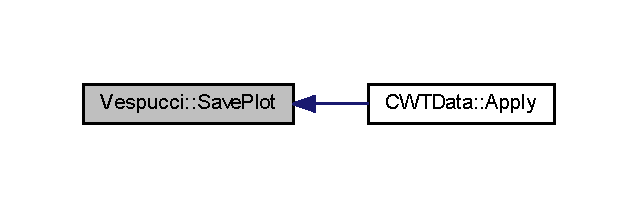
\includegraphics[width=306pt]{namespace_vespucci_ac9e75378ca4f326d27765420a5fe0017_icgraph}
\end{center}
\end{figure}


\hypertarget{namespace_vespucci_aa3b7c327a9c8fefe9f90b596b0522769}{\index{Vespucci@{Vespucci}!Set\+Q\+C\+P\+Fonts@{Set\+Q\+C\+P\+Fonts}}
\index{Set\+Q\+C\+P\+Fonts@{Set\+Q\+C\+P\+Fonts}!Vespucci@{Vespucci}}
\subsubsection[{Set\+Q\+C\+P\+Fonts}]{\setlength{\rightskip}{0pt plus 5cm}void Vespucci\+::\+Set\+Q\+C\+P\+Fonts (
\begin{DoxyParamCaption}
\item[{Q\+Custom\+Plot $\ast$}]{plot, }
\item[{const Q\+Font \&}]{font}
\end{DoxyParamCaption}
)}}\label{namespace_vespucci_aa3b7c327a9c8fefe9f90b596b0522769}


\hyperlink{namespace_vespucci_aa3b7c327a9c8fefe9f90b596b0522769}{Vespucci\+::\+Set\+Q\+C\+P\+Fonts}. 


\begin{DoxyParams}{Parameters}
{\em plot} & \\
\hline
{\em font} & \\
\hline
\end{DoxyParams}


Definition at line 127 of file vespucci.\+cpp.


\hypertarget{namespace_vespucci_1_1_math}{\section{Vespucci\+:\+:Math Namespace Reference}
\label{namespace_vespucci_1_1_math}\index{Vespucci\+::\+Math@{Vespucci\+::\+Math}}
}


A namespace for math functions relating to linear least squares regression.  


\subsection*{Namespaces}
\begin{DoxyCompactItemize}
\item 
 \hyperlink{namespace_vespucci_1_1_math_1_1_dimension_reduction}{Dimension\+Reduction}
\begin{DoxyCompactList}\small\item\em A namespace for math functions relating to dimension reduction. \end{DoxyCompactList}\item 
 \hyperlink{namespace_vespucci_1_1_math_1_1_fitting}{Fitting}
\begin{DoxyCompactList}\small\item\em A namespace for math functions relating to non-\/linear curve fitting. \end{DoxyCompactList}\item 
 \hyperlink{namespace_vespucci_1_1_math_1_1_normalization}{Normalization}
\begin{DoxyCompactList}\small\item\em A namespace for math functions relating to normalization. \end{DoxyCompactList}\item 
 \hyperlink{namespace_vespucci_1_1_math_1_1_peak_finding}{Peak\+Finding}
\begin{DoxyCompactList}\small\item\em A namespace for math functions relating to peak detection and counting. \end{DoxyCompactList}\item 
 \hyperlink{namespace_vespucci_1_1_math_1_1_quantification}{Quantification}
\begin{DoxyCompactList}\small\item\em A namespace for math functions relating to peak quantification. \end{DoxyCompactList}\item 
 \hyperlink{namespace_vespucci_1_1_math_1_1_smoothing}{Smoothing}
\begin{DoxyCompactList}\small\item\em A namespace for math functions relating to filtering and smoothing signals. \end{DoxyCompactList}\end{DoxyCompactItemize}
\subsection*{Classes}
\begin{DoxyCompactItemize}
\item 
class \hyperlink{class_vespucci_1_1_math_1_1_c_w_t_ridge}{C\+W\+T\+Ridge}
\end{DoxyCompactItemize}
\subsection*{Functions}
\begin{DoxyCompactItemize}
\item 
arma\+::sp\+\_\+mat \hyperlink{namespace_vespucci_1_1_math_a0ae415aafa638d49a2ee5b2816bdf7ec}{Local\+Maxima} (const arma\+::mat \&X)
\begin{DoxyCompactList}\small\item\em \hyperlink{namespace_vespucci_1_1_math_a0ae415aafa638d49a2ee5b2816bdf7ec}{Vespucci\+::\+Math\+::\+Local\+Maxima}. \end{DoxyCompactList}\item 
arma\+::sp\+\_\+mat \hyperlink{namespace_vespucci_1_1_math_ae5214109e423583abf4dfa8c71223343}{Local\+Maxima} (const arma\+::mat \&X, const arma\+::mat \&d\+X, const arma\+::mat \&d2\+X)
\begin{DoxyCompactList}\small\item\em \hyperlink{namespace_vespucci_1_1_math_a0ae415aafa638d49a2ee5b2816bdf7ec}{Vespucci\+::\+Math\+::\+Local\+Maxima}. \end{DoxyCompactList}\item 
\hypertarget{namespace_vespucci_1_1_math_a1422b7165b9083556e665f6bd9bf436f}{arma\+::sp\+\_\+mat {\bfseries Local\+Maxima} (const arma\+::mat \&d\+X, const arma\+::mat \&d2\+X)}\label{namespace_vespucci_1_1_math_a1422b7165b9083556e665f6bd9bf436f}

\item 
\hypertarget{namespace_vespucci_1_1_math_a72d209bf07859fa53f1f6aadf1d0a37b}{arma\+::sp\+\_\+mat {\bfseries Local\+Minima} (const arma\+::mat \&X)}\label{namespace_vespucci_1_1_math_a72d209bf07859fa53f1f6aadf1d0a37b}

\item 
\hypertarget{namespace_vespucci_1_1_math_ab06ee701a990bd32f2a635a85b8ea169}{arma\+::sp\+\_\+mat {\bfseries Local\+Minima} (const arma\+::mat \&X, const arma\+::mat \&d\+X, const arma\+::mat \&d2\+X)}\label{namespace_vespucci_1_1_math_ab06ee701a990bd32f2a635a85b8ea169}

\item 
\hypertarget{namespace_vespucci_1_1_math_a8d9d570bd9573eed29637015ea97a70f}{arma\+::sp\+\_\+mat {\bfseries Local\+Minima} (const arma\+::mat \&d\+X, const arma\+::mat \&d2\+X)}\label{namespace_vespucci_1_1_math_a8d9d570bd9573eed29637015ea97a70f}

\item 
\hypertarget{namespace_vespucci_1_1_math_a4c8faf974f4645faf1ab8d7e481e942e}{arma\+::sp\+\_\+mat {\bfseries Local\+Maxima\+C\+W\+T} (arma\+::mat coefs, arma\+::uvec scales, arma\+::uword min\+\_\+window\+\_\+size, double amplitude\+\_\+threshold)}\label{namespace_vespucci_1_1_math_a4c8faf974f4645faf1ab8d7e481e942e}

\item 
\hypertarget{namespace_vespucci_1_1_math_ae68dc0148a7d71a4d8fc32d5bb529fe2}{double {\bfseries quantile} (arma\+::vec \&data, double probs)}\label{namespace_vespucci_1_1_math_ae68dc0148a7d71a4d8fc32d5bb529fe2}

\item 
\hypertarget{namespace_vespucci_1_1_math_a969400e80b9f6bd1adf47db14cf4e38b}{double {\bfseries mad} (arma\+::vec \&data)}\label{namespace_vespucci_1_1_math_a969400e80b9f6bd1adf47db14cf4e38b}

\item 
\hypertarget{namespace_vespucci_1_1_math_aadc2b81e01a65a5de688088ca41791ce}{arma\+::vec {\bfseries Extend\+To\+Next\+Pow} (arma\+::vec X, arma\+::uword n)}\label{namespace_vespucci_1_1_math_aadc2b81e01a65a5de688088ca41791ce}

\item 
\hypertarget{namespace_vespucci_1_1_math_a979122c285b76d99e1cc430f8cd2fcd6}{arma\+::uword {\bfseries Next\+Pow} (arma\+::uword number, arma\+::uword power)}\label{namespace_vespucci_1_1_math_a979122c285b76d99e1cc430f8cd2fcd6}

\item 
arma\+::mat \hyperlink{namespace_vespucci_1_1_math_a3fecba29812be11a79fe7d9a2a88964e}{spdiags} (arma\+::mat B, arma\+::ivec d, arma\+::uword m, arma\+::uword n)
\begin{DoxyCompactList}\small\item\em spdiags analgous to the Octave/arma\+::mat\+L\+A\+B function A = spdiags(\+B, d, m, n). \end{DoxyCompactList}\item 
arma\+::mat \hyperlink{namespace_vespucci_1_1_math_a9ae51093bbdcdae2b8e6772d8951889c}{orth} (arma\+::mat X)
\begin{DoxyCompactList}\small\item\em orth Returns an orthonormal basis of the range space of A \end{DoxyCompactList}\item 
arma\+::uword \hyperlink{namespace_vespucci_1_1_math_a884dc00603c6aed8e2ee23988c429c64}{min} (arma\+::uword a, arma\+::uword b)
\begin{DoxyCompactList}\small\item\em \hyperlink{namespace_vespucci_1_1_math_a884dc00603c6aed8e2ee23988c429c64}{Vespucci\+::\+Math\+::min}. \end{DoxyCompactList}\item 
arma\+::uword \hyperlink{namespace_vespucci_1_1_math_a3d8f536b4465a4bacce89a51e3854daf}{max} (arma\+::uword a, arma\+::uword b)
\begin{DoxyCompactList}\small\item\em \hyperlink{namespace_vespucci_1_1_math_a3d8f536b4465a4bacce89a51e3854daf}{Vespucci\+::\+Math\+::max}. \end{DoxyCompactList}\item 
void \hyperlink{namespace_vespucci_1_1_math_a62f5e835cad1e15513494a5a48e028ae}{position} (arma\+::uword index, arma\+::uword n\+\_\+rows, arma\+::uword n\+\_\+cols, arma\+::uword \&i, arma\+::uword \&j)
\begin{DoxyCompactList}\small\item\em \hyperlink{namespace_vespucci_1_1_math_a62f5e835cad1e15513494a5a48e028ae}{Vespucci\+::\+Math\+::position} Find row and column numbers for index. \end{DoxyCompactList}\item 
\hypertarget{namespace_vespucci_1_1_math_a114f5bdc75f1c911ccf1d6e8652d6cfa}{arma\+::umat {\bfseries to\+\_\+row\+\_\+column} (arma\+::uvec indices, arma\+::uword n\+\_\+rows, arma\+::uword n\+\_\+cols)}\label{namespace_vespucci_1_1_math_a114f5bdc75f1c911ccf1d6e8652d6cfa}

\item 
double \hyperlink{namespace_vespucci_1_1_math_acb3549757968bb5b450a79ffce951cad}{Recalculate\+Average} (double new\+\_\+value, double old\+\_\+average, double old\+\_\+count)
\begin{DoxyCompactList}\small\item\em \hyperlink{namespace_vespucci_1_1_math_acb3549757968bb5b450a79ffce951cad}{Vespucci\+::\+Math\+::\+Recalculate\+Average} Recalculate the average value when a new value is added to a list for which only the previous means, stddevs and counts are known. \end{DoxyCompactList}\item 
double \hyperlink{namespace_vespucci_1_1_math_ab450596ed05ccd89c5183bd57ed1a0af}{Recalculate\+Std\+Dev} (double new\+\_\+value, double old\+\_\+mean, double old\+\_\+stddev, double old\+\_\+count)
\begin{DoxyCompactList}\small\item\em \hyperlink{namespace_vespucci_1_1_math_ab450596ed05ccd89c5183bd57ed1a0af}{Vespucci\+::\+Math\+::\+Recalculate\+Std\+Dev} Recalculate a standard deviation when a new value is added to a list for which only the previous means, stddevs and counts are known. \end{DoxyCompactList}\item 
\hypertarget{namespace_vespucci_1_1_math_a9c2b0dceba939de8417c1aa0382f9265}{{\footnotesize template$<$typename T $>$ }\\T {\bfseries conv\+\_\+fft} (const T \&A, const T \&B, std\+::string type)}\label{namespace_vespucci_1_1_math_a9c2b0dceba939de8417c1aa0382f9265}

\item 
\hypertarget{namespace_vespucci_1_1_math_a7928f8156c95fd307e7af5fef42bd2d0}{{\footnotesize template$<$typename T $>$ }\\T {\bfseries rotate} (const T \&X, arma\+::uword shift\+\_\+by, bool slide\+\_\+back=true)}\label{namespace_vespucci_1_1_math_a7928f8156c95fd307e7af5fef42bd2d0}

\item 
{\footnotesize template$<$typename T $>$ }\\T \hyperlink{namespace_vespucci_1_1_math_a9b57c78d676716cd14f45f1ed4cf066e}{diff} (const T \&X, arma\+::uword deriv\+\_\+order=1)
\begin{DoxyCompactList}\small\item\em \hyperlink{namespace_vespucci_1_1_math_a9b57c78d676716cd14f45f1ed4cf066e}{Vespucci\+::\+Math\+::diff}. \end{DoxyCompactList}\end{DoxyCompactItemize}


\subsection{Detailed Description}
A namespace for math functions relating to linear least squares regression. 

A namespace for math functions.

\+:\+::\+Lin\+Least\+Sq 

\subsection{Function Documentation}
\hypertarget{namespace_vespucci_1_1_math_a9b57c78d676716cd14f45f1ed4cf066e}{\index{Vespucci\+::\+Math@{Vespucci\+::\+Math}!diff@{diff}}
\index{diff@{diff}!Vespucci\+::\+Math@{Vespucci\+::\+Math}}
\subsubsection[{diff}]{\setlength{\rightskip}{0pt plus 5cm}template$<$typename T $>$ T Vespucci\+::\+Math\+::diff (
\begin{DoxyParamCaption}
\item[{const T \&}]{X, }
\item[{arma\+::uword}]{deriv\+\_\+order = {\ttfamily 1}}
\end{DoxyParamCaption}
)}}\label{namespace_vespucci_1_1_math_a9b57c78d676716cd14f45f1ed4cf066e}


\hyperlink{namespace_vespucci_1_1_math_a9b57c78d676716cd14f45f1ed4cf066e}{Vespucci\+::\+Math\+::diff}. 


\begin{DoxyParams}{Parameters}
{\em X} & A vector represetning a signal or a arma\+::matrix where each column is a signal \\
\hline
{\em deriv\+\_\+order} & The derivative order to calculate \\
\hline
\end{DoxyParams}
\begin{DoxyReturn}{Returns}
The deriv\+\_\+order-\/th derivative of X, a vector with deriv\+\_\+order fewer elements than X.
\end{DoxyReturn}
Perform arithmetic differentiation of a vector or arma\+::matrix (if X is a arma\+::matrix, the differentiation is performed to all the columns). 

Definition at line 46 of file accessory\+\_\+impl.\+h.



Here is the call graph for this function\+:
\nopagebreak
\begin{figure}[H]
\begin{center}
\leavevmode
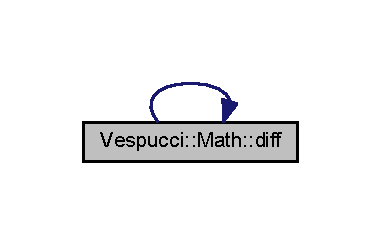
\includegraphics[width=183pt]{namespace_vespucci_1_1_math_a9b57c78d676716cd14f45f1ed4cf066e_cgraph}
\end{center}
\end{figure}




Here is the caller graph for this function\+:
\nopagebreak
\begin{figure}[H]
\begin{center}
\leavevmode
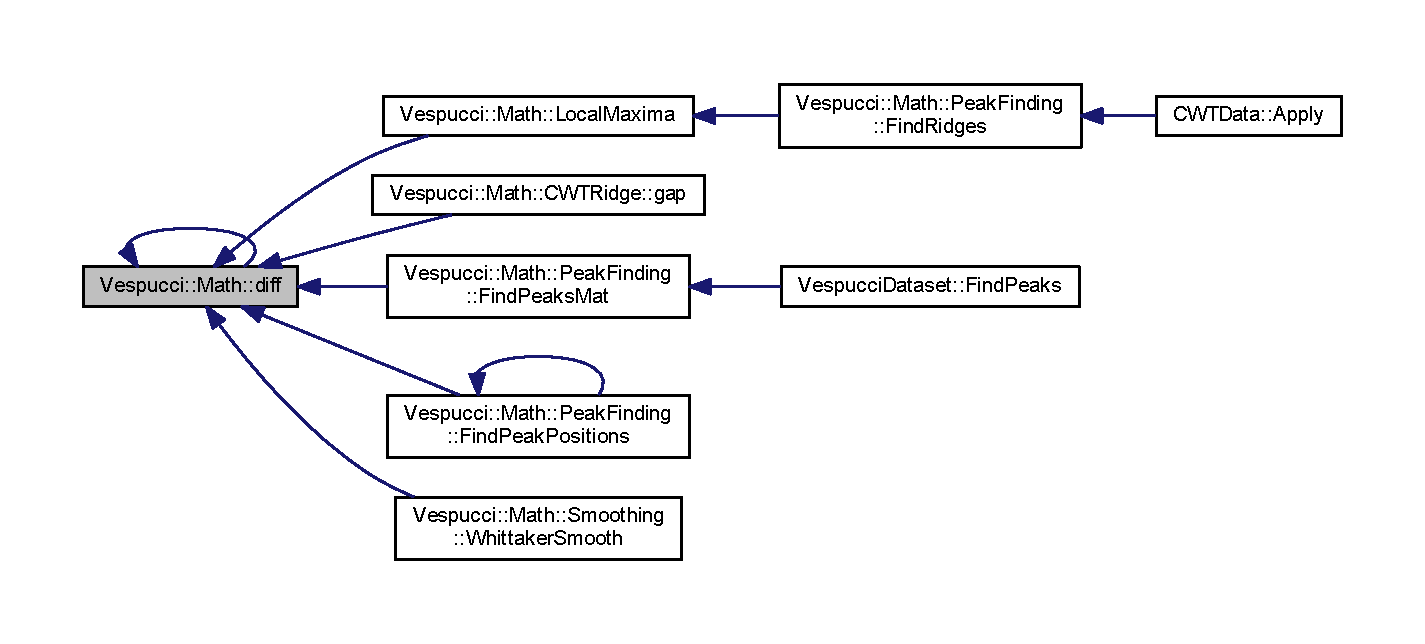
\includegraphics[width=350pt]{namespace_vespucci_1_1_math_a9b57c78d676716cd14f45f1ed4cf066e_icgraph}
\end{center}
\end{figure}


\hypertarget{namespace_vespucci_1_1_math_a0ae415aafa638d49a2ee5b2816bdf7ec}{\index{Vespucci\+::\+Math@{Vespucci\+::\+Math}!Local\+Maxima@{Local\+Maxima}}
\index{Local\+Maxima@{Local\+Maxima}!Vespucci\+::\+Math@{Vespucci\+::\+Math}}
\subsubsection[{Local\+Maxima}]{\setlength{\rightskip}{0pt plus 5cm}arma\+::sp\+\_\+mat Vespucci\+::\+Math\+::\+Local\+Maxima (
\begin{DoxyParamCaption}
\item[{const arma\+::mat \&}]{X}
\end{DoxyParamCaption}
)}}\label{namespace_vespucci_1_1_math_a0ae415aafa638d49a2ee5b2816bdf7ec}


\hyperlink{namespace_vespucci_1_1_math_a0ae415aafa638d49a2ee5b2816bdf7ec}{Vespucci\+::\+Math\+::\+Local\+Maxima}. 


\begin{DoxyParams}{Parameters}
{\em X} & A matrix with signals as columns \\
\hline
\end{DoxyParams}
\begin{DoxyReturn}{Returns}
A sparse matrix containing the value of each local maximum at the appropriate position. Find the local maxima of a matrix of signals using the first and second derivative tests. Works best with smooth signals (like C\+W\+T coeffs) 
\end{DoxyReturn}


Definition at line 191 of file accessory.\+cpp.



Here is the call graph for this function\+:
\nopagebreak
\begin{figure}[H]
\begin{center}
\leavevmode
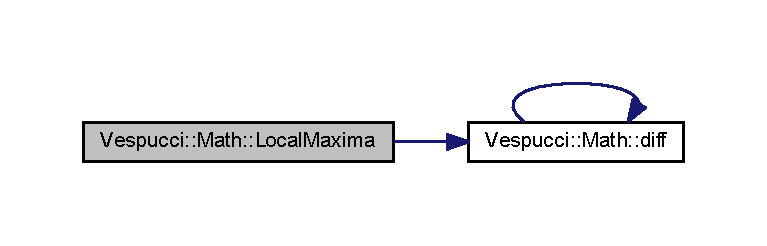
\includegraphics[width=350pt]{namespace_vespucci_1_1_math_a0ae415aafa638d49a2ee5b2816bdf7ec_cgraph}
\end{center}
\end{figure}




Here is the caller graph for this function\+:
\nopagebreak
\begin{figure}[H]
\begin{center}
\leavevmode
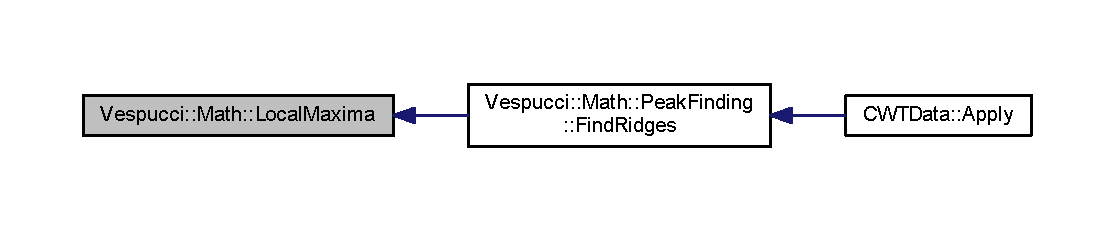
\includegraphics[width=350pt]{namespace_vespucci_1_1_math_a0ae415aafa638d49a2ee5b2816bdf7ec_icgraph}
\end{center}
\end{figure}


\hypertarget{namespace_vespucci_1_1_math_ae5214109e423583abf4dfa8c71223343}{\index{Vespucci\+::\+Math@{Vespucci\+::\+Math}!Local\+Maxima@{Local\+Maxima}}
\index{Local\+Maxima@{Local\+Maxima}!Vespucci\+::\+Math@{Vespucci\+::\+Math}}
\subsubsection[{Local\+Maxima}]{\setlength{\rightskip}{0pt plus 5cm}arma\+::sp\+\_\+mat Vespucci\+::\+Math\+::\+Local\+Maxima (
\begin{DoxyParamCaption}
\item[{const arma\+::mat \&}]{X, }
\item[{const arma\+::mat \&}]{d\+X, }
\item[{const arma\+::mat \&}]{d2\+X}
\end{DoxyParamCaption}
)}}\label{namespace_vespucci_1_1_math_ae5214109e423583abf4dfa8c71223343}


\hyperlink{namespace_vespucci_1_1_math_a0ae415aafa638d49a2ee5b2816bdf7ec}{Vespucci\+::\+Math\+::\+Local\+Maxima}. 


\begin{DoxyParams}{Parameters}
{\em X} & A matrix of signals \\
\hline
{\em d\+X} & A matrix of first derivatives of signals (numerical, S-\/\+G, wavelet, etc) \\
\hline
{\em d2\+X} & A matrix of second derivatives of signals (numerical, S-\/\+G, wavelet, etc). \\
\hline
\end{DoxyParams}
\begin{DoxyReturn}{Returns}

\end{DoxyReturn}


Definition at line 214 of file accessory.\+cpp.

\hypertarget{namespace_vespucci_1_1_math_a3d8f536b4465a4bacce89a51e3854daf}{\index{Vespucci\+::\+Math@{Vespucci\+::\+Math}!max@{max}}
\index{max@{max}!Vespucci\+::\+Math@{Vespucci\+::\+Math}}
\subsubsection[{max}]{\setlength{\rightskip}{0pt plus 5cm}arma\+::uword Vespucci\+::\+Math\+::max (
\begin{DoxyParamCaption}
\item[{arma\+::uword}]{a, }
\item[{arma\+::uword}]{b}
\end{DoxyParamCaption}
)}}\label{namespace_vespucci_1_1_math_a3d8f536b4465a4bacce89a51e3854daf}


\hyperlink{namespace_vespucci_1_1_math_a3d8f536b4465a4bacce89a51e3854daf}{Vespucci\+::\+Math\+::max}. 


\begin{DoxyParams}{Parameters}
{\em a} & \\
\hline
{\em b} & \\
\hline
\end{DoxyParams}
\begin{DoxyReturn}{Returns}
std\+::max stopped working with arma\+::uwords for some reason, so I made a max function It might be a better idea to just cast uwords to int and use std\+::max 
\end{DoxyReturn}


Definition at line 134 of file accessory.\+cpp.



Here is the caller graph for this function\+:
\nopagebreak
\begin{figure}[H]
\begin{center}
\leavevmode
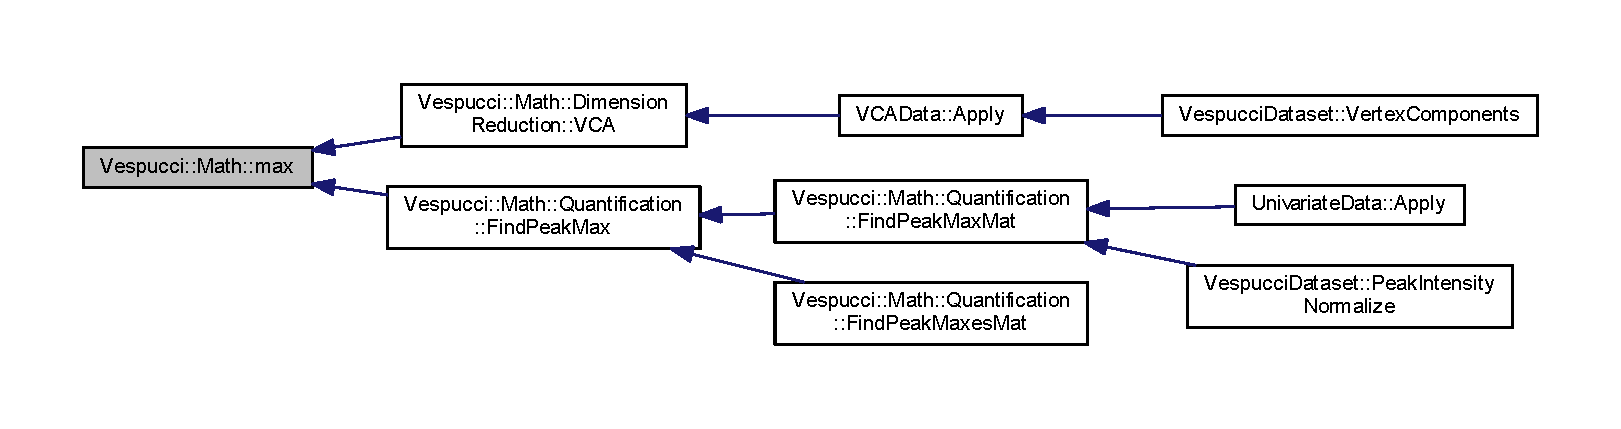
\includegraphics[width=350pt]{namespace_vespucci_1_1_math_a3d8f536b4465a4bacce89a51e3854daf_icgraph}
\end{center}
\end{figure}


\hypertarget{namespace_vespucci_1_1_math_a884dc00603c6aed8e2ee23988c429c64}{\index{Vespucci\+::\+Math@{Vespucci\+::\+Math}!min@{min}}
\index{min@{min}!Vespucci\+::\+Math@{Vespucci\+::\+Math}}
\subsubsection[{min}]{\setlength{\rightskip}{0pt plus 5cm}arma\+::uword Vespucci\+::\+Math\+::min (
\begin{DoxyParamCaption}
\item[{arma\+::uword}]{a, }
\item[{arma\+::uword}]{b}
\end{DoxyParamCaption}
)}}\label{namespace_vespucci_1_1_math_a884dc00603c6aed8e2ee23988c429c64}


\hyperlink{namespace_vespucci_1_1_math_a884dc00603c6aed8e2ee23988c429c64}{Vespucci\+::\+Math\+::min}. 


\begin{DoxyParams}{Parameters}
{\em a} & \\
\hline
{\em b} & \\
\hline
\end{DoxyParams}
\begin{DoxyReturn}{Returns}
std\+::min stopped working with arma\+::uwords for some reason, so I made a min function It might be a better idea to just cast uwords to int and use std\+::min 
\end{DoxyReturn}


Definition at line 146 of file accessory.\+cpp.

\hypertarget{namespace_vespucci_1_1_math_a9ae51093bbdcdae2b8e6772d8951889c}{\index{Vespucci\+::\+Math@{Vespucci\+::\+Math}!orth@{orth}}
\index{orth@{orth}!Vespucci\+::\+Math@{Vespucci\+::\+Math}}
\subsubsection[{orth}]{\setlength{\rightskip}{0pt plus 5cm}arma\+::mat Vespucci\+::\+Math\+::orth (
\begin{DoxyParamCaption}
\item[{arma\+::mat}]{X}
\end{DoxyParamCaption}
)}}\label{namespace_vespucci_1_1_math_a9ae51093bbdcdae2b8e6772d8951889c}


orth Returns an orthonormal basis of the range space of A 


\begin{DoxyParams}{Parameters}
{\em X} & arma\+::matrix \\
\hline
\end{DoxyParams}
\begin{DoxyReturn}{Returns}
a arma\+::matrix whose columns form an orthonormal basis for X This function was written before M\+L\+P\+A\+C\+K was used. The M\+L\+P\+A\+C\+K method mlpack\+::math\+::\+Orthogonalize does the same thing 
\end{DoxyReturn}


Definition at line 104 of file accessory.\+cpp.

\hypertarget{namespace_vespucci_1_1_math_a62f5e835cad1e15513494a5a48e028ae}{\index{Vespucci\+::\+Math@{Vespucci\+::\+Math}!position@{position}}
\index{position@{position}!Vespucci\+::\+Math@{Vespucci\+::\+Math}}
\subsubsection[{position}]{\setlength{\rightskip}{0pt plus 5cm}void Vespucci\+::\+Math\+::position (
\begin{DoxyParamCaption}
\item[{arma\+::uword}]{index, }
\item[{arma\+::uword}]{n\+\_\+rows, }
\item[{arma\+::uword}]{n\+\_\+cols, }
\item[{arma\+::uword \&}]{i, }
\item[{arma\+::uword \&}]{j}
\end{DoxyParamCaption}
)}}\label{namespace_vespucci_1_1_math_a62f5e835cad1e15513494a5a48e028ae}


\hyperlink{namespace_vespucci_1_1_math_a62f5e835cad1e15513494a5a48e028ae}{Vespucci\+::\+Math\+::position} Find row and column numbers for index. 


\begin{DoxyParams}{Parameters}
{\em index} & \\
\hline
{\em n\+\_\+rows} & Number of rows \\
\hline
{\em n\+\_\+cols} & Number of columns \\
\hline
{\em i} & Row number \\
\hline
{\em j} & Column number \\
\hline
\end{DoxyParams}


Definition at line 355 of file accessory.\+cpp.



Here is the caller graph for this function\+:
\nopagebreak
\begin{figure}[H]
\begin{center}
\leavevmode
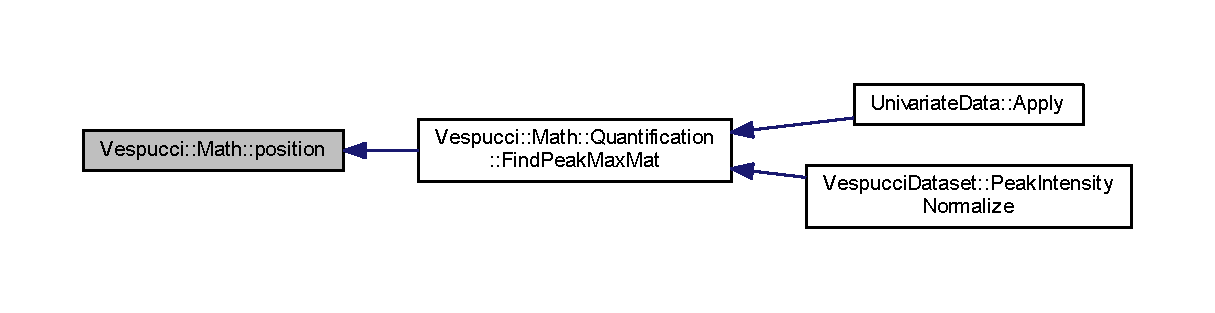
\includegraphics[width=350pt]{namespace_vespucci_1_1_math_a62f5e835cad1e15513494a5a48e028ae_icgraph}
\end{center}
\end{figure}


\hypertarget{namespace_vespucci_1_1_math_acb3549757968bb5b450a79ffce951cad}{\index{Vespucci\+::\+Math@{Vespucci\+::\+Math}!Recalculate\+Average@{Recalculate\+Average}}
\index{Recalculate\+Average@{Recalculate\+Average}!Vespucci\+::\+Math@{Vespucci\+::\+Math}}
\subsubsection[{Recalculate\+Average}]{\setlength{\rightskip}{0pt plus 5cm}double Vespucci\+::\+Math\+::\+Recalculate\+Average (
\begin{DoxyParamCaption}
\item[{double}]{new\+\_\+value, }
\item[{double}]{old\+\_\+average, }
\item[{double}]{old\+\_\+count}
\end{DoxyParamCaption}
)}}\label{namespace_vespucci_1_1_math_acb3549757968bb5b450a79ffce951cad}


\hyperlink{namespace_vespucci_1_1_math_acb3549757968bb5b450a79ffce951cad}{Vespucci\+::\+Math\+::\+Recalculate\+Average} Recalculate the average value when a new value is added to a list for which only the previous means, stddevs and counts are known. 


\begin{DoxyParams}{Parameters}
{\em new\+\_\+value} & \\
\hline
{\em old\+\_\+average} & \\
\hline
{\em old\+\_\+count} & \\
\hline
\end{DoxyParams}
\begin{DoxyReturn}{Returns}

\end{DoxyReturn}


Definition at line 452 of file accessory.\+cpp.



Here is the caller graph for this function\+:
\nopagebreak
\begin{figure}[H]
\begin{center}
\leavevmode
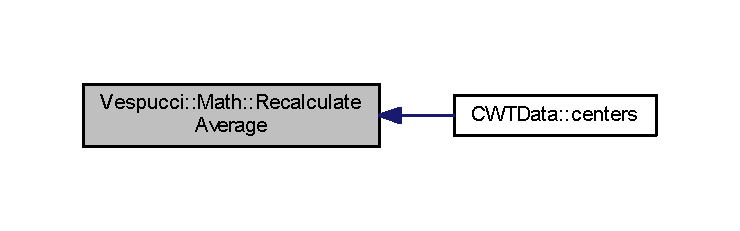
\includegraphics[width=350pt]{namespace_vespucci_1_1_math_acb3549757968bb5b450a79ffce951cad_icgraph}
\end{center}
\end{figure}


\hypertarget{namespace_vespucci_1_1_math_ab450596ed05ccd89c5183bd57ed1a0af}{\index{Vespucci\+::\+Math@{Vespucci\+::\+Math}!Recalculate\+Std\+Dev@{Recalculate\+Std\+Dev}}
\index{Recalculate\+Std\+Dev@{Recalculate\+Std\+Dev}!Vespucci\+::\+Math@{Vespucci\+::\+Math}}
\subsubsection[{Recalculate\+Std\+Dev}]{\setlength{\rightskip}{0pt plus 5cm}double Vespucci\+::\+Math\+::\+Recalculate\+Std\+Dev (
\begin{DoxyParamCaption}
\item[{double}]{new\+\_\+value, }
\item[{double}]{old\+\_\+mean, }
\item[{double}]{old\+\_\+stddev, }
\item[{double}]{old\+\_\+count}
\end{DoxyParamCaption}
)}}\label{namespace_vespucci_1_1_math_ab450596ed05ccd89c5183bd57ed1a0af}


\hyperlink{namespace_vespucci_1_1_math_ab450596ed05ccd89c5183bd57ed1a0af}{Vespucci\+::\+Math\+::\+Recalculate\+Std\+Dev} Recalculate a standard deviation when a new value is added to a list for which only the previous means, stddevs and counts are known. 


\begin{DoxyParams}{Parameters}
{\em new\+\_\+value} & \\
\hline
{\em old\+\_\+mean} & \\
\hline
{\em old\+\_\+stddev} & \\
\hline
{\em old\+\_\+count} & \\
\hline
\end{DoxyParams}
\begin{DoxyReturn}{Returns}

\end{DoxyReturn}


Definition at line 469 of file accessory.\+cpp.



Here is the caller graph for this function\+:
\nopagebreak
\begin{figure}[H]
\begin{center}
\leavevmode
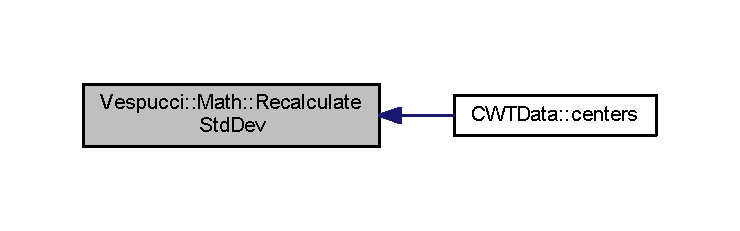
\includegraphics[width=350pt]{namespace_vespucci_1_1_math_ab450596ed05ccd89c5183bd57ed1a0af_icgraph}
\end{center}
\end{figure}


\hypertarget{namespace_vespucci_1_1_math_a3fecba29812be11a79fe7d9a2a88964e}{\index{Vespucci\+::\+Math@{Vespucci\+::\+Math}!spdiags@{spdiags}}
\index{spdiags@{spdiags}!Vespucci\+::\+Math@{Vespucci\+::\+Math}}
\subsubsection[{spdiags}]{\setlength{\rightskip}{0pt plus 5cm}arma\+::mat Vespucci\+::\+Math\+::spdiags (
\begin{DoxyParamCaption}
\item[{arma\+::mat}]{B, }
\item[{arma\+::ivec}]{d, }
\item[{arma\+::uword}]{m, }
\item[{arma\+::uword}]{n}
\end{DoxyParamCaption}
)}}\label{namespace_vespucci_1_1_math_a3fecba29812be11a79fe7d9a2a88964e}


spdiags analgous to the Octave/arma\+::mat\+L\+A\+B function A = spdiags(\+B, d, m, n). 


\begin{DoxyParams}{Parameters}
{\em B} & a arma\+::matrix containing the new diagonal vectors as columns \\
\hline
{\em d} & a vector containing the row numbers to set. The first column vector of B corresponds to the first entry in d. \\
\hline
{\em m} & the number of rows of the output arma\+::matrix \\
\hline
{\em n} & the number of columns of the output arma\+::matrix \\
\hline
\end{DoxyParams}
\begin{DoxyReturn}{Returns}
a m by n sparase arma\+::matrix with the columns of B as diagonals A translation of the Octave/arma\+::mat\+L\+A\+B function A = spdiags(\+B, d, m, n). For subdiagonals (entries of d $<$ 0) vectors are truncated at the end when they are longer than the target diagonal. For superdiagonals, vectors are truncated at the beginning when they are longer than the target diagonal. 
\end{DoxyReturn}


Definition at line 33 of file accessory.\+cpp.


\hypertarget{namespace_vespucci_1_1_math_1_1_dimension_reduction}{\section{Vespucci\+:\+:Math\+:\+:Dimension\+Reduction Namespace Reference}
\label{namespace_vespucci_1_1_math_1_1_dimension_reduction}\index{Vespucci\+::\+Math\+::\+Dimension\+Reduction@{Vespucci\+::\+Math\+::\+Dimension\+Reduction}}
}


A namespace for math functions relating to dimension reduction.  


\subsection*{Functions}
\begin{DoxyCompactItemize}
\item 
bool \hyperlink{namespace_vespucci_1_1_math_1_1_dimension_reduction_a5878e156d2d744ee078a70eeb59f97b3}{plsregress} (arma\+::mat X, arma\+::mat Y, int components, arma\+::mat \&X\+\_\+loadings, arma\+::mat \&Y\+\_\+loadings, arma\+::mat \&X\+\_\+scores, arma\+::mat \&Y\+\_\+scores, arma\+::mat \&coefficients, arma\+::mat \&percent\+\_\+variance, arma\+::mat \&fitted)
\begin{DoxyCompactList}\small\item\em Vespucci\+::\+Math\+Dimension\+Reduction\+::plsregress P\+L\+S Regression Using S\+I\+M\+P\+L\+S algorithm. This is essentially a line-\/for-\/line rewrite of plsregress from the Octave statistics package. Copyright (C) 2012 Fernando Damian Nieuwveldt \href{mailto:fdnieuwveldt@gmail.com}{\tt fdnieuwveldt@gmail.\+com} This is an implementation of the S\+I\+M\+P\+L\+S algorithm\+: Reference\+: S\+I\+M\+P\+L\+S\+: An alternative approach to partial least squares regression. Chemometrics and Intelligent Laboratory Systems (1993) \end{DoxyCompactList}\item 
bool \hyperlink{namespace_vespucci_1_1_math_1_1_dimension_reduction_a2d46d5cccce427efee376aeeea2da058}{V\+C\+A} (const arma\+::mat \&R, arma\+::uword p, arma\+::uvec \&indices, arma\+::mat \&endmember\+\_\+spectra, arma\+::mat \&projected\+\_\+data, arma\+::mat \&fractional\+\_\+abundances)
\begin{DoxyCompactList}\small\item\em \hyperlink{namespace_vespucci_1_1_math_1_1_dimension_reduction_a2d46d5cccce427efee376aeeea2da058}{Vespucci\+::\+Math\+::\+Dimension\+Reduction\+::\+V\+C\+A} Vertex Component Analysis. \end{DoxyCompactList}\item 
double \hyperlink{namespace_vespucci_1_1_math_1_1_dimension_reduction_a37f3a4278bbdfba337f4e776f7d0916b}{estimate\+\_\+snr} (const arma\+::mat \&R, arma\+::vec r\+\_\+m, arma\+::mat x)
\begin{DoxyCompactList}\small\item\em \hyperlink{namespace_vespucci_1_1_math}{Vespucci\+::\+Math} Estimates Signal-\/to-\/\+Noise ratio. {\bfseries [Nascimento2005]}. \end{DoxyCompactList}\item 
int \hyperlink{namespace_vespucci_1_1_math_1_1_dimension_reduction_a355295f13e2a14e990b22eb96a33db5c}{Hy\+Sime} (arma\+::mat y, arma\+::mat n, arma\+::mat Rn, arma\+::mat \&Ek)
\begin{DoxyCompactList}\small\item\em \hyperlink{namespace_vespucci_1_1_math_1_1_dimension_reduction_a355295f13e2a14e990b22eb96a33db5c}{Vespucci\+::\+Math\+::\+Dimension\+Reduction\+::\+Hy\+Sime}. \end{DoxyCompactList}\item 
void \hyperlink{namespace_vespucci_1_1_math_1_1_dimension_reduction_ac96e3dc096295499724e3ecbb63a3f57}{Estimate\+Additive\+Noise} (arma\+::mat \&noise, arma\+::mat \&noise\+\_\+correlation, const arma\+::mat \&sample)
\begin{DoxyCompactList}\small\item\em \hyperlink{namespace_vespucci_1_1_math_1_1_dimension_reduction_ac96e3dc096295499724e3ecbb63a3f57}{Vespucci\+::\+Math\+::\+Dimension\+Reduction\+::\+Estimate\+Additive\+Noise}. \end{DoxyCompactList}\end{DoxyCompactItemize}


\subsection{Detailed Description}
A namespace for math functions relating to dimension reduction. 

A namespace for math functions relating to transforms. 

\subsection{Function Documentation}
\hypertarget{namespace_vespucci_1_1_math_1_1_dimension_reduction_a37f3a4278bbdfba337f4e776f7d0916b}{\index{Vespucci\+::\+Math\+::\+Dimension\+Reduction@{Vespucci\+::\+Math\+::\+Dimension\+Reduction}!estimate\+\_\+snr@{estimate\+\_\+snr}}
\index{estimate\+\_\+snr@{estimate\+\_\+snr}!Vespucci\+::\+Math\+::\+Dimension\+Reduction@{Vespucci\+::\+Math\+::\+Dimension\+Reduction}}
\subsubsection[{estimate\+\_\+snr}]{\setlength{\rightskip}{0pt plus 5cm}double Vespucci\+::\+Math\+::\+Dimension\+Reduction\+::estimate\+\_\+snr (
\begin{DoxyParamCaption}
\item[{const arma\+::mat \&}]{R, }
\item[{arma\+::vec}]{r\+\_\+m, }
\item[{arma\+::mat}]{x}
\end{DoxyParamCaption}
)}}\label{namespace_vespucci_1_1_math_1_1_dimension_reduction_a37f3a4278bbdfba337f4e776f7d0916b}


\hyperlink{namespace_vespucci_1_1_math}{Vespucci\+::\+Math} Estimates Signal-\/to-\/\+Noise ratio. {\bfseries [Nascimento2005]}. 


\begin{DoxyParams}{Parameters}
{\em R} & Input \\
\hline
{\em r\+\_\+m} & \\
\hline
{\em x} & \\
\hline
\end{DoxyParams}
\begin{DoxyReturn}{Returns}

\end{DoxyReturn}


Definition at line 126 of file V\+C\+A.\+cpp.



Here is the caller graph for this function\+:
\nopagebreak
\begin{figure}[H]
\begin{center}
\leavevmode
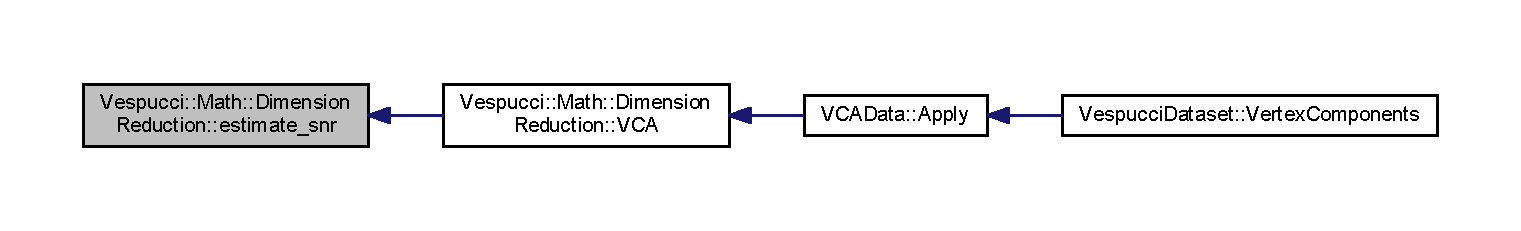
\includegraphics[width=350pt]{namespace_vespucci_1_1_math_1_1_dimension_reduction_a37f3a4278bbdfba337f4e776f7d0916b_icgraph}
\end{center}
\end{figure}


\hypertarget{namespace_vespucci_1_1_math_1_1_dimension_reduction_ac96e3dc096295499724e3ecbb63a3f57}{\index{Vespucci\+::\+Math\+::\+Dimension\+Reduction@{Vespucci\+::\+Math\+::\+Dimension\+Reduction}!Estimate\+Additive\+Noise@{Estimate\+Additive\+Noise}}
\index{Estimate\+Additive\+Noise@{Estimate\+Additive\+Noise}!Vespucci\+::\+Math\+::\+Dimension\+Reduction@{Vespucci\+::\+Math\+::\+Dimension\+Reduction}}
\subsubsection[{Estimate\+Additive\+Noise}]{\setlength{\rightskip}{0pt plus 5cm}void Vespucci\+::\+Math\+::\+Dimension\+Reduction\+::\+Estimate\+Additive\+Noise (
\begin{DoxyParamCaption}
\item[{arma\+::mat \&}]{noise, }
\item[{arma\+::mat \&}]{noise\+\_\+correlation, }
\item[{const arma\+::mat \&}]{sample}
\end{DoxyParamCaption}
)}}\label{namespace_vespucci_1_1_math_1_1_dimension_reduction_ac96e3dc096295499724e3ecbb63a3f57}


\hyperlink{namespace_vespucci_1_1_math_1_1_dimension_reduction_ac96e3dc096295499724e3ecbb63a3f57}{Vespucci\+::\+Math\+::\+Dimension\+Reduction\+::\+Estimate\+Additive\+Noise}. 


\begin{DoxyParams}{Parameters}
{\em noise} & \\
\hline
{\em noise\+\_\+correlation} & \\
\hline
{\em sample} & The slow additive noise mat\+::mator from the Hy\+Sime paper. I'm looking into faster ones. \\
\hline
\end{DoxyParams}


Definition at line 198 of file V\+C\+A.\+cpp.



Here is the caller graph for this function\+:
\nopagebreak
\begin{figure}[H]
\begin{center}
\leavevmode
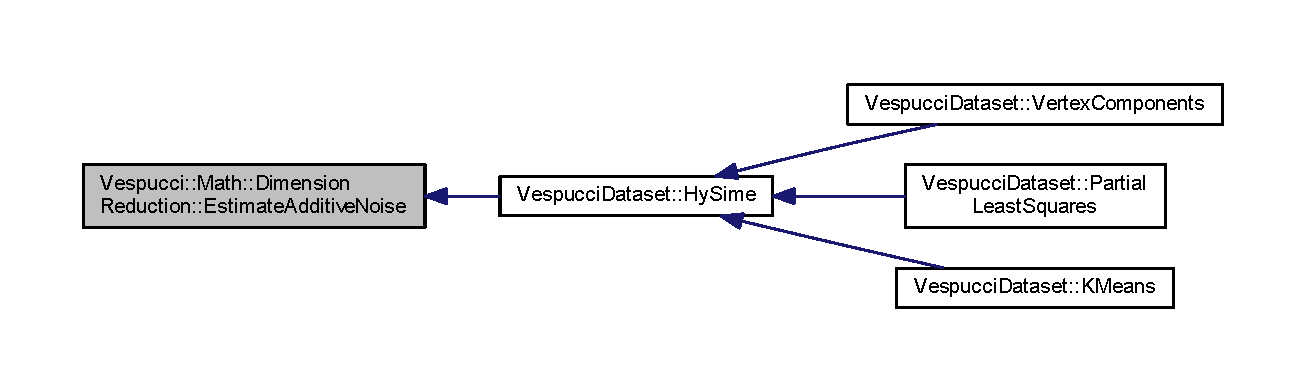
\includegraphics[width=350pt]{namespace_vespucci_1_1_math_1_1_dimension_reduction_ac96e3dc096295499724e3ecbb63a3f57_icgraph}
\end{center}
\end{figure}


\hypertarget{namespace_vespucci_1_1_math_1_1_dimension_reduction_a355295f13e2a14e990b22eb96a33db5c}{\index{Vespucci\+::\+Math\+::\+Dimension\+Reduction@{Vespucci\+::\+Math\+::\+Dimension\+Reduction}!Hy\+Sime@{Hy\+Sime}}
\index{Hy\+Sime@{Hy\+Sime}!Vespucci\+::\+Math\+::\+Dimension\+Reduction@{Vespucci\+::\+Math\+::\+Dimension\+Reduction}}
\subsubsection[{Hy\+Sime}]{\setlength{\rightskip}{0pt plus 5cm}int Vespucci\+::\+Math\+::\+Dimension\+Reduction\+::\+Hy\+Sime (
\begin{DoxyParamCaption}
\item[{arma\+::mat}]{y, }
\item[{arma\+::mat}]{n, }
\item[{arma\+::mat}]{Rn, }
\item[{arma\+::mat \&}]{Ek}
\end{DoxyParamCaption}
)}}\label{namespace_vespucci_1_1_math_1_1_dimension_reduction_a355295f13e2a14e990b22eb96a33db5c}


\hyperlink{namespace_vespucci_1_1_math_1_1_dimension_reduction_a355295f13e2a14e990b22eb96a33db5c}{Vespucci\+::\+Math\+::\+Dimension\+Reduction\+::\+Hy\+Sime}. 


\begin{DoxyParams}{Parameters}
{\em y} & \\
\hline
{\em n} & \\
\hline
{\em Rn} & \\
\hline
{\em Ek} & \\
\hline
\end{DoxyParams}
\begin{DoxyReturn}{Returns}
Performs the Hy\+Sime algorithm to predict the rank of y 
\end{DoxyReturn}


Definition at line 149 of file V\+C\+A.\+cpp.



Here is the caller graph for this function\+:
\nopagebreak
\begin{figure}[H]
\begin{center}
\leavevmode
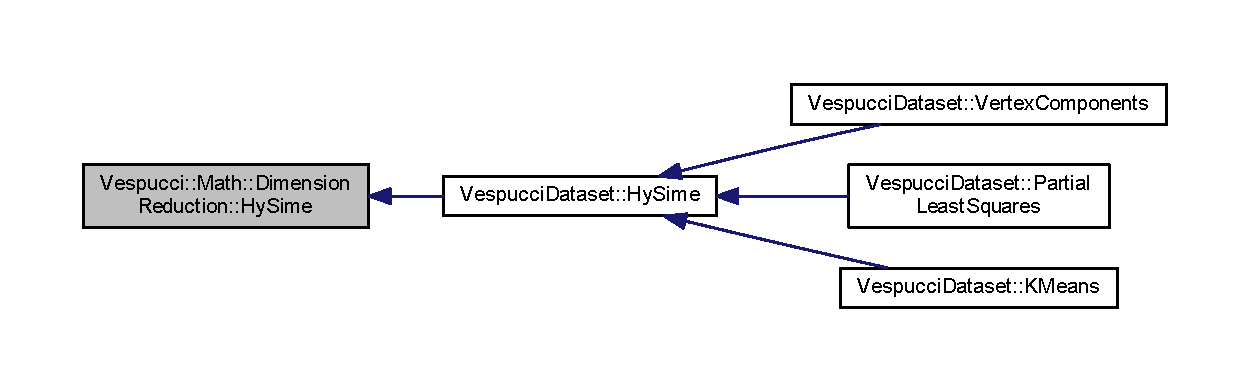
\includegraphics[width=350pt]{namespace_vespucci_1_1_math_1_1_dimension_reduction_a355295f13e2a14e990b22eb96a33db5c_icgraph}
\end{center}
\end{figure}


\hypertarget{namespace_vespucci_1_1_math_1_1_dimension_reduction_a5878e156d2d744ee078a70eeb59f97b3}{\index{Vespucci\+::\+Math\+::\+Dimension\+Reduction@{Vespucci\+::\+Math\+::\+Dimension\+Reduction}!plsregress@{plsregress}}
\index{plsregress@{plsregress}!Vespucci\+::\+Math\+::\+Dimension\+Reduction@{Vespucci\+::\+Math\+::\+Dimension\+Reduction}}
\subsubsection[{plsregress}]{\setlength{\rightskip}{0pt plus 5cm}bool Vespucci\+::\+Math\+::\+Dimension\+Reduction\+::plsregress (
\begin{DoxyParamCaption}
\item[{arma\+::mat}]{X, }
\item[{arma\+::mat}]{Y, }
\item[{int}]{components, }
\item[{arma\+::mat \&}]{X\+\_\+loadings, }
\item[{arma\+::mat \&}]{Y\+\_\+loadings, }
\item[{arma\+::mat \&}]{X\+\_\+scores, }
\item[{arma\+::mat \&}]{Y\+\_\+scores, }
\item[{arma\+::mat \&}]{coefficients, }
\item[{arma\+::mat \&}]{percent\+\_\+variance, }
\item[{arma\+::mat \&}]{fitted}
\end{DoxyParamCaption}
)}}\label{namespace_vespucci_1_1_math_1_1_dimension_reduction_a5878e156d2d744ee078a70eeb59f97b3}


Vespucci\+::\+Math\+Dimension\+Reduction\+::plsregress P\+L\+S Regression Using S\+I\+M\+P\+L\+S algorithm. This is essentially a line-\/for-\/line rewrite of plsregress from the Octave statistics package. Copyright (C) 2012 Fernando Damian Nieuwveldt \href{mailto:fdnieuwveldt@gmail.com}{\tt fdnieuwveldt@gmail.\+com} This is an implementation of the S\+I\+M\+P\+L\+S algorithm\+: Reference\+: S\+I\+M\+P\+L\+S\+: An alternative approach to partial least squares regression. Chemometrics and Intelligent Laboratory Systems (1993) 


\begin{DoxyParams}{Parameters}
{\em x} & \\
\hline
{\em y} & \\
\hline
{\em components} & Number of P\+L\+S components \\
\hline
{\em x\+\_\+loadings} & \char`\"{}\+Output\char`\"{} values \\
\hline
{\em y\+\_\+loadings} & \\
\hline
{\em x\+\_\+scores} & \\
\hline
{\em y\+\_\+scores} & \\
\hline
{\em coefficients} & \\
\hline
{\em fitted\+\_\+data} & \\
\hline
\end{DoxyParams}
\begin{DoxyReturn}{Returns}

\end{DoxyReturn}


Definition at line 41 of file pls.\+cpp.



Here is the caller graph for this function\+:
\nopagebreak
\begin{figure}[H]
\begin{center}
\leavevmode
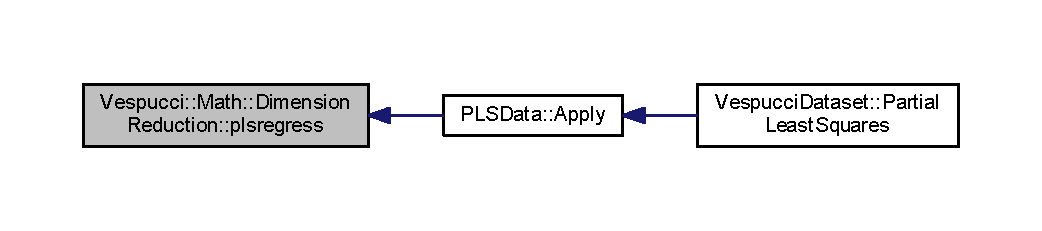
\includegraphics[width=350pt]{namespace_vespucci_1_1_math_1_1_dimension_reduction_a5878e156d2d744ee078a70eeb59f97b3_icgraph}
\end{center}
\end{figure}


\hypertarget{namespace_vespucci_1_1_math_1_1_dimension_reduction_a2d46d5cccce427efee376aeeea2da058}{\index{Vespucci\+::\+Math\+::\+Dimension\+Reduction@{Vespucci\+::\+Math\+::\+Dimension\+Reduction}!V\+C\+A@{V\+C\+A}}
\index{V\+C\+A@{V\+C\+A}!Vespucci\+::\+Math\+::\+Dimension\+Reduction@{Vespucci\+::\+Math\+::\+Dimension\+Reduction}}
\subsubsection[{V\+C\+A}]{\setlength{\rightskip}{0pt plus 5cm}bool Vespucci\+::\+Math\+::\+Dimension\+Reduction\+::\+V\+C\+A (
\begin{DoxyParamCaption}
\item[{const arma\+::mat \&}]{R, }
\item[{arma\+::uword}]{p, }
\item[{arma\+::uvec \&}]{indices, }
\item[{arma\+::mat \&}]{endmember\+\_\+spectra, }
\item[{arma\+::mat \&}]{projected\+\_\+data, }
\item[{arma\+::mat \&}]{fractional\+\_\+abundances}
\end{DoxyParamCaption}
)}}\label{namespace_vespucci_1_1_math_1_1_dimension_reduction_a2d46d5cccce427efee376aeeea2da058}


\hyperlink{namespace_vespucci_1_1_math_1_1_dimension_reduction_a2d46d5cccce427efee376aeeea2da058}{Vespucci\+::\+Math\+::\+Dimension\+Reduction\+::\+V\+C\+A} Vertex Component Analysis. 


\begin{DoxyParams}{Parameters}
{\em R} & The dataset \\
\hline
{\em endmembers} & Number of endmembers to compute \\
\hline
{\em indices} & Row indices of pure components. \\
\hline
{\em endmember\+\_\+spectra} & Spectra of pure components (note that these are in columns, not rows as in spectra\+\_\+) \\
\hline
{\em projected\+\_\+data} & Projected data \\
\hline
{\em fractional\+\_\+abundances} & Purity of a given spectrum relative to endmember \\
\hline
\end{DoxyParams}
\begin{DoxyReturn}{Returns}
Convergeance (no actual test implemented...) 
\end{DoxyReturn}


Definition at line 34 of file V\+C\+A.\+cpp.



Here is the call graph for this function\+:
\nopagebreak
\begin{figure}[H]
\begin{center}
\leavevmode
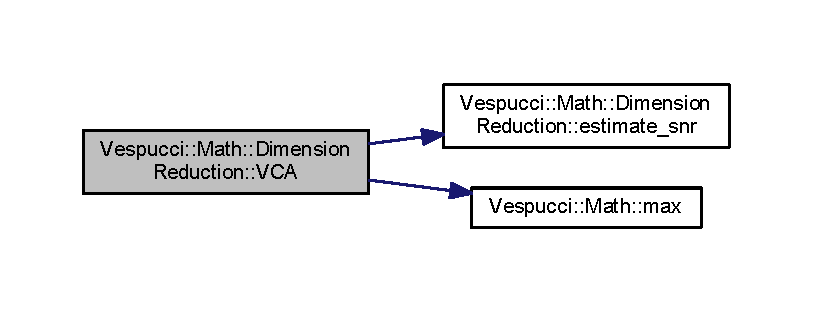
\includegraphics[width=350pt]{namespace_vespucci_1_1_math_1_1_dimension_reduction_a2d46d5cccce427efee376aeeea2da058_cgraph}
\end{center}
\end{figure}




Here is the caller graph for this function\+:
\nopagebreak
\begin{figure}[H]
\begin{center}
\leavevmode
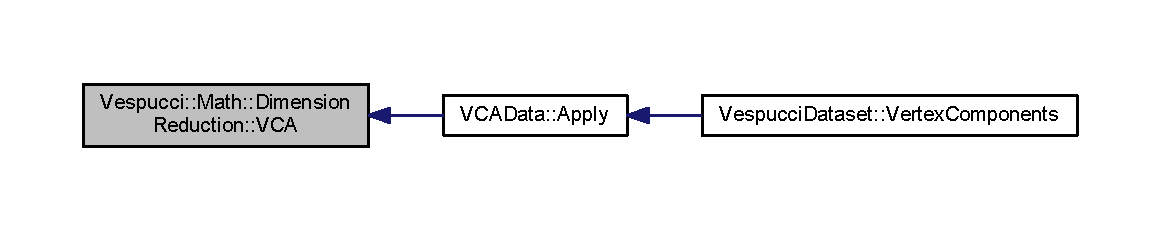
\includegraphics[width=350pt]{namespace_vespucci_1_1_math_1_1_dimension_reduction_a2d46d5cccce427efee376aeeea2da058_icgraph}
\end{center}
\end{figure}



\hypertarget{namespace_vespucci_1_1_math_1_1_fitting}{\section{Vespucci\+:\+:Math\+:\+:Fitting Namespace Reference}
\label{namespace_vespucci_1_1_math_1_1_fitting}\index{Vespucci\+::\+Math\+::\+Fitting@{Vespucci\+::\+Math\+::\+Fitting}}
}


A namespace for math functions relating to non-\/linear curve fitting.  


\subsection*{Functions}
\begin{DoxyCompactItemize}
\item 
\hypertarget{namespace_vespucci_1_1_math_1_1_fitting_a6a3b8f03530b331694b06842312ff706}{arma\+::vec {\bfseries Fit\+Baseline} (arma\+::vec signal, std\+::string function, std\+::vector$<$ double $>$ initial\+\_\+params, std\+::vector$<$ double $>$ lims)}\label{namespace_vespucci_1_1_math_1_1_fitting_a6a3b8f03530b331694b06842312ff706}

\item 
arma\+::vec \hyperlink{namespace_vespucci_1_1_math_1_1_fitting_a7ccac4eb07dd9eaa7c891e8d78be6390}{Fit\+Gaussian\+Peak} (arma\+::vec signal, int iterations, std\+::string \&reason, std\+::map$<$ std\+::string, std\+::pair$<$ double, double $>$ $>$ \&params, std\+::map$<$ std\+::string, double $>$ \&stats, arma\+::vec \&residuals)
\begin{DoxyCompactList}\small\item\em \hyperlink{namespace_vespucci_1_1_math_1_1_fitting_a7ccac4eb07dd9eaa7c891e8d78be6390}{Vespucci\+::\+Math\+::\+Fitting\+::\+Fit\+Gaussian\+Peak} fit a gaussian function to a vector using the Levenberg-\/\+Marquardt algorithm. \end{DoxyCompactList}\item 
\hypertarget{namespace_vespucci_1_1_math_1_1_fitting_ad882180a79f7fb8c0b82c655345c2089}{void {\bfseries Gaussian} (double $\ast$p, double $\ast$x, int m, int n, void $\ast$data)}\label{namespace_vespucci_1_1_math_1_1_fitting_ad882180a79f7fb8c0b82c655345c2089}

\item 
\hypertarget{namespace_vespucci_1_1_math_1_1_fitting_a13a109b0157d2715cba67fc5e6630505}{void {\bfseries Gaussian\+Jacobian} (double $\ast$p, double $\ast$jac, int m, int n, void $\ast$data)}\label{namespace_vespucci_1_1_math_1_1_fitting_a13a109b0157d2715cba67fc5e6630505}

\item 
\hypertarget{namespace_vespucci_1_1_math_1_1_fitting_ac720c74022d65f7f11b1b301842beebb}{void {\bfseries Lorentzian} (double $\ast$p, double $\ast$x, int m, int n, void $\ast$data)}\label{namespace_vespucci_1_1_math_1_1_fitting_ac720c74022d65f7f11b1b301842beebb}

\item 
\hypertarget{namespace_vespucci_1_1_math_1_1_fitting_a46da5c5db0cd303cd4b1e5831ca95ee8}{void {\bfseries Lorentzian\+Jacobian} (double $\ast$p, double $\ast$jac, int m, int n, void $\ast$data)}\label{namespace_vespucci_1_1_math_1_1_fitting_a46da5c5db0cd303cd4b1e5831ca95ee8}

\item 
\hypertarget{namespace_vespucci_1_1_math_1_1_fitting_a861a613f20ecc6d496c2eb06ec183e0a}{void {\bfseries Pseudo\+Voigt} (double $\ast$p, double $\ast$x, int m, int n, void $\ast$data)}\label{namespace_vespucci_1_1_math_1_1_fitting_a861a613f20ecc6d496c2eb06ec183e0a}

\item 
\hypertarget{namespace_vespucci_1_1_math_1_1_fitting_a9fbd24e3adec9a9da998bd2c6e5be478}{void {\bfseries Pseudo\+Voigt\+Jacobian} (double $\ast$p, double $\ast$jac, int m, int n, void $\ast$data)}\label{namespace_vespucci_1_1_math_1_1_fitting_a9fbd24e3adec9a9da998bd2c6e5be478}

\end{DoxyCompactItemize}


\subsection{Detailed Description}
A namespace for math functions relating to non-\/linear curve fitting. 

\subsection{Function Documentation}
\hypertarget{namespace_vespucci_1_1_math_1_1_fitting_a7ccac4eb07dd9eaa7c891e8d78be6390}{\index{Vespucci\+::\+Math\+::\+Fitting@{Vespucci\+::\+Math\+::\+Fitting}!Fit\+Gaussian\+Peak@{Fit\+Gaussian\+Peak}}
\index{Fit\+Gaussian\+Peak@{Fit\+Gaussian\+Peak}!Vespucci\+::\+Math\+::\+Fitting@{Vespucci\+::\+Math\+::\+Fitting}}
\subsubsection[{Fit\+Gaussian\+Peak}]{\setlength{\rightskip}{0pt plus 5cm}arma\+::vec Vespucci\+::\+Math\+::\+Fitting\+::\+Fit\+Gaussian\+Peak (
\begin{DoxyParamCaption}
\item[{arma\+::vec}]{signal, }
\item[{int}]{iterations, }
\item[{std\+::string \&}]{reason, }
\item[{std\+::map$<$ std\+::string, std\+::pair$<$ double, double $>$ $>$ \&}]{params, }
\item[{std\+::map$<$ std\+::string, double $>$ \&}]{stats, }
\item[{arma\+::vec \&}]{residuals}
\end{DoxyParamCaption}
)}}\label{namespace_vespucci_1_1_math_1_1_fitting_a7ccac4eb07dd9eaa7c891e8d78be6390}


\hyperlink{namespace_vespucci_1_1_math_1_1_fitting_a7ccac4eb07dd9eaa7c891e8d78be6390}{Vespucci\+::\+Math\+::\+Fitting\+::\+Fit\+Gaussian\+Peak} fit a gaussian function to a vector using the Levenberg-\/\+Marquardt algorithm. 


\begin{DoxyParams}{Parameters}
{\em signal} & The area the curve is to be fitted to \\
\hline
{\em iterations} & The maximum number of iteratations to perform Levenberg-\/\+Marquardt Algorithm \\
\hline
{\em reason} & A string describing how the algorithm ran to \\
\hline
{\em params} & A map of pairs where the key is the name of the parameter and the value is a pair containing the value and its standard error \\
\hline
{\em stats} & A map of double where the key is the name of a statistic and the value is the value of that statistic \\
\hline
{\em residuals} & A \\
\hline
\end{DoxyParams}
\begin{DoxyReturn}{Returns}
A vector containing the fitted function. Perform a nonlinear least squares fitting of a gaussian peak using the Levenberg-\/\+Marquardt algorithm as implemented in the levmar C library by M. I. A. Lourakis
\end{DoxyReturn}
The fitted equation is of the following form\+: y = y0 + A/(w$\ast$sqrt(P\+I/(4$\ast$ln(2)))) $\ast$ exp(-\/4$\ast$ln(2)$\ast$(x-\/xc)$^\wedge$2/w$^\wedge$2) Params has the following keys\+: \char`\"{}y0\char`\"{} \char`\"{}xc\char`\"{} \char`\"{}\+A\char`\"{} \char`\"{}w\char`\"{}

Stats has the following keys\+: \char`\"{}\+R squared\char`\"{} \char`\"{}\+Adjusted R squared\char`\"{} \char`\"{}\+Chi squared\char`\"{} \char`\"{}\+Reduced chi squared\char`\"{} \char`\"{}\+Points\char`\"{} \char`\"{}\+Degrees of freedom\char`\"{} \char`\"{}\+Residual sum of squares\char`\"{} \char`\"{}\+Iterations\char`\"{} 

Definition at line 105 of file nonlinleastsq.\+cpp.


\hypertarget{namespace_vespucci_1_1_math_1_1_normalization}{\section{Vespucci\+:\+:Math\+:\+:Normalization Namespace Reference}
\label{namespace_vespucci_1_1_math_1_1_normalization}\index{Vespucci\+::\+Math\+::\+Normalization@{Vespucci\+::\+Math\+::\+Normalization}}
}


A namespace for math functions relating to normalization.  


\subsection*{Functions}
\begin{DoxyCompactItemize}
\item 
arma\+::vec \hyperlink{namespace_vespucci_1_1_math_1_1_normalization_a8a39e3540561860b69ec95d8d33bfac0}{Standard\+Score} (const arma\+::vec \&X)
\begin{DoxyCompactList}\small\item\em \hyperlink{namespace_vespucci_1_1_math_1_1_normalization_a8a39e3540561860b69ec95d8d33bfac0}{Vespucci\+::\+Math\+::\+Normalization\+::\+Standard\+Score}. \end{DoxyCompactList}\item 
arma\+::mat \hyperlink{namespace_vespucci_1_1_math_1_1_normalization_a00d08eef3567d3420e40dda235c38590}{Standard\+Score\+Mat} (const arma\+::mat \&X)
\begin{DoxyCompactList}\small\item\em \hyperlink{namespace_vespucci_1_1_math_1_1_normalization_a8a39e3540561860b69ec95d8d33bfac0}{Vespucci\+::\+Math\+::\+Normalization\+::\+Standard\+Score}. \end{DoxyCompactList}\item 
\hypertarget{namespace_vespucci_1_1_math_1_1_normalization_a489d156fa1ddbca14b1e6e75f04e93fa}{arma\+::mat {\bfseries S\+N\+V\+Norm} (const arma\+::mat \&X, const double offset)}\label{namespace_vespucci_1_1_math_1_1_normalization_a489d156fa1ddbca14b1e6e75f04e93fa}

\end{DoxyCompactItemize}


\subsection{Detailed Description}
A namespace for math functions relating to normalization. 

\subsection{Function Documentation}
\hypertarget{namespace_vespucci_1_1_math_1_1_normalization_a8a39e3540561860b69ec95d8d33bfac0}{\index{Vespucci\+::\+Math\+::\+Normalization@{Vespucci\+::\+Math\+::\+Normalization}!Standard\+Score@{Standard\+Score}}
\index{Standard\+Score@{Standard\+Score}!Vespucci\+::\+Math\+::\+Normalization@{Vespucci\+::\+Math\+::\+Normalization}}
\subsubsection[{Standard\+Score}]{\setlength{\rightskip}{0pt plus 5cm}arma\+::vec Vespucci\+::\+Math\+::\+Normalization\+::\+Standard\+Score (
\begin{DoxyParamCaption}
\item[{const arma\+::vec \&}]{X}
\end{DoxyParamCaption}
)}}\label{namespace_vespucci_1_1_math_1_1_normalization_a8a39e3540561860b69ec95d8d33bfac0}


\hyperlink{namespace_vespucci_1_1_math_1_1_normalization_a8a39e3540561860b69ec95d8d33bfac0}{Vespucci\+::\+Math\+::\+Normalization\+::\+Standard\+Score}. 


\begin{DoxyParams}{Parameters}
{\em X} & A signal to be standardized \\
\hline
\end{DoxyParams}
\begin{DoxyReturn}{Returns}
Standardized signal 
\end{DoxyReturn}


Definition at line 30 of file normalization.\+cpp.



Here is the caller graph for this function\+:
\nopagebreak
\begin{figure}[H]
\begin{center}
\leavevmode
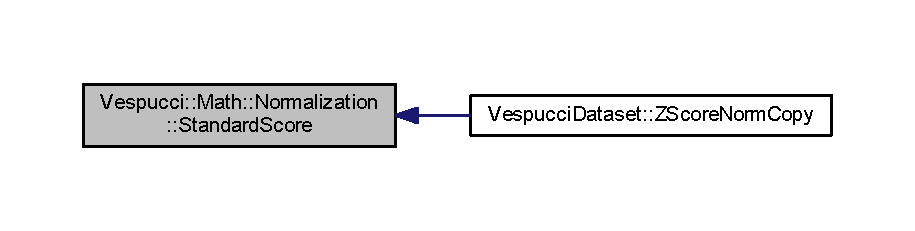
\includegraphics[width=350pt]{namespace_vespucci_1_1_math_1_1_normalization_a8a39e3540561860b69ec95d8d33bfac0_icgraph}
\end{center}
\end{figure}


\hypertarget{namespace_vespucci_1_1_math_1_1_normalization_a00d08eef3567d3420e40dda235c38590}{\index{Vespucci\+::\+Math\+::\+Normalization@{Vespucci\+::\+Math\+::\+Normalization}!Standard\+Score\+Mat@{Standard\+Score\+Mat}}
\index{Standard\+Score\+Mat@{Standard\+Score\+Mat}!Vespucci\+::\+Math\+::\+Normalization@{Vespucci\+::\+Math\+::\+Normalization}}
\subsubsection[{Standard\+Score\+Mat}]{\setlength{\rightskip}{0pt plus 5cm}arma\+::mat Vespucci\+::\+Math\+::\+Normalization\+::\+Standard\+Score\+Mat (
\begin{DoxyParamCaption}
\item[{const arma\+::mat \&}]{X}
\end{DoxyParamCaption}
)}}\label{namespace_vespucci_1_1_math_1_1_normalization_a00d08eef3567d3420e40dda235c38590}


\hyperlink{namespace_vespucci_1_1_math_1_1_normalization_a8a39e3540561860b69ec95d8d33bfac0}{Vespucci\+::\+Math\+::\+Normalization\+::\+Standard\+Score}. 


\begin{DoxyParams}{Parameters}
{\em X} & \\
\hline
\end{DoxyParams}
\begin{DoxyReturn}{Returns}
A arma\+::matrix in which each column of X is replaced by its standard score. 
\end{DoxyReturn}


Definition at line 45 of file normalization.\+cpp.



Here is the caller graph for this function\+:
\nopagebreak
\begin{figure}[H]
\begin{center}
\leavevmode
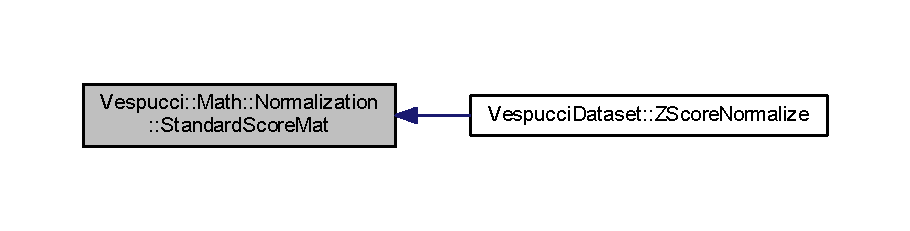
\includegraphics[width=350pt]{namespace_vespucci_1_1_math_1_1_normalization_a00d08eef3567d3420e40dda235c38590_icgraph}
\end{center}
\end{figure}



\hypertarget{namespace_vespucci_1_1_math_1_1_peak_finding}{\section{Vespucci\+:\+:Math\+:\+:Peak\+Finding Namespace Reference}
\label{namespace_vespucci_1_1_math_1_1_peak_finding}\index{Vespucci\+::\+Math\+::\+Peak\+Finding@{Vespucci\+::\+Math\+::\+Peak\+Finding}}
}


A namespace for math functions relating to peak detection and counting.  


\subsection*{Functions}
\begin{DoxyCompactItemize}
\item 
std\+::vector\\*
$<$ \hyperlink{class_vespucci_1_1_math_1_1_c_w_t_ridge}{Vespucci\+::\+Math\+::\+C\+W\+T\+Ridge} $>$ \hyperlink{namespace_vespucci_1_1_math_1_1_peak_finding_aede120546d4e46e4073058508fdd7ae9}{Find\+Ridges} (arma\+::mat \&coefs, arma\+::uvec scales, arma\+::uword gap\+\_\+threshold, arma\+::uword ridge\+\_\+length, arma\+::uword search\+\_\+width, double noise\+\_\+threshold, std\+::string noise\+\_\+method, arma\+::uword noise\+\_\+window)
\begin{DoxyCompactList}\small\item\em \hyperlink{namespace_vespucci_1_1_math_1_1_peak_finding_aede120546d4e46e4073058508fdd7ae9}{Vespucci\+::\+Math\+::\+Peak\+Finding\+::\+Find\+Ridges}. \end{DoxyCompactList}\item 
\hypertarget{namespace_vespucci_1_1_math_1_1_peak_finding_a436ae6b6b68db30f0502e852999077cc}{std\+::vector\\*
$<$ \hyperlink{class_vespucci_1_1_math_1_1_c_w_t_ridge}{Vespucci\+::\+Math\+::\+C\+W\+T\+Ridge} $>$ {\bfseries Link\+Ridges} (const arma\+::sp\+\_\+mat \&maxima, arma\+::uvec scales, arma\+::mat \&coefs, arma\+::uword min\+\_\+window\+\_\+size, arma\+::uword gap\+\_\+threshold)}\label{namespace_vespucci_1_1_math_1_1_peak_finding_a436ae6b6b68db30f0502e852999077cc}

\item 
\hypertarget{namespace_vespucci_1_1_math_1_1_peak_finding_acbebf6b4e4354d20a048d52eb54e6db4}{void {\bfseries Estimate\+Width} (const arma\+::vec \&spectrum, const arma\+::vec \&abscissa, std\+::vector$<$ \hyperlink{class_vespucci_1_1_math_1_1_c_w_t_ridge}{Vespucci\+::\+Math\+::\+C\+W\+T\+Ridge} $>$ \&ridges)}\label{namespace_vespucci_1_1_math_1_1_peak_finding_acbebf6b4e4354d20a048d52eb54e6db4}

\item 
arma\+::vec \hyperlink{namespace_vespucci_1_1_math_1_1_peak_finding_a3d5687d6ba8babb49689af636f28aae8}{Find\+Peaks} (arma\+::vec X, arma\+::vec d\+X, double sel, double threshold, arma\+::vec \&peak\+\_\+magnitudes)
\begin{DoxyCompactList}\small\item\em \hyperlink{namespace_vespucci_1_1_math_1_1_peak_finding_a3d5687d6ba8babb49689af636f28aae8}{Vespucci\+::\+Math\+::\+Peak\+Finding\+::\+Find\+Peaks} an implementation of the peakfinder arma\+::mat\+L\+A\+B routine. \end{DoxyCompactList}\item 
\hypertarget{namespace_vespucci_1_1_math_1_1_peak_finding_a21149205db5d756da8bf91bbc7b71298}{arma\+::uvec {\bfseries Find\+Peak\+Positions} (arma\+::vec X, arma\+::vec d\+X, double sel, double threshold, arma\+::uvec \&local\+\_\+minima)}\label{namespace_vespucci_1_1_math_1_1_peak_finding_a21149205db5d756da8bf91bbc7b71298}

\item 
arma\+::mat \hyperlink{namespace_vespucci_1_1_math_1_1_peak_finding_a9f22a184fb69fb6ab32757fdd19e1ae7}{Find\+Peaks\+Mat} (arma\+::mat X, double sel, double threshold, arma\+::uword poly\+\_\+order, arma\+::uword window\+\_\+size, arma\+::mat \&peak\+\_\+magnitudes)
\begin{DoxyCompactList}\small\item\em \hyperlink{namespace_vespucci_1_1_math_1_1_peak_finding_a9f22a184fb69fb6ab32757fdd19e1ae7}{Vespucci\+::\+Math\+::\+Peak\+Finding\+::\+Find\+Peaks\+Mat} Performs Find\+Peaks on a spectra arma\+::matrix. \end{DoxyCompactList}\item 
arma\+::vec \hyperlink{namespace_vespucci_1_1_math_1_1_peak_finding_a33b834ac6082132d53ec8b307f16e1bd}{Estimate\+Baseline} (arma\+::vec X, arma\+::umat peaks, arma\+::uword window\+\_\+size)
\begin{DoxyCompactList}\small\item\em Estimate\+Baseline. \end{DoxyCompactList}\item 
arma\+::umat \hyperlink{namespace_vespucci_1_1_math_1_1_peak_finding_a502c529617f35fd20d1e11aca2a03a28}{Find\+Peak\+Positions} (arma\+::vec X, arma\+::vec d\+X, double threshold, std\+::string threshold\+\_\+method, arma\+::vec \&peak\+\_\+magnitudes)
\begin{DoxyCompactList}\small\item\em Vespucci\+::\+Math\+::\+Peak\+Finding\+::\+Find\+Peak\+Positions. \end{DoxyCompactList}\item 
\hypertarget{namespace_vespucci_1_1_math_1_1_peak_finding_ab4743c0a36c5000975f1c9f300e101e0}{arma\+::vec {\bfseries Peak\+Population} (arma\+::uword vector\+\_\+size, arma\+::umat peak\+\_\+positions)}\label{namespace_vespucci_1_1_math_1_1_peak_finding_ab4743c0a36c5000975f1c9f300e101e0}

\item 
\hypertarget{namespace_vespucci_1_1_math_1_1_peak_finding_a2106329f1df30b0aca62ccb130494c88}{arma\+::vec {\bfseries Peak\+Extrema} (arma\+::uword vector\+\_\+size, arma\+::umat peak\+\_\+positions)}\label{namespace_vespucci_1_1_math_1_1_peak_finding_a2106329f1df30b0aca62ccb130494c88}

\item 
\hypertarget{namespace_vespucci_1_1_math_1_1_peak_finding_a8a56011b11ff2b0778c7209eeca6a897}{arma\+::mat {\bfseries C\+W\+T\+Peak\+Analysis} (arma\+::mat X, std\+::string wavelet, arma\+::uvec scales, double threshold, std\+::string threshold\+\_\+method, arma\+::mat \&transform)}\label{namespace_vespucci_1_1_math_1_1_peak_finding_a8a56011b11ff2b0778c7209eeca6a897}

\end{DoxyCompactItemize}


\subsection{Detailed Description}
A namespace for math functions relating to peak detection and counting. 

\subsection{Function Documentation}
\hypertarget{namespace_vespucci_1_1_math_1_1_peak_finding_a33b834ac6082132d53ec8b307f16e1bd}{\index{Vespucci\+::\+Math\+::\+Peak\+Finding@{Vespucci\+::\+Math\+::\+Peak\+Finding}!Estimate\+Baseline@{Estimate\+Baseline}}
\index{Estimate\+Baseline@{Estimate\+Baseline}!Vespucci\+::\+Math\+::\+Peak\+Finding@{Vespucci\+::\+Math\+::\+Peak\+Finding}}
\subsubsection[{Estimate\+Baseline}]{\setlength{\rightskip}{0pt plus 5cm}arma\+::vec Vespucci\+::\+Math\+::\+Peak\+Finding\+::\+Estimate\+Baseline (
\begin{DoxyParamCaption}
\item[{arma\+::vec}]{X, }
\item[{arma\+::umat}]{peaks, }
\item[{arma\+::uword}]{window\+\_\+size}
\end{DoxyParamCaption}
)}}\label{namespace_vespucci_1_1_math_1_1_peak_finding_a33b834ac6082132d53ec8b307f16e1bd}


Estimate\+Baseline. 


\begin{DoxyParams}{Parameters}
{\em X} & Signal \\
\hline
{\em peaks} & Positions of peaks to exclude from spectrum to calculate baseline \\
\hline
{\em window\+\_\+size} & Size of local minimum filter applied to baseline \\
\hline
\end{DoxyParams}
\begin{DoxyReturn}{Returns}

\end{DoxyReturn}


Definition at line 352 of file peakfinding.\+cpp.

\hypertarget{namespace_vespucci_1_1_math_1_1_peak_finding_a502c529617f35fd20d1e11aca2a03a28}{\index{Vespucci\+::\+Math\+::\+Peak\+Finding@{Vespucci\+::\+Math\+::\+Peak\+Finding}!Find\+Peak\+Positions@{Find\+Peak\+Positions}}
\index{Find\+Peak\+Positions@{Find\+Peak\+Positions}!Vespucci\+::\+Math\+::\+Peak\+Finding@{Vespucci\+::\+Math\+::\+Peak\+Finding}}
\subsubsection[{Find\+Peak\+Positions}]{\setlength{\rightskip}{0pt plus 5cm}arma\+::umat Vespucci\+::\+Math\+::\+Peak\+Finding\+::\+Find\+Peak\+Positions (
\begin{DoxyParamCaption}
\item[{arma\+::vec}]{X, }
\item[{arma\+::vec}]{d\+X, }
\item[{double}]{threshold, }
\item[{std\+::string}]{threshold\+\_\+method, }
\item[{arma\+::vec \&}]{peak\+\_\+magnitudes}
\end{DoxyParamCaption}
)}}\label{namespace_vespucci_1_1_math_1_1_peak_finding_a502c529617f35fd20d1e11aca2a03a28}


Vespucci\+::\+Math\+::\+Peak\+Finding\+::\+Find\+Peak\+Positions. 


\begin{DoxyParams}{Parameters}
{\em X} & \\
\hline
{\em d\+X} & A buffered first derivative (same size of X with value of X(i) equal to the derivative of X at i. Taken as a parameter incase a smoothed derivative is to be used \\
\hline
{\em threshold} & A value for threshold of significance. Depending on type \\
\hline
{\em threshold\+\_\+method} & Describes the method to be used (see below) \\
\hline
\end{DoxyParams}
\begin{DoxyReturn}{Returns}
A arma\+::umat in which each row represents a peak. The first column contains indices of peak centers, the second column contains the left bound of the peak and the third column contains the right bound of the peak. A arma\+::matrix of this forarma\+::mat is the expected input for \hyperlink{namespace_vespucci_1_1_math_1_1_peak_finding_a33b834ac6082132d53ec8b307f16e1bd}{Vespucci\+::\+Math\+::\+Peak\+Finding\+::\+Estimate\+Baseline}. The peak determination may be carried out on a transformed spectra (such as heavy S-\/\+G smoothing, kernel convolution or C\+W\+T) then Estimate\+Baseline called with these peak centers and the original spectrum. Estimate\+Baseline will then exclude the larger peaks from the baseline. Since Estimate\+Baseline uses a local minimum filter, smaller peaks will be retained while preventing wider peaks from being cut into by the filter.
\end{DoxyReturn}
threshold\+\_\+method can be the following\+: \char`\"{}magnitude\char`\"{} -\/ a minimum peak-\/height threshold, arbitrary double \char`\"{}count\char`\"{} -\/ maximum number of peaks found, largest magnitude first (1 to many) \char`\"{}countpercentage\char`\"{} -\/ largest percentage of all peaks found (0 to 1) \char`\"{}ratio\char`\"{} -\/ ratio of largest magnitude (0 to 1) 

Definition at line 202 of file peakfinding.\+cpp.



Here is the call graph for this function\+:
\nopagebreak
\begin{figure}[H]
\begin{center}
\leavevmode
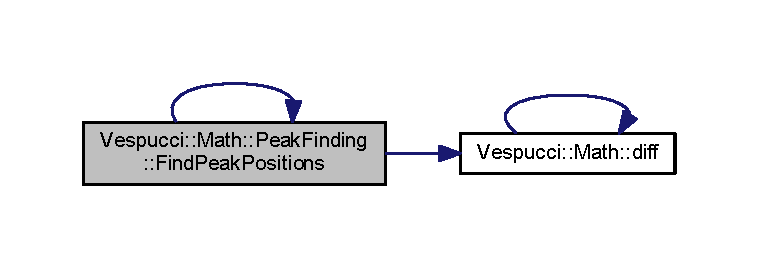
\includegraphics[width=350pt]{namespace_vespucci_1_1_math_1_1_peak_finding_a502c529617f35fd20d1e11aca2a03a28_cgraph}
\end{center}
\end{figure}




Here is the caller graph for this function\+:
\nopagebreak
\begin{figure}[H]
\begin{center}
\leavevmode
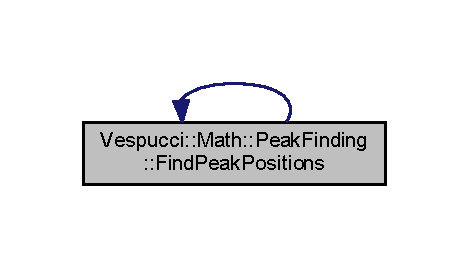
\includegraphics[width=225pt]{namespace_vespucci_1_1_math_1_1_peak_finding_a502c529617f35fd20d1e11aca2a03a28_icgraph}
\end{center}
\end{figure}


\hypertarget{namespace_vespucci_1_1_math_1_1_peak_finding_a3d5687d6ba8babb49689af636f28aae8}{\index{Vespucci\+::\+Math\+::\+Peak\+Finding@{Vespucci\+::\+Math\+::\+Peak\+Finding}!Find\+Peaks@{Find\+Peaks}}
\index{Find\+Peaks@{Find\+Peaks}!Vespucci\+::\+Math\+::\+Peak\+Finding@{Vespucci\+::\+Math\+::\+Peak\+Finding}}
\subsubsection[{Find\+Peaks}]{\setlength{\rightskip}{0pt plus 5cm}arma\+::vec Vespucci\+::\+Math\+::\+Peak\+Finding\+::\+Find\+Peaks (
\begin{DoxyParamCaption}
\item[{arma\+::vec}]{X, }
\item[{arma\+::vec}]{d\+X, }
\item[{double}]{sel, }
\item[{double}]{threshold, }
\item[{arma\+::vec \&}]{peak\+\_\+magnitudes}
\end{DoxyParamCaption}
)}}\label{namespace_vespucci_1_1_math_1_1_peak_finding_a3d5687d6ba8babb49689af636f28aae8}


\hyperlink{namespace_vespucci_1_1_math_1_1_peak_finding_a3d5687d6ba8babb49689af636f28aae8}{Vespucci\+::\+Math\+::\+Peak\+Finding\+::\+Find\+Peaks} an implementation of the peakfinder arma\+::mat\+L\+A\+B routine. 


\begin{DoxyParams}{Parameters}
{\em X} & A vector representing a spectrum \\
\hline
{\em d\+X} & A first-\/derivative spectrum of X \\
\hline
{\em sel} & The amount above surrounding data for a peak to be identified \\
\hline
{\em threshold} & A threshold value which peaks must be larger than to be maxima \\
\hline
{\em poly\+\_\+order} & The polynomial order of the Savitzky-\/\+Golay filter used for derivatization \\
\hline
{\em window\+\_\+size} & The window size of the Savitzky-\/\+Golay filter used for derivatization \\
\hline
{\em peak\+\_\+locations} & A vector containing one and arma\+::zeros corresponding to whether or not a peak center exists at that wavelength \\
\hline
{\em peak\+\_\+magnitudes} & A vector containing values at peak centers. \\
\hline
\end{DoxyParams}
\begin{DoxyReturn}{Returns}

\end{DoxyReturn}


Definition at line 45 of file peakfinding.\+cpp.



Here is the caller graph for this function\+:
\nopagebreak
\begin{figure}[H]
\begin{center}
\leavevmode
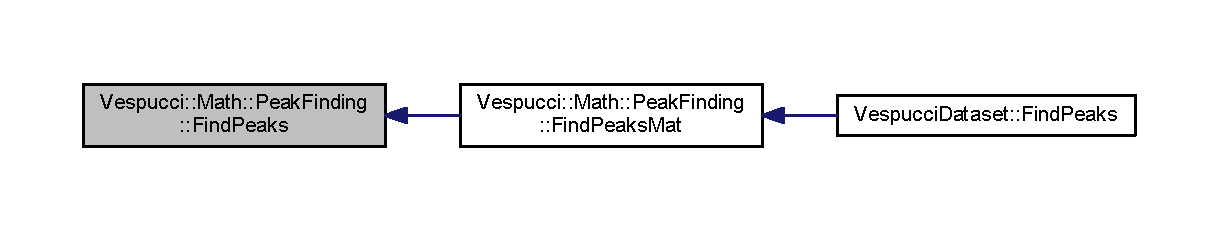
\includegraphics[width=350pt]{namespace_vespucci_1_1_math_1_1_peak_finding_a3d5687d6ba8babb49689af636f28aae8_icgraph}
\end{center}
\end{figure}


\hypertarget{namespace_vespucci_1_1_math_1_1_peak_finding_a9f22a184fb69fb6ab32757fdd19e1ae7}{\index{Vespucci\+::\+Math\+::\+Peak\+Finding@{Vespucci\+::\+Math\+::\+Peak\+Finding}!Find\+Peaks\+Mat@{Find\+Peaks\+Mat}}
\index{Find\+Peaks\+Mat@{Find\+Peaks\+Mat}!Vespucci\+::\+Math\+::\+Peak\+Finding@{Vespucci\+::\+Math\+::\+Peak\+Finding}}
\subsubsection[{Find\+Peaks\+Mat}]{\setlength{\rightskip}{0pt plus 5cm}arma\+::mat Vespucci\+::\+Math\+::\+Peak\+Finding\+::\+Find\+Peaks\+Mat (
\begin{DoxyParamCaption}
\item[{arma\+::mat}]{X, }
\item[{double}]{sel, }
\item[{double}]{threshold, }
\item[{arma\+::uword}]{poly\+\_\+order, }
\item[{arma\+::uword}]{window\+\_\+size, }
\item[{arma\+::mat \&}]{peak\+\_\+magnitudes}
\end{DoxyParamCaption}
)}}\label{namespace_vespucci_1_1_math_1_1_peak_finding_a9f22a184fb69fb6ab32757fdd19e1ae7}


\hyperlink{namespace_vespucci_1_1_math_1_1_peak_finding_a9f22a184fb69fb6ab32757fdd19e1ae7}{Vespucci\+::\+Math\+::\+Peak\+Finding\+::\+Find\+Peaks\+Mat} Performs Find\+Peaks on a spectra arma\+::matrix. 


\begin{DoxyParams}{Parameters}
{\em x} & \\
\hline
{\em sel} & \\
\hline
{\em threshold} & \\
\hline
{\em poly\+\_\+order} & \\
\hline
{\em window\+\_\+size} & \\
\hline
{\em peak\+\_\+locations} & \\
\hline
{\em peak\+\_\+magnitudes} & \\
\hline
\end{DoxyParams}
\begin{DoxyReturn}{Returns}

\end{DoxyReturn}


Definition at line 132 of file peakfinding.\+cpp.



Here is the call graph for this function\+:
\nopagebreak
\begin{figure}[H]
\begin{center}
\leavevmode
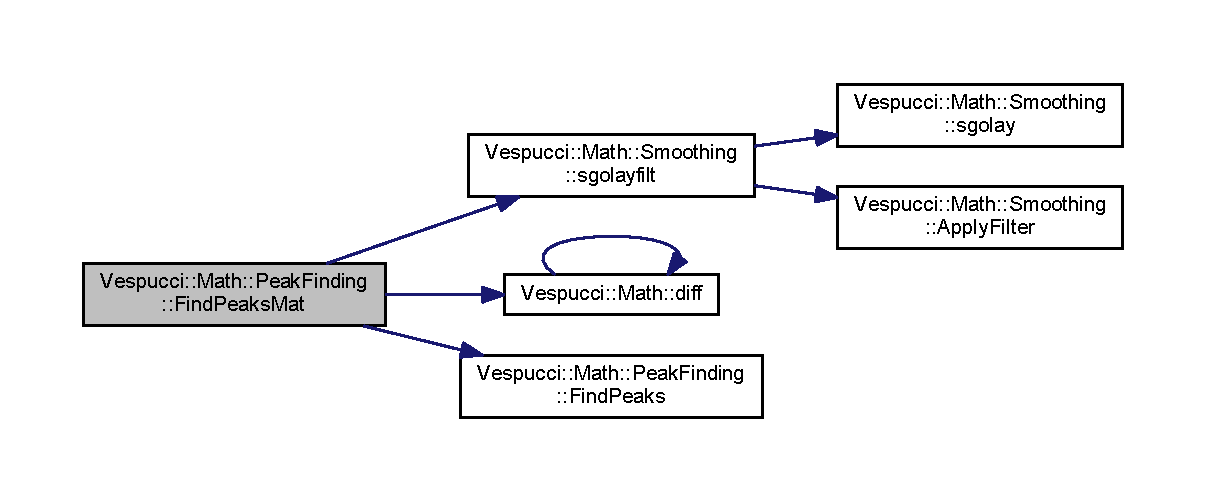
\includegraphics[width=350pt]{namespace_vespucci_1_1_math_1_1_peak_finding_a9f22a184fb69fb6ab32757fdd19e1ae7_cgraph}
\end{center}
\end{figure}




Here is the caller graph for this function\+:
\nopagebreak
\begin{figure}[H]
\begin{center}
\leavevmode
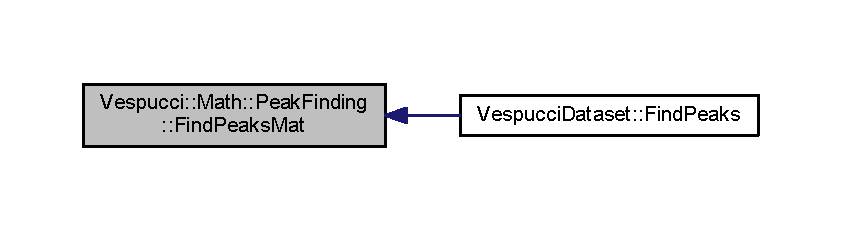
\includegraphics[width=350pt]{namespace_vespucci_1_1_math_1_1_peak_finding_a9f22a184fb69fb6ab32757fdd19e1ae7_icgraph}
\end{center}
\end{figure}


\hypertarget{namespace_vespucci_1_1_math_1_1_peak_finding_aede120546d4e46e4073058508fdd7ae9}{\index{Vespucci\+::\+Math\+::\+Peak\+Finding@{Vespucci\+::\+Math\+::\+Peak\+Finding}!Find\+Ridges@{Find\+Ridges}}
\index{Find\+Ridges@{Find\+Ridges}!Vespucci\+::\+Math\+::\+Peak\+Finding@{Vespucci\+::\+Math\+::\+Peak\+Finding}}
\subsubsection[{Find\+Ridges}]{\setlength{\rightskip}{0pt plus 5cm}std\+::vector$<$ {\bf Vespucci\+::\+Math\+::\+C\+W\+T\+Ridge} $>$ Vespucci\+::\+Math\+::\+Peak\+Finding\+::\+Find\+Ridges (
\begin{DoxyParamCaption}
\item[{arma\+::mat \&}]{coefs, }
\item[{arma\+::uvec}]{scales, }
\item[{arma\+::uword}]{gap\+\_\+threshold, }
\item[{arma\+::uword}]{ridge\+\_\+length, }
\item[{arma\+::uword}]{search\+\_\+width, }
\item[{double}]{noise\+\_\+threshold, }
\item[{std\+::string}]{noise\+\_\+method, }
\item[{arma\+::uword}]{noise\+\_\+window}
\end{DoxyParamCaption}
)}}\label{namespace_vespucci_1_1_math_1_1_peak_finding_aede120546d4e46e4073058508fdd7ae9}


\hyperlink{namespace_vespucci_1_1_math_1_1_peak_finding_aede120546d4e46e4073058508fdd7ae9}{Vespucci\+::\+Math\+::\+Peak\+Finding\+::\+Find\+Ridges}. 


\begin{DoxyParams}{Parameters}
{\em coefs} & \\
\hline
{\em gap\+\_\+threshold} & \\
\hline
{\em ridge\+\_\+length} & \\
\hline
{\em search\+\_\+width} & \\
\hline
\end{DoxyParams}
\begin{DoxyReturn}{Returns}
Identify \char`\"{}ridges\char`\"{} in a C\+W\+T transform matrix. 
\end{DoxyReturn}


Definition at line 433 of file peakfinding.\+cpp.



Here is the call graph for this function\+:
\nopagebreak
\begin{figure}[H]
\begin{center}
\leavevmode
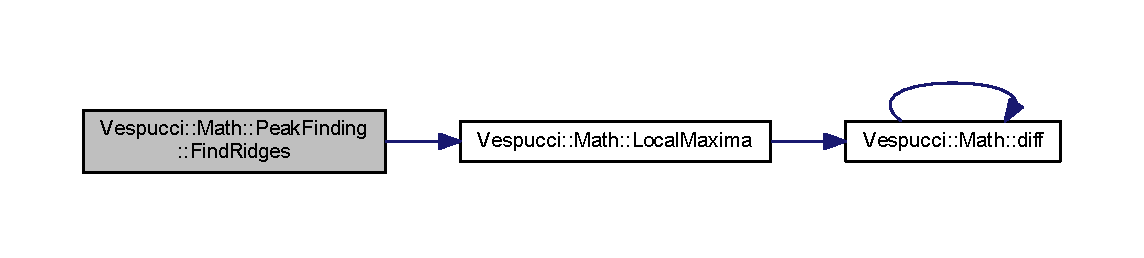
\includegraphics[width=350pt]{namespace_vespucci_1_1_math_1_1_peak_finding_aede120546d4e46e4073058508fdd7ae9_cgraph}
\end{center}
\end{figure}




Here is the caller graph for this function\+:
\nopagebreak
\begin{figure}[H]
\begin{center}
\leavevmode
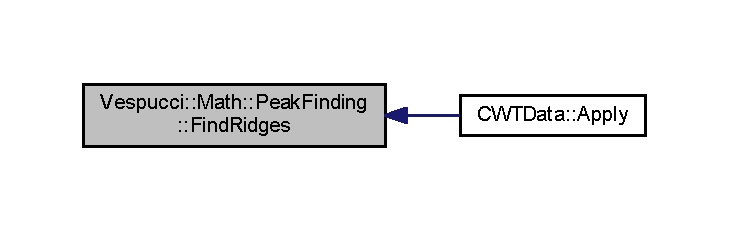
\includegraphics[width=350pt]{namespace_vespucci_1_1_math_1_1_peak_finding_aede120546d4e46e4073058508fdd7ae9_icgraph}
\end{center}
\end{figure}



\hypertarget{namespace_vespucci_1_1_math_1_1_quantification}{\section{Vespucci\+:\+:Math\+:\+:Quantification Namespace Reference}
\label{namespace_vespucci_1_1_math_1_1_quantification}\index{Vespucci\+::\+Math\+::\+Quantification@{Vespucci\+::\+Math\+::\+Quantification}}
}


A namespace for math functions relating to peak quantification.  


\subsection*{Functions}
\begin{DoxyCompactItemize}
\item 
double \hyperlink{namespace_vespucci_1_1_math_1_1_quantification_ad7bdec1b7cc7351cc6c4c5db0c28f069}{Integrate\+Peak} (const arma\+::vec \&X, arma\+::uword min\+\_\+index, arma\+::uword max\+\_\+index, double abscissa\+\_\+step, arma\+::vec \&baseline)
\begin{DoxyCompactList}\small\item\em \hyperlink{namespace_vespucci_1_1_math_1_1_quantification_ad7bdec1b7cc7351cc6c4c5db0c28f069}{Vespucci\+::\+Math\+::\+Quantification\+::\+Integrate\+Peak}. \end{DoxyCompactList}\item 
arma\+::vec \hyperlink{namespace_vespucci_1_1_math_1_1_quantification_a6bc1dd68cd6d9aa6c86d1b57c975f1aa}{Integrate\+Peak\+Mat} (const arma\+::mat \&X, arma\+::vec abscissa, double \&\hyperlink{namespace_vespucci_1_1_math_a884dc00603c6aed8e2ee23988c429c64}{min}, double \&\hyperlink{namespace_vespucci_1_1_math_a3d8f536b4465a4bacce89a51e3854daf}{max}, arma\+::mat \&baselines, arma\+::uvec \&boundaries)
\begin{DoxyCompactList}\small\item\em \hyperlink{namespace_vespucci_1_1_math_1_1_quantification_a6bc1dd68cd6d9aa6c86d1b57c975f1aa}{Vespucci\+::\+Math\+::\+Quantification\+::\+Integrate\+Peak\+Mat}. \end{DoxyCompactList}\item 
arma\+::mat \hyperlink{namespace_vespucci_1_1_math_1_1_quantification_a69e656fff0fae8013961de06b6ff72cc}{Integrate\+Peaks\+Mat} (const arma\+::mat \&X, arma\+::vec abscissa, double \&first\+\_\+min, double \&first\+\_\+max, double \&second\+\_\+min, double \&second\+\_\+max, arma\+::mat \&first\+\_\+baselines, arma\+::mat \&second\+\_\+baselines, arma\+::uvec \&boundaries)
\begin{DoxyCompactList}\small\item\em \hyperlink{namespace_vespucci_1_1_math_1_1_quantification_a69e656fff0fae8013961de06b6ff72cc}{Vespucci\+::\+Math\+::\+Quantification\+::\+Integrate\+Peaks\+Mat}. \end{DoxyCompactList}\item 
double \hyperlink{namespace_vespucci_1_1_math_1_1_quantification_a67d066d37ce165ac3e8c04d97436363c}{Find\+Peak\+Max} (const arma\+::vec \&X, arma\+::uword min\+\_\+index, arma\+::uword max\+\_\+index, arma\+::uword \&\hyperlink{namespace_vespucci_1_1_math_a62f5e835cad1e15513494a5a48e028ae}{position})
\begin{DoxyCompactList}\small\item\em \hyperlink{namespace_vespucci_1_1_math_1_1_quantification_a67d066d37ce165ac3e8c04d97436363c}{Vespucci\+::\+Math\+::\+Quantification\+::\+Find\+Peak\+Max}. \end{DoxyCompactList}\item 
arma\+::vec \hyperlink{namespace_vespucci_1_1_math_1_1_quantification_ac8a29afbde382eddd90a15749a8c3151}{Find\+Peak\+Max\+Mat} (const arma\+::mat \&X, arma\+::vec abscissa, double \&\hyperlink{namespace_vespucci_1_1_math_a884dc00603c6aed8e2ee23988c429c64}{min}, double \&\hyperlink{namespace_vespucci_1_1_math_a3d8f536b4465a4bacce89a51e3854daf}{max}, arma\+::vec \&positions)
\begin{DoxyCompactList}\small\item\em \hyperlink{namespace_vespucci_1_1_math_1_1_quantification_ac8a29afbde382eddd90a15749a8c3151}{Vespucci\+::\+Math\+::\+Quantification\+::\+Find\+Peak\+Max\+Mat}. \end{DoxyCompactList}\item 
arma\+::mat \hyperlink{namespace_vespucci_1_1_math_1_1_quantification_a6b4ad9737e416fb31ffc736465c3e87d}{Find\+Peak\+Maxes\+Mat} (const arma\+::mat \&X, arma\+::vec abscissa, double \&first\+\_\+min, double \&first\+\_\+max, double \&second\+\_\+min, double \&second\+\_\+max, arma\+::mat positions)
\begin{DoxyCompactList}\small\item\em \hyperlink{namespace_vespucci_1_1_math_1_1_quantification_a6b4ad9737e416fb31ffc736465c3e87d}{Vespucci\+::\+Math\+::\+Quantification\+::\+Find\+Peak\+Maxes\+Mat}. \end{DoxyCompactList}\item 
double \hyperlink{namespace_vespucci_1_1_math_1_1_quantification_a9ae95323be0190407aac32ec87605352}{Find\+Bandwidth} (const arma\+::vec \&X, arma\+::uword min\+\_\+index, arma\+::uword max\+\_\+index, arma\+::vec \&midline, arma\+::vec \&baseline, double abscissa\+\_\+step)
\begin{DoxyCompactList}\small\item\em \hyperlink{namespace_vespucci_1_1_math_1_1_quantification_a9ae95323be0190407aac32ec87605352}{Vespucci\+::\+Math\+::\+Quantification\+::\+Find\+Bandwidth}. \end{DoxyCompactList}\item 
arma\+::vec \hyperlink{namespace_vespucci_1_1_math_1_1_quantification_a1f48a5ba0518572ef75a81985a267265}{Find\+Bandwidth\+Mat} (const arma\+::mat \&X, arma\+::vec abscissa, double \&\hyperlink{namespace_vespucci_1_1_math_a884dc00603c6aed8e2ee23988c429c64}{min}, double \&\hyperlink{namespace_vespucci_1_1_math_a3d8f536b4465a4bacce89a51e3854daf}{max}, arma\+::mat \&midlines, arma\+::mat \&baselines, arma\+::uvec \&boundaries)
\begin{DoxyCompactList}\small\item\em \hyperlink{namespace_vespucci_1_1_math_1_1_quantification_a1f48a5ba0518572ef75a81985a267265}{Vespucci\+::\+Math\+::\+Quantification\+::\+Find\+Bandwidth\+Mat}. \end{DoxyCompactList}\item 
\hypertarget{namespace_vespucci_1_1_math_1_1_quantification_a47990289613d7074bbd7d769b5647ff4}{arma\+::vec {\bfseries Correlation\+Mat} (const arma\+::mat \&X, arma\+::vec control)}\label{namespace_vespucci_1_1_math_1_1_quantification_a47990289613d7074bbd7d769b5647ff4}

\end{DoxyCompactItemize}


\subsection{Detailed Description}
A namespace for math functions relating to peak quantification. 

\subsection{Function Documentation}
\hypertarget{namespace_vespucci_1_1_math_1_1_quantification_a9ae95323be0190407aac32ec87605352}{\index{Vespucci\+::\+Math\+::\+Quantification@{Vespucci\+::\+Math\+::\+Quantification}!Find\+Bandwidth@{Find\+Bandwidth}}
\index{Find\+Bandwidth@{Find\+Bandwidth}!Vespucci\+::\+Math\+::\+Quantification@{Vespucci\+::\+Math\+::\+Quantification}}
\subsubsection[{Find\+Bandwidth}]{\setlength{\rightskip}{0pt plus 5cm}double Vespucci\+::\+Math\+::\+Quantification\+::\+Find\+Bandwidth (
\begin{DoxyParamCaption}
\item[{const arma\+::vec \&}]{X, }
\item[{arma\+::uword}]{min\+\_\+index, }
\item[{arma\+::uword}]{max\+\_\+index, }
\item[{arma\+::vec \&}]{midline, }
\item[{arma\+::vec \&}]{baseline, }
\item[{double}]{abscissa\+\_\+step}
\end{DoxyParamCaption}
)}}\label{namespace_vespucci_1_1_math_1_1_quantification_a9ae95323be0190407aac32ec87605352}


\hyperlink{namespace_vespucci_1_1_math_1_1_quantification_a9ae95323be0190407aac32ec87605352}{Vespucci\+::\+Math\+::\+Quantification\+::\+Find\+Bandwidth}. 


\begin{DoxyParams}{Parameters}
{\em X} & \\
\hline
{\em min\+\_\+index} & \\
\hline
{\em max\+\_\+index} & \\
\hline
{\em midline} & \\
\hline
{\em abscissa\+\_\+step} & \\
\hline
\end{DoxyParams}
\begin{DoxyReturn}{Returns}
Finds the full-\/width at half maximum of a peak bound by min\+\_\+index and max\+\_\+index 
\end{DoxyReturn}


Definition at line 32 of file bandwidth.\+cpp.



Here is the caller graph for this function\+:
\nopagebreak
\begin{figure}[H]
\begin{center}
\leavevmode
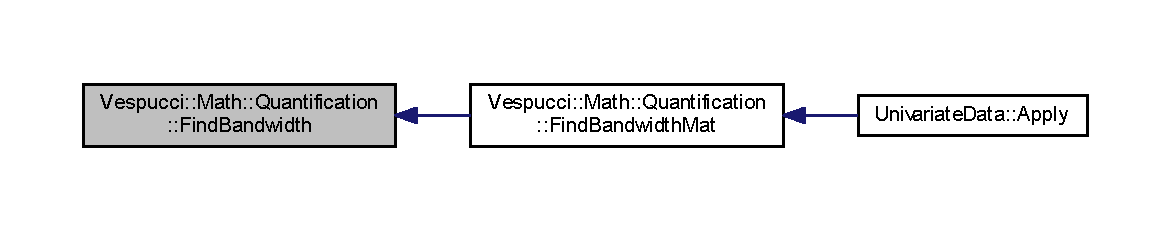
\includegraphics[width=350pt]{namespace_vespucci_1_1_math_1_1_quantification_a9ae95323be0190407aac32ec87605352_icgraph}
\end{center}
\end{figure}


\hypertarget{namespace_vespucci_1_1_math_1_1_quantification_a1f48a5ba0518572ef75a81985a267265}{\index{Vespucci\+::\+Math\+::\+Quantification@{Vespucci\+::\+Math\+::\+Quantification}!Find\+Bandwidth\+Mat@{Find\+Bandwidth\+Mat}}
\index{Find\+Bandwidth\+Mat@{Find\+Bandwidth\+Mat}!Vespucci\+::\+Math\+::\+Quantification@{Vespucci\+::\+Math\+::\+Quantification}}
\subsubsection[{Find\+Bandwidth\+Mat}]{\setlength{\rightskip}{0pt plus 5cm}arma\+::vec Vespucci\+::\+Math\+::\+Quantification\+::\+Find\+Bandwidth\+Mat (
\begin{DoxyParamCaption}
\item[{const arma\+::mat \&}]{X, }
\item[{arma\+::vec}]{abscissa, }
\item[{double \&}]{min, }
\item[{double \&}]{max, }
\item[{arma\+::mat \&}]{midlines, }
\item[{arma\+::mat \&}]{baselines, }
\item[{arma\+::uvec \&}]{boundaries}
\end{DoxyParamCaption}
)}}\label{namespace_vespucci_1_1_math_1_1_quantification_a1f48a5ba0518572ef75a81985a267265}


\hyperlink{namespace_vespucci_1_1_math_1_1_quantification_a1f48a5ba0518572ef75a81985a267265}{Vespucci\+::\+Math\+::\+Quantification\+::\+Find\+Bandwidth\+Mat}. 


\begin{DoxyParams}{Parameters}
{\em X} & \\
\hline
{\em abscissa} & \\
\hline
{\em min} & \\
\hline
{\em max} & \\
\hline
{\em midlines} & \\
\hline
{\em baselines} & \\
\hline
\end{DoxyParams}
\begin{DoxyReturn}{Returns}
Finds the bandwidth of every column of a arma\+::matrix. 
\end{DoxyReturn}


Definition at line 92 of file bandwidth.\+cpp.



Here is the call graph for this function\+:
\nopagebreak
\begin{figure}[H]
\begin{center}
\leavevmode
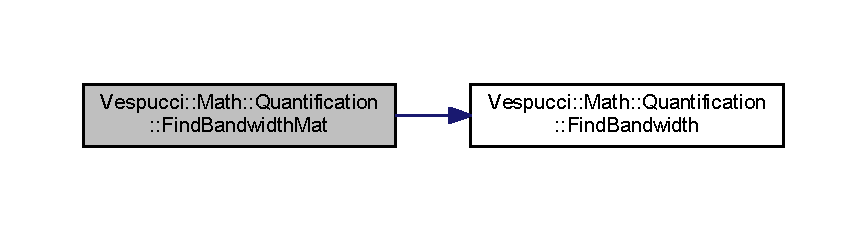
\includegraphics[width=350pt]{namespace_vespucci_1_1_math_1_1_quantification_a1f48a5ba0518572ef75a81985a267265_cgraph}
\end{center}
\end{figure}




Here is the caller graph for this function\+:
\nopagebreak
\begin{figure}[H]
\begin{center}
\leavevmode
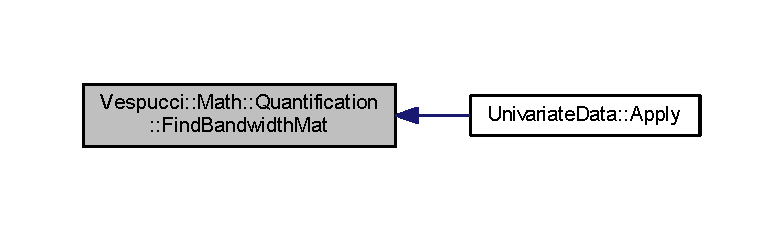
\includegraphics[width=350pt]{namespace_vespucci_1_1_math_1_1_quantification_a1f48a5ba0518572ef75a81985a267265_icgraph}
\end{center}
\end{figure}


\hypertarget{namespace_vespucci_1_1_math_1_1_quantification_a67d066d37ce165ac3e8c04d97436363c}{\index{Vespucci\+::\+Math\+::\+Quantification@{Vespucci\+::\+Math\+::\+Quantification}!Find\+Peak\+Max@{Find\+Peak\+Max}}
\index{Find\+Peak\+Max@{Find\+Peak\+Max}!Vespucci\+::\+Math\+::\+Quantification@{Vespucci\+::\+Math\+::\+Quantification}}
\subsubsection[{Find\+Peak\+Max}]{\setlength{\rightskip}{0pt plus 5cm}double Vespucci\+::\+Math\+::\+Quantification\+::\+Find\+Peak\+Max (
\begin{DoxyParamCaption}
\item[{const arma\+::vec \&}]{X, }
\item[{arma\+::uword}]{min\+\_\+index, }
\item[{arma\+::uword}]{max\+\_\+index, }
\item[{arma\+::uword \&}]{position}
\end{DoxyParamCaption}
)}}\label{namespace_vespucci_1_1_math_1_1_quantification_a67d066d37ce165ac3e8c04d97436363c}


\hyperlink{namespace_vespucci_1_1_math_1_1_quantification_a67d066d37ce165ac3e8c04d97436363c}{Vespucci\+::\+Math\+::\+Quantification\+::\+Find\+Peak\+Max}. 


\begin{DoxyParams}{Parameters}
{\em X} & \\
\hline
{\em min\+\_\+index} & \\
\hline
{\em max\+\_\+index} & \\
\hline
{\em position} & \\
\hline
\end{DoxyParams}
\begin{DoxyReturn}{Returns}
Finds the maximum of a peak bound by min\+\_\+index and max\+\_\+index 
\end{DoxyReturn}


Definition at line 31 of file maximum.\+cpp.



Here is the call graph for this function\+:
\nopagebreak
\begin{figure}[H]
\begin{center}
\leavevmode
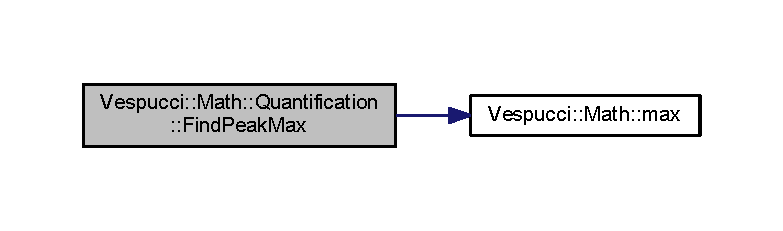
\includegraphics[width=350pt]{namespace_vespucci_1_1_math_1_1_quantification_a67d066d37ce165ac3e8c04d97436363c_cgraph}
\end{center}
\end{figure}




Here is the caller graph for this function\+:
\nopagebreak
\begin{figure}[H]
\begin{center}
\leavevmode
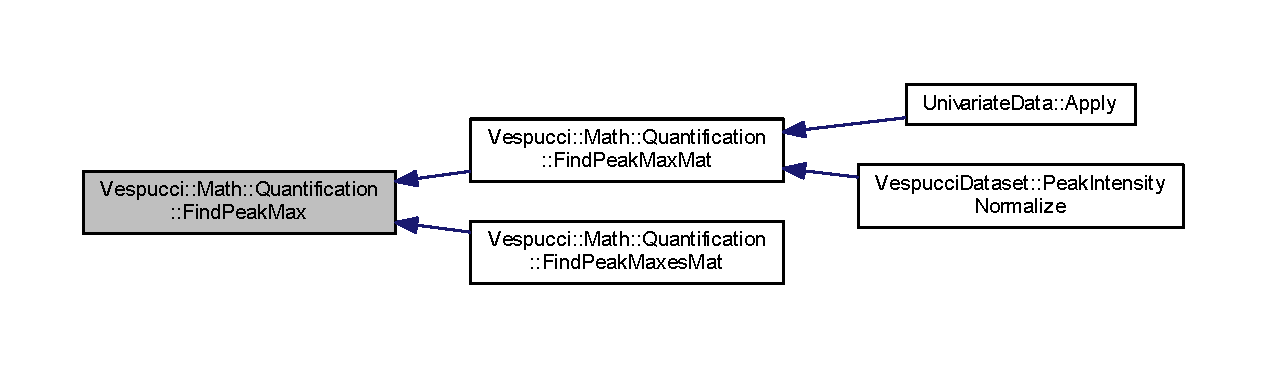
\includegraphics[width=350pt]{namespace_vespucci_1_1_math_1_1_quantification_a67d066d37ce165ac3e8c04d97436363c_icgraph}
\end{center}
\end{figure}


\hypertarget{namespace_vespucci_1_1_math_1_1_quantification_a6b4ad9737e416fb31ffc736465c3e87d}{\index{Vespucci\+::\+Math\+::\+Quantification@{Vespucci\+::\+Math\+::\+Quantification}!Find\+Peak\+Maxes\+Mat@{Find\+Peak\+Maxes\+Mat}}
\index{Find\+Peak\+Maxes\+Mat@{Find\+Peak\+Maxes\+Mat}!Vespucci\+::\+Math\+::\+Quantification@{Vespucci\+::\+Math\+::\+Quantification}}
\subsubsection[{Find\+Peak\+Maxes\+Mat}]{\setlength{\rightskip}{0pt plus 5cm}arma\+::mat Vespucci\+::\+Math\+::\+Quantification\+::\+Find\+Peak\+Maxes\+Mat (
\begin{DoxyParamCaption}
\item[{const arma\+::mat \&}]{X, }
\item[{arma\+::vec}]{abscissa, }
\item[{double \&}]{first\+\_\+min, }
\item[{double \&}]{first\+\_\+max, }
\item[{double \&}]{second\+\_\+min, }
\item[{double \&}]{second\+\_\+max, }
\item[{arma\+::mat}]{positions}
\end{DoxyParamCaption}
)}}\label{namespace_vespucci_1_1_math_1_1_quantification_a6b4ad9737e416fb31ffc736465c3e87d}


\hyperlink{namespace_vespucci_1_1_math_1_1_quantification_a6b4ad9737e416fb31ffc736465c3e87d}{Vespucci\+::\+Math\+::\+Quantification\+::\+Find\+Peak\+Maxes\+Mat}. 


\begin{DoxyParams}{Parameters}
{\em X} & \\
\hline
{\em abscissa} & \\
\hline
{\em first\+\_\+min} & \\
\hline
{\em first\+\_\+max} & \\
\hline
{\em second\+\_\+min} & \\
\hline
{\em second\+\_\+max} & \\
\hline
{\em positions} & \\
\hline
\end{DoxyParams}
\begin{DoxyReturn}{Returns}
Finds two peaks in the manner of Find\+Peak\+Max\+Mat 
\end{DoxyReturn}


Definition at line 84 of file maximum.\+cpp.



Here is the call graph for this function\+:
\nopagebreak
\begin{figure}[H]
\begin{center}
\leavevmode
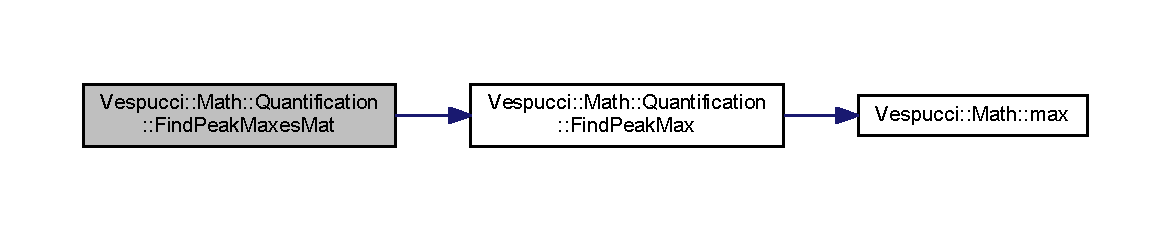
\includegraphics[width=350pt]{namespace_vespucci_1_1_math_1_1_quantification_a6b4ad9737e416fb31ffc736465c3e87d_cgraph}
\end{center}
\end{figure}


\hypertarget{namespace_vespucci_1_1_math_1_1_quantification_ac8a29afbde382eddd90a15749a8c3151}{\index{Vespucci\+::\+Math\+::\+Quantification@{Vespucci\+::\+Math\+::\+Quantification}!Find\+Peak\+Max\+Mat@{Find\+Peak\+Max\+Mat}}
\index{Find\+Peak\+Max\+Mat@{Find\+Peak\+Max\+Mat}!Vespucci\+::\+Math\+::\+Quantification@{Vespucci\+::\+Math\+::\+Quantification}}
\subsubsection[{Find\+Peak\+Max\+Mat}]{\setlength{\rightskip}{0pt plus 5cm}arma\+::vec Vespucci\+::\+Math\+::\+Quantification\+::\+Find\+Peak\+Max\+Mat (
\begin{DoxyParamCaption}
\item[{const arma\+::mat \&}]{X, }
\item[{arma\+::vec}]{abscissa, }
\item[{double \&}]{min, }
\item[{double \&}]{max, }
\item[{arma\+::vec \&}]{positions}
\end{DoxyParamCaption}
)}}\label{namespace_vespucci_1_1_math_1_1_quantification_ac8a29afbde382eddd90a15749a8c3151}


\hyperlink{namespace_vespucci_1_1_math_1_1_quantification_ac8a29afbde382eddd90a15749a8c3151}{Vespucci\+::\+Math\+::\+Quantification\+::\+Find\+Peak\+Max\+Mat}. 


\begin{DoxyParams}{Parameters}
{\em X} & \\
\hline
{\em abscissa} & \\
\hline
{\em min} & \\
\hline
{\em max} & \\
\hline
{\em positions} & \\
\hline
\end{DoxyParams}
\begin{DoxyReturn}{Returns}
Iterates Find\+Peak\+Mat over the columns of a arma\+::matrix. Finds the indices of specified min and max inputs 
\end{DoxyReturn}


Definition at line 50 of file maximum.\+cpp.



Here is the call graph for this function\+:
\nopagebreak
\begin{figure}[H]
\begin{center}
\leavevmode
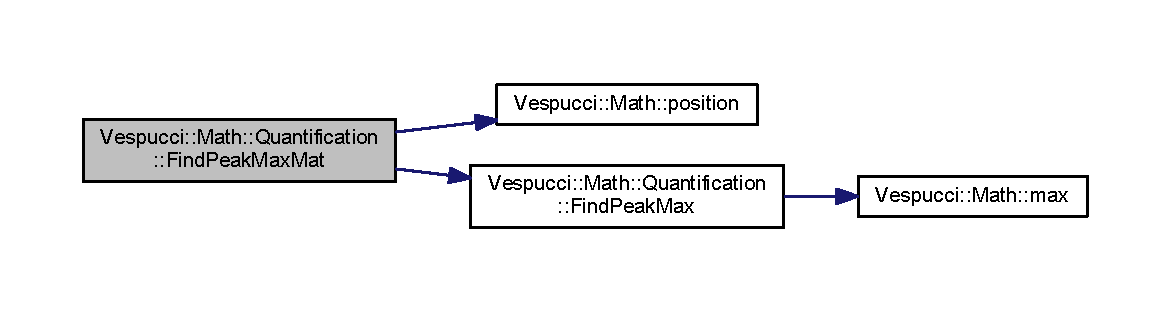
\includegraphics[width=350pt]{namespace_vespucci_1_1_math_1_1_quantification_ac8a29afbde382eddd90a15749a8c3151_cgraph}
\end{center}
\end{figure}




Here is the caller graph for this function\+:
\nopagebreak
\begin{figure}[H]
\begin{center}
\leavevmode
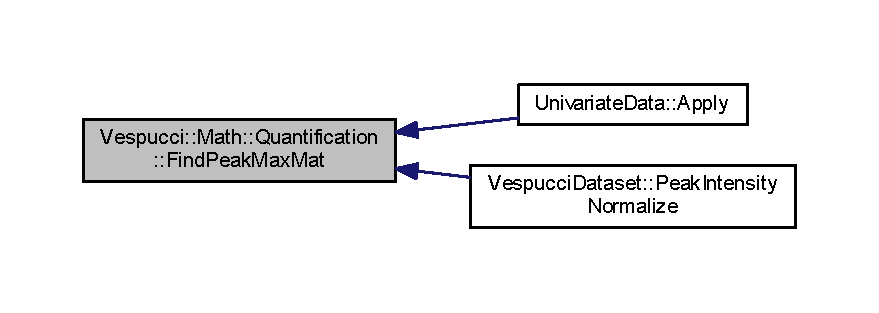
\includegraphics[width=350pt]{namespace_vespucci_1_1_math_1_1_quantification_ac8a29afbde382eddd90a15749a8c3151_icgraph}
\end{center}
\end{figure}


\hypertarget{namespace_vespucci_1_1_math_1_1_quantification_ad7bdec1b7cc7351cc6c4c5db0c28f069}{\index{Vespucci\+::\+Math\+::\+Quantification@{Vespucci\+::\+Math\+::\+Quantification}!Integrate\+Peak@{Integrate\+Peak}}
\index{Integrate\+Peak@{Integrate\+Peak}!Vespucci\+::\+Math\+::\+Quantification@{Vespucci\+::\+Math\+::\+Quantification}}
\subsubsection[{Integrate\+Peak}]{\setlength{\rightskip}{0pt plus 5cm}double Vespucci\+::\+Math\+::\+Quantification\+::\+Integrate\+Peak (
\begin{DoxyParamCaption}
\item[{const arma\+::vec \&}]{X, }
\item[{arma\+::uword}]{min\+\_\+index, }
\item[{arma\+::uword}]{max\+\_\+index, }
\item[{double}]{abscissa\+\_\+step, }
\item[{arma\+::vec \&}]{baseline}
\end{DoxyParamCaption}
)}}\label{namespace_vespucci_1_1_math_1_1_quantification_ad7bdec1b7cc7351cc6c4c5db0c28f069}


\hyperlink{namespace_vespucci_1_1_math_1_1_quantification_ad7bdec1b7cc7351cc6c4c5db0c28f069}{Vespucci\+::\+Math\+::\+Quantification\+::\+Integrate\+Peak}. 


\begin{DoxyParams}{Parameters}
{\em X} & \\
\hline
{\em min\+\_\+index} & \\
\hline
{\em max\+\_\+index} & \\
\hline
{\em abscissa\+\_\+step} & \\
\hline
{\em baseline} & \\
\hline
\end{DoxyParams}
\begin{DoxyReturn}{Returns}
Takes a Riemann sum under a peak defined by certain indices 
\end{DoxyReturn}


Definition at line 31 of file integration.\+cpp.



Here is the caller graph for this function\+:
\nopagebreak
\begin{figure}[H]
\begin{center}
\leavevmode
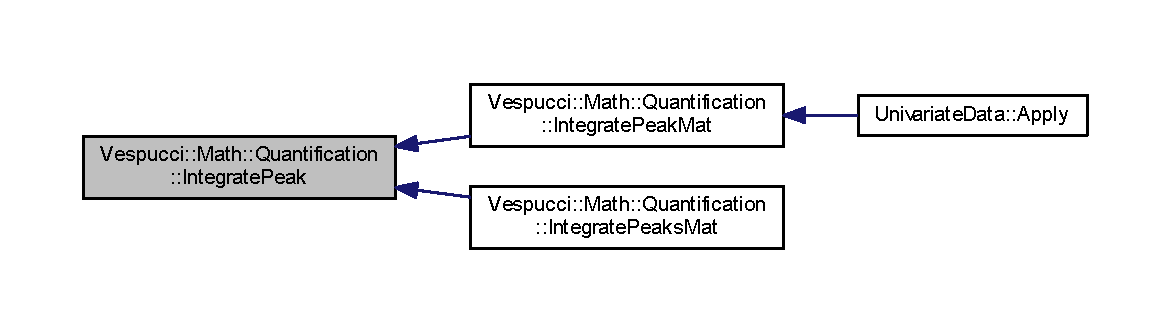
\includegraphics[width=350pt]{namespace_vespucci_1_1_math_1_1_quantification_ad7bdec1b7cc7351cc6c4c5db0c28f069_icgraph}
\end{center}
\end{figure}


\hypertarget{namespace_vespucci_1_1_math_1_1_quantification_a6bc1dd68cd6d9aa6c86d1b57c975f1aa}{\index{Vespucci\+::\+Math\+::\+Quantification@{Vespucci\+::\+Math\+::\+Quantification}!Integrate\+Peak\+Mat@{Integrate\+Peak\+Mat}}
\index{Integrate\+Peak\+Mat@{Integrate\+Peak\+Mat}!Vespucci\+::\+Math\+::\+Quantification@{Vespucci\+::\+Math\+::\+Quantification}}
\subsubsection[{Integrate\+Peak\+Mat}]{\setlength{\rightskip}{0pt plus 5cm}arma\+::vec Vespucci\+::\+Math\+::\+Quantification\+::\+Integrate\+Peak\+Mat (
\begin{DoxyParamCaption}
\item[{const arma\+::mat \&}]{X, }
\item[{arma\+::vec}]{abscissa, }
\item[{double \&}]{min, }
\item[{double \&}]{max, }
\item[{arma\+::mat \&}]{baselines, }
\item[{arma\+::uvec \&}]{boundaries}
\end{DoxyParamCaption}
)}}\label{namespace_vespucci_1_1_math_1_1_quantification_a6bc1dd68cd6d9aa6c86d1b57c975f1aa}


\hyperlink{namespace_vespucci_1_1_math_1_1_quantification_a6bc1dd68cd6d9aa6c86d1b57c975f1aa}{Vespucci\+::\+Math\+::\+Quantification\+::\+Integrate\+Peak\+Mat}. 


\begin{DoxyParams}{Parameters}
{\em X} & \\
\hline
{\em abscissa} & \\
\hline
{\em min} & \\
\hline
{\em max} & \\
\hline
{\em baselines} & \\
\hline
\end{DoxyParams}
\begin{DoxyReturn}{Returns}
Finds the index of specified start and end values, then calls Integrate\+Peak on each column of the arma\+::matrix 
\end{DoxyReturn}


Definition at line 56 of file integration.\+cpp.



Here is the call graph for this function\+:
\nopagebreak
\begin{figure}[H]
\begin{center}
\leavevmode
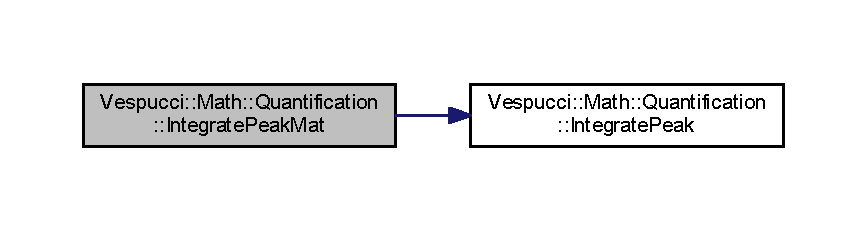
\includegraphics[width=350pt]{namespace_vespucci_1_1_math_1_1_quantification_a6bc1dd68cd6d9aa6c86d1b57c975f1aa_cgraph}
\end{center}
\end{figure}




Here is the caller graph for this function\+:
\nopagebreak
\begin{figure}[H]
\begin{center}
\leavevmode
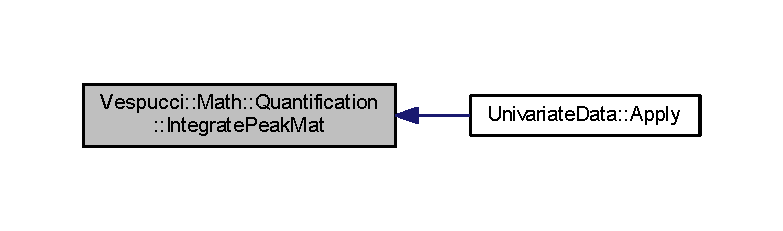
\includegraphics[width=350pt]{namespace_vespucci_1_1_math_1_1_quantification_a6bc1dd68cd6d9aa6c86d1b57c975f1aa_icgraph}
\end{center}
\end{figure}


\hypertarget{namespace_vespucci_1_1_math_1_1_quantification_a69e656fff0fae8013961de06b6ff72cc}{\index{Vespucci\+::\+Math\+::\+Quantification@{Vespucci\+::\+Math\+::\+Quantification}!Integrate\+Peaks\+Mat@{Integrate\+Peaks\+Mat}}
\index{Integrate\+Peaks\+Mat@{Integrate\+Peaks\+Mat}!Vespucci\+::\+Math\+::\+Quantification@{Vespucci\+::\+Math\+::\+Quantification}}
\subsubsection[{Integrate\+Peaks\+Mat}]{\setlength{\rightskip}{0pt plus 5cm}arma\+::mat Vespucci\+::\+Math\+::\+Quantification\+::\+Integrate\+Peaks\+Mat (
\begin{DoxyParamCaption}
\item[{const arma\+::mat \&}]{X, }
\item[{arma\+::vec}]{abscissa, }
\item[{double \&}]{first\+\_\+min, }
\item[{double \&}]{first\+\_\+max, }
\item[{double \&}]{second\+\_\+min, }
\item[{double \&}]{second\+\_\+max, }
\item[{arma\+::mat \&}]{first\+\_\+baselines, }
\item[{arma\+::mat \&}]{second\+\_\+baselines, }
\item[{arma\+::uvec \&}]{boundaries}
\end{DoxyParamCaption}
)}}\label{namespace_vespucci_1_1_math_1_1_quantification_a69e656fff0fae8013961de06b6ff72cc}


\hyperlink{namespace_vespucci_1_1_math_1_1_quantification_a69e656fff0fae8013961de06b6ff72cc}{Vespucci\+::\+Math\+::\+Quantification\+::\+Integrate\+Peaks\+Mat}. 


\begin{DoxyParams}{Parameters}
{\em X} & \\
\hline
{\em abscissa} & \\
\hline
{\em first\+\_\+min} & \\
\hline
{\em first\+\_\+max} & \\
\hline
{\em second\+\_\+min} & \\
\hline
{\em second\+\_\+max} & \\
\hline
{\em first\+\_\+baselines} & \\
\hline
{\em second\+\_\+baselines} & \\
\hline
\end{DoxyParams}
\begin{DoxyReturn}{Returns}
Performs two peak integrations 
\end{DoxyReturn}


Definition at line 90 of file integration.\+cpp.



Here is the call graph for this function\+:
\nopagebreak
\begin{figure}[H]
\begin{center}
\leavevmode
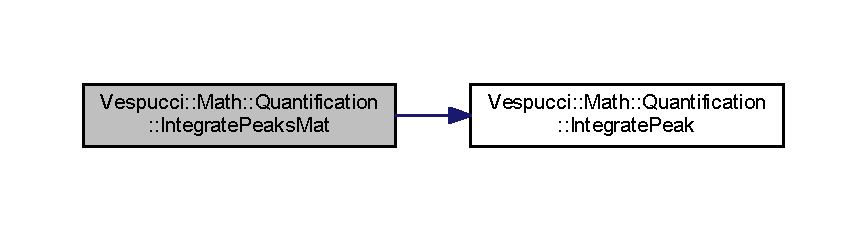
\includegraphics[width=350pt]{namespace_vespucci_1_1_math_1_1_quantification_a69e656fff0fae8013961de06b6ff72cc_cgraph}
\end{center}
\end{figure}



\hypertarget{namespace_vespucci_1_1_math_1_1_smoothing}{\section{Vespucci\+:\+:Math\+:\+:Smoothing Namespace Reference}
\label{namespace_vespucci_1_1_math_1_1_smoothing}\index{Vespucci\+::\+Math\+::\+Smoothing@{Vespucci\+::\+Math\+::\+Smoothing}}
}


A namespace for math functions relating to filtering and smoothing signals.  


\subsection*{Functions}
\begin{DoxyCompactItemize}
\item 
arma\+::mat \hyperlink{namespace_vespucci_1_1_math_1_1_smoothing_a0fb8087861e1d4b8f05dd4dff3cdb012}{sgolay} (arma\+::uword poly\+\_\+order, arma\+::uword window\+\_\+size, arma\+::uword deriv\+\_\+order, arma\+::uword scaling\+\_\+factor)
\begin{DoxyCompactList}\small\item\em \hyperlink{namespace_vespucci_1_1_math_1_1_smoothing_a0fb8087861e1d4b8f05dd4dff3cdb012}{Vespucci\+::\+Math\+::\+Smoothing\+::sgolay} Find a arma\+::matrix of Savitzky-\/\+Golay convolution coefficients. \end{DoxyCompactList}\item 
arma\+::mat \hyperlink{namespace_vespucci_1_1_math_1_1_smoothing_a2cb17f59d170c1ca2437b264d13626b6}{sgolayfilt} (const arma\+::mat \&x, arma\+::uword poly\+\_\+order, arma\+::uword window\+\_\+size, arma\+::uword deriv\+\_\+order, arma\+::uword scaling\+\_\+factor)
\begin{DoxyCompactList}\small\item\em sgolayfilt Apply Savitzky-\/\+Golay smoothing to each column of a arma\+::matrix \end{DoxyCompactList}\item 
arma\+::vec \hyperlink{namespace_vespucci_1_1_math_1_1_smoothing_aa38f2ef278486993ec066ff5701bec62}{Apply\+Filter} (const arma\+::vec \&x, arma\+::mat coefficients, arma\+::uword window\+\_\+size)
\begin{DoxyCompactList}\small\item\em \hyperlink{namespace_vespucci_1_1_math_1_1_smoothing_aa38f2ef278486993ec066ff5701bec62}{Vespucci\+::\+Math\+::\+Smoothing\+::\+Apply\+Filter} Apply F\+I\+R filters to a column vector. \end{DoxyCompactList}\item 
arma\+::vec \hyperlink{namespace_vespucci_1_1_math_1_1_smoothing_ae7edb32bb2b859965dae5626b829e0cf}{Apply\+Filter} (const arma\+::vec \&x, arma\+::vec filter)
\begin{DoxyCompactList}\small\item\em \hyperlink{namespace_vespucci_1_1_math_1_1_smoothing_aa38f2ef278486993ec066ff5701bec62}{Vespucci\+::\+Math\+::\+Smoothing\+::\+Apply\+Filter}. \end{DoxyCompactList}\item 
arma\+::vec \hyperlink{namespace_vespucci_1_1_math_1_1_smoothing_a611221f749d15133ad90da3ba3bbca73}{Create\+Moving\+Average\+Filter} (arma\+::uword window\+\_\+size)
\begin{DoxyCompactList}\small\item\em \hyperlink{namespace_vespucci_1_1_math_1_1_smoothing_a611221f749d15133ad90da3ba3bbca73}{Vespucci\+::\+Math\+::\+Smoothing\+::\+Create\+Moving\+Average\+Filter}. \end{DoxyCompactList}\item 
arma\+::vec \hyperlink{namespace_vespucci_1_1_math_1_1_smoothing_a5456df71022c23baab4c51988866656e}{Median\+Filter} (const arma\+::vec \&X, arma\+::uword window\+\_\+size)
\begin{DoxyCompactList}\small\item\em \hyperlink{namespace_vespucci_1_1_math_1_1_smoothing_a5456df71022c23baab4c51988866656e}{Vespucci\+::\+Math\+::\+Smoothing\+::\+Median\+Filter}. \end{DoxyCompactList}\item 
arma\+::mat \hyperlink{namespace_vespucci_1_1_math_1_1_smoothing_a2b168115738d2931e0a5504823b26b3b}{Median\+Filter\+Mat} (const arma\+::mat \&X, arma\+::uword window\+\_\+size)
\begin{DoxyCompactList}\small\item\em \hyperlink{namespace_vespucci_1_1_math_1_1_smoothing_a2b168115738d2931e0a5504823b26b3b}{Vespucci\+::\+Math\+::\+Smoothing\+::\+Median\+Filter\+Mat}. \end{DoxyCompactList}\item 
arma\+::vec \hyperlink{namespace_vespucci_1_1_math_1_1_smoothing_ab92bb85566a363c2c54ad77d4eb2468f}{Whittaker\+Smooth} (const arma\+::vec \&x, double lambda, arma\+::uword penalty\+\_\+order)
\begin{DoxyCompactList}\small\item\em Vespucci\+::\+Math\+::\+Whittaker\+Smooth. \end{DoxyCompactList}\end{DoxyCompactItemize}


\subsection{Detailed Description}
A namespace for math functions relating to filtering and smoothing signals. 

\subsection{Function Documentation}
\hypertarget{namespace_vespucci_1_1_math_1_1_smoothing_aa38f2ef278486993ec066ff5701bec62}{\index{Vespucci\+::\+Math\+::\+Smoothing@{Vespucci\+::\+Math\+::\+Smoothing}!Apply\+Filter@{Apply\+Filter}}
\index{Apply\+Filter@{Apply\+Filter}!Vespucci\+::\+Math\+::\+Smoothing@{Vespucci\+::\+Math\+::\+Smoothing}}
\subsubsection[{Apply\+Filter}]{\setlength{\rightskip}{0pt plus 5cm}arma\+::vec Vespucci\+::\+Math\+::\+Smoothing\+::\+Apply\+Filter (
\begin{DoxyParamCaption}
\item[{const arma\+::vec \&}]{x, }
\item[{arma\+::mat}]{coefficients, }
\item[{arma\+::uword}]{window\+\_\+size}
\end{DoxyParamCaption}
)}}\label{namespace_vespucci_1_1_math_1_1_smoothing_aa38f2ef278486993ec066ff5701bec62}


\hyperlink{namespace_vespucci_1_1_math_1_1_smoothing_aa38f2ef278486993ec066ff5701bec62}{Vespucci\+::\+Math\+::\+Smoothing\+::\+Apply\+Filter} Apply F\+I\+R filters to a column vector. 


\begin{DoxyParams}{Parameters}
{\em x} & Data to be filtered \\
\hline
{\em coefficients} & A arma\+::matrix of F\+I\+R filters. \\
\hline
{\em window\+\_\+size} & Filter window size \\
\hline
\end{DoxyParams}
\begin{DoxyReturn}{Returns}
Filtered data Apply F\+I\+R filters to a column vector. The central row of coefficients contains the filter used for most of the data. The first (window\+\_\+size -\/ 1)/2 rows are filtered with the lower rows ofccoefficients, and likewise for the last (window\+\_\+size -\/ 1)/2 rows and the first rows of coefficients. 
\end{DoxyReturn}


Definition at line 127 of file F\+I\+R.\+cpp.



Here is the caller graph for this function\+:
\nopagebreak
\begin{figure}[H]
\begin{center}
\leavevmode
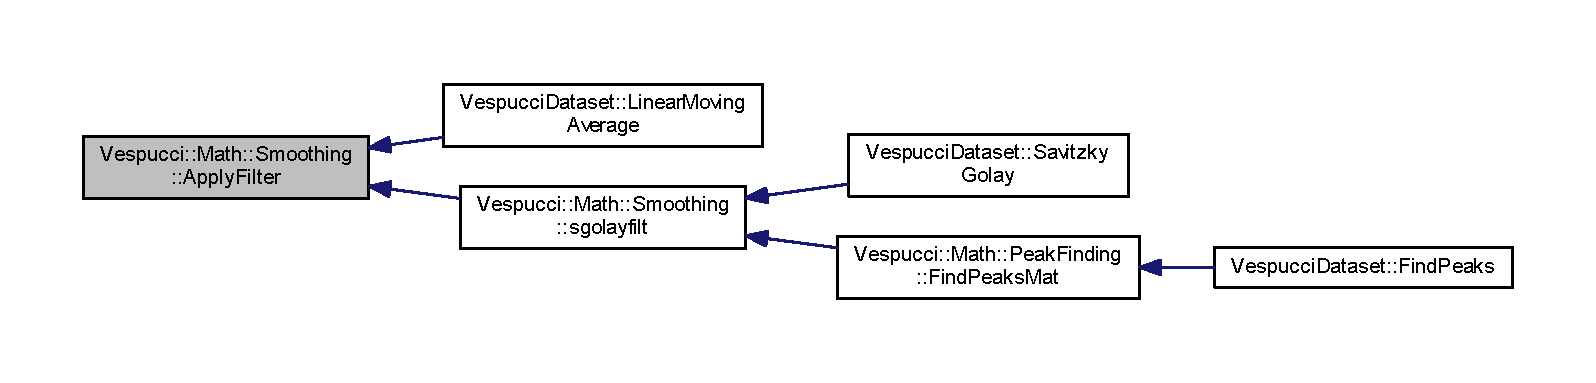
\includegraphics[width=350pt]{namespace_vespucci_1_1_math_1_1_smoothing_aa38f2ef278486993ec066ff5701bec62_icgraph}
\end{center}
\end{figure}


\hypertarget{namespace_vespucci_1_1_math_1_1_smoothing_ae7edb32bb2b859965dae5626b829e0cf}{\index{Vespucci\+::\+Math\+::\+Smoothing@{Vespucci\+::\+Math\+::\+Smoothing}!Apply\+Filter@{Apply\+Filter}}
\index{Apply\+Filter@{Apply\+Filter}!Vespucci\+::\+Math\+::\+Smoothing@{Vespucci\+::\+Math\+::\+Smoothing}}
\subsubsection[{Apply\+Filter}]{\setlength{\rightskip}{0pt plus 5cm}arma\+::vec Vespucci\+::\+Math\+::\+Smoothing\+::\+Apply\+Filter (
\begin{DoxyParamCaption}
\item[{const arma\+::vec \&}]{x, }
\item[{arma\+::vec}]{filter}
\end{DoxyParamCaption}
)}}\label{namespace_vespucci_1_1_math_1_1_smoothing_ae7edb32bb2b859965dae5626b829e0cf}


\hyperlink{namespace_vespucci_1_1_math_1_1_smoothing_aa38f2ef278486993ec066ff5701bec62}{Vespucci\+::\+Math\+::\+Smoothing\+::\+Apply\+Filter}. 


\begin{DoxyParams}{Parameters}
{\em x} & The vector to filter \\
\hline
{\em filter} & The filter \\
\hline
\end{DoxyParams}
\begin{DoxyReturn}{Returns}
Filtered data Applies an F\+I\+R filter to x 
\end{DoxyReturn}


Definition at line 148 of file F\+I\+R.\+cpp.

\hypertarget{namespace_vespucci_1_1_math_1_1_smoothing_a611221f749d15133ad90da3ba3bbca73}{\index{Vespucci\+::\+Math\+::\+Smoothing@{Vespucci\+::\+Math\+::\+Smoothing}!Create\+Moving\+Average\+Filter@{Create\+Moving\+Average\+Filter}}
\index{Create\+Moving\+Average\+Filter@{Create\+Moving\+Average\+Filter}!Vespucci\+::\+Math\+::\+Smoothing@{Vespucci\+::\+Math\+::\+Smoothing}}
\subsubsection[{Create\+Moving\+Average\+Filter}]{\setlength{\rightskip}{0pt plus 5cm}arma\+::vec Vespucci\+::\+Math\+::\+Smoothing\+::\+Create\+Moving\+Average\+Filter (
\begin{DoxyParamCaption}
\item[{arma\+::uword}]{window\+\_\+size}
\end{DoxyParamCaption}
)}}\label{namespace_vespucci_1_1_math_1_1_smoothing_a611221f749d15133ad90da3ba3bbca73}


\hyperlink{namespace_vespucci_1_1_math_1_1_smoothing_a611221f749d15133ad90da3ba3bbca73}{Vespucci\+::\+Math\+::\+Smoothing\+::\+Create\+Moving\+Average\+Filter}. 


\begin{DoxyParams}{Parameters}
{\em window\+\_\+size} & The window size of the filter. \\
\hline
\end{DoxyParams}
\begin{DoxyReturn}{Returns}
A moving average filter Create a moving average filter of a certain window size. 
\end{DoxyReturn}


Definition at line 165 of file F\+I\+R.\+cpp.



Here is the caller graph for this function\+:
\nopagebreak
\begin{figure}[H]
\begin{center}
\leavevmode
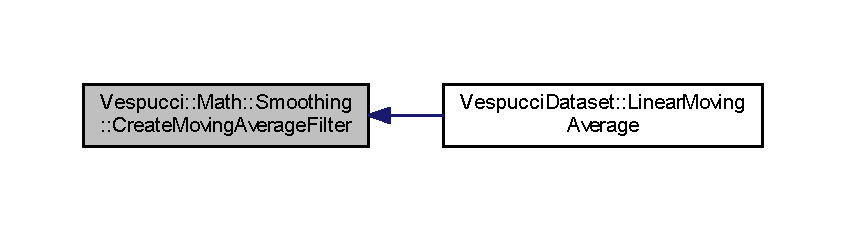
\includegraphics[width=350pt]{namespace_vespucci_1_1_math_1_1_smoothing_a611221f749d15133ad90da3ba3bbca73_icgraph}
\end{center}
\end{figure}


\hypertarget{namespace_vespucci_1_1_math_1_1_smoothing_a5456df71022c23baab4c51988866656e}{\index{Vespucci\+::\+Math\+::\+Smoothing@{Vespucci\+::\+Math\+::\+Smoothing}!Median\+Filter@{Median\+Filter}}
\index{Median\+Filter@{Median\+Filter}!Vespucci\+::\+Math\+::\+Smoothing@{Vespucci\+::\+Math\+::\+Smoothing}}
\subsubsection[{Median\+Filter}]{\setlength{\rightskip}{0pt plus 5cm}arma\+::vec Vespucci\+::\+Math\+::\+Smoothing\+::\+Median\+Filter (
\begin{DoxyParamCaption}
\item[{const arma\+::vec \&}]{X, }
\item[{arma\+::uword}]{window\+\_\+size}
\end{DoxyParamCaption}
)}}\label{namespace_vespucci_1_1_math_1_1_smoothing_a5456df71022c23baab4c51988866656e}


\hyperlink{namespace_vespucci_1_1_math_1_1_smoothing_a5456df71022c23baab4c51988866656e}{Vespucci\+::\+Math\+::\+Smoothing\+::\+Median\+Filter}. 


\begin{DoxyParams}{Parameters}
{\em X} & \\
\hline
{\em window\+\_\+size} & \\
\hline
\end{DoxyParams}
\begin{DoxyReturn}{Returns}
Performs median filtering on a signal X. This just ignores the edges becuause they will be fairly small and not very interesting. 
\end{DoxyReturn}


Definition at line 29 of file nonlinear.\+cpp.



Here is the caller graph for this function\+:
\nopagebreak
\begin{figure}[H]
\begin{center}
\leavevmode
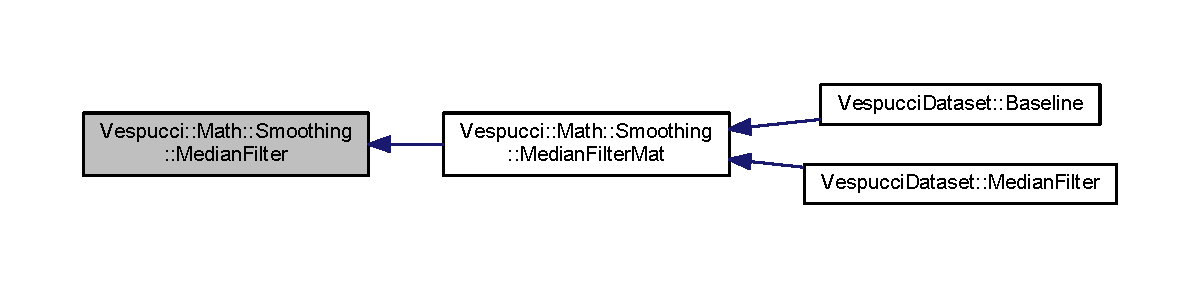
\includegraphics[width=350pt]{namespace_vespucci_1_1_math_1_1_smoothing_a5456df71022c23baab4c51988866656e_icgraph}
\end{center}
\end{figure}


\hypertarget{namespace_vespucci_1_1_math_1_1_smoothing_a2b168115738d2931e0a5504823b26b3b}{\index{Vespucci\+::\+Math\+::\+Smoothing@{Vespucci\+::\+Math\+::\+Smoothing}!Median\+Filter\+Mat@{Median\+Filter\+Mat}}
\index{Median\+Filter\+Mat@{Median\+Filter\+Mat}!Vespucci\+::\+Math\+::\+Smoothing@{Vespucci\+::\+Math\+::\+Smoothing}}
\subsubsection[{Median\+Filter\+Mat}]{\setlength{\rightskip}{0pt plus 5cm}arma\+::mat Vespucci\+::\+Math\+::\+Smoothing\+::\+Median\+Filter\+Mat (
\begin{DoxyParamCaption}
\item[{const arma\+::mat \&}]{X, }
\item[{arma\+::uword}]{window\+\_\+size}
\end{DoxyParamCaption}
)}}\label{namespace_vespucci_1_1_math_1_1_smoothing_a2b168115738d2931e0a5504823b26b3b}


\hyperlink{namespace_vespucci_1_1_math_1_1_smoothing_a2b168115738d2931e0a5504823b26b3b}{Vespucci\+::\+Math\+::\+Smoothing\+::\+Median\+Filter\+Mat}. 


\begin{DoxyParams}{Parameters}
{\em X} & \\
\hline
{\em window\+\_\+size} & \\
\hline
\end{DoxyParams}
\begin{DoxyReturn}{Returns}
Performs Median Filter over a arma\+::matrix with spectra in columns 
\end{DoxyReturn}


Definition at line 60 of file nonlinear.\+cpp.



Here is the call graph for this function\+:
\nopagebreak
\begin{figure}[H]
\begin{center}
\leavevmode
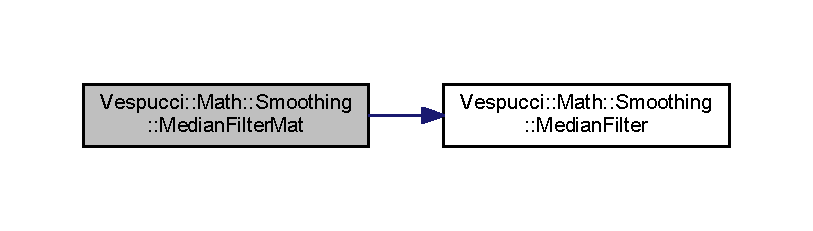
\includegraphics[width=350pt]{namespace_vespucci_1_1_math_1_1_smoothing_a2b168115738d2931e0a5504823b26b3b_cgraph}
\end{center}
\end{figure}




Here is the caller graph for this function\+:
\nopagebreak
\begin{figure}[H]
\begin{center}
\leavevmode
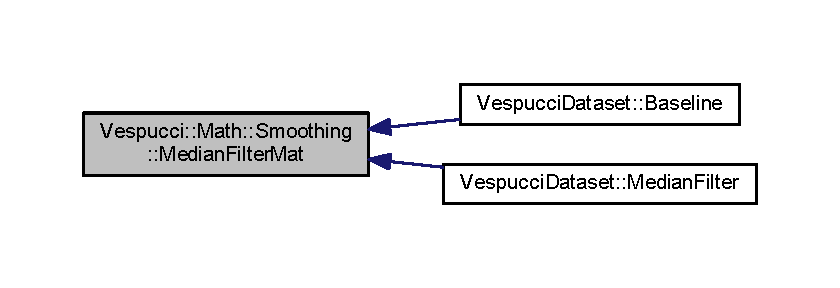
\includegraphics[width=350pt]{namespace_vespucci_1_1_math_1_1_smoothing_a2b168115738d2931e0a5504823b26b3b_icgraph}
\end{center}
\end{figure}


\hypertarget{namespace_vespucci_1_1_math_1_1_smoothing_a0fb8087861e1d4b8f05dd4dff3cdb012}{\index{Vespucci\+::\+Math\+::\+Smoothing@{Vespucci\+::\+Math\+::\+Smoothing}!sgolay@{sgolay}}
\index{sgolay@{sgolay}!Vespucci\+::\+Math\+::\+Smoothing@{Vespucci\+::\+Math\+::\+Smoothing}}
\subsubsection[{sgolay}]{\setlength{\rightskip}{0pt plus 5cm}arma\+::mat Vespucci\+::\+Math\+::\+Smoothing\+::sgolay (
\begin{DoxyParamCaption}
\item[{arma\+::uword}]{poly\+\_\+order, }
\item[{arma\+::uword}]{window\+\_\+size, }
\item[{arma\+::uword}]{deriv\+\_\+order, }
\item[{arma\+::uword}]{scaling\+\_\+factor}
\end{DoxyParamCaption}
)}}\label{namespace_vespucci_1_1_math_1_1_smoothing_a0fb8087861e1d4b8f05dd4dff3cdb012}


\hyperlink{namespace_vespucci_1_1_math_1_1_smoothing_a0fb8087861e1d4b8f05dd4dff3cdb012}{Vespucci\+::\+Math\+::\+Smoothing\+::sgolay} Find a arma\+::matrix of Savitzky-\/\+Golay convolution coefficients. 


\begin{DoxyParams}{Parameters}
{\em poly\+\_\+order} & \\
\hline
{\em window\+\_\+size} & \\
\hline
{\em deriv\+\_\+order} & \\
\hline
{\em scaling\+\_\+factor} & \\
\hline
\end{DoxyParams}
\begin{DoxyReturn}{Returns}
A arma\+::matrix of size window\+\_\+size by window\+\_\+size containing coefficients. Finds a arma\+::matrix of Savitzky-\/\+Golay convolution coefficients, similar to the sgolay function in the Octave and arma\+::mat\+L\+A\+B signal packages. The central row is the filter used for most of the dataset. The outer rows are used on the edges of the signal to be filtered. 
\end{DoxyReturn}


Definition at line 37 of file F\+I\+R.\+cpp.



Here is the caller graph for this function\+:
\nopagebreak
\begin{figure}[H]
\begin{center}
\leavevmode
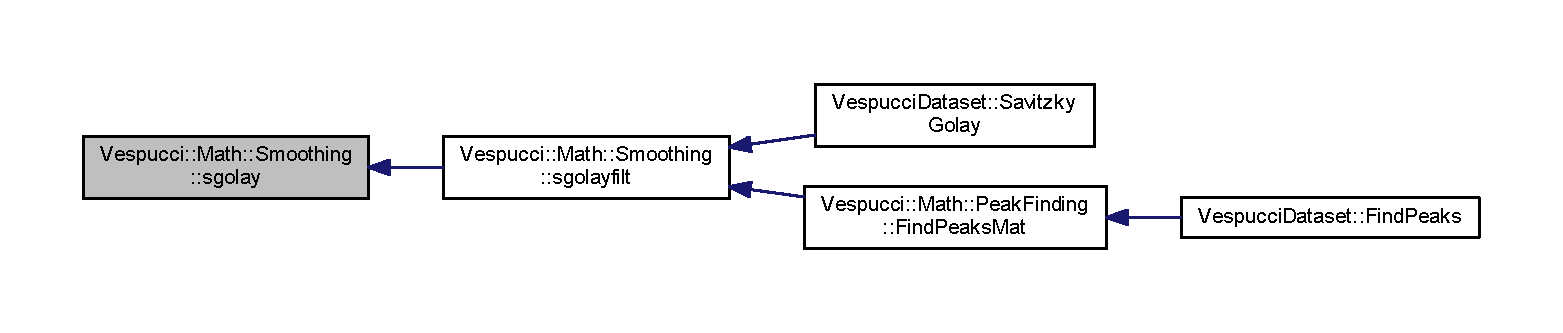
\includegraphics[width=350pt]{namespace_vespucci_1_1_math_1_1_smoothing_a0fb8087861e1d4b8f05dd4dff3cdb012_icgraph}
\end{center}
\end{figure}


\hypertarget{namespace_vespucci_1_1_math_1_1_smoothing_a2cb17f59d170c1ca2437b264d13626b6}{\index{Vespucci\+::\+Math\+::\+Smoothing@{Vespucci\+::\+Math\+::\+Smoothing}!sgolayfilt@{sgolayfilt}}
\index{sgolayfilt@{sgolayfilt}!Vespucci\+::\+Math\+::\+Smoothing@{Vespucci\+::\+Math\+::\+Smoothing}}
\subsubsection[{sgolayfilt}]{\setlength{\rightskip}{0pt plus 5cm}arma\+::mat Vespucci\+::\+Math\+::\+Smoothing\+::sgolayfilt (
\begin{DoxyParamCaption}
\item[{const arma\+::mat \&}]{x, }
\item[{arma\+::uword}]{poly\+\_\+order, }
\item[{arma\+::uword}]{window\+\_\+size, }
\item[{arma\+::uword}]{deriv\+\_\+order, }
\item[{arma\+::uword}]{scaling\+\_\+factor}
\end{DoxyParamCaption}
)}}\label{namespace_vespucci_1_1_math_1_1_smoothing_a2cb17f59d170c1ca2437b264d13626b6}


sgolayfilt Apply Savitzky-\/\+Golay smoothing to each column of a arma\+::matrix 


\begin{DoxyParams}{Parameters}
{\em x} & Input arma\+::matrix. Each column is a signal \\
\hline
{\em poly\+\_\+order} & Polynomial order for smoothing \\
\hline
{\em window\+\_\+size} & Size of filter window. Must be odd and larger than poly order \\
\hline
{\em deriv\+\_\+order} & Derivative order, to extract derivatized data directly \\
\hline
{\em scaling\+\_\+factor} & A scaling factor \\
\hline
\end{DoxyParams}
\begin{DoxyReturn}{Returns}
Smoothed data 
\end{DoxyReturn}


Definition at line 90 of file F\+I\+R.\+cpp.



Here is the call graph for this function\+:
\nopagebreak
\begin{figure}[H]
\begin{center}
\leavevmode
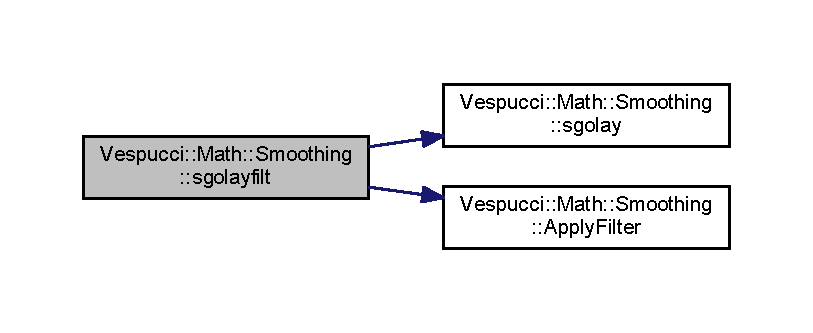
\includegraphics[width=350pt]{namespace_vespucci_1_1_math_1_1_smoothing_a2cb17f59d170c1ca2437b264d13626b6_cgraph}
\end{center}
\end{figure}




Here is the caller graph for this function\+:
\nopagebreak
\begin{figure}[H]
\begin{center}
\leavevmode
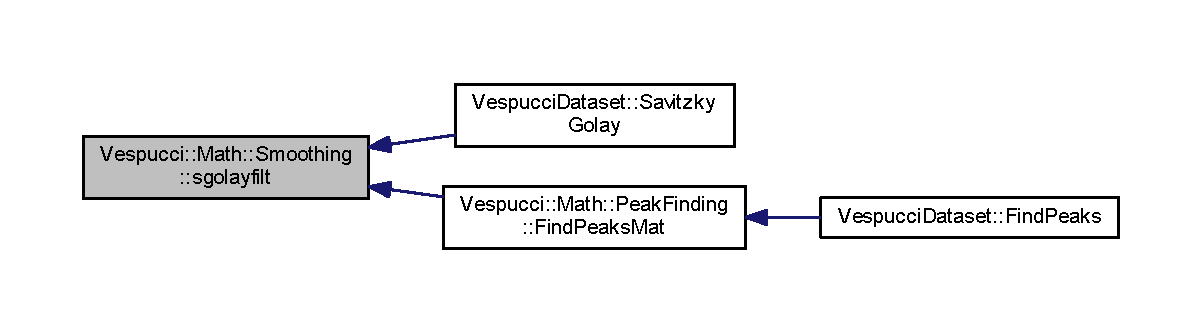
\includegraphics[width=350pt]{namespace_vespucci_1_1_math_1_1_smoothing_a2cb17f59d170c1ca2437b264d13626b6_icgraph}
\end{center}
\end{figure}


\hypertarget{namespace_vespucci_1_1_math_1_1_smoothing_ab92bb85566a363c2c54ad77d4eb2468f}{\index{Vespucci\+::\+Math\+::\+Smoothing@{Vespucci\+::\+Math\+::\+Smoothing}!Whittaker\+Smooth@{Whittaker\+Smooth}}
\index{Whittaker\+Smooth@{Whittaker\+Smooth}!Vespucci\+::\+Math\+::\+Smoothing@{Vespucci\+::\+Math\+::\+Smoothing}}
\subsubsection[{Whittaker\+Smooth}]{\setlength{\rightskip}{0pt plus 5cm}arma\+::vec Vespucci\+::\+Math\+::\+Smoothing\+::\+Whittaker\+Smooth (
\begin{DoxyParamCaption}
\item[{const arma\+::vec \&}]{x, }
\item[{double}]{lambda, }
\item[{arma\+::uword}]{penalty\+\_\+order}
\end{DoxyParamCaption}
)}}\label{namespace_vespucci_1_1_math_1_1_smoothing_ab92bb85566a363c2c54ad77d4eb2468f}


Vespucci\+::\+Math\+::\+Whittaker\+Smooth. 


\begin{DoxyParams}{Parameters}
{\em x} & \\
\hline
{\em lambda} & \\
\hline
{\em penalty\+\_\+order} & \\
\hline
\end{DoxyParams}
\begin{DoxyReturn}{Returns}
This may be re-\/written to use a sparse Cholesky decomposition if such a function comes to exist in armadillo or M\+L\+P\+A\+C\+K 
\end{DoxyReturn}


Definition at line 30 of file whittaker.\+cpp.



Here is the call graph for this function\+:
\nopagebreak
\begin{figure}[H]
\begin{center}
\leavevmode
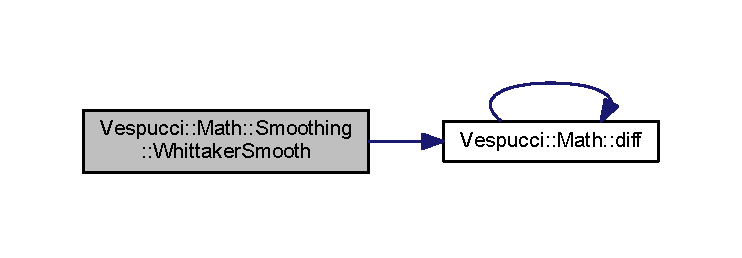
\includegraphics[width=350pt]{namespace_vespucci_1_1_math_1_1_smoothing_ab92bb85566a363c2c54ad77d4eb2468f_cgraph}
\end{center}
\end{figure}



\chapter{Class Documentation}
\hypertarget{class_about_dialog}{\section{About\+Dialog Class Reference}
\label{class_about_dialog}\index{About\+Dialog@{About\+Dialog}}
}


The \hyperlink{class_about_dialog}{About\+Dialog} class A Q\+Dialog that displays information about \hyperlink{namespace_vespucci}{Vespucci}.  




{\ttfamily \#include $<$aboutdialog.\+h$>$}



Inheritance diagram for About\+Dialog\+:\nopagebreak
\begin{figure}[H]
\begin{center}
\leavevmode
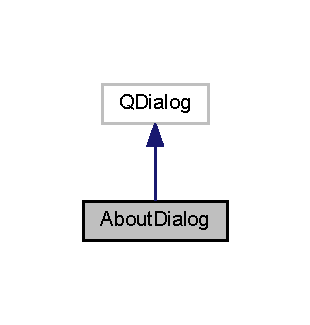
\includegraphics[width=149pt]{class_about_dialog__inherit__graph}
\end{center}
\end{figure}


Collaboration diagram for About\+Dialog\+:\nopagebreak
\begin{figure}[H]
\begin{center}
\leavevmode
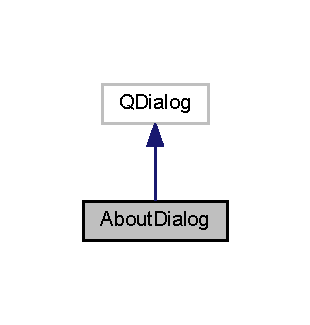
\includegraphics[width=149pt]{class_about_dialog__coll__graph}
\end{center}
\end{figure}
\subsection*{Public Member Functions}
\begin{DoxyCompactItemize}
\item 
\hypertarget{class_about_dialog_ad96fc2ce8de7568ace543b7c69c71c56}{{\bfseries About\+Dialog} (Q\+Widget $\ast$parent=0)}\label{class_about_dialog_ad96fc2ce8de7568ace543b7c69c71c56}

\end{DoxyCompactItemize}


\subsection{Detailed Description}
The \hyperlink{class_about_dialog}{About\+Dialog} class A Q\+Dialog that displays information about \hyperlink{namespace_vespucci}{Vespucci}. 

Definition at line 31 of file aboutdialog.\+h.



The documentation for this class was generated from the following files\+:\begin{DoxyCompactItemize}
\item 
C\+:/\+Projects/\+Vespucci/develop/\+G\+U\+I/\+Display/aboutdialog.\+h\item 
C\+:/\+Projects/\+Vespucci/develop/\+G\+U\+I/\+Display/aboutdialog.\+cpp\end{DoxyCompactItemize}

\hypertarget{class_analysis_dialog}{\section{Analysis\+Dialog Class Reference}
\label{class_analysis_dialog}\index{Analysis\+Dialog@{Analysis\+Dialog}}
}


Inheritance diagram for Analysis\+Dialog\+:\nopagebreak
\begin{figure}[H]
\begin{center}
\leavevmode
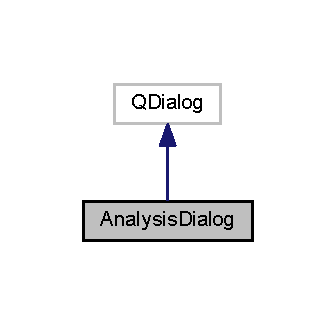
\includegraphics[width=161pt]{class_analysis_dialog__inherit__graph}
\end{center}
\end{figure}


Collaboration diagram for Analysis\+Dialog\+:\nopagebreak
\begin{figure}[H]
\begin{center}
\leavevmode
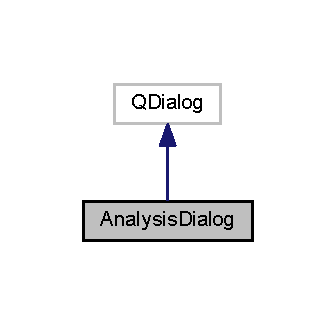
\includegraphics[width=161pt]{class_analysis_dialog__coll__graph}
\end{center}
\end{figure}
\subsection*{Public Member Functions}
\begin{DoxyCompactItemize}
\item 
\hypertarget{class_analysis_dialog_a74170aa9e6cabf4154cedf788a31f755}{{\bfseries Analysis\+Dialog} (Q\+Widget $\ast$parent, \hyperlink{class_vespucci_workspace}{Vespucci\+Workspace} $\ast$ws, int row)}\label{class_analysis_dialog_a74170aa9e6cabf4154cedf788a31f755}

\end{DoxyCompactItemize}


\subsection{Detailed Description}


Definition at line 30 of file analysisdialog.\+h.



The documentation for this class was generated from the following files\+:\begin{DoxyCompactItemize}
\item 
C\+:/\+Projects/\+Vespucci/develop/\+G\+U\+I/\+Analysis/analysisdialog.\+h\item 
C\+:/\+Projects/\+Vespucci/develop/\+G\+U\+I/\+Analysis/analysisdialog.\+cpp\end{DoxyCompactItemize}

\hypertarget{class_analysis_results}{\section{Analysis\+Results Class Reference}
\label{class_analysis_results}\index{Analysis\+Results@{Analysis\+Results}}
}


The \hyperlink{class_analysis_results}{Analysis\+Results} class A container for a mat object that allows a mat to be copied to a heap-\/allocated object (this) so pointers to that mat cannot go out of scope. These objects should be heap-\/allocated inside smart pointers.  




{\ttfamily \#include $<$analysisresults.\+h$>$}

\subsection*{Public Member Functions}
\begin{DoxyCompactItemize}
\item 
\hypertarget{class_analysis_results_a96290e00cecee6d9fea02ffb42633eeb}{{\bfseries Analysis\+Results} (mat value)}\label{class_analysis_results_a96290e00cecee6d9fea02ffb42633eeb}

\item 
\hypertarget{class_analysis_results_ae591750de59fc7c4a8bcb9d422cf161d}{mat {\bfseries value} ()}\label{class_analysis_results_ae591750de59fc7c4a8bcb9d422cf161d}

\item 
\hypertarget{class_analysis_results_a1ea6245771f569a72f0cccae21798270}{mat $\ast$ {\bfseries value\+\_\+ptr} ()}\label{class_analysis_results_a1ea6245771f569a72f0cccae21798270}

\end{DoxyCompactItemize}


\subsection{Detailed Description}
The \hyperlink{class_analysis_results}{Analysis\+Results} class A container for a mat object that allows a mat to be copied to a heap-\/allocated object (this) so pointers to that mat cannot go out of scope. These objects should be heap-\/allocated inside smart pointers. 

Definition at line 29 of file analysisresults.\+h.



The documentation for this class was generated from the following files\+:\begin{DoxyCompactItemize}
\item 
C\+:/\+Projects/\+Vespucci/develop/\+Data/\+Analysis/analysisresults.\+h\item 
C\+:/\+Projects/\+Vespucci/develop/\+Data/\+Analysis/analysisresults.\+cpp\end{DoxyCompactItemize}

\hypertarget{class_band_ratio_dialog}{\section{Band\+Ratio\+Dialog Class Reference}
\label{class_band_ratio_dialog}\index{Band\+Ratio\+Dialog@{Band\+Ratio\+Dialog}}
}


The \hyperlink{class_band_ratio_dialog}{Band\+Ratio\+Dialog} class The dialog that allows the user to create a band-\/ratio map.  




{\ttfamily \#include $<$bandratiodialog.\+h$>$}



Inheritance diagram for Band\+Ratio\+Dialog\+:\nopagebreak
\begin{figure}[H]
\begin{center}
\leavevmode
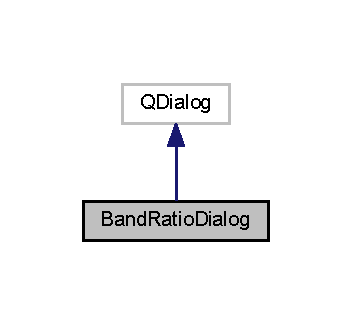
\includegraphics[width=169pt]{class_band_ratio_dialog__inherit__graph}
\end{center}
\end{figure}


Collaboration diagram for Band\+Ratio\+Dialog\+:\nopagebreak
\begin{figure}[H]
\begin{center}
\leavevmode
\includegraphics[width=169pt]{class_band_ratio_dialog__coll__graph}
\end{center}
\end{figure}
\subsection*{Public Member Functions}
\begin{DoxyCompactItemize}
\item 
\hypertarget{class_band_ratio_dialog_a9f8135f338936413f8a02e149e95df0a}{{\bfseries Band\+Ratio\+Dialog} (Q\+Widget $\ast$parent, \hyperlink{class_vespucci_workspace}{Vespucci\+Workspace} $\ast$ws, int row)}\label{class_band_ratio_dialog_a9f8135f338936413f8a02e149e95df0a}

\end{DoxyCompactItemize}


\subsection{Detailed Description}
The \hyperlink{class_band_ratio_dialog}{Band\+Ratio\+Dialog} class The dialog that allows the user to create a band-\/ratio map. 

Definition at line 34 of file bandratiodialog.\+h.



The documentation for this class was generated from the following files\+:\begin{DoxyCompactItemize}
\item 
C\+:/\+Projects/\+Vespucci/develop/\+G\+U\+I/\+Analysis/bandratiodialog.\+h\item 
C\+:/\+Projects/\+Vespucci/develop/\+G\+U\+I/\+Analysis/bandratiodialog.\+cpp\end{DoxyCompactItemize}

\hypertarget{class_baseline_dialog}{\section{Baseline\+Dialog Class Reference}
\label{class_baseline_dialog}\index{Baseline\+Dialog@{Baseline\+Dialog}}
}


The \hyperlink{class_baseline_dialog}{Baseline\+Dialog} class The dialog that allows the user to baseline-\/correct the data.  




{\ttfamily \#include $<$baselinedialog.\+h$>$}



Inheritance diagram for Baseline\+Dialog\+:\nopagebreak
\begin{figure}[H]
\begin{center}
\leavevmode
\includegraphics[width=161pt]{class_baseline_dialog__inherit__graph}
\end{center}
\end{figure}


Collaboration diagram for Baseline\+Dialog\+:\nopagebreak
\begin{figure}[H]
\begin{center}
\leavevmode
\includegraphics[width=161pt]{class_baseline_dialog__coll__graph}
\end{center}
\end{figure}
\subsection*{Public Member Functions}
\begin{DoxyCompactItemize}
\item 
\hyperlink{class_baseline_dialog_a6feebcff1d6286f5e8c0eec4fd35f738}{Baseline\+Dialog} (Q\+Widget $\ast$parent, \hyperlink{class_vespucci_workspace}{Vespucci\+Workspace} $\ast$ws, int row)
\begin{DoxyCompactList}\small\item\em \hyperlink{class_baseline_dialog_a6feebcff1d6286f5e8c0eec4fd35f738}{Baseline\+Dialog\+::\+Baseline\+Dialog}. \end{DoxyCompactList}\end{DoxyCompactItemize}


\subsection{Detailed Description}
The \hyperlink{class_baseline_dialog}{Baseline\+Dialog} class The dialog that allows the user to baseline-\/correct the data. 

Definition at line 34 of file baselinedialog.\+h.



\subsection{Constructor \& Destructor Documentation}
\hypertarget{class_baseline_dialog_a6feebcff1d6286f5e8c0eec4fd35f738}{\index{Baseline\+Dialog@{Baseline\+Dialog}!Baseline\+Dialog@{Baseline\+Dialog}}
\index{Baseline\+Dialog@{Baseline\+Dialog}!Baseline\+Dialog@{Baseline\+Dialog}}
\subsubsection[{Baseline\+Dialog}]{\setlength{\rightskip}{0pt plus 5cm}Baseline\+Dialog\+::\+Baseline\+Dialog (
\begin{DoxyParamCaption}
\item[{Q\+Widget $\ast$}]{parent, }
\item[{{\bf Vespucci\+Workspace} $\ast$}]{ws, }
\item[{int}]{row}
\end{DoxyParamCaption}
)\hspace{0.3cm}{\ttfamily [explicit]}}}\label{class_baseline_dialog_a6feebcff1d6286f5e8c0eec4fd35f738}


\hyperlink{class_baseline_dialog_a6feebcff1d6286f5e8c0eec4fd35f738}{Baseline\+Dialog\+::\+Baseline\+Dialog}. 


\begin{DoxyParams}{Parameters}
{\em parent} & Parent widget, required for Q\+Dialog \\
\hline
{\em ws} & The current workspace \\
\hline
{\em row} & The currently selected row in the dataset list widget \\
\hline
\end{DoxyParams}


Definition at line 29 of file baselinedialog.\+cpp.



Here is the call graph for this function\+:\nopagebreak
\begin{figure}[H]
\begin{center}
\leavevmode
\includegraphics[width=350pt]{class_baseline_dialog_a6feebcff1d6286f5e8c0eec4fd35f738_cgraph}
\end{center}
\end{figure}




The documentation for this class was generated from the following files\+:\begin{DoxyCompactItemize}
\item 
C\+:/\+Projects/\+Vespucci/develop/\+G\+U\+I/\+Processing/baselinedialog.\+h\item 
C\+:/\+Projects/\+Vespucci/develop/\+G\+U\+I/\+Processing/baselinedialog.\+cpp\end{DoxyCompactItemize}

\hypertarget{class_booleanize_dialog}{\section{Booleanize\+Dialog Class Reference}
\label{class_booleanize_dialog}\index{Booleanize\+Dialog@{Booleanize\+Dialog}}
}


Inheritance diagram for Booleanize\+Dialog\+:\nopagebreak
\begin{figure}[H]
\begin{center}
\leavevmode
\includegraphics[width=172pt]{class_booleanize_dialog__inherit__graph}
\end{center}
\end{figure}


Collaboration diagram for Booleanize\+Dialog\+:\nopagebreak
\begin{figure}[H]
\begin{center}
\leavevmode
\includegraphics[width=172pt]{class_booleanize_dialog__coll__graph}
\end{center}
\end{figure}
\subsection*{Public Member Functions}
\begin{DoxyCompactItemize}
\item 
\hypertarget{class_booleanize_dialog_aae68d3541d225de9c90c8f5a128c7027}{{\bfseries Booleanize\+Dialog} (Q\+Widget $\ast$parent, \hyperlink{class_vespucci_workspace}{Vespucci\+Workspace} $\ast$ws, int row)}\label{class_booleanize_dialog_aae68d3541d225de9c90c8f5a128c7027}

\end{DoxyCompactItemize}


\subsection{Detailed Description}


Definition at line 12 of file booleanizedialog.\+h.



The documentation for this class was generated from the following files\+:\begin{DoxyCompactItemize}
\item 
C\+:/\+Projects/\+Vespucci/develop/\+G\+U\+I/\+Processing/booleanizedialog.\+h\item 
C\+:/\+Projects/\+Vespucci/develop/\+G\+U\+I/\+Processing/booleanizedialog.\+cpp\end{DoxyCompactItemize}

\hypertarget{class_citation_dialog}{\section{Citation\+Dialog Class Reference}
\label{class_citation_dialog}\index{Citation\+Dialog@{Citation\+Dialog}}
}


The \hyperlink{class_citation_dialog}{Citation\+Dialog} class The dialog that displays how to cite \hyperlink{namespace_vespucci}{Vespucci}.  




{\ttfamily \#include $<$citationdialog.\+h$>$}



Inheritance diagram for Citation\+Dialog\+:\nopagebreak
\begin{figure}[H]
\begin{center}
\leavevmode
\includegraphics[width=157pt]{class_citation_dialog__inherit__graph}
\end{center}
\end{figure}


Collaboration diagram for Citation\+Dialog\+:\nopagebreak
\begin{figure}[H]
\begin{center}
\leavevmode
\includegraphics[width=157pt]{class_citation_dialog__coll__graph}
\end{center}
\end{figure}
\subsection*{Public Member Functions}
\begin{DoxyCompactItemize}
\item 
\hyperlink{class_citation_dialog_a566d6d063e20f68d619ff15412bda2f0}{Citation\+Dialog} (Q\+Widget $\ast$parent=0)
\begin{DoxyCompactList}\small\item\em \hyperlink{class_citation_dialog_a566d6d063e20f68d619ff15412bda2f0}{Citation\+Dialog\+::\+Citation\+Dialog}. \end{DoxyCompactList}\end{DoxyCompactItemize}


\subsection{Detailed Description}
The \hyperlink{class_citation_dialog}{Citation\+Dialog} class The dialog that displays how to cite \hyperlink{namespace_vespucci}{Vespucci}. 

Definition at line 32 of file citationdialog.\+h.



\subsection{Constructor \& Destructor Documentation}
\hypertarget{class_citation_dialog_a566d6d063e20f68d619ff15412bda2f0}{\index{Citation\+Dialog@{Citation\+Dialog}!Citation\+Dialog@{Citation\+Dialog}}
\index{Citation\+Dialog@{Citation\+Dialog}!Citation\+Dialog@{Citation\+Dialog}}
\subsubsection[{Citation\+Dialog}]{\setlength{\rightskip}{0pt plus 5cm}Citation\+Dialog\+::\+Citation\+Dialog (
\begin{DoxyParamCaption}
\item[{Q\+Widget $\ast$}]{parent = {\ttfamily 0}}
\end{DoxyParamCaption}
)\hspace{0.3cm}{\ttfamily [explicit]}}}\label{class_citation_dialog_a566d6d063e20f68d619ff15412bda2f0}


\hyperlink{class_citation_dialog_a566d6d063e20f68d619ff15412bda2f0}{Citation\+Dialog\+::\+Citation\+Dialog}. 


\begin{DoxyParams}{Parameters}
{\em parent} & Parent Q\+Widget, common for all Q\+Dialogs \\
\hline
\end{DoxyParams}


Definition at line 27 of file citationdialog.\+cpp.



The documentation for this class was generated from the following files\+:\begin{DoxyCompactItemize}
\item 
C\+:/\+Projects/\+Vespucci/develop/\+G\+U\+I/\+Display/citationdialog.\+h\item 
C\+:/\+Projects/\+Vespucci/develop/\+G\+U\+I/\+Display/citationdialog.\+cpp\end{DoxyCompactItemize}

\hypertarget{class_crop_dialog}{\section{Crop\+Dialog Class Reference}
\label{class_crop_dialog}\index{Crop\+Dialog@{Crop\+Dialog}}
}


The \hyperlink{class_crop_dialog}{Crop\+Dialog} class A dialog that allows the user to \char`\"{}\+Crop\char`\"{} the dataset (delete all spectra that are outside of a chosen spatial range).  




{\ttfamily \#include $<$cropdialog.\+h$>$}



Inheritance diagram for Crop\+Dialog\+:\nopagebreak
\begin{figure}[H]
\begin{center}
\leavevmode
\includegraphics[width=144pt]{class_crop_dialog__inherit__graph}
\end{center}
\end{figure}


Collaboration diagram for Crop\+Dialog\+:\nopagebreak
\begin{figure}[H]
\begin{center}
\leavevmode
\includegraphics[width=144pt]{class_crop_dialog__coll__graph}
\end{center}
\end{figure}
\subsection*{Public Member Functions}
\begin{DoxyCompactItemize}
\item 
\hyperlink{class_crop_dialog_aecf1b569a29c94fe0678a6d352c31740}{Crop\+Dialog} (Q\+Widget $\ast$parent, \hyperlink{class_vespucci_workspace}{Vespucci\+Workspace} $\ast$ws, int row)
\begin{DoxyCompactList}\small\item\em \hyperlink{class_crop_dialog_aecf1b569a29c94fe0678a6d352c31740}{Crop\+Dialog\+::\+Crop\+Dialog}. \end{DoxyCompactList}\end{DoxyCompactItemize}


\subsection{Detailed Description}
The \hyperlink{class_crop_dialog}{Crop\+Dialog} class A dialog that allows the user to \char`\"{}\+Crop\char`\"{} the dataset (delete all spectra that are outside of a chosen spatial range). 

Definition at line 35 of file cropdialog.\+h.



\subsection{Constructor \& Destructor Documentation}
\hypertarget{class_crop_dialog_aecf1b569a29c94fe0678a6d352c31740}{\index{Crop\+Dialog@{Crop\+Dialog}!Crop\+Dialog@{Crop\+Dialog}}
\index{Crop\+Dialog@{Crop\+Dialog}!Crop\+Dialog@{Crop\+Dialog}}
\subsubsection[{Crop\+Dialog}]{\setlength{\rightskip}{0pt plus 5cm}Crop\+Dialog\+::\+Crop\+Dialog (
\begin{DoxyParamCaption}
\item[{Q\+Widget $\ast$}]{parent, }
\item[{{\bf Vespucci\+Workspace} $\ast$}]{ws, }
\item[{int}]{row}
\end{DoxyParamCaption}
)\hspace{0.3cm}{\ttfamily [explicit]}}}\label{class_crop_dialog_aecf1b569a29c94fe0678a6d352c31740}


\hyperlink{class_crop_dialog_aecf1b569a29c94fe0678a6d352c31740}{Crop\+Dialog\+::\+Crop\+Dialog}. 


\begin{DoxyParams}{Parameters}
{\em parent} & Parent Q\+Widget \\
\hline
{\em ws} & The current workspace \\
\hline
{\em row} & Currently selected row \\
\hline
\end{DoxyParams}


Definition at line 31 of file cropdialog.\+cpp.



Here is the call graph for this function\+:\nopagebreak
\begin{figure}[H]
\begin{center}
\leavevmode
\includegraphics[width=346pt]{class_crop_dialog_aecf1b569a29c94fe0678a6d352c31740_cgraph}
\end{center}
\end{figure}




The documentation for this class was generated from the following files\+:\begin{DoxyCompactItemize}
\item 
C\+:/\+Projects/\+Vespucci/develop/\+G\+U\+I/\+Processing/cropdialog.\+h\item 
C\+:/\+Projects/\+Vespucci/develop/\+G\+U\+I/\+Processing/cropdialog.\+cpp\end{DoxyCompactItemize}

\hypertarget{class_c_w_t_data}{\section{C\+W\+T\+Data Class Reference}
\label{class_c_w_t_data}\index{C\+W\+T\+Data@{C\+W\+T\+Data}}
}
\subsection*{Public Member Functions}
\begin{DoxyCompactItemize}
\item 
\hypertarget{class_c_w_t_data_ae3a109688cea3f935d866eb14bdd5040}{{\bfseries C\+W\+T\+Data} (Q\+Shared\+Pointer$<$ \hyperlink{class_vespucci_dataset}{Vespucci\+Dataset} $>$ dataset)}\label{class_c_w_t_data_ae3a109688cea3f935d866eb14bdd5040}

\item 
void \hyperlink{class_c_w_t_data_a2bef5240e7e285a722170a79ec09d326}{Apply} (std\+::string wavelet=\char`\"{}mexh\char`\"{}, uword max\+\_\+scale=70, uword gap\+\_\+threshold=3, uword min\+\_\+ridge\+\_\+length=5, uword search\+\_\+width=5, double noise\+\_\+threshold=3.\+0, std\+::string noise\+\_\+method=\char`\"{}quantile\char`\"{}, uword noise\+\_\+window\+\_\+size=500, bool save\+\_\+coefs=false, bool save\+\_\+coef\+\_\+plots=false, bool save\+\_\+ridge\+\_\+plots=false, bool save\+\_\+ridge\+\_\+plot\+\_\+data=false, bool estimate\+\_\+width=false, Q\+String save\+\_\+directory=\char`\"{}C\+W\+T Data\char`\"{}, Q\+String image\+\_\+format=\char`\"{}pdf\char`\"{}, Q\+C\+P\+Color\+Gradient gradient=Q\+C\+P\+Color\+Gradient\+::cb\+Greys)
\begin{DoxyCompactList}\small\item\em \hyperlink{class_c_w_t_data_a2bef5240e7e285a722170a79ec09d326}{C\+W\+T\+Data\+::\+Apply}. \end{DoxyCompactList}\item 
mat \hyperlink{class_c_w_t_data_ad5f5f9db597ab00373481e6067ba75ac}{centers} ()
\begin{DoxyCompactList}\small\item\em \hyperlink{class_c_w_t_data_ad5f5f9db597ab00373481e6067ba75ac}{C\+W\+T\+Data\+::centers}. \end{DoxyCompactList}\item 
\hypertarget{class_c_w_t_data_a95b94433d6244a37cdee0205a67b0321}{void \hyperlink{class_c_w_t_data_a95b94433d6244a37cdee0205a67b0321}{clear} ()}\label{class_c_w_t_data_a95b94433d6244a37cdee0205a67b0321}

\begin{DoxyCompactList}\small\item\em \hyperlink{class_c_w_t_data_a95b94433d6244a37cdee0205a67b0321}{C\+W\+T\+Data\+::clear} Delete everything in peak\+\_\+data\+\_\+. \end{DoxyCompactList}\item 
mat \hyperlink{class_c_w_t_data_a829d9ca8cdabff46dd3654f2bda64899}{counts} () const 
\begin{DoxyCompactList}\small\item\em \hyperlink{class_c_w_t_data_a829d9ca8cdabff46dd3654f2bda64899}{C\+W\+T\+Data\+::counts}. \end{DoxyCompactList}\item 
mat \hyperlink{class_c_w_t_data_acfc35d0f61d67aedc7bf2fed91de1319}{Has\+Peaks} (const mat \&range\+\_\+list)
\begin{DoxyCompactList}\small\item\em \hyperlink{class_c_w_t_data_acfc35d0f61d67aedc7bf2fed91de1319}{C\+W\+T\+Data\+::\+Has\+Peaks}. \end{DoxyCompactList}\end{DoxyCompactItemize}


\subsection{Detailed Description}


Definition at line 10 of file cwtdata.\+h.



\subsection{Member Function Documentation}
\hypertarget{class_c_w_t_data_a2bef5240e7e285a722170a79ec09d326}{\index{C\+W\+T\+Data@{C\+W\+T\+Data}!Apply@{Apply}}
\index{Apply@{Apply}!C\+W\+T\+Data@{C\+W\+T\+Data}}
\subsubsection[{Apply}]{\setlength{\rightskip}{0pt plus 5cm}void C\+W\+T\+Data\+::\+Apply (
\begin{DoxyParamCaption}
\item[{std\+::string}]{wavelet = {\ttfamily \char`\"{}mexh\char`\"{}}, }
\item[{uword}]{max\+\_\+scale = {\ttfamily 70}, }
\item[{uword}]{gap\+\_\+threshold = {\ttfamily 3}, }
\item[{uword}]{min\+\_\+ridge\+\_\+length = {\ttfamily 5}, }
\item[{uword}]{search\+\_\+width = {\ttfamily 5}, }
\item[{double}]{noise\+\_\+threshold = {\ttfamily 3.0}, }
\item[{std\+::string}]{noise\+\_\+method = {\ttfamily \char`\"{}quantile\char`\"{}}, }
\item[{uword}]{noise\+\_\+window\+\_\+size = {\ttfamily 500}, }
\item[{bool}]{save\+\_\+coefs = {\ttfamily false}, }
\item[{bool}]{save\+\_\+coef\+\_\+plots = {\ttfamily false}, }
\item[{bool}]{save\+\_\+ridge\+\_\+plots = {\ttfamily false}, }
\item[{bool}]{save\+\_\+ridge\+\_\+plot\+\_\+data = {\ttfamily false}, }
\item[{bool}]{estimate\+\_\+width = {\ttfamily false}, }
\item[{Q\+String}]{save\+\_\+directory = {\ttfamily \char`\"{}CWT~Data\char`\"{}}, }
\item[{Q\+String}]{image\+\_\+format = {\ttfamily \char`\"{}pdf\char`\"{}}, }
\item[{Q\+C\+P\+Color\+Gradient}]{gradient = {\ttfamily QCPColorGradient\+:\+:cbGreys}}
\end{DoxyParamCaption}
)}}\label{class_c_w_t_data_a2bef5240e7e285a722170a79ec09d326}


\hyperlink{class_c_w_t_data_a2bef5240e7e285a722170a79ec09d326}{C\+W\+T\+Data\+::\+Apply}. 


\begin{DoxyParams}{Parameters}
{\em wavelet} & \\
\hline
{\em max\+\_\+scale} & \\
\hline
{\em gap\+\_\+threshold} & \\
\hline
{\em min\+\_\+ridge\+\_\+length} & \\
\hline
{\em search\+\_\+width} & \\
\hline
{\em noise\+\_\+threshold} & \\
\hline
{\em noise\+\_\+method} & \\
\hline
{\em noise\+\_\+window\+\_\+size} & \\
\hline
{\em save\+\_\+coefs} & \\
\hline
{\em save\+\_\+coef\+\_\+plots} & \\
\hline
{\em save\+\_\+ridge\+\_\+plots} & \\
\hline
{\em save\+\_\+ridge\+\_\+plot\+\_\+data} & \\
\hline
{\em save\+\_\+directory} & \\
\hline
\end{DoxyParams}


Definition at line 24 of file cwtdata.\+cpp.



Here is the call graph for this function\+:
\nopagebreak
\begin{figure}[H]
\begin{center}
\leavevmode
\includegraphics[width=350pt]{class_c_w_t_data_a2bef5240e7e285a722170a79ec09d326_cgraph}
\end{center}
\end{figure}


\hypertarget{class_c_w_t_data_ad5f5f9db597ab00373481e6067ba75ac}{\index{C\+W\+T\+Data@{C\+W\+T\+Data}!centers@{centers}}
\index{centers@{centers}!C\+W\+T\+Data@{C\+W\+T\+Data}}
\subsubsection[{centers}]{\setlength{\rightskip}{0pt plus 5cm}mat C\+W\+T\+Data\+::centers (
\begin{DoxyParamCaption}
{}
\end{DoxyParamCaption}
)}}\label{class_c_w_t_data_ad5f5f9db597ab00373481e6067ba75ac}


\hyperlink{class_c_w_t_data_ad5f5f9db597ab00373481e6067ba75ac}{C\+W\+T\+Data\+::centers}. 

\begin{DoxyReturn}{Returns}
A single matrix containing a summary of the information in peak\+\_\+data\+\_\+ This is intended to be called once and that matrix stored as an Analysis\+Result to be viewed in the data viewer. 
\end{DoxyReturn}


Definition at line 256 of file cwtdata.\+cpp.



Here is the call graph for this function\+:
\nopagebreak
\begin{figure}[H]
\begin{center}
\leavevmode
\includegraphics[width=350pt]{class_c_w_t_data_ad5f5f9db597ab00373481e6067ba75ac_cgraph}
\end{center}
\end{figure}


\hypertarget{class_c_w_t_data_a829d9ca8cdabff46dd3654f2bda64899}{\index{C\+W\+T\+Data@{C\+W\+T\+Data}!counts@{counts}}
\index{counts@{counts}!C\+W\+T\+Data@{C\+W\+T\+Data}}
\subsubsection[{counts}]{\setlength{\rightskip}{0pt plus 5cm}mat C\+W\+T\+Data\+::counts (
\begin{DoxyParamCaption}
{}
\end{DoxyParamCaption}
) const}}\label{class_c_w_t_data_a829d9ca8cdabff46dd3654f2bda64899}


\hyperlink{class_c_w_t_data_a829d9ca8cdabff46dd3654f2bda64899}{C\+W\+T\+Data\+::counts}. 

\begin{DoxyReturn}{Returns}
The matrix describing the counts of peaks at each center 
\end{DoxyReturn}


Definition at line 346 of file cwtdata.\+cpp.

\hypertarget{class_c_w_t_data_acfc35d0f61d67aedc7bf2fed91de1319}{\index{C\+W\+T\+Data@{C\+W\+T\+Data}!Has\+Peaks@{Has\+Peaks}}
\index{Has\+Peaks@{Has\+Peaks}!C\+W\+T\+Data@{C\+W\+T\+Data}}
\subsubsection[{Has\+Peaks}]{\setlength{\rightskip}{0pt plus 5cm}mat C\+W\+T\+Data\+::\+Has\+Peaks (
\begin{DoxyParamCaption}
\item[{const mat \&}]{range\+\_\+list}
\end{DoxyParamCaption}
)}}\label{class_c_w_t_data_acfc35d0f61d67aedc7bf2fed91de1319}


\hyperlink{class_c_w_t_data_acfc35d0f61d67aedc7bf2fed91de1319}{C\+W\+T\+Data\+::\+Has\+Peaks}. 


\begin{DoxyParams}{Parameters}
{\em range\+\_\+list} & A matrix where each row consists of a left and right bound to determine whether or not a peak center was found in that range. \\
\hline
\end{DoxyParams}
\begin{DoxyReturn}{Returns}
A matrix with the number of rows equal to the rows of the dataset when this object was created. Each column corresponds to a requested range. 
\end{DoxyReturn}


Definition at line 358 of file cwtdata.\+cpp.



The documentation for this class was generated from the following files\+:\begin{DoxyCompactItemize}
\item 
C\+:/\+Projects/\+Vespucci/develop/\+Data/\+Analysis/cwtdata.\+h\item 
C\+:/\+Projects/\+Vespucci/develop/\+Data/\+Analysis/cwtdata.\+cpp\end{DoxyCompactItemize}

\hypertarget{class_vespucci_1_1_math_1_1_c_w_t_ridge}{\section{Vespucci\+:\+:Math\+:\+:C\+W\+T\+Ridge Class Reference}
\label{class_vespucci_1_1_math_1_1_c_w_t_ridge}\index{Vespucci\+::\+Math\+::\+C\+W\+T\+Ridge@{Vespucci\+::\+Math\+::\+C\+W\+T\+Ridge}}
}
\subsection*{Public Member Functions}
\begin{DoxyCompactItemize}
\item 
\hypertarget{class_vespucci_1_1_math_1_1_c_w_t_ridge_abc64696867de953935fb7752eb7aa3c5}{{\bfseries C\+W\+T\+Ridge} (int id)}\label{class_vespucci_1_1_math_1_1_c_w_t_ridge_abc64696867de953935fb7752eb7aa3c5}

\item 
\hypertarget{class_vespucci_1_1_math_1_1_c_w_t_ridge_a9cb96470fb5099fb484f785b03062a61}{arma\+::umat {\bfseries points} () const }\label{class_vespucci_1_1_math_1_1_c_w_t_ridge_a9cb96470fb5099fb484f785b03062a61}

\item 
arma\+::uword \hyperlink{class_vespucci_1_1_math_1_1_c_w_t_ridge_a83f1ff9fd6e95fb8208055c27e10f1fb}{gap} () const 
\begin{DoxyCompactList}\small\item\em \hyperlink{class_vespucci_1_1_math_1_1_c_w_t_ridge_a83f1ff9fd6e95fb8208055c27e10f1fb}{Vespucci\+::\+Math\+::\+C\+W\+T\+Ridge\+::gap}. \end{DoxyCompactList}\item 
bool \hyperlink{class_vespucci_1_1_math_1_1_c_w_t_ridge_a9057997bb1df3b32bfc85e75784961f2}{Has\+Point} (arma\+::uword row, arma\+::uword column) const 
\begin{DoxyCompactList}\small\item\em \hyperlink{class_vespucci_1_1_math_1_1_c_w_t_ridge_a9057997bb1df3b32bfc85e75784961f2}{Vespucci\+::\+Math\+::\+C\+W\+T\+Ridge\+::\+Has\+Point}. \end{DoxyCompactList}\item 
arma\+::uword \hyperlink{class_vespucci_1_1_math_1_1_c_w_t_ridge_a79079be89121582e51a8bae224434c7f}{scale} () const 
\begin{DoxyCompactList}\small\item\em \hyperlink{class_vespucci_1_1_math_1_1_c_w_t_ridge_a79079be89121582e51a8bae224434c7f}{Vespucci\+::\+Math\+::\+C\+W\+T\+Ridge\+::scale}. \end{DoxyCompactList}\item 
void \hyperlink{class_vespucci_1_1_math_1_1_c_w_t_ridge_a0cdb8e92d9b1d1fba2aef32ea882813a}{Insert\+Point} (arma\+::uword row, arma\+::uword column, double \hyperlink{class_vespucci_1_1_math_1_1_c_w_t_ridge_a58ed7b3dc07c568c93daeb266f8b7e56}{value})
\begin{DoxyCompactList}\small\item\em \hyperlink{class_vespucci_1_1_math_1_1_c_w_t_ridge_a0cdb8e92d9b1d1fba2aef32ea882813a}{Vespucci\+::\+Math\+::\+C\+W\+T\+Ridge\+::\+Insert\+Point}. \end{DoxyCompactList}\item 
\hypertarget{class_vespucci_1_1_math_1_1_c_w_t_ridge_a3eeb78c61242936900bcf1497a2d4c17}{void {\bfseries Merge} (\hyperlink{class_vespucci_1_1_math_1_1_c_w_t_ridge}{C\+W\+T\+Ridge} \&new\+\_\+ridge)}\label{class_vespucci_1_1_math_1_1_c_w_t_ridge_a3eeb78c61242936900bcf1497a2d4c17}

\item 
\hypertarget{class_vespucci_1_1_math_1_1_c_w_t_ridge_a039fef6b6678664d8bb8c019937bfbf9}{void \hyperlink{class_vespucci_1_1_math_1_1_c_w_t_ridge_a039fef6b6678664d8bb8c019937bfbf9}{Remove\+Last\+Point} ()}\label{class_vespucci_1_1_math_1_1_c_w_t_ridge_a039fef6b6678664d8bb8c019937bfbf9}

\begin{DoxyCompactList}\small\item\em \hyperlink{class_vespucci_1_1_math_1_1_c_w_t_ridge_a039fef6b6678664d8bb8c019937bfbf9}{Vespucci\+::\+Math\+::\+C\+W\+T\+Ridge\+::\+Remove\+Last\+Point} remove the last added point (in case gap is too high) \end{DoxyCompactList}\item 
double \hyperlink{class_vespucci_1_1_math_1_1_c_w_t_ridge_a58ed7b3dc07c568c93daeb266f8b7e56}{value} (arma\+::uword row, arma\+::uword column) const 
\begin{DoxyCompactList}\small\item\em \hyperlink{class_vespucci_1_1_math_1_1_c_w_t_ridge_a58ed7b3dc07c568c93daeb266f8b7e56}{Vespucci\+::\+Math\+::\+C\+W\+T\+Ridge\+::value}. \end{DoxyCompactList}\item 
\hypertarget{class_vespucci_1_1_math_1_1_c_w_t_ridge_a2d15cfc146993348f43c1ca2786251cc}{double {\bfseries max\+\_\+value} () const }\label{class_vespucci_1_1_math_1_1_c_w_t_ridge_a2d15cfc146993348f43c1ca2786251cc}

\item 
arma\+::vec \hyperlink{class_vespucci_1_1_math_1_1_c_w_t_ridge_a02b63dc6a5194e2ca1c700f5d2ccee21}{coefs} () const 
\begin{DoxyCompactList}\small\item\em \hyperlink{class_vespucci_1_1_math_1_1_c_w_t_ridge_a02b63dc6a5194e2ca1c700f5d2ccee21}{Vespucci\+::\+Math\+::\+C\+W\+T\+Ridge\+::coefs}. \end{DoxyCompactList}\item 
arma\+::uword \hyperlink{class_vespucci_1_1_math_1_1_c_w_t_ridge_aa9202cd791cf53d938d6fb0af13e4446}{Last\+Position} () const 
\begin{DoxyCompactList}\small\item\em \hyperlink{class_vespucci_1_1_math_1_1_c_w_t_ridge_aa9202cd791cf53d938d6fb0af13e4446}{Vespucci\+::\+Math\+::\+C\+W\+T\+Ridge\+::\+Last\+Position}. \end{DoxyCompactList}\item 
arma\+::uword \hyperlink{class_vespucci_1_1_math_1_1_c_w_t_ridge_a04d271916add495f0440baeb4ae88f06}{length} () const 
\begin{DoxyCompactList}\small\item\em \hyperlink{class_vespucci_1_1_math_1_1_c_w_t_ridge_a04d271916add495f0440baeb4ae88f06}{Vespucci\+::\+Math\+::\+C\+W\+T\+Ridge\+::length}. \end{DoxyCompactList}\item 
arma\+::uword \hyperlink{class_vespucci_1_1_math_1_1_c_w_t_ridge_abb141b977007f77c0c13dcbfad4d8705}{Peak\+Center} () const 
\begin{DoxyCompactList}\small\item\em \hyperlink{class_vespucci_1_1_math_1_1_c_w_t_ridge_abb141b977007f77c0c13dcbfad4d8705}{Vespucci\+::\+Math\+::\+C\+W\+T\+Ridge\+::\+Peak\+Center}. \end{DoxyCompactList}\item 
\hypertarget{class_vespucci_1_1_math_1_1_c_w_t_ridge_a2e0cc834ec79cfac37836993cf338ee3}{double {\bfseries Estimate\+S\+N\+R} (std\+::string method, arma\+::uword window\+\_\+size, const arma\+::vec \&noise)}\label{class_vespucci_1_1_math_1_1_c_w_t_ridge_a2e0cc834ec79cfac37836993cf338ee3}

\item 
double \hyperlink{class_vespucci_1_1_math_1_1_c_w_t_ridge_a2b43048af5d133068026c3938153a2b2}{S\+N\+R} () const 
\begin{DoxyCompactList}\small\item\em \hyperlink{class_vespucci_1_1_math_1_1_c_w_t_ridge_a2b43048af5d133068026c3938153a2b2}{Vespucci\+::\+Math\+::\+C\+W\+T\+Ridge\+::\+S\+N\+R}. \end{DoxyCompactList}\item 
\hypertarget{class_vespucci_1_1_math_1_1_c_w_t_ridge_a9e052f0fe46864eb11a79376029fb21a}{double {\bfseries Estimate\+Width} (const arma\+::vec \&spectra, const arma\+::vec \&first\+\_\+haar\+\_\+coefs, const arma\+::vec \&second\+\_\+haar\+\_\+coefs, const arma\+::vec \&abscissa)}\label{class_vespucci_1_1_math_1_1_c_w_t_ridge_a9e052f0fe46864eb11a79376029fb21a}

\item 
double \hyperlink{class_vespucci_1_1_math_1_1_c_w_t_ridge_ad0a6531d97ab3ad6f6e38e0697f98c90}{Estimate\+Width} (const arma\+::vec \&spectra, const arma\+::vec \&abscissa)
\begin{DoxyCompactList}\small\item\em Vespucci\+::\+Math\+::\+C\+W\+T\+Ridge\+::\+Estimate\+Width. \end{DoxyCompactList}\item 
\hypertarget{class_vespucci_1_1_math_1_1_c_w_t_ridge_a74e00a8554f54c0a2e36f5fde88be0fe}{double {\bfseries width} () const }\label{class_vespucci_1_1_math_1_1_c_w_t_ridge_a74e00a8554f54c0a2e36f5fde88be0fe}

\item 
\hypertarget{class_vespucci_1_1_math_1_1_c_w_t_ridge_a60f49549bf8dc49ae5d789c86ab853c8}{int {\bfseries id} () const }\label{class_vespucci_1_1_math_1_1_c_w_t_ridge_a60f49549bf8dc49ae5d789c86ab853c8}

\item 
bool \hyperlink{class_vespucci_1_1_math_1_1_c_w_t_ridge_ad9b2e717baf559c451fc7b6e0fddfcbd}{operator$>$} (const \hyperlink{class_vespucci_1_1_math_1_1_c_w_t_ridge}{Vespucci\+::\+Math\+::\+C\+W\+T\+Ridge} \&c) const 
\begin{DoxyCompactList}\small\item\em Vespucci\+::\+Math\+::\+C\+W\+T\+Ridge\+::operator $>$ \end{DoxyCompactList}\item 
bool \hyperlink{class_vespucci_1_1_math_1_1_c_w_t_ridge_a053f837ad1640d3143c3675a16d72c46}{operator$>$} (const arma\+::uword \&c) const 
\begin{DoxyCompactList}\small\item\em Vespucci\+::\+Math\+::\+C\+W\+T\+Ridge\+::operator $>$ \end{DoxyCompactList}\item 
bool \hyperlink{class_vespucci_1_1_math_1_1_c_w_t_ridge_a020e681df39ba838dc0588fdc6ee3895}{operator$>$=} (const \hyperlink{class_vespucci_1_1_math_1_1_c_w_t_ridge}{Vespucci\+::\+Math\+::\+C\+W\+T\+Ridge} \&c) const 
\begin{DoxyCompactList}\small\item\em Vespucci\+::\+Math\+::\+C\+W\+T\+Ridge\+::operator $>$=. \end{DoxyCompactList}\item 
bool \hyperlink{class_vespucci_1_1_math_1_1_c_w_t_ridge_ac1e298f436a5e977143fd78573e126ee}{operator$>$=} (const arma\+::uword \&c) const 
\begin{DoxyCompactList}\small\item\em Vespucci\+::\+Math\+::\+C\+W\+T\+Ridge\+::operator $>$=. \end{DoxyCompactList}\item 
bool \hyperlink{class_vespucci_1_1_math_1_1_c_w_t_ridge_a374339ea2cbbbf03e78a53ca8cfe741d}{operator==} (const \hyperlink{class_vespucci_1_1_math_1_1_c_w_t_ridge}{Vespucci\+::\+Math\+::\+C\+W\+T\+Ridge} \&c) const 
\begin{DoxyCompactList}\small\item\em Vespucci\+::\+Math\+::\+C\+W\+T\+Ridge\+::operator ==. \end{DoxyCompactList}\item 
bool \hyperlink{class_vespucci_1_1_math_1_1_c_w_t_ridge_ad8164e7705008bb5ea1d59590f9b335d}{operator==} (const arma\+::uword \&c) const 
\begin{DoxyCompactList}\small\item\em Vespucci\+::\+Math\+::\+C\+W\+T\+Ridge\+::operator ==. \end{DoxyCompactList}\item 
bool \hyperlink{class_vespucci_1_1_math_1_1_c_w_t_ridge_a17b2404e6de650c83e2507135673e79f}{operator$<$=} (const \hyperlink{class_vespucci_1_1_math_1_1_c_w_t_ridge}{Vespucci\+::\+Math\+::\+C\+W\+T\+Ridge} \&c) const 
\begin{DoxyCompactList}\small\item\em Vespucci\+::\+Math\+::\+C\+W\+T\+Ridge\+::operator $<$=. \end{DoxyCompactList}\item 
bool \hyperlink{class_vespucci_1_1_math_1_1_c_w_t_ridge_ae1737a4ef81f0190e6d1ef38298b1939}{operator$<$=} (const arma\+::uword \&c) const 
\begin{DoxyCompactList}\small\item\em Vespucci\+::\+Math\+::\+C\+W\+T\+Ridge\+::operator $<$=. \end{DoxyCompactList}\item 
bool \hyperlink{class_vespucci_1_1_math_1_1_c_w_t_ridge_ab20557f5af1df14f9ac2270809c665a6}{operator$<$} (const \hyperlink{class_vespucci_1_1_math_1_1_c_w_t_ridge}{Vespucci\+::\+Math\+::\+C\+W\+T\+Ridge} \&c) const 
\begin{DoxyCompactList}\small\item\em Vespucci\+::\+Math\+::\+C\+W\+T\+Ridge\+::operator $<$. \end{DoxyCompactList}\item 
bool \hyperlink{class_vespucci_1_1_math_1_1_c_w_t_ridge_a16f9b924acb99ce6c5ec97f45545cc3f}{operator$<$} (const arma\+::uword \&c) const 
\begin{DoxyCompactList}\small\item\em Vespucci\+::\+Math\+::\+C\+W\+T\+Ridge\+::operator $<$. \end{DoxyCompactList}\item 
bool \hyperlink{class_vespucci_1_1_math_1_1_c_w_t_ridge_aeef6e998383f31f1e7d2474cf8497c14}{operator!=} (const \hyperlink{class_vespucci_1_1_math_1_1_c_w_t_ridge}{Vespucci\+::\+Math\+::\+C\+W\+T\+Ridge} \&c) const 
\begin{DoxyCompactList}\small\item\em Vespucci\+::\+Math\+::\+C\+W\+T\+Ridge\+::operator !=. \end{DoxyCompactList}\item 
bool \hyperlink{class_vespucci_1_1_math_1_1_c_w_t_ridge_a5b03851ccb32bb6c0eb914721ee96730}{operator!=} (const arma\+::uword \&c) const 
\begin{DoxyCompactList}\small\item\em Vespucci\+::\+Math\+::\+C\+W\+T\+Ridge\+::operator !=. \end{DoxyCompactList}\end{DoxyCompactItemize}


\subsection{Detailed Description}


Definition at line 25 of file cwtridge.\+h.



\subsection{Member Function Documentation}
\hypertarget{class_vespucci_1_1_math_1_1_c_w_t_ridge_a02b63dc6a5194e2ca1c700f5d2ccee21}{\index{Vespucci\+::\+Math\+::\+C\+W\+T\+Ridge@{Vespucci\+::\+Math\+::\+C\+W\+T\+Ridge}!coefs@{coefs}}
\index{coefs@{coefs}!Vespucci\+::\+Math\+::\+C\+W\+T\+Ridge@{Vespucci\+::\+Math\+::\+C\+W\+T\+Ridge}}
\subsubsection[{coefs}]{\setlength{\rightskip}{0pt plus 5cm}arma\+::vec Vespucci\+::\+Math\+::\+C\+W\+T\+Ridge\+::coefs (
\begin{DoxyParamCaption}
{}
\end{DoxyParamCaption}
) const}}\label{class_vespucci_1_1_math_1_1_c_w_t_ridge_a02b63dc6a5194e2ca1c700f5d2ccee21}


\hyperlink{class_vespucci_1_1_math_1_1_c_w_t_ridge_a02b63dc6a5194e2ca1c700f5d2ccee21}{Vespucci\+::\+Math\+::\+C\+W\+T\+Ridge\+::coefs}. 

\begin{DoxyReturn}{Returns}
A vector consisting of the C\+W\+T coefficients of this ridge 
\end{DoxyReturn}


Definition at line 90 of file cwtridge.\+cpp.

\hypertarget{class_vespucci_1_1_math_1_1_c_w_t_ridge_ad0a6531d97ab3ad6f6e38e0697f98c90}{\index{Vespucci\+::\+Math\+::\+C\+W\+T\+Ridge@{Vespucci\+::\+Math\+::\+C\+W\+T\+Ridge}!Estimate\+Width@{Estimate\+Width}}
\index{Estimate\+Width@{Estimate\+Width}!Vespucci\+::\+Math\+::\+C\+W\+T\+Ridge@{Vespucci\+::\+Math\+::\+C\+W\+T\+Ridge}}
\subsubsection[{Estimate\+Width}]{\setlength{\rightskip}{0pt plus 5cm}double Vespucci\+::\+Math\+::\+C\+W\+T\+Ridge\+::\+Estimate\+Width (
\begin{DoxyParamCaption}
\item[{const arma\+::vec \&}]{spectra, }
\item[{const arma\+::vec \&}]{abscissa}
\end{DoxyParamCaption}
)}}\label{class_vespucci_1_1_math_1_1_c_w_t_ridge_ad0a6531d97ab3ad6f6e38e0697f98c90}


Vespucci\+::\+Math\+::\+C\+W\+T\+Ridge\+::\+Estimate\+Width. 


\begin{DoxyParams}{Parameters}
{\em spectra} & \\
\hline
{\em abscissa} & \\
\hline
{\em max\+\_\+width} & should be the even number before a power of two \\
\hline
\end{DoxyParams}
\begin{DoxyReturn}{Returns}

\end{DoxyReturn}


Definition at line 228 of file cwtridge.\+cpp.

\hypertarget{class_vespucci_1_1_math_1_1_c_w_t_ridge_a83f1ff9fd6e95fb8208055c27e10f1fb}{\index{Vespucci\+::\+Math\+::\+C\+W\+T\+Ridge@{Vespucci\+::\+Math\+::\+C\+W\+T\+Ridge}!gap@{gap}}
\index{gap@{gap}!Vespucci\+::\+Math\+::\+C\+W\+T\+Ridge@{Vespucci\+::\+Math\+::\+C\+W\+T\+Ridge}}
\subsubsection[{gap}]{\setlength{\rightskip}{0pt plus 5cm}arma\+::uword Vespucci\+::\+Math\+::\+C\+W\+T\+Ridge\+::gap (
\begin{DoxyParamCaption}
{}
\end{DoxyParamCaption}
) const}}\label{class_vespucci_1_1_math_1_1_c_w_t_ridge_a83f1ff9fd6e95fb8208055c27e10f1fb}


\hyperlink{class_vespucci_1_1_math_1_1_c_w_t_ridge_a83f1ff9fd6e95fb8208055c27e10f1fb}{Vespucci\+::\+Math\+::\+C\+W\+T\+Ridge\+::gap}. 

\begin{DoxyReturn}{Returns}
The maximum difference between two adjacent points on the ridge 
\end{DoxyReturn}


Definition at line 334 of file cwtridge.\+cpp.



Here is the call graph for this function\+:
\nopagebreak
\begin{figure}[H]
\begin{center}
\leavevmode
\includegraphics[width=350pt]{class_vespucci_1_1_math_1_1_c_w_t_ridge_a83f1ff9fd6e95fb8208055c27e10f1fb_cgraph}
\end{center}
\end{figure}


\hypertarget{class_vespucci_1_1_math_1_1_c_w_t_ridge_a9057997bb1df3b32bfc85e75784961f2}{\index{Vespucci\+::\+Math\+::\+C\+W\+T\+Ridge@{Vespucci\+::\+Math\+::\+C\+W\+T\+Ridge}!Has\+Point@{Has\+Point}}
\index{Has\+Point@{Has\+Point}!Vespucci\+::\+Math\+::\+C\+W\+T\+Ridge@{Vespucci\+::\+Math\+::\+C\+W\+T\+Ridge}}
\subsubsection[{Has\+Point}]{\setlength{\rightskip}{0pt plus 5cm}bool Vespucci\+::\+Math\+::\+C\+W\+T\+Ridge\+::\+Has\+Point (
\begin{DoxyParamCaption}
\item[{arma\+::uword}]{row, }
\item[{arma\+::uword}]{column}
\end{DoxyParamCaption}
) const}}\label{class_vespucci_1_1_math_1_1_c_w_t_ridge_a9057997bb1df3b32bfc85e75784961f2}


\hyperlink{class_vespucci_1_1_math_1_1_c_w_t_ridge_a9057997bb1df3b32bfc85e75784961f2}{Vespucci\+::\+Math\+::\+C\+W\+T\+Ridge\+::\+Has\+Point}. 


\begin{DoxyParams}{Parameters}
{\em row} & \\
\hline
{\em column} & \\
\hline
\end{DoxyParams}
\begin{DoxyReturn}{Returns}
Whether or not a point with coordinates given exists 
\end{DoxyReturn}


Definition at line 62 of file cwtridge.\+cpp.

\hypertarget{class_vespucci_1_1_math_1_1_c_w_t_ridge_a0cdb8e92d9b1d1fba2aef32ea882813a}{\index{Vespucci\+::\+Math\+::\+C\+W\+T\+Ridge@{Vespucci\+::\+Math\+::\+C\+W\+T\+Ridge}!Insert\+Point@{Insert\+Point}}
\index{Insert\+Point@{Insert\+Point}!Vespucci\+::\+Math\+::\+C\+W\+T\+Ridge@{Vespucci\+::\+Math\+::\+C\+W\+T\+Ridge}}
\subsubsection[{Insert\+Point}]{\setlength{\rightskip}{0pt plus 5cm}void Vespucci\+::\+Math\+::\+C\+W\+T\+Ridge\+::\+Insert\+Point (
\begin{DoxyParamCaption}
\item[{arma\+::uword}]{row, }
\item[{arma\+::uword}]{column, }
\item[{double}]{value}
\end{DoxyParamCaption}
)}}\label{class_vespucci_1_1_math_1_1_c_w_t_ridge_a0cdb8e92d9b1d1fba2aef32ea882813a}


\hyperlink{class_vespucci_1_1_math_1_1_c_w_t_ridge_a0cdb8e92d9b1d1fba2aef32ea882813a}{Vespucci\+::\+Math\+::\+C\+W\+T\+Ridge\+::\+Insert\+Point}. 


\begin{DoxyParams}{Parameters}
{\em row} & \\
\hline
{\em column} & \\
\hline
{\em value} & Add a pair to the list of ridge positions \\
\hline
\end{DoxyParams}


Definition at line 14 of file cwtridge.\+cpp.

\hypertarget{class_vespucci_1_1_math_1_1_c_w_t_ridge_aa9202cd791cf53d938d6fb0af13e4446}{\index{Vespucci\+::\+Math\+::\+C\+W\+T\+Ridge@{Vespucci\+::\+Math\+::\+C\+W\+T\+Ridge}!Last\+Position@{Last\+Position}}
\index{Last\+Position@{Last\+Position}!Vespucci\+::\+Math\+::\+C\+W\+T\+Ridge@{Vespucci\+::\+Math\+::\+C\+W\+T\+Ridge}}
\subsubsection[{Last\+Position}]{\setlength{\rightskip}{0pt plus 5cm}arma\+::uword Vespucci\+::\+Math\+::\+C\+W\+T\+Ridge\+::\+Last\+Position (
\begin{DoxyParamCaption}
{}
\end{DoxyParamCaption}
) const}}\label{class_vespucci_1_1_math_1_1_c_w_t_ridge_aa9202cd791cf53d938d6fb0af13e4446}


\hyperlink{class_vespucci_1_1_math_1_1_c_w_t_ridge_aa9202cd791cf53d938d6fb0af13e4446}{Vespucci\+::\+Math\+::\+C\+W\+T\+Ridge\+::\+Last\+Position}. 

\begin{DoxyReturn}{Returns}
The position most recently added (if checking for gap) 
\end{DoxyReturn}


Definition at line 99 of file cwtridge.\+cpp.

\hypertarget{class_vespucci_1_1_math_1_1_c_w_t_ridge_a04d271916add495f0440baeb4ae88f06}{\index{Vespucci\+::\+Math\+::\+C\+W\+T\+Ridge@{Vespucci\+::\+Math\+::\+C\+W\+T\+Ridge}!length@{length}}
\index{length@{length}!Vespucci\+::\+Math\+::\+C\+W\+T\+Ridge@{Vespucci\+::\+Math\+::\+C\+W\+T\+Ridge}}
\subsubsection[{length}]{\setlength{\rightskip}{0pt plus 5cm}arma\+::uword Vespucci\+::\+Math\+::\+C\+W\+T\+Ridge\+::length (
\begin{DoxyParamCaption}
{}
\end{DoxyParamCaption}
) const}}\label{class_vespucci_1_1_math_1_1_c_w_t_ridge_a04d271916add495f0440baeb4ae88f06}


\hyperlink{class_vespucci_1_1_math_1_1_c_w_t_ridge_a04d271916add495f0440baeb4ae88f06}{Vespucci\+::\+Math\+::\+C\+W\+T\+Ridge\+::length}. 

\begin{DoxyReturn}{Returns}
The ridge length (number of points in the ridge) 
\end{DoxyReturn}


Definition at line 111 of file cwtridge.\+cpp.

\hypertarget{class_vespucci_1_1_math_1_1_c_w_t_ridge_aeef6e998383f31f1e7d2474cf8497c14}{\index{Vespucci\+::\+Math\+::\+C\+W\+T\+Ridge@{Vespucci\+::\+Math\+::\+C\+W\+T\+Ridge}!operator"!=@{operator"!=}}
\index{operator"!=@{operator"!=}!Vespucci\+::\+Math\+::\+C\+W\+T\+Ridge@{Vespucci\+::\+Math\+::\+C\+W\+T\+Ridge}}
\subsubsection[{operator"!=}]{\setlength{\rightskip}{0pt plus 5cm}bool Vespucci\+::\+Math\+::\+C\+W\+T\+Ridge\+::operator!= (
\begin{DoxyParamCaption}
\item[{const {\bf Vespucci\+::\+Math\+::\+C\+W\+T\+Ridge} \&}]{c}
\end{DoxyParamCaption}
) const}}\label{class_vespucci_1_1_math_1_1_c_w_t_ridge_aeef6e998383f31f1e7d2474cf8497c14}


Vespucci\+::\+Math\+::\+C\+W\+T\+Ridge\+::operator !=. 


\begin{DoxyParams}{Parameters}
{\em c} & Another \hyperlink{class_vespucci_1_1_math_1_1_c_w_t_ridge}{C\+W\+T\+Ridge} to compare peak centers \\
\hline
\end{DoxyParams}
\begin{DoxyReturn}{Returns}

\end{DoxyReturn}


Definition at line 447 of file cwtridge.\+cpp.



Here is the call graph for this function\+:\nopagebreak
\begin{figure}[H]
\begin{center}
\leavevmode
\includegraphics[width=350pt]{class_vespucci_1_1_math_1_1_c_w_t_ridge_aeef6e998383f31f1e7d2474cf8497c14_cgraph}
\end{center}
\end{figure}


\hypertarget{class_vespucci_1_1_math_1_1_c_w_t_ridge_a5b03851ccb32bb6c0eb914721ee96730}{\index{Vespucci\+::\+Math\+::\+C\+W\+T\+Ridge@{Vespucci\+::\+Math\+::\+C\+W\+T\+Ridge}!operator"!=@{operator"!=}}
\index{operator"!=@{operator"!=}!Vespucci\+::\+Math\+::\+C\+W\+T\+Ridge@{Vespucci\+::\+Math\+::\+C\+W\+T\+Ridge}}
\subsubsection[{operator"!=}]{\setlength{\rightskip}{0pt plus 5cm}bool Vespucci\+::\+Math\+::\+C\+W\+T\+Ridge\+::operator!= (
\begin{DoxyParamCaption}
\item[{const arma\+::uword \&}]{c}
\end{DoxyParamCaption}
) const}}\label{class_vespucci_1_1_math_1_1_c_w_t_ridge_a5b03851ccb32bb6c0eb914721ee96730}


Vespucci\+::\+Math\+::\+C\+W\+T\+Ridge\+::operator !=. 


\begin{DoxyParams}{Parameters}
{\em center} & A value to compare to the peak center \\
\hline
\end{DoxyParams}
\begin{DoxyReturn}{Returns}

\end{DoxyReturn}


Definition at line 456 of file cwtridge.\+cpp.

\hypertarget{class_vespucci_1_1_math_1_1_c_w_t_ridge_ab20557f5af1df14f9ac2270809c665a6}{\index{Vespucci\+::\+Math\+::\+C\+W\+T\+Ridge@{Vespucci\+::\+Math\+::\+C\+W\+T\+Ridge}!operator$<$@{operator$<$}}
\index{operator$<$@{operator$<$}!Vespucci\+::\+Math\+::\+C\+W\+T\+Ridge@{Vespucci\+::\+Math\+::\+C\+W\+T\+Ridge}}
\subsubsection[{operator$<$}]{\setlength{\rightskip}{0pt plus 5cm}bool Vespucci\+::\+Math\+::\+C\+W\+T\+Ridge\+::operator$<$ (
\begin{DoxyParamCaption}
\item[{const {\bf Vespucci\+::\+Math\+::\+C\+W\+T\+Ridge} \&}]{c}
\end{DoxyParamCaption}
) const}}\label{class_vespucci_1_1_math_1_1_c_w_t_ridge_ab20557f5af1df14f9ac2270809c665a6}


Vespucci\+::\+Math\+::\+C\+W\+T\+Ridge\+::operator $<$. 


\begin{DoxyParams}{Parameters}
{\em c} & Another \hyperlink{class_vespucci_1_1_math_1_1_c_w_t_ridge}{C\+W\+T\+Ridge} to compare peak centers \\
\hline
\end{DoxyParams}
\begin{DoxyReturn}{Returns}

\end{DoxyReturn}


Definition at line 429 of file cwtridge.\+cpp.



Here is the call graph for this function\+:\nopagebreak
\begin{figure}[H]
\begin{center}
\leavevmode
\includegraphics[width=350pt]{class_vespucci_1_1_math_1_1_c_w_t_ridge_ab20557f5af1df14f9ac2270809c665a6_cgraph}
\end{center}
\end{figure}


\hypertarget{class_vespucci_1_1_math_1_1_c_w_t_ridge_a16f9b924acb99ce6c5ec97f45545cc3f}{\index{Vespucci\+::\+Math\+::\+C\+W\+T\+Ridge@{Vespucci\+::\+Math\+::\+C\+W\+T\+Ridge}!operator$<$@{operator$<$}}
\index{operator$<$@{operator$<$}!Vespucci\+::\+Math\+::\+C\+W\+T\+Ridge@{Vespucci\+::\+Math\+::\+C\+W\+T\+Ridge}}
\subsubsection[{operator$<$}]{\setlength{\rightskip}{0pt plus 5cm}bool Vespucci\+::\+Math\+::\+C\+W\+T\+Ridge\+::operator$<$ (
\begin{DoxyParamCaption}
\item[{const arma\+::uword \&}]{c}
\end{DoxyParamCaption}
) const}}\label{class_vespucci_1_1_math_1_1_c_w_t_ridge_a16f9b924acb99ce6c5ec97f45545cc3f}


Vespucci\+::\+Math\+::\+C\+W\+T\+Ridge\+::operator $<$. 


\begin{DoxyParams}{Parameters}
{\em center} & A value to compare to the peak center \\
\hline
\end{DoxyParams}
\begin{DoxyReturn}{Returns}

\end{DoxyReturn}


Definition at line 438 of file cwtridge.\+cpp.

\hypertarget{class_vespucci_1_1_math_1_1_c_w_t_ridge_a17b2404e6de650c83e2507135673e79f}{\index{Vespucci\+::\+Math\+::\+C\+W\+T\+Ridge@{Vespucci\+::\+Math\+::\+C\+W\+T\+Ridge}!operator$<$=@{operator$<$=}}
\index{operator$<$=@{operator$<$=}!Vespucci\+::\+Math\+::\+C\+W\+T\+Ridge@{Vespucci\+::\+Math\+::\+C\+W\+T\+Ridge}}
\subsubsection[{operator$<$=}]{\setlength{\rightskip}{0pt plus 5cm}bool Vespucci\+::\+Math\+::\+C\+W\+T\+Ridge\+::operator$<$= (
\begin{DoxyParamCaption}
\item[{const {\bf Vespucci\+::\+Math\+::\+C\+W\+T\+Ridge} \&}]{c}
\end{DoxyParamCaption}
) const}}\label{class_vespucci_1_1_math_1_1_c_w_t_ridge_a17b2404e6de650c83e2507135673e79f}


Vespucci\+::\+Math\+::\+C\+W\+T\+Ridge\+::operator $<$=. 


\begin{DoxyParams}{Parameters}
{\em c} & Another \hyperlink{class_vespucci_1_1_math_1_1_c_w_t_ridge}{C\+W\+T\+Ridge} to compare peak centers \\
\hline
\end{DoxyParams}
\begin{DoxyReturn}{Returns}

\end{DoxyReturn}


Definition at line 410 of file cwtridge.\+cpp.



Here is the call graph for this function\+:\nopagebreak
\begin{figure}[H]
\begin{center}
\leavevmode
\includegraphics[width=350pt]{class_vespucci_1_1_math_1_1_c_w_t_ridge_a17b2404e6de650c83e2507135673e79f_cgraph}
\end{center}
\end{figure}


\hypertarget{class_vespucci_1_1_math_1_1_c_w_t_ridge_ae1737a4ef81f0190e6d1ef38298b1939}{\index{Vespucci\+::\+Math\+::\+C\+W\+T\+Ridge@{Vespucci\+::\+Math\+::\+C\+W\+T\+Ridge}!operator$<$=@{operator$<$=}}
\index{operator$<$=@{operator$<$=}!Vespucci\+::\+Math\+::\+C\+W\+T\+Ridge@{Vespucci\+::\+Math\+::\+C\+W\+T\+Ridge}}
\subsubsection[{operator$<$=}]{\setlength{\rightskip}{0pt plus 5cm}bool Vespucci\+::\+Math\+::\+C\+W\+T\+Ridge\+::operator$<$= (
\begin{DoxyParamCaption}
\item[{const arma\+::uword \&}]{c}
\end{DoxyParamCaption}
) const}}\label{class_vespucci_1_1_math_1_1_c_w_t_ridge_ae1737a4ef81f0190e6d1ef38298b1939}


Vespucci\+::\+Math\+::\+C\+W\+T\+Ridge\+::operator $<$=. 


\begin{DoxyParams}{Parameters}
{\em center} & A value to compare to the peak center \\
\hline
\end{DoxyParams}
\begin{DoxyReturn}{Returns}

\end{DoxyReturn}


Definition at line 420 of file cwtridge.\+cpp.

\hypertarget{class_vespucci_1_1_math_1_1_c_w_t_ridge_a374339ea2cbbbf03e78a53ca8cfe741d}{\index{Vespucci\+::\+Math\+::\+C\+W\+T\+Ridge@{Vespucci\+::\+Math\+::\+C\+W\+T\+Ridge}!operator==@{operator==}}
\index{operator==@{operator==}!Vespucci\+::\+Math\+::\+C\+W\+T\+Ridge@{Vespucci\+::\+Math\+::\+C\+W\+T\+Ridge}}
\subsubsection[{operator==}]{\setlength{\rightskip}{0pt plus 5cm}bool Vespucci\+::\+Math\+::\+C\+W\+T\+Ridge\+::operator== (
\begin{DoxyParamCaption}
\item[{const {\bf Vespucci\+::\+Math\+::\+C\+W\+T\+Ridge} \&}]{c}
\end{DoxyParamCaption}
) const}}\label{class_vespucci_1_1_math_1_1_c_w_t_ridge_a374339ea2cbbbf03e78a53ca8cfe741d}


Vespucci\+::\+Math\+::\+C\+W\+T\+Ridge\+::operator ==. 


\begin{DoxyParams}{Parameters}
{\em c} & Another \hyperlink{class_vespucci_1_1_math_1_1_c_w_t_ridge}{C\+W\+T\+Ridge} to compare peak centers \\
\hline
\end{DoxyParams}
\begin{DoxyReturn}{Returns}

\end{DoxyReturn}


Definition at line 390 of file cwtridge.\+cpp.



Here is the call graph for this function\+:\nopagebreak
\begin{figure}[H]
\begin{center}
\leavevmode
\includegraphics[width=350pt]{class_vespucci_1_1_math_1_1_c_w_t_ridge_a374339ea2cbbbf03e78a53ca8cfe741d_cgraph}
\end{center}
\end{figure}


\hypertarget{class_vespucci_1_1_math_1_1_c_w_t_ridge_ad8164e7705008bb5ea1d59590f9b335d}{\index{Vespucci\+::\+Math\+::\+C\+W\+T\+Ridge@{Vespucci\+::\+Math\+::\+C\+W\+T\+Ridge}!operator==@{operator==}}
\index{operator==@{operator==}!Vespucci\+::\+Math\+::\+C\+W\+T\+Ridge@{Vespucci\+::\+Math\+::\+C\+W\+T\+Ridge}}
\subsubsection[{operator==}]{\setlength{\rightskip}{0pt plus 5cm}bool Vespucci\+::\+Math\+::\+C\+W\+T\+Ridge\+::operator== (
\begin{DoxyParamCaption}
\item[{const arma\+::uword \&}]{c}
\end{DoxyParamCaption}
) const}}\label{class_vespucci_1_1_math_1_1_c_w_t_ridge_ad8164e7705008bb5ea1d59590f9b335d}


Vespucci\+::\+Math\+::\+C\+W\+T\+Ridge\+::operator ==. 


\begin{DoxyParams}{Parameters}
{\em center} & A value to compare to the peak center \\
\hline
\end{DoxyParams}
\begin{DoxyReturn}{Returns}

\end{DoxyReturn}


Definition at line 400 of file cwtridge.\+cpp.

\hypertarget{class_vespucci_1_1_math_1_1_c_w_t_ridge_ad9b2e717baf559c451fc7b6e0fddfcbd}{\index{Vespucci\+::\+Math\+::\+C\+W\+T\+Ridge@{Vespucci\+::\+Math\+::\+C\+W\+T\+Ridge}!operator$>$@{operator$>$}}
\index{operator$>$@{operator$>$}!Vespucci\+::\+Math\+::\+C\+W\+T\+Ridge@{Vespucci\+::\+Math\+::\+C\+W\+T\+Ridge}}
\subsubsection[{operator$>$}]{\setlength{\rightskip}{0pt plus 5cm}bool Vespucci\+::\+Math\+::\+C\+W\+T\+Ridge\+::operator$>$ (
\begin{DoxyParamCaption}
\item[{const {\bf Vespucci\+::\+Math\+::\+C\+W\+T\+Ridge} \&}]{c}
\end{DoxyParamCaption}
) const}}\label{class_vespucci_1_1_math_1_1_c_w_t_ridge_ad9b2e717baf559c451fc7b6e0fddfcbd}


Vespucci\+::\+Math\+::\+C\+W\+T\+Ridge\+::operator $>$ 


\begin{DoxyParams}{Parameters}
{\em c} & Another \hyperlink{class_vespucci_1_1_math_1_1_c_w_t_ridge}{C\+W\+T\+Ridge} to compare peak centers \\
\hline
\end{DoxyParams}
\begin{DoxyReturn}{Returns}

\end{DoxyReturn}


Definition at line 350 of file cwtridge.\+cpp.



Here is the call graph for this function\+:\nopagebreak
\begin{figure}[H]
\begin{center}
\leavevmode
\includegraphics[width=350pt]{class_vespucci_1_1_math_1_1_c_w_t_ridge_ad9b2e717baf559c451fc7b6e0fddfcbd_cgraph}
\end{center}
\end{figure}


\hypertarget{class_vespucci_1_1_math_1_1_c_w_t_ridge_a053f837ad1640d3143c3675a16d72c46}{\index{Vespucci\+::\+Math\+::\+C\+W\+T\+Ridge@{Vespucci\+::\+Math\+::\+C\+W\+T\+Ridge}!operator$>$@{operator$>$}}
\index{operator$>$@{operator$>$}!Vespucci\+::\+Math\+::\+C\+W\+T\+Ridge@{Vespucci\+::\+Math\+::\+C\+W\+T\+Ridge}}
\subsubsection[{operator$>$}]{\setlength{\rightskip}{0pt plus 5cm}bool Vespucci\+::\+Math\+::\+C\+W\+T\+Ridge\+::operator$>$ (
\begin{DoxyParamCaption}
\item[{const arma\+::uword \&}]{c}
\end{DoxyParamCaption}
) const}}\label{class_vespucci_1_1_math_1_1_c_w_t_ridge_a053f837ad1640d3143c3675a16d72c46}


Vespucci\+::\+Math\+::\+C\+W\+T\+Ridge\+::operator $>$ 


\begin{DoxyParams}{Parameters}
{\em center} & A value to compare to the peak center \\
\hline
\end{DoxyParams}
\begin{DoxyReturn}{Returns}

\end{DoxyReturn}


Definition at line 360 of file cwtridge.\+cpp.

\hypertarget{class_vespucci_1_1_math_1_1_c_w_t_ridge_a020e681df39ba838dc0588fdc6ee3895}{\index{Vespucci\+::\+Math\+::\+C\+W\+T\+Ridge@{Vespucci\+::\+Math\+::\+C\+W\+T\+Ridge}!operator$>$=@{operator$>$=}}
\index{operator$>$=@{operator$>$=}!Vespucci\+::\+Math\+::\+C\+W\+T\+Ridge@{Vespucci\+::\+Math\+::\+C\+W\+T\+Ridge}}
\subsubsection[{operator$>$=}]{\setlength{\rightskip}{0pt plus 5cm}bool Vespucci\+::\+Math\+::\+C\+W\+T\+Ridge\+::operator$>$= (
\begin{DoxyParamCaption}
\item[{const {\bf Vespucci\+::\+Math\+::\+C\+W\+T\+Ridge} \&}]{c}
\end{DoxyParamCaption}
) const}}\label{class_vespucci_1_1_math_1_1_c_w_t_ridge_a020e681df39ba838dc0588fdc6ee3895}


Vespucci\+::\+Math\+::\+C\+W\+T\+Ridge\+::operator $>$=. 


\begin{DoxyParams}{Parameters}
{\em c} & Another \hyperlink{class_vespucci_1_1_math_1_1_c_w_t_ridge}{C\+W\+T\+Ridge} to compare peak centers \\
\hline
\end{DoxyParams}
\begin{DoxyReturn}{Returns}

\end{DoxyReturn}


Definition at line 370 of file cwtridge.\+cpp.



Here is the call graph for this function\+:\nopagebreak
\begin{figure}[H]
\begin{center}
\leavevmode
\includegraphics[width=350pt]{class_vespucci_1_1_math_1_1_c_w_t_ridge_a020e681df39ba838dc0588fdc6ee3895_cgraph}
\end{center}
\end{figure}


\hypertarget{class_vespucci_1_1_math_1_1_c_w_t_ridge_ac1e298f436a5e977143fd78573e126ee}{\index{Vespucci\+::\+Math\+::\+C\+W\+T\+Ridge@{Vespucci\+::\+Math\+::\+C\+W\+T\+Ridge}!operator$>$=@{operator$>$=}}
\index{operator$>$=@{operator$>$=}!Vespucci\+::\+Math\+::\+C\+W\+T\+Ridge@{Vespucci\+::\+Math\+::\+C\+W\+T\+Ridge}}
\subsubsection[{operator$>$=}]{\setlength{\rightskip}{0pt plus 5cm}bool Vespucci\+::\+Math\+::\+C\+W\+T\+Ridge\+::operator$>$= (
\begin{DoxyParamCaption}
\item[{const arma\+::uword \&}]{c}
\end{DoxyParamCaption}
) const}}\label{class_vespucci_1_1_math_1_1_c_w_t_ridge_ac1e298f436a5e977143fd78573e126ee}


Vespucci\+::\+Math\+::\+C\+W\+T\+Ridge\+::operator $>$=. 


\begin{DoxyParams}{Parameters}
{\em center} & A value to compare to the peak center \\
\hline
\end{DoxyParams}
\begin{DoxyReturn}{Returns}

\end{DoxyReturn}


Definition at line 380 of file cwtridge.\+cpp.

\hypertarget{class_vespucci_1_1_math_1_1_c_w_t_ridge_abb141b977007f77c0c13dcbfad4d8705}{\index{Vespucci\+::\+Math\+::\+C\+W\+T\+Ridge@{Vespucci\+::\+Math\+::\+C\+W\+T\+Ridge}!Peak\+Center@{Peak\+Center}}
\index{Peak\+Center@{Peak\+Center}!Vespucci\+::\+Math\+::\+C\+W\+T\+Ridge@{Vespucci\+::\+Math\+::\+C\+W\+T\+Ridge}}
\subsubsection[{Peak\+Center}]{\setlength{\rightskip}{0pt plus 5cm}arma\+::uword Vespucci\+::\+Math\+::\+C\+W\+T\+Ridge\+::\+Peak\+Center (
\begin{DoxyParamCaption}
{}
\end{DoxyParamCaption}
) const}}\label{class_vespucci_1_1_math_1_1_c_w_t_ridge_abb141b977007f77c0c13dcbfad4d8705}


\hyperlink{class_vespucci_1_1_math_1_1_c_w_t_ridge_abb141b977007f77c0c13dcbfad4d8705}{Vespucci\+::\+Math\+::\+C\+W\+T\+Ridge\+::\+Peak\+Center}. 

\begin{DoxyReturn}{Returns}
The row number of the center of the peak (point with highest coefficient) 
\end{DoxyReturn}


Definition at line 120 of file cwtridge.\+cpp.



Here is the caller graph for this function\+:\nopagebreak
\begin{figure}[H]
\begin{center}
\leavevmode
\includegraphics[width=350pt]{class_vespucci_1_1_math_1_1_c_w_t_ridge_abb141b977007f77c0c13dcbfad4d8705_icgraph}
\end{center}
\end{figure}


\hypertarget{class_vespucci_1_1_math_1_1_c_w_t_ridge_a79079be89121582e51a8bae224434c7f}{\index{Vespucci\+::\+Math\+::\+C\+W\+T\+Ridge@{Vespucci\+::\+Math\+::\+C\+W\+T\+Ridge}!scale@{scale}}
\index{scale@{scale}!Vespucci\+::\+Math\+::\+C\+W\+T\+Ridge@{Vespucci\+::\+Math\+::\+C\+W\+T\+Ridge}}
\subsubsection[{scale}]{\setlength{\rightskip}{0pt plus 5cm}arma\+::uword Vespucci\+::\+Math\+::\+C\+W\+T\+Ridge\+::scale (
\begin{DoxyParamCaption}
{}
\end{DoxyParamCaption}
) const}}\label{class_vespucci_1_1_math_1_1_c_w_t_ridge_a79079be89121582e51a8bae224434c7f}


\hyperlink{class_vespucci_1_1_math_1_1_c_w_t_ridge_a79079be89121582e51a8bae224434c7f}{Vespucci\+::\+Math\+::\+C\+W\+T\+Ridge\+::scale}. 

\begin{DoxyReturn}{Returns}
The ideal scale (proportional to peak width) of this ridge 
\end{DoxyReturn}


Definition at line 322 of file cwtridge.\+cpp.

\hypertarget{class_vespucci_1_1_math_1_1_c_w_t_ridge_a2b43048af5d133068026c3938153a2b2}{\index{Vespucci\+::\+Math\+::\+C\+W\+T\+Ridge@{Vespucci\+::\+Math\+::\+C\+W\+T\+Ridge}!S\+N\+R@{S\+N\+R}}
\index{S\+N\+R@{S\+N\+R}!Vespucci\+::\+Math\+::\+C\+W\+T\+Ridge@{Vespucci\+::\+Math\+::\+C\+W\+T\+Ridge}}
\subsubsection[{S\+N\+R}]{\setlength{\rightskip}{0pt plus 5cm}double Vespucci\+::\+Math\+::\+C\+W\+T\+Ridge\+::\+S\+N\+R (
\begin{DoxyParamCaption}
{}
\end{DoxyParamCaption}
) const}}\label{class_vespucci_1_1_math_1_1_c_w_t_ridge_a2b43048af5d133068026c3938153a2b2}


\hyperlink{class_vespucci_1_1_math_1_1_c_w_t_ridge_a2b43048af5d133068026c3938153a2b2}{Vespucci\+::\+Math\+::\+C\+W\+T\+Ridge\+::\+S\+N\+R}. 


\begin{DoxyParams}{Parameters}
{\em method} & How to estimate noise (quantile, mean, stddev) \\
\hline
{\em window\+\_\+size} & Area of \char`\"{}support region\char`\"{} \\
\hline
{\em noise} & A vector representing C\+W\+T at scale = 1; \\
\hline
\end{DoxyParams}
\begin{DoxyReturn}{Returns}

\end{DoxyReturn}


Definition at line 178 of file cwtridge.\+cpp.

\hypertarget{class_vespucci_1_1_math_1_1_c_w_t_ridge_a58ed7b3dc07c568c93daeb266f8b7e56}{\index{Vespucci\+::\+Math\+::\+C\+W\+T\+Ridge@{Vespucci\+::\+Math\+::\+C\+W\+T\+Ridge}!value@{value}}
\index{value@{value}!Vespucci\+::\+Math\+::\+C\+W\+T\+Ridge@{Vespucci\+::\+Math\+::\+C\+W\+T\+Ridge}}
\subsubsection[{value}]{\setlength{\rightskip}{0pt plus 5cm}double Vespucci\+::\+Math\+::\+C\+W\+T\+Ridge\+::value (
\begin{DoxyParamCaption}
\item[{arma\+::uword}]{row, }
\item[{arma\+::uword}]{column}
\end{DoxyParamCaption}
) const}}\label{class_vespucci_1_1_math_1_1_c_w_t_ridge_a58ed7b3dc07c568c93daeb266f8b7e56}


\hyperlink{class_vespucci_1_1_math_1_1_c_w_t_ridge_a58ed7b3dc07c568c93daeb266f8b7e56}{Vespucci\+::\+Math\+::\+C\+W\+T\+Ridge\+::value}. 


\begin{DoxyParams}{Parameters}
{\em row} & \\
\hline
{\em column} & \\
\hline
\end{DoxyParams}
\begin{DoxyReturn}{Returns}
The C\+W\+T coefficient at a particular row/column pair 
\end{DoxyReturn}


Definition at line 74 of file cwtridge.\+cpp.



The documentation for this class was generated from the following files\+:\begin{DoxyCompactItemize}
\item 
C\+:/\+Projects/\+Vespucci/develop/\+Math/\+Peak\+Finding/cwtridge.\+h\item 
C\+:/\+Projects/\+Vespucci/develop/\+Math/\+Peak\+Finding/cwtridge.\+cpp\end{DoxyCompactItemize}

\hypertarget{class_data_extractor_dialog}{\section{Data\+Extractor\+Dialog Class Reference}
\label{class_data_extractor_dialog}\index{Data\+Extractor\+Dialog@{Data\+Extractor\+Dialog}}
}


The \hyperlink{class_data_extractor_dialog}{Data\+Extractor\+Dialog} class A dialog that allows the user to create a new dataset from a map, based on map values.  




{\ttfamily \#include $<$dataextractordialog.\+h$>$}



Inheritance diagram for Data\+Extractor\+Dialog\+:\nopagebreak
\begin{figure}[H]
\begin{center}
\leavevmode
\includegraphics[width=184pt]{class_data_extractor_dialog__inherit__graph}
\end{center}
\end{figure}


Collaboration diagram for Data\+Extractor\+Dialog\+:\nopagebreak
\begin{figure}[H]
\begin{center}
\leavevmode
\includegraphics[width=184pt]{class_data_extractor_dialog__coll__graph}
\end{center}
\end{figure}
\subsection*{Public Member Functions}
\begin{DoxyCompactItemize}
\item 
\hyperlink{class_data_extractor_dialog_a1f258b0b0a524e2a2b574fe170ed7fdb}{Data\+Extractor\+Dialog} (Q\+Widget $\ast$parent, \hyperlink{class_map_data}{Map\+Data} $\ast$map, Q\+Shared\+Pointer$<$ \hyperlink{class_vespucci_dataset}{Vespucci\+Dataset} $>$ dataset, \hyperlink{class_main_window}{Main\+Window} $\ast$main\+\_\+window)
\begin{DoxyCompactList}\small\item\em \hyperlink{class_data_extractor_dialog_a1f258b0b0a524e2a2b574fe170ed7fdb}{Data\+Extractor\+Dialog\+::\+Data\+Extractor\+Dialog}. \end{DoxyCompactList}\item 
\hypertarget{class_data_extractor_dialog_a535646a4cce7c7e2e3b45589f0ee54aa}{{\bfseries Data\+Extractor\+Dialog} (Q\+Widget $\ast$parent, vec data, Q\+Shared\+Pointer$<$ \hyperlink{class_vespucci_dataset}{Vespucci\+Dataset} $>$ dataset, \hyperlink{class_main_window}{Main\+Window} $\ast$main\+\_\+window, Q\+String name)}\label{class_data_extractor_dialog_a535646a4cce7c7e2e3b45589f0ee54aa}

\end{DoxyCompactItemize}


\subsection{Detailed Description}
The \hyperlink{class_data_extractor_dialog}{Data\+Extractor\+Dialog} class A dialog that allows the user to create a new dataset from a map, based on map values. 

Definition at line 37 of file dataextractordialog.\+h.



\subsection{Constructor \& Destructor Documentation}
\hypertarget{class_data_extractor_dialog_a1f258b0b0a524e2a2b574fe170ed7fdb}{\index{Data\+Extractor\+Dialog@{Data\+Extractor\+Dialog}!Data\+Extractor\+Dialog@{Data\+Extractor\+Dialog}}
\index{Data\+Extractor\+Dialog@{Data\+Extractor\+Dialog}!Data\+Extractor\+Dialog@{Data\+Extractor\+Dialog}}
\subsubsection[{Data\+Extractor\+Dialog}]{\setlength{\rightskip}{0pt plus 5cm}Data\+Extractor\+Dialog\+::\+Data\+Extractor\+Dialog (
\begin{DoxyParamCaption}
\item[{Q\+Widget $\ast$}]{parent, }
\item[{{\bf Map\+Data} $\ast$}]{map, }
\item[{Q\+Shared\+Pointer$<$ {\bf Vespucci\+Dataset} $>$}]{dataset, }
\item[{{\bf Main\+Window} $\ast$}]{main\+\_\+window}
\end{DoxyParamCaption}
)}}\label{class_data_extractor_dialog_a1f258b0b0a524e2a2b574fe170ed7fdb}


\hyperlink{class_data_extractor_dialog_a1f258b0b0a524e2a2b574fe170ed7fdb}{Data\+Extractor\+Dialog\+::\+Data\+Extractor\+Dialog}. 


\begin{DoxyParams}{Parameters}
{\em parent} & Parent Q\+Widget \\
\hline
{\em map} & The map from which the new dataset is created \\
\hline
{\em dataset} & The current dataset from which the new dataset is created \\
\hline
{\em main\+\_\+window} & The main window of the program. \\
\hline
\end{DoxyParams}


Definition at line 31 of file dataextractordialog.\+cpp.



Here is the call graph for this function\+:\nopagebreak
\begin{figure}[H]
\begin{center}
\leavevmode
\includegraphics[width=350pt]{class_data_extractor_dialog_a1f258b0b0a524e2a2b574fe170ed7fdb_cgraph}
\end{center}
\end{figure}




The documentation for this class was generated from the following files\+:\begin{DoxyCompactItemize}
\item 
C\+:/\+Projects/\+Vespucci/develop/\+G\+U\+I/\+Processing/dataextractordialog.\+h\item 
C\+:/\+Projects/\+Vespucci/develop/\+G\+U\+I/\+Processing/dataextractordialog.\+cpp\end{DoxyCompactItemize}

\hypertarget{class_dataset_list_model}{\section{Dataset\+List\+Model Class Reference}
\label{class_dataset_list_model}\index{Dataset\+List\+Model@{Dataset\+List\+Model}}
}


The \hyperlink{class_dataset_list_model}{Dataset\+List\+Model} class Exposes the U\+I to the contents of the master dataset list.  




{\ttfamily \#include $<$datasetlistmodel.\+h$>$}



Inheritance diagram for Dataset\+List\+Model\+:\nopagebreak
\begin{figure}[H]
\begin{center}
\leavevmode
\includegraphics[width=183pt]{class_dataset_list_model__inherit__graph}
\end{center}
\end{figure}


Collaboration diagram for Dataset\+List\+Model\+:\nopagebreak
\begin{figure}[H]
\begin{center}
\leavevmode
\includegraphics[width=183pt]{class_dataset_list_model__coll__graph}
\end{center}
\end{figure}
\subsection*{Signals}
\begin{DoxyCompactItemize}
\item 
\hypertarget{class_dataset_list_model_a86428aaae4fe37364d16b95c1a40415c}{void {\bfseries Dataset\+Added} (const Q\+Model\+Index \&index)}\label{class_dataset_list_model_a86428aaae4fe37364d16b95c1a40415c}

\end{DoxyCompactItemize}
\subsection*{Public Member Functions}
\begin{DoxyCompactItemize}
\item 
\hypertarget{class_dataset_list_model_a276029a6806e8aef718dd6c2aed05a06}{{\bfseries Dataset\+List\+Model} (Q\+Object $\ast$parent, \hyperlink{class_vespucci_workspace}{Vespucci\+Workspace} $\ast$ws)}\label{class_dataset_list_model_a276029a6806e8aef718dd6c2aed05a06}

\item 
\hypertarget{class_dataset_list_model_a03e20ece69419b89e5c048ec01272c94}{int {\bfseries row\+Count} (const Q\+Model\+Index \&parent) const }\label{class_dataset_list_model_a03e20ece69419b89e5c048ec01272c94}

\item 
\hypertarget{class_dataset_list_model_a4b31feaaf22d48d90ec70a8c20bb0d90}{bool {\bfseries remove\+Row} (int row, const Q\+Model\+Index \&parent)}\label{class_dataset_list_model_a4b31feaaf22d48d90ec70a8c20bb0d90}

\item 
\hypertarget{class_dataset_list_model_a9a186b0ff39cae3bb3b50fab95cd4e43}{bool {\bfseries Add\+Dataset} (Q\+Shared\+Pointer$<$ \hyperlink{class_vespucci_dataset}{Vespucci\+Dataset} $>$ dataset)}\label{class_dataset_list_model_a9a186b0ff39cae3bb3b50fab95cd4e43}

\item 
\hypertarget{class_dataset_list_model_af66b4812c85933aedd7fdccff61a98a0}{Q\+Shared\+Pointer$<$ \hyperlink{class_vespucci_dataset}{Vespucci\+Dataset} $>$ {\bfseries Dataset\+At} (int row)}\label{class_dataset_list_model_af66b4812c85933aedd7fdccff61a98a0}

\item 
Q\+Variant \hyperlink{class_dataset_list_model_af7ce31fef1181dd3e4cac94c754edd05}{data} (const Q\+Model\+Index \&index, int role) const 
\begin{DoxyCompactList}\small\item\em \hyperlink{class_dataset_list_model_af7ce31fef1181dd3e4cac94c754edd05}{Dataset\+List\+Model\+::data}. \end{DoxyCompactList}\item 
\hypertarget{class_dataset_list_model_a2839a86d8b45aaaefbbab118bc954ca0}{void \hyperlink{class_dataset_list_model_a2839a86d8b45aaaefbbab118bc954ca0}{Clear\+Datasets} ()}\label{class_dataset_list_model_a2839a86d8b45aaaefbbab118bc954ca0}

\begin{DoxyCompactList}\small\item\em Dataset\+List\+Model\+::\+Clear\+Mapss Clears the dataset container. Used when closing the program. \end{DoxyCompactList}\end{DoxyCompactItemize}


\subsection{Detailed Description}
The \hyperlink{class_dataset_list_model}{Dataset\+List\+Model} class Exposes the U\+I to the contents of the master dataset list. 

Definition at line 31 of file datasetlistmodel.\+h.



\subsection{Member Function Documentation}
\hypertarget{class_dataset_list_model_af7ce31fef1181dd3e4cac94c754edd05}{\index{Dataset\+List\+Model@{Dataset\+List\+Model}!data@{data}}
\index{data@{data}!Dataset\+List\+Model@{Dataset\+List\+Model}}
\subsubsection[{data}]{\setlength{\rightskip}{0pt plus 5cm}Q\+Variant Dataset\+List\+Model\+::data (
\begin{DoxyParamCaption}
\item[{const Q\+Model\+Index \&}]{index, }
\item[{int}]{role}
\end{DoxyParamCaption}
) const}}\label{class_dataset_list_model_af7ce31fef1181dd3e4cac94c754edd05}


\hyperlink{class_dataset_list_model_af7ce31fef1181dd3e4cac94c754edd05}{Dataset\+List\+Model\+::data}. 


\begin{DoxyParams}{Parameters}
{\em index} & \\
\hline
{\em role} & The role (will always be Qt\+::\+Display\+Role (to display dataset name) \\
\hline
\end{DoxyParams}
\begin{DoxyReturn}{Returns}
A re-\/implementation of Q\+Abstract\+Item\+Model\+::data(); 
\end{DoxyReturn}


Definition at line 40 of file datasetlistmodel.\+cpp.



The documentation for this class was generated from the following files\+:\begin{DoxyCompactItemize}
\item 
C\+:/\+Projects/\+Vespucci/develop/\+G\+U\+I/\+Q\+Abstract\+Item\+Model/datasetlistmodel.\+h\item 
C\+:/\+Projects/\+Vespucci/develop/\+G\+U\+I/\+Q\+Abstract\+Item\+Model/datasetlistmodel.\+cpp\end{DoxyCompactItemize}

\hypertarget{class_data_viewer}{\section{Data\+Viewer Class Reference}
\label{class_data_viewer}\index{Data\+Viewer@{Data\+Viewer}}
}


The \hyperlink{class_data_viewer}{Data\+Viewer} class Window that displays dataset elements in a Q\+Table\+View widget.  




{\ttfamily \#include $<$dataviewer.\+h$>$}



Inheritance diagram for Data\+Viewer\+:\nopagebreak
\begin{figure}[H]
\begin{center}
\leavevmode
\includegraphics[width=146pt]{class_data_viewer__inherit__graph}
\end{center}
\end{figure}


Collaboration diagram for Data\+Viewer\+:\nopagebreak
\begin{figure}[H]
\begin{center}
\leavevmode
\includegraphics[width=146pt]{class_data_viewer__coll__graph}
\end{center}
\end{figure}
\subsection*{Public Member Functions}
\begin{DoxyCompactItemize}
\item 
\hyperlink{class_data_viewer_a661ade0bbf91ea10ab4ea1e718062c91}{Data\+Viewer} (Q\+Widget $\ast$parent=0, \hyperlink{class_vespucci_workspace}{Vespucci\+Workspace} $\ast$ws=0, int row=0)
\begin{DoxyCompactList}\small\item\em \hyperlink{class_data_viewer_a661ade0bbf91ea10ab4ea1e718062c91}{Data\+Viewer\+::\+Data\+Viewer}. \end{DoxyCompactList}\end{DoxyCompactItemize}


\subsection{Detailed Description}
The \hyperlink{class_data_viewer}{Data\+Viewer} class Window that displays dataset elements in a Q\+Table\+View widget. 

Definition at line 38 of file dataviewer.\+h.



\subsection{Constructor \& Destructor Documentation}
\hypertarget{class_data_viewer_a661ade0bbf91ea10ab4ea1e718062c91}{\index{Data\+Viewer@{Data\+Viewer}!Data\+Viewer@{Data\+Viewer}}
\index{Data\+Viewer@{Data\+Viewer}!Data\+Viewer@{Data\+Viewer}}
\subsubsection[{Data\+Viewer}]{\setlength{\rightskip}{0pt plus 5cm}Data\+Viewer\+::\+Data\+Viewer (
\begin{DoxyParamCaption}
\item[{Q\+Widget $\ast$}]{parent = {\ttfamily 0}, }
\item[{{\bf Vespucci\+Workspace} $\ast$}]{ws = {\ttfamily 0}, }
\item[{int}]{row = {\ttfamily 0}}
\end{DoxyParamCaption}
)\hspace{0.3cm}{\ttfamily [explicit]}}}\label{class_data_viewer_a661ade0bbf91ea10ab4ea1e718062c91}


\hyperlink{class_data_viewer_a661ade0bbf91ea10ab4ea1e718062c91}{Data\+Viewer\+::\+Data\+Viewer}. 


\begin{DoxyParams}{Parameters}
{\em parent} & Parent Q\+Widget \\
\hline
{\em ws} & Current workspace \\
\hline
{\em row} & Row of current dataset \\
\hline
\end{DoxyParams}


Definition at line 30 of file dataviewer.\+cpp.



Here is the call graph for this function\+:\nopagebreak
\begin{figure}[H]
\begin{center}
\leavevmode
\includegraphics[width=350pt]{class_data_viewer_a661ade0bbf91ea10ab4ea1e718062c91_cgraph}
\end{center}
\end{figure}




The documentation for this class was generated from the following files\+:\begin{DoxyCompactItemize}
\item 
C\+:/\+Projects/\+Vespucci/develop/\+G\+U\+I/\+Display/dataviewer.\+h\item 
C\+:/\+Projects/\+Vespucci/develop/\+G\+U\+I/\+Display/dataviewer.\+cpp\end{DoxyCompactItemize}

\hypertarget{class_filter_dialog}{\section{Filter\+Dialog Class Reference}
\label{class_filter_dialog}\index{Filter\+Dialog@{Filter\+Dialog}}
}


The \hyperlink{class_filter_dialog}{Filter\+Dialog} class This dialog allows the user to apply filtering, smoothing or derivatization to the dataset.  




{\ttfamily \#include $<$filterdialog.\+h$>$}



Inheritance diagram for Filter\+Dialog\+:\nopagebreak
\begin{figure}[H]
\begin{center}
\leavevmode
\includegraphics[width=145pt]{class_filter_dialog__inherit__graph}
\end{center}
\end{figure}


Collaboration diagram for Filter\+Dialog\+:\nopagebreak
\begin{figure}[H]
\begin{center}
\leavevmode
\includegraphics[width=145pt]{class_filter_dialog__coll__graph}
\end{center}
\end{figure}
\subsection*{Public Member Functions}
\begin{DoxyCompactItemize}
\item 
\hyperlink{class_filter_dialog_a6bef33c31a492314928b700757c81840}{Filter\+Dialog} (Q\+Widget $\ast$parent, \hyperlink{class_vespucci_workspace}{Vespucci\+Workspace} $\ast$ws, int row)
\begin{DoxyCompactList}\small\item\em \hyperlink{class_filter_dialog_a6bef33c31a492314928b700757c81840}{Filter\+Dialog\+::\+Filter\+Dialog}. \end{DoxyCompactList}\end{DoxyCompactItemize}


\subsection{Detailed Description}
The \hyperlink{class_filter_dialog}{Filter\+Dialog} class This dialog allows the user to apply filtering, smoothing or derivatization to the dataset. 

Definition at line 37 of file filterdialog.\+h.



\subsection{Constructor \& Destructor Documentation}
\hypertarget{class_filter_dialog_a6bef33c31a492314928b700757c81840}{\index{Filter\+Dialog@{Filter\+Dialog}!Filter\+Dialog@{Filter\+Dialog}}
\index{Filter\+Dialog@{Filter\+Dialog}!Filter\+Dialog@{Filter\+Dialog}}
\subsubsection[{Filter\+Dialog}]{\setlength{\rightskip}{0pt plus 5cm}Filter\+Dialog\+::\+Filter\+Dialog (
\begin{DoxyParamCaption}
\item[{Q\+Widget $\ast$}]{parent, }
\item[{{\bf Vespucci\+Workspace} $\ast$}]{ws, }
\item[{int}]{row}
\end{DoxyParamCaption}
)\hspace{0.3cm}{\ttfamily [explicit]}}}\label{class_filter_dialog_a6bef33c31a492314928b700757c81840}


\hyperlink{class_filter_dialog_a6bef33c31a492314928b700757c81840}{Filter\+Dialog\+::\+Filter\+Dialog}. 


\begin{DoxyParams}{Parameters}
{\em parent} & Parent Q\+Widget \\
\hline
{\em ws} & Current workspace \\
\hline
{\em row} & Row of current dataset \\
\hline
\end{DoxyParams}


Definition at line 29 of file filterdialog.\+cpp.



Here is the call graph for this function\+:\nopagebreak
\begin{figure}[H]
\begin{center}
\leavevmode
\includegraphics[width=349pt]{class_filter_dialog_a6bef33c31a492314928b700757c81840_cgraph}
\end{center}
\end{figure}




The documentation for this class was generated from the following files\+:\begin{DoxyCompactItemize}
\item 
C\+:/\+Projects/\+Vespucci/develop/\+G\+U\+I/\+Processing/filterdialog.\+h\item 
C\+:/\+Projects/\+Vespucci/develop/\+G\+U\+I/\+Processing/filterdialog.\+cpp\end{DoxyCompactItemize}

\hypertarget{class_has_peaks_dialog}{\section{Has\+Peaks\+Dialog Class Reference}
\label{class_has_peaks_dialog}\index{Has\+Peaks\+Dialog@{Has\+Peaks\+Dialog}}
}


Inheritance diagram for Has\+Peaks\+Dialog\+:\nopagebreak
\begin{figure}[H]
\begin{center}
\leavevmode
\includegraphics[width=169pt]{class_has_peaks_dialog__inherit__graph}
\end{center}
\end{figure}


Collaboration diagram for Has\+Peaks\+Dialog\+:\nopagebreak
\begin{figure}[H]
\begin{center}
\leavevmode
\includegraphics[width=169pt]{class_has_peaks_dialog__coll__graph}
\end{center}
\end{figure}
\subsection*{Public Member Functions}
\begin{DoxyCompactItemize}
\item 
\hypertarget{class_has_peaks_dialog_aa40e1d48d8fc6c16d4985a962da692f6}{{\bfseries Has\+Peaks\+Dialog} (Q\+Widget $\ast$parent, \hyperlink{class_vespucci_workspace}{Vespucci\+Workspace} $\ast$ws, int row)}\label{class_has_peaks_dialog_aa40e1d48d8fc6c16d4985a962da692f6}

\end{DoxyCompactItemize}


\subsection{Detailed Description}


Definition at line 11 of file haspeaksdialog.\+h.



The documentation for this class was generated from the following files\+:\begin{DoxyCompactItemize}
\item 
C\+:/\+Projects/\+Vespucci/develop/\+G\+U\+I/\+Analysis/haspeaksdialog.\+h\item 
C\+:/\+Projects/\+Vespucci/develop/\+G\+U\+I/\+Analysis/haspeaksdialog.\+cpp\end{DoxyCompactItemize}

\hypertarget{class_k_means_dialog}{\section{K\+Means\+Dialog Class Reference}
\label{class_k_means_dialog}\index{K\+Means\+Dialog@{K\+Means\+Dialog}}
}


The \hyperlink{class_k_means_dialog}{K\+Means\+Dialog} class Allows the user to create a k-\/means clustering map.  




{\ttfamily \#include $<$kmeansdialog.\+h$>$}



Inheritance diagram for K\+Means\+Dialog\+:\nopagebreak
\begin{figure}[H]
\begin{center}
\leavevmode
\includegraphics[width=160pt]{class_k_means_dialog__inherit__graph}
\end{center}
\end{figure}


Collaboration diagram for K\+Means\+Dialog\+:\nopagebreak
\begin{figure}[H]
\begin{center}
\leavevmode
\includegraphics[width=160pt]{class_k_means_dialog__coll__graph}
\end{center}
\end{figure}
\subsection*{Public Member Functions}
\begin{DoxyCompactItemize}
\item 
\hyperlink{class_k_means_dialog_aabbd83299a966eb6e64e74d4333845c8}{K\+Means\+Dialog} (Q\+Widget $\ast$parent, \hyperlink{class_vespucci_workspace}{Vespucci\+Workspace} $\ast$ws, int row)
\begin{DoxyCompactList}\small\item\em \hyperlink{class_k_means_dialog_aabbd83299a966eb6e64e74d4333845c8}{K\+Means\+Dialog\+::\+K\+Means\+Dialog}. \end{DoxyCompactList}\end{DoxyCompactItemize}


\subsection{Detailed Description}
The \hyperlink{class_k_means_dialog}{K\+Means\+Dialog} class Allows the user to create a k-\/means clustering map. 

Definition at line 33 of file kmeansdialog.\+h.



\subsection{Constructor \& Destructor Documentation}
\hypertarget{class_k_means_dialog_aabbd83299a966eb6e64e74d4333845c8}{\index{K\+Means\+Dialog@{K\+Means\+Dialog}!K\+Means\+Dialog@{K\+Means\+Dialog}}
\index{K\+Means\+Dialog@{K\+Means\+Dialog}!K\+Means\+Dialog@{K\+Means\+Dialog}}
\subsubsection[{K\+Means\+Dialog}]{\setlength{\rightskip}{0pt plus 5cm}K\+Means\+Dialog\+::\+K\+Means\+Dialog (
\begin{DoxyParamCaption}
\item[{Q\+Widget $\ast$}]{parent, }
\item[{{\bf Vespucci\+Workspace} $\ast$}]{ws, }
\item[{int}]{row}
\end{DoxyParamCaption}
)\hspace{0.3cm}{\ttfamily [explicit]}}}\label{class_k_means_dialog_aabbd83299a966eb6e64e74d4333845c8}


\hyperlink{class_k_means_dialog_aabbd83299a966eb6e64e74d4333845c8}{K\+Means\+Dialog\+::\+K\+Means\+Dialog}. 


\begin{DoxyParams}{Parameters}
{\em parent} & Parent Q\+Widget \\
\hline
{\em ws} & Current workspace \\
\hline
{\em row} & Row of current dataset \\
\hline
\end{DoxyParams}


Definition at line 29 of file kmeansdialog.\+cpp.



The documentation for this class was generated from the following files\+:\begin{DoxyCompactItemize}
\item 
C\+:/\+Projects/\+Vespucci/develop/\+G\+U\+I/\+Analysis/kmeansdialog.\+h\item 
C\+:/\+Projects/\+Vespucci/develop/\+G\+U\+I/\+Analysis/kmeansdialog.\+cpp\end{DoxyCompactItemize}

\hypertarget{class_load_dataset}{\section{Load\+Dataset Class Reference}
\label{class_load_dataset}\index{Load\+Dataset@{Load\+Dataset}}
}


The \hyperlink{class_load_dataset}{Load\+Dataset} class Dialog that allows the user to import files into the program.  




{\ttfamily \#include $<$loaddataset.\+h$>$}



Inheritance diagram for Load\+Dataset\+:\nopagebreak
\begin{figure}[H]
\begin{center}
\leavevmode
\includegraphics[width=151pt]{class_load_dataset__inherit__graph}
\end{center}
\end{figure}


Collaboration diagram for Load\+Dataset\+:\nopagebreak
\begin{figure}[H]
\begin{center}
\leavevmode
\includegraphics[width=151pt]{class_load_dataset__coll__graph}
\end{center}
\end{figure}
\subsection*{Public Member Functions}
\begin{DoxyCompactItemize}
\item 
\hyperlink{class_load_dataset_a23139475dbcb8e5d44ba83fe46621334}{Load\+Dataset} (Q\+Widget $\ast$parent, \hyperlink{class_vespucci_workspace}{Vespucci\+Workspace} $\ast$ws)
\begin{DoxyCompactList}\small\item\em \hyperlink{class_load_dataset_a23139475dbcb8e5d44ba83fe46621334}{Load\+Dataset\+::\+Load\+Dataset}. \end{DoxyCompactList}\end{DoxyCompactItemize}


\subsection{Detailed Description}
The \hyperlink{class_load_dataset}{Load\+Dataset} class Dialog that allows the user to import files into the program. 

Definition at line 33 of file loaddataset.\+h.



\subsection{Constructor \& Destructor Documentation}
\hypertarget{class_load_dataset_a23139475dbcb8e5d44ba83fe46621334}{\index{Load\+Dataset@{Load\+Dataset}!Load\+Dataset@{Load\+Dataset}}
\index{Load\+Dataset@{Load\+Dataset}!Load\+Dataset@{Load\+Dataset}}
\subsubsection[{Load\+Dataset}]{\setlength{\rightskip}{0pt plus 5cm}Load\+Dataset\+::\+Load\+Dataset (
\begin{DoxyParamCaption}
\item[{Q\+Widget $\ast$}]{parent, }
\item[{{\bf Vespucci\+Workspace} $\ast$}]{ws}
\end{DoxyParamCaption}
)\hspace{0.3cm}{\ttfamily [explicit]}}}\label{class_load_dataset_a23139475dbcb8e5d44ba83fe46621334}


\hyperlink{class_load_dataset_a23139475dbcb8e5d44ba83fe46621334}{Load\+Dataset\+::\+Load\+Dataset}. 


\begin{DoxyParams}{Parameters}
{\em parent} & Q\+Widget parent (see Q\+Dialog) \\
\hline
{\em ws} & Current workspace \\
\hline
\end{DoxyParams}


Definition at line 31 of file loaddataset.\+cpp.



Here is the call graph for this function\+:\nopagebreak
\begin{figure}[H]
\begin{center}
\leavevmode
\includegraphics[width=350pt]{class_load_dataset_a23139475dbcb8e5d44ba83fe46621334_cgraph}
\end{center}
\end{figure}




The documentation for this class was generated from the following files\+:\begin{DoxyCompactItemize}
\item 
C\+:/\+Projects/\+Vespucci/develop/\+G\+U\+I/\+Processing/loaddataset.\+h\item 
C\+:/\+Projects/\+Vespucci/develop/\+G\+U\+I/\+Processing/loaddataset.\+cpp\end{DoxyCompactItemize}

\hypertarget{class_main_window}{\section{Main\+Window Class Reference}
\label{class_main_window}\index{Main\+Window@{Main\+Window}}
}


The \hyperlink{class_main_window}{Main\+Window} class The main window of the program, this is where the user performs most operations.  




{\ttfamily \#include $<$mainwindow.\+h$>$}



Inheritance diagram for Main\+Window\+:\nopagebreak
\begin{figure}[H]
\begin{center}
\leavevmode
\includegraphics[width=160pt]{class_main_window__inherit__graph}
\end{center}
\end{figure}


Collaboration diagram for Main\+Window\+:\nopagebreak
\begin{figure}[H]
\begin{center}
\leavevmode
\includegraphics[width=160pt]{class_main_window__coll__graph}
\end{center}
\end{figure}
\subsection*{Public Slots}
\begin{DoxyCompactItemize}
\item 
\hypertarget{class_main_window_aabdd9af63bada1cef223752691c3d8e0}{void {\bfseries Range\+Dialog\+Accepted} (double min, double max)}\label{class_main_window_aabdd9af63bada1cef223752691c3d8e0}

\end{DoxyCompactItemize}
\subsection*{Signals}
\begin{DoxyCompactItemize}
\item 
\hypertarget{class_main_window_ab2c4828c97d36f9dca59d7f0d5314b84}{void {\bfseries Global\+Gradient\+Changed} (Q\+C\+P\+Color\+Gradient gradient)}\label{class_main_window_ab2c4828c97d36f9dca59d7f0d5314b84}

\item 
\hypertarget{class_main_window_a6de945a7ef4b0a52998e1662bfb99c0f}{void {\bfseries Global\+Data\+Range\+Changed} (Q\+C\+P\+Range data\+\_\+range)}\label{class_main_window_a6de945a7ef4b0a52998e1662bfb99c0f}

\end{DoxyCompactItemize}
\subsection*{Public Member Functions}
\begin{DoxyCompactItemize}
\item 
\hyperlink{class_main_window_ab87cdab2f1b7c709fc0f8bca4cf09ebc}{Main\+Window} (Q\+Widget $\ast$parent, \hyperlink{class_vespucci_workspace}{Vespucci\+Workspace} $\ast$ws)
\begin{DoxyCompactList}\small\item\em \hyperlink{class_main_window_ab87cdab2f1b7c709fc0f8bca4cf09ebc}{Main\+Window\+::\+Main\+Window}. \end{DoxyCompactList}\item 
Q\+C\+P\+Range $\ast$ \hyperlink{class_main_window_a89e2dbed5fa59653909d8cd2195c67be}{global\+\_\+data\+\_\+range} ()
\begin{DoxyCompactList}\small\item\em \hyperlink{class_main_window_a89e2dbed5fa59653909d8cd2195c67be}{Main\+Window\+::global\+\_\+data\+\_\+range}. \end{DoxyCompactList}\item 
Q\+C\+P\+Color\+Gradient $\ast$ \hyperlink{class_main_window_abe4c08852fad9c895a712dcd22ac9bd5}{global\+\_\+gradient} ()
\begin{DoxyCompactList}\small\item\em \hyperlink{class_main_window_abe4c08852fad9c895a712dcd22ac9bd5}{Main\+Window\+::global\+\_\+gradient}. \end{DoxyCompactList}\item 
void \hyperlink{class_main_window_a58206491beb13daf24f3ba72e5eebbc0}{Recalculate\+Global\+Data\+Range} (Q\+C\+P\+Range $\ast$new\+\_\+data\+\_\+range)
\begin{DoxyCompactList}\small\item\em \hyperlink{class_main_window_a58206491beb13daf24f3ba72e5eebbc0}{Main\+Window\+::\+Recalculate\+Global\+Data\+Range}. \end{DoxyCompactList}\item 
void \hyperlink{class_main_window_a004bb70b988b902f0e1618bdb2695960}{Refresh\+Global\+Color\+Gradient} (Q\+C\+P\+Color\+Gradient new\+\_\+gradient)
\begin{DoxyCompactList}\small\item\em \hyperlink{class_main_window_a004bb70b988b902f0e1618bdb2695960}{Main\+Window\+::\+Refresh\+Global\+Color\+Gradient}. \end{DoxyCompactList}\item 
void \hyperlink{class_main_window_aa0c431f17d5790a5bfc0e49e429c173b}{Set\+Global\+Data\+Range} (Q\+C\+P\+Range $\ast$new\+\_\+data\+\_\+range)
\begin{DoxyCompactList}\small\item\em \hyperlink{class_main_window_aa0c431f17d5790a5bfc0e49e429c173b}{Main\+Window\+::\+Set\+Global\+Data\+Range}. \end{DoxyCompactList}\item 
\hyperlink{class_vespucci_workspace}{Vespucci\+Workspace} $\ast$ \hyperlink{class_main_window_af78d7dca13e15077306eb27737edb096}{workspace\+\_\+ptr} ()
\begin{DoxyCompactList}\small\item\em \hyperlink{class_main_window_af78d7dca13e15077306eb27737edb096}{Main\+Window\+::workspace\+\_\+ptr}. \end{DoxyCompactList}\item 
void \hyperlink{class_main_window_afe21228ed02306f34b6194cefeeb7feb}{Display\+Exception\+Warning} (std\+::exception e)
\begin{DoxyCompactList}\small\item\em \hyperlink{class_main_window_afe21228ed02306f34b6194cefeeb7feb}{Main\+Window\+::\+Display\+Exception\+Warning}. \end{DoxyCompactList}\item 
\hypertarget{class_main_window_a7a13630a02a40927bfb218078c586f9f}{Q\+List\+View $\ast$ {\bfseries map\+\_\+list\+\_\+view} ()}\label{class_main_window_a7a13630a02a40927bfb218078c586f9f}

\item 
void \hyperlink{class_main_window_a2961ddb7545da22e3bb0df7aca85bae1}{Set\+Active\+Dataset\+List\+Row} (int row)
\begin{DoxyCompactList}\small\item\em \hyperlink{class_main_window_a2961ddb7545da22e3bb0df7aca85bae1}{Main\+Window\+::\+Set\+Active\+Dataset\+List\+Row}. \end{DoxyCompactList}\item 
\hypertarget{class_main_window_ad31a733d5590bebf61af8413b6251a06}{bool {\bfseries Dataset\+Mappable} (int row)}\label{class_main_window_ad31a733d5590bebf61af8413b6251a06}

\end{DoxyCompactItemize}
\subsection*{Protected Member Functions}
\begin{DoxyCompactItemize}
\item 
void \hyperlink{class_main_window_a4e20a4a065fbb0e4d3532a45a0a91425}{close\+Event} (Q\+Close\+Event $\ast$event)
\begin{DoxyCompactList}\small\item\em \hyperlink{class_main_window_a4e20a4a065fbb0e4d3532a45a0a91425}{Main\+Window\+::close\+Event}. \end{DoxyCompactList}\end{DoxyCompactItemize}


\subsection{Detailed Description}
The \hyperlink{class_main_window}{Main\+Window} class The main window of the program, this is where the user performs most operations. 

Definition at line 38 of file mainwindow.\+h.



\subsection{Constructor \& Destructor Documentation}
\hypertarget{class_main_window_ab87cdab2f1b7c709fc0f8bca4cf09ebc}{\index{Main\+Window@{Main\+Window}!Main\+Window@{Main\+Window}}
\index{Main\+Window@{Main\+Window}!Main\+Window@{Main\+Window}}
\subsubsection[{Main\+Window}]{\setlength{\rightskip}{0pt plus 5cm}Main\+Window\+::\+Main\+Window (
\begin{DoxyParamCaption}
\item[{Q\+Widget $\ast$}]{parent, }
\item[{{\bf Vespucci\+Workspace} $\ast$}]{ws}
\end{DoxyParamCaption}
)\hspace{0.3cm}{\ttfamily [explicit]}}}\label{class_main_window_ab87cdab2f1b7c709fc0f8bca4cf09ebc}


\hyperlink{class_main_window_ab87cdab2f1b7c709fc0f8bca4cf09ebc}{Main\+Window\+::\+Main\+Window}. 


\begin{DoxyParams}{Parameters}
{\em parent} & usually 0 \\
\hline
{\em ws} & the workspace of this instance of \hyperlink{namespace_vespucci}{Vespucci} Default constructor \\
\hline
\end{DoxyParams}


Definition at line 54 of file mainwindow.\+cpp.



Here is the call graph for this function\+:\nopagebreak
\begin{figure}[H]
\begin{center}
\leavevmode
\includegraphics[width=350pt]{class_main_window_ab87cdab2f1b7c709fc0f8bca4cf09ebc_cgraph}
\end{center}
\end{figure}




\subsection{Member Function Documentation}
\hypertarget{class_main_window_a4e20a4a065fbb0e4d3532a45a0a91425}{\index{Main\+Window@{Main\+Window}!close\+Event@{close\+Event}}
\index{close\+Event@{close\+Event}!Main\+Window@{Main\+Window}}
\subsubsection[{close\+Event}]{\setlength{\rightskip}{0pt plus 5cm}void Main\+Window\+::close\+Event (
\begin{DoxyParamCaption}
\item[{Q\+Close\+Event $\ast$}]{event}
\end{DoxyParamCaption}
)\hspace{0.3cm}{\ttfamily [protected]}}}\label{class_main_window_a4e20a4a065fbb0e4d3532a45a0a91425}


\hyperlink{class_main_window_a4e20a4a065fbb0e4d3532a45a0a91425}{Main\+Window\+::close\+Event}. 


\begin{DoxyParams}{Parameters}
{\em event} & Exits the program \\
\hline
\end{DoxyParams}


Definition at line 77 of file mainwindow.\+cpp.



Here is the call graph for this function\+:\nopagebreak
\begin{figure}[H]
\begin{center}
\leavevmode
\includegraphics[width=350pt]{class_main_window_a4e20a4a065fbb0e4d3532a45a0a91425_cgraph}
\end{center}
\end{figure}


\hypertarget{class_main_window_afe21228ed02306f34b6194cefeeb7feb}{\index{Main\+Window@{Main\+Window}!Display\+Exception\+Warning@{Display\+Exception\+Warning}}
\index{Display\+Exception\+Warning@{Display\+Exception\+Warning}!Main\+Window@{Main\+Window}}
\subsubsection[{Display\+Exception\+Warning}]{\setlength{\rightskip}{0pt plus 5cm}void Main\+Window\+::\+Display\+Exception\+Warning (
\begin{DoxyParamCaption}
\item[{std\+::exception}]{e}
\end{DoxyParamCaption}
)}}\label{class_main_window_afe21228ed02306f34b6194cefeeb7feb}


\hyperlink{class_main_window_afe21228ed02306f34b6194cefeeb7feb}{Main\+Window\+::\+Display\+Exception\+Warning}. 


\begin{DoxyParams}{Parameters}
{\em e} & Used to handle exceptions arising from dialogs. Displays a pop-\/up box describing the nature of the error. Most exceptions are not critical, but will result in the action that caused the exception being canceled. \\
\hline
\end{DoxyParams}


Definition at line 804 of file mainwindow.\+cpp.



Here is the caller graph for this function\+:\nopagebreak
\begin{figure}[H]
\begin{center}
\leavevmode
\includegraphics[width=350pt]{class_main_window_afe21228ed02306f34b6194cefeeb7feb_icgraph}
\end{center}
\end{figure}


\hypertarget{class_main_window_a89e2dbed5fa59653909d8cd2195c67be}{\index{Main\+Window@{Main\+Window}!global\+\_\+data\+\_\+range@{global\+\_\+data\+\_\+range}}
\index{global\+\_\+data\+\_\+range@{global\+\_\+data\+\_\+range}!Main\+Window@{Main\+Window}}
\subsubsection[{global\+\_\+data\+\_\+range}]{\setlength{\rightskip}{0pt plus 5cm}Q\+C\+P\+Range $\ast$ Main\+Window\+::global\+\_\+data\+\_\+range (
\begin{DoxyParamCaption}
{}
\end{DoxyParamCaption}
)}}\label{class_main_window_a89e2dbed5fa59653909d8cd2195c67be}


\hyperlink{class_main_window_a89e2dbed5fa59653909d8cd2195c67be}{Main\+Window\+::global\+\_\+data\+\_\+range}. 

\begin{DoxyReturn}{Returns}
Return the global data range (to \hyperlink{class_map_viewer}{Map\+Viewer} widgets) 
\end{DoxyReturn}


Definition at line 706 of file mainwindow.\+cpp.



Here is the call graph for this function\+:\nopagebreak
\begin{figure}[H]
\begin{center}
\leavevmode
\includegraphics[width=333pt]{class_main_window_a89e2dbed5fa59653909d8cd2195c67be_cgraph}
\end{center}
\end{figure}




Here is the caller graph for this function\+:\nopagebreak
\begin{figure}[H]
\begin{center}
\leavevmode
\includegraphics[width=350pt]{class_main_window_a89e2dbed5fa59653909d8cd2195c67be_icgraph}
\end{center}
\end{figure}


\hypertarget{class_main_window_abe4c08852fad9c895a712dcd22ac9bd5}{\index{Main\+Window@{Main\+Window}!global\+\_\+gradient@{global\+\_\+gradient}}
\index{global\+\_\+gradient@{global\+\_\+gradient}!Main\+Window@{Main\+Window}}
\subsubsection[{global\+\_\+gradient}]{\setlength{\rightskip}{0pt plus 5cm}Q\+C\+P\+Color\+Gradient $\ast$ Main\+Window\+::global\+\_\+gradient (
\begin{DoxyParamCaption}
{}
\end{DoxyParamCaption}
)}}\label{class_main_window_abe4c08852fad9c895a712dcd22ac9bd5}


\hyperlink{class_main_window_abe4c08852fad9c895a712dcd22ac9bd5}{Main\+Window\+::global\+\_\+gradient}. 

\begin{DoxyReturn}{Returns}
Return the global color gradient (to \hyperlink{class_map_viewer}{Map\+Viewer} widgets) 
\end{DoxyReturn}


Definition at line 715 of file mainwindow.\+cpp.



Here is the call graph for this function\+:\nopagebreak
\begin{figure}[H]
\begin{center}
\leavevmode
\includegraphics[width=333pt]{class_main_window_abe4c08852fad9c895a712dcd22ac9bd5_cgraph}
\end{center}
\end{figure}




Here is the caller graph for this function\+:\nopagebreak
\begin{figure}[H]
\begin{center}
\leavevmode
\includegraphics[width=350pt]{class_main_window_abe4c08852fad9c895a712dcd22ac9bd5_icgraph}
\end{center}
\end{figure}


\hypertarget{class_main_window_a58206491beb13daf24f3ba72e5eebbc0}{\index{Main\+Window@{Main\+Window}!Recalculate\+Global\+Data\+Range@{Recalculate\+Global\+Data\+Range}}
\index{Recalculate\+Global\+Data\+Range@{Recalculate\+Global\+Data\+Range}!Main\+Window@{Main\+Window}}
\subsubsection[{Recalculate\+Global\+Data\+Range}]{\setlength{\rightskip}{0pt plus 5cm}void Main\+Window\+::\+Recalculate\+Global\+Data\+Range (
\begin{DoxyParamCaption}
\item[{Q\+C\+P\+Range $\ast$}]{new\+\_\+data\+\_\+range}
\end{DoxyParamCaption}
)}}\label{class_main_window_a58206491beb13daf24f3ba72e5eebbc0}


\hyperlink{class_main_window_a58206491beb13daf24f3ba72e5eebbc0}{Main\+Window\+::\+Recalculate\+Global\+Data\+Range}. 


\begin{DoxyParams}{Parameters}
{\em new\+\_\+data\+\_\+range} & Recalculate the global data range based on previous range and the new data \\
\hline
\end{DoxyParams}


Definition at line 724 of file mainwindow.\+cpp.



Here is the call graph for this function\+:\nopagebreak
\begin{figure}[H]
\begin{center}
\leavevmode
\includegraphics[width=350pt]{class_main_window_a58206491beb13daf24f3ba72e5eebbc0_cgraph}
\end{center}
\end{figure}




Here is the caller graph for this function\+:\nopagebreak
\begin{figure}[H]
\begin{center}
\leavevmode
\includegraphics[width=350pt]{class_main_window_a58206491beb13daf24f3ba72e5eebbc0_icgraph}
\end{center}
\end{figure}


\hypertarget{class_main_window_a004bb70b988b902f0e1618bdb2695960}{\index{Main\+Window@{Main\+Window}!Refresh\+Global\+Color\+Gradient@{Refresh\+Global\+Color\+Gradient}}
\index{Refresh\+Global\+Color\+Gradient@{Refresh\+Global\+Color\+Gradient}!Main\+Window@{Main\+Window}}
\subsubsection[{Refresh\+Global\+Color\+Gradient}]{\setlength{\rightskip}{0pt plus 5cm}void Main\+Window\+::\+Refresh\+Global\+Color\+Gradient (
\begin{DoxyParamCaption}
\item[{Q\+C\+P\+Color\+Gradient}]{new\+\_\+gradient}
\end{DoxyParamCaption}
)}}\label{class_main_window_a004bb70b988b902f0e1618bdb2695960}


\hyperlink{class_main_window_a004bb70b988b902f0e1618bdb2695960}{Main\+Window\+::\+Refresh\+Global\+Color\+Gradient}. 


\begin{DoxyParams}{Parameters}
{\em new\+\_\+gradient} & Change the global color gradient and update it for all objects using it \\
\hline
\end{DoxyParams}


Definition at line 741 of file mainwindow.\+cpp.



Here is the call graph for this function\+:\nopagebreak
\begin{figure}[H]
\begin{center}
\leavevmode
\includegraphics[width=350pt]{class_main_window_a004bb70b988b902f0e1618bdb2695960_cgraph}
\end{center}
\end{figure}


\hypertarget{class_main_window_a2961ddb7545da22e3bb0df7aca85bae1}{\index{Main\+Window@{Main\+Window}!Set\+Active\+Dataset\+List\+Row@{Set\+Active\+Dataset\+List\+Row}}
\index{Set\+Active\+Dataset\+List\+Row@{Set\+Active\+Dataset\+List\+Row}!Main\+Window@{Main\+Window}}
\subsubsection[{Set\+Active\+Dataset\+List\+Row}]{\setlength{\rightskip}{0pt plus 5cm}void Main\+Window\+::\+Set\+Active\+Dataset\+List\+Row (
\begin{DoxyParamCaption}
\item[{int}]{row}
\end{DoxyParamCaption}
)}}\label{class_main_window_a2961ddb7545da22e3bb0df7aca85bae1}


\hyperlink{class_main_window_a2961ddb7545da22e3bb0df7aca85bae1}{Main\+Window\+::\+Set\+Active\+Dataset\+List\+Row}. 


\begin{DoxyParams}{Parameters}
{\em row} & Change the row that is active in the dataset list view \\
\hline
\end{DoxyParams}


Definition at line 827 of file mainwindow.\+cpp.

\hypertarget{class_main_window_aa0c431f17d5790a5bfc0e49e429c173b}{\index{Main\+Window@{Main\+Window}!Set\+Global\+Data\+Range@{Set\+Global\+Data\+Range}}
\index{Set\+Global\+Data\+Range@{Set\+Global\+Data\+Range}!Main\+Window@{Main\+Window}}
\subsubsection[{Set\+Global\+Data\+Range}]{\setlength{\rightskip}{0pt plus 5cm}void Main\+Window\+::\+Set\+Global\+Data\+Range (
\begin{DoxyParamCaption}
\item[{Q\+C\+P\+Range $\ast$}]{new\+\_\+data\+\_\+range}
\end{DoxyParamCaption}
)}}\label{class_main_window_aa0c431f17d5790a5bfc0e49e429c173b}


\hyperlink{class_main_window_aa0c431f17d5790a5bfc0e49e429c173b}{Main\+Window\+::\+Set\+Global\+Data\+Range}. 


\begin{DoxyParams}{Parameters}
{\em new\+\_\+data\+\_\+range} & Set the global data range and update it for all objects using it \\
\hline
\end{DoxyParams}


Definition at line 751 of file mainwindow.\+cpp.



Here is the call graph for this function\+:\nopagebreak
\begin{figure}[H]
\begin{center}
\leavevmode
\includegraphics[width=350pt]{class_main_window_aa0c431f17d5790a5bfc0e49e429c173b_cgraph}
\end{center}
\end{figure}


\hypertarget{class_main_window_af78d7dca13e15077306eb27737edb096}{\index{Main\+Window@{Main\+Window}!workspace\+\_\+ptr@{workspace\+\_\+ptr}}
\index{workspace\+\_\+ptr@{workspace\+\_\+ptr}!Main\+Window@{Main\+Window}}
\subsubsection[{workspace\+\_\+ptr}]{\setlength{\rightskip}{0pt plus 5cm}{\bf Vespucci\+Workspace} $\ast$ Main\+Window\+::workspace\+\_\+ptr (
\begin{DoxyParamCaption}
{}
\end{DoxyParamCaption}
)}}\label{class_main_window_af78d7dca13e15077306eb27737edb096}


\hyperlink{class_main_window_af78d7dca13e15077306eb27737edb096}{Main\+Window\+::workspace\+\_\+ptr}. 

\begin{DoxyReturn}{Returns}
Very kludgy way of getting the workspace variable to window variables. 
\end{DoxyReturn}


Definition at line 761 of file mainwindow.\+cpp.



Here is the caller graph for this function\+:\nopagebreak
\begin{figure}[H]
\begin{center}
\leavevmode
\includegraphics[width=350pt]{class_main_window_af78d7dca13e15077306eb27737edb096_icgraph}
\end{center}
\end{figure}




The documentation for this class was generated from the following files\+:\begin{DoxyCompactItemize}
\item 
C\+:/\+Projects/\+Vespucci/develop/\+G\+U\+I/mainwindow.\+h\item 
C\+:/\+Projects/\+Vespucci/develop/\+G\+U\+I/mainwindow.\+cpp\end{DoxyCompactItemize}

\hypertarget{class_map_data}{\section{Map\+Data Class Reference}
\label{class_map_data}\index{Map\+Data@{Map\+Data}}
}


The \hyperlink{class_map_data}{Map\+Data} class Class for processed map data. Images are created from this data.  




{\ttfamily \#include $<$mapdata.\+h$>$}

\subsection*{Public Member Functions}
\begin{DoxyCompactItemize}
\item 
\hyperlink{class_map_data_ab50af013c711ed6ae81b3a0f22d3e83a}{Map\+Data} (Q\+String x\+\_\+axis\+\_\+description, Q\+String y\+\_\+axis\+\_\+description, colvec x, colvec y, colvec results, Q\+Shared\+Pointer$<$ \hyperlink{class_vespucci_dataset}{Vespucci\+Dataset} $>$ parent, Q\+String $\ast$directory, Q\+C\+P\+Color\+Gradient gradient, int \hyperlink{class_map_data_a24c45edae66512b7a7b7d62be38b91f1}{source\+\_\+index}, int tick\+\_\+count, \hyperlink{class_main_window}{Main\+Window} $\ast$main\+\_\+window)
\begin{DoxyCompactList}\small\item\em \hyperlink{class_map_data_ab50af013c711ed6ae81b3a0f22d3e83a}{Map\+Data\+::\+Map\+Data}. \end{DoxyCompactList}\item 
\hypertarget{class_map_data_afc3e096cf252c30641055ea4eaaab410}{\hyperlink{class_map_data_afc3e096cf252c30641055ea4eaaab410}{$\sim$\+Map\+Data} ()}\label{class_map_data_afc3e096cf252c30641055ea4eaaab410}

\begin{DoxyCompactList}\small\item\em \hyperlink{class_map_data_afc3e096cf252c30641055ea4eaaab410}{Map\+Data\+::$\sim$\+Map\+Data} Deletes everything the new keyword is used on in this object. Destructor triggered when this is removed from \hyperlink{class_vespucci_dataset}{Vespucci\+Dataset} list. \end{DoxyCompactList}\item 
Q\+String \hyperlink{class_map_data_af829b775c94e7036c1ad5cd495c942e8}{name} ()
\begin{DoxyCompactList}\small\item\em \hyperlink{class_map_data_af829b775c94e7036c1ad5cd495c942e8}{Map\+Data\+::name}. \end{DoxyCompactList}\item 
Q\+String \hyperlink{class_map_data_aa98befcd52daa5ed565fa375c28461d4}{type} ()
\begin{DoxyCompactList}\small\item\em \hyperlink{class_map_data_aa98befcd52daa5ed565fa375c28461d4}{Map\+Data\+::type}. \end{DoxyCompactList}\item 
int \hyperlink{class_map_data_a24c45edae66512b7a7b7d62be38b91f1}{source\+\_\+index} ()
\begin{DoxyCompactList}\small\item\em \hyperlink{class_map_data_a24c45edae66512b7a7b7d62be38b91f1}{Map\+Data\+::source\+\_\+index}. \end{DoxyCompactList}\item 
void \hyperlink{class_map_data_a5ff97fbb20dfca5642ce39e26dde38af}{set\+\_\+type} (Q\+String \hyperlink{class_map_data_aa98befcd52daa5ed565fa375c28461d4}{type})
\begin{DoxyCompactList}\small\item\em \hyperlink{class_map_data_a5ff97fbb20dfca5642ce39e26dde38af}{Map\+Data\+::set\+\_\+type}. \end{DoxyCompactList}\item 
void \hyperlink{class_map_data_ab9eff280b000c33226850a6541c81f89}{set\+\_\+name} (Q\+String \hyperlink{class_map_data_af829b775c94e7036c1ad5cd495c942e8}{name}, Q\+String \hyperlink{class_map_data_aa98befcd52daa5ed565fa375c28461d4}{type})
\begin{DoxyCompactList}\small\item\em \hyperlink{class_map_data_ab9eff280b000c33226850a6541c81f89}{Map\+Data\+::set\+\_\+name}. \end{DoxyCompactList}\item 
void \hyperlink{class_map_data_a5894d1e395e80ba4c15e22438bc21bd3}{set\+\_\+baseline} (vec abscissa, mat baseline)
\begin{DoxyCompactList}\small\item\em \hyperlink{class_map_data_a5894d1e395e80ba4c15e22438bc21bd3}{Map\+Data\+::set\+\_\+baseline}. \end{DoxyCompactList}\item 
void \hyperlink{class_map_data_a214dc643b724e8d0094e440e70f66b4b}{set\+\_\+baselines} (vec \hyperlink{class_map_data_a6c73650238e622489f4ba5ae580e0c84}{first\+\_\+abscissa}, vec \hyperlink{class_map_data_a16fba2ab43dd4480662a2a1d76611352}{second\+\_\+abscissa}, mat \hyperlink{class_map_data_a02dfe98d659e8eac8bf8eec4c376223f}{first\+\_\+baseline}, mat \hyperlink{class_map_data_afd3efd4d5aad351c03f2a68d62deaa4a}{second\+\_\+baseline})
\begin{DoxyCompactList}\small\item\em \hyperlink{class_map_data_a214dc643b724e8d0094e440e70f66b4b}{Map\+Data\+::set\+\_\+baselines}. \end{DoxyCompactList}\item 
void \hyperlink{class_map_data_a2520ff301a4e5460f9e138f86298b66e}{set\+\_\+fwhm} (mat \hyperlink{class_map_data_a95f9011ac33e065d58f2bf26b0db9580}{mid\+\_\+lines})
\begin{DoxyCompactList}\small\item\em \hyperlink{class_map_data_a2520ff301a4e5460f9e138f86298b66e}{Map\+Data\+::set\+\_\+fwhm}. \end{DoxyCompactList}\item 
bool \hyperlink{class_map_data_a431880bb19b6845d2e9315306c0af0a2}{univariate\+\_\+area} ()
\begin{DoxyCompactList}\small\item\em \hyperlink{class_map_data_a431880bb19b6845d2e9315306c0af0a2}{Map\+Data\+::univariate\+\_\+area}. \end{DoxyCompactList}\item 
bool \hyperlink{class_map_data_a5ac3afb97da8c1b45e698db88d604974}{band\+\_\+ratio\+\_\+area} ()
\begin{DoxyCompactList}\small\item\em \hyperlink{class_map_data_a5ac3afb97da8c1b45e698db88d604974}{Map\+Data\+::band\+\_\+ratio\+\_\+area}. \end{DoxyCompactList}\item 
bool \hyperlink{class_map_data_af54e11703d6d0d276e056fc5302b5e7c}{univariate\+\_\+bandwidth} ()
\begin{DoxyCompactList}\small\item\em \hyperlink{class_map_data_af54e11703d6d0d276e056fc5302b5e7c}{Map\+Data\+::univariate\+\_\+bandwidth}. \end{DoxyCompactList}\item 
Q\+Vector$<$ double $>$ \hyperlink{class_map_data_a02dfe98d659e8eac8bf8eec4c376223f}{first\+\_\+baseline} (int i)
\begin{DoxyCompactList}\small\item\em \hyperlink{class_map_data_a02dfe98d659e8eac8bf8eec4c376223f}{Map\+Data\+::first\+\_\+baseline}. \end{DoxyCompactList}\item 
Q\+Vector$<$ double $>$ \hyperlink{class_map_data_afd3efd4d5aad351c03f2a68d62deaa4a}{second\+\_\+baseline} (int i)
\begin{DoxyCompactList}\small\item\em \hyperlink{class_map_data_afd3efd4d5aad351c03f2a68d62deaa4a}{Map\+Data\+::second\+\_\+baseline}. \end{DoxyCompactList}\item 
Q\+Vector$<$ double $>$ \hyperlink{class_map_data_a6c73650238e622489f4ba5ae580e0c84}{first\+\_\+abscissa} ()
\begin{DoxyCompactList}\small\item\em \hyperlink{class_map_data_a6c73650238e622489f4ba5ae580e0c84}{Map\+Data\+::first\+\_\+abscissa}. \end{DoxyCompactList}\item 
Q\+Vector$<$ double $>$ \hyperlink{class_map_data_a16fba2ab43dd4480662a2a1d76611352}{second\+\_\+abscissa} ()
\begin{DoxyCompactList}\small\item\em \hyperlink{class_map_data_a16fba2ab43dd4480662a2a1d76611352}{Map\+Data\+::second\+\_\+abscissa}. \end{DoxyCompactList}\item 
\hypertarget{class_map_data_a534ed582acba267677828d8adee990cb}{Q\+Vector$<$ double $>$ {\bfseries half\+\_\+max} (int i)}\label{class_map_data_a534ed582acba267677828d8adee990cb}

\item 
Q\+Vector$<$ double $>$ \hyperlink{class_map_data_a1abf4b8f0c1cb51017e6dfffd0e4ff99}{mid\+\_\+line} (int i)
\begin{DoxyCompactList}\small\item\em \hyperlink{class_map_data_a1abf4b8f0c1cb51017e6dfffd0e4ff99}{Map\+Data\+::mid\+\_\+line}. \end{DoxyCompactList}\item 
Q\+Vector$<$ double $>$ \hyperlink{class_map_data_a95f9011ac33e065d58f2bf26b0db9580}{mid\+\_\+lines} (int i)
\begin{DoxyCompactList}\small\item\em \hyperlink{class_map_data_a95f9011ac33e065d58f2bf26b0db9580}{Map\+Data\+::mid\+\_\+lines}. \end{DoxyCompactList}\item 
\hypertarget{class_map_data_a4449d591b36835bfc33e4d4f18a5440f}{void {\bfseries set\+Key\+Size} (int size)}\label{class_map_data_a4449d591b36835bfc33e4d4f18a5440f}

\item 
\hypertarget{class_map_data_a012b63962abf29178802dae20c40d4b8}{void {\bfseries set\+Value\+Size} (int size)}\label{class_map_data_a012b63962abf29178802dae20c40d4b8}

\item 
\hypertarget{class_map_data_a285fff0a4f3362a155df80e0c61bdc45}{void {\bfseries set\+Key\+Range} (const Q\+C\+P\+Range \&range)}\label{class_map_data_a285fff0a4f3362a155df80e0c61bdc45}

\item 
\hypertarget{class_map_data_a90916d2acda22cd75c03f1daf9481e56}{void {\bfseries set\+Value\+Range} (const Q\+C\+P\+Range \&range)}\label{class_map_data_a90916d2acda22cd75c03f1daf9481e56}

\item 
Q\+C\+P\+Range \hyperlink{class_map_data_aab56283cdcdbc2d122a6a4a6d0da0eb7}{data\+Range} ()
\begin{DoxyCompactList}\small\item\em Map\+Data\+::data\+\_\+range. \end{DoxyCompactList}\item 
void \hyperlink{class_map_data_ad9e7fbe1bbb0f16b52eb71e0c7da4fb6}{set\+Gradient} (const Q\+C\+P\+Color\+Gradient \&gradient)
\begin{DoxyCompactList}\small\item\em \hyperlink{class_map_data_ad9e7fbe1bbb0f16b52eb71e0c7da4fb6}{Map\+Data\+::set\+Gradient}. \end{DoxyCompactList}\item 
\hypertarget{class_map_data_ad93b4a05e79ca14e075d7991fce4b5cd}{void \hyperlink{class_map_data_ad93b4a05e79ca14e075d7991fce4b5cd}{Show\+Map\+Window} ()}\label{class_map_data_ad93b4a05e79ca14e075d7991fce4b5cd}

\begin{DoxyCompactList}\small\item\em \hyperlink{class_map_data_ad93b4a05e79ca14e075d7991fce4b5cd}{Map\+Data\+::\+Show\+Map\+Window} Shows or hides the map window. \end{DoxyCompactList}\item 
\hypertarget{class_map_data_a3a4fab7a7f8862cab5f3fb9df19d41b5}{void \hyperlink{class_map_data_a3a4fab7a7f8862cab5f3fb9df19d41b5}{Hide\+Map\+Window} ()}\label{class_map_data_a3a4fab7a7f8862cab5f3fb9df19d41b5}

\begin{DoxyCompactList}\small\item\em \hyperlink{class_map_data_a3a4fab7a7f8862cab5f3fb9df19d41b5}{Map\+Data\+::\+Hide\+Map\+Window} Closes the map window. \end{DoxyCompactList}\item 
bool \hyperlink{class_map_data_aef9546998544f313097d1510b1d2316f}{Map\+Window\+Visible} ()
\begin{DoxyCompactList}\small\item\em \hyperlink{class_map_data_aef9546998544f313097d1510b1d2316f}{Map\+Data\+::\+Map\+Window\+Visible}. \end{DoxyCompactList}\item 
bool \hyperlink{class_map_data_ac0606ccd229f86320f5f08838d4d96db}{Spectrum\+Viewer\+Visible} ()
\begin{DoxyCompactList}\small\item\em \hyperlink{class_map_data_ac0606ccd229f86320f5f08838d4d96db}{Map\+Data\+::\+Spectrum\+Viewer\+Visible}. \end{DoxyCompactList}\item 
\hypertarget{class_map_data_a61f4104e14f8b8e0d1a51872412737e1}{void \hyperlink{class_map_data_a61f4104e14f8b8e0d1a51872412737e1}{Hide\+Spectrum\+Viewer} ()}\label{class_map_data_a61f4104e14f8b8e0d1a51872412737e1}

\begin{DoxyCompactList}\small\item\em \hyperlink{class_map_data_a61f4104e14f8b8e0d1a51872412737e1}{Map\+Data\+::\+Hide\+Spectrum\+Viewer} Close the spectrum viewer if it is open. \end{DoxyCompactList}\item 
void \hyperlink{class_map_data_ad1fe1aaad46b33c4f6a2be1d7f889dee}{Create\+Image} (Q\+C\+P\+Color\+Gradient color\+\_\+scheme, bool interpolation, int tick\+\_\+count)
\begin{DoxyCompactList}\small\item\em \hyperlink{class_map_data_ad1fe1aaad46b33c4f6a2be1d7f889dee}{Map\+Data\+::\+Create\+Image}. \end{DoxyCompactList}\item 
void \hyperlink{class_map_data_a69f3cc1424820012dd81b21a171b1811}{Set\+Map\+Data} (Q\+C\+P\+Color\+Map\+Data $\ast$map\+\_\+data)
\begin{DoxyCompactList}\small\item\em \hyperlink{class_map_data_a69f3cc1424820012dd81b21a171b1811}{Map\+Data\+::\+Set\+Map\+Data}. \end{DoxyCompactList}\item 
void \hyperlink{class_map_data_af89b6dafdaa3a857c8c99256efabaa01}{Show\+Spectrum\+Viewer} (bool enabled)
\begin{DoxyCompactList}\small\item\em \hyperlink{class_map_data_af89b6dafdaa3a857c8c99256efabaa01}{Map\+Data\+::\+Show\+Spectrum\+Viewer}. \end{DoxyCompactList}\item 
void \hyperlink{class_map_data_a83f631070387a73af804b39cd8463c83}{Set\+X\+Description} (Q\+String description)
\begin{DoxyCompactList}\small\item\em \hyperlink{class_map_data_a83f631070387a73af804b39cd8463c83}{Map\+Data\+::\+Set\+X\+Description}. \end{DoxyCompactList}\item 
void \hyperlink{class_map_data_a7c08027239b5dada495ab7087b13a983}{Set\+Y\+Description} (Q\+String description)
\begin{DoxyCompactList}\small\item\em \hyperlink{class_map_data_a7c08027239b5dada495ab7087b13a983}{Map\+Data\+::\+Set\+Y\+Description}. \end{DoxyCompactList}\item 
\hypertarget{class_map_data_aae8067a6dcb4d2a43121903cf2937e6e}{void {\bfseries set\+Size} (int key\+\_\+size, int value\+\_\+size)}\label{class_map_data_aae8067a6dcb4d2a43121903cf2937e6e}

\item 
bool \hyperlink{class_map_data_af6a0e12976a942f506035051162e6bac}{interpolate} ()
\begin{DoxyCompactList}\small\item\em \hyperlink{class_map_data_af6a0e12976a942f506035051162e6bac}{Map\+Data\+::interpolate}. \end{DoxyCompactList}\item 
void \hyperlink{class_map_data_a61607dc64ab986d73904ea00a8801284}{set\+Interpolate} (bool enabled)
\begin{DoxyCompactList}\small\item\em \hyperlink{class_map_data_a61607dc64ab986d73904ea00a8801284}{Map\+Data\+::set\+Interpolate}. \end{DoxyCompactList}\item 
void \hyperlink{class_map_data_af6be86434180cebe257194b25eb3b26b}{Show\+Color\+Scale} (bool enabled)
\begin{DoxyCompactList}\small\item\em \hyperlink{class_map_data_af6be86434180cebe257194b25eb3b26b}{Map\+Data\+::\+Show\+Color\+Scale}. \end{DoxyCompactList}\item 
void \hyperlink{class_map_data_a728ba9e61677b4f25c98d2579ec1ac6a}{Show\+Axes} (bool enabled)
\begin{DoxyCompactList}\small\item\em \hyperlink{class_map_data_a728ba9e61677b4f25c98d2579ec1ac6a}{Map\+Data\+::\+Show\+Axes}. \end{DoxyCompactList}\item 
void \hyperlink{class_map_data_a2a31f4dd7ede95fb61852db6cb815ca9}{Set\+Data\+Range} (Q\+C\+P\+Range new\+\_\+range)
\begin{DoxyCompactList}\small\item\em \hyperlink{class_map_data_a2a31f4dd7ede95fb61852db6cb815ca9}{Map\+Data\+::\+Set\+Data\+Range}. \end{DoxyCompactList}\item 
\hypertarget{class_map_data_aa98f0fec1e13eab7858dce7b7fe31561}{void \hyperlink{class_map_data_aa98f0fec1e13eab7858dce7b7fe31561}{Remove\+This} ()}\label{class_map_data_aa98f0fec1e13eab7858dce7b7fe31561}

\begin{DoxyCompactList}\small\item\em \hyperlink{class_map_data_aa98f0fec1e13eab7858dce7b7fe31561}{Map\+Data\+::\+Remove\+This} Triggers the \hyperlink{class_vespucci_dataset}{Vespucci\+Dataset} object to remove this from the list. Since \hyperlink{class_vespucci_dataset}{Vespucci\+Dataset} stores \hyperlink{class_map_data}{Map\+Data} objects as shared pointers, and only one object (the map list) contains this pointer, this removal results in this object being deleted. \end{DoxyCompactList}\item 
bool \hyperlink{class_map_data_aecfef074535f5fa0586a94125782411a}{save\+Pdf} (const Q\+String \&file\+Name, int width, int height)
\begin{DoxyCompactList}\small\item\em Map\+Data\+::save\+P\+D\+F. \end{DoxyCompactList}\item 
bool \hyperlink{class_map_data_a6bcf8d8f2d6e06079565517934bd24e5}{save\+Png} (const Q\+String \&file\+Name, int width=0, int height=0, double scale=1.\+0, int quality=-\/1)
\begin{DoxyCompactList}\small\item\em \hyperlink{class_map_data_a6bcf8d8f2d6e06079565517934bd24e5}{Map\+Data\+::save\+Png}. \end{DoxyCompactList}\item 
bool \hyperlink{class_map_data_a79f4f199f916d9dbd8368a27070ea3c4}{save\+Jpg} (const Q\+String \&file\+Name, int width=0, int height=0, double scale=1.\+0, int quality=-\/1)
\begin{DoxyCompactList}\small\item\em \hyperlink{class_map_data_a79f4f199f916d9dbd8368a27070ea3c4}{Map\+Data\+::save\+Jpg}. \end{DoxyCompactList}\item 
bool \hyperlink{class_map_data_ae913ad8de2631267f8eb7f56a8c7682b}{save\+Bmp} (const Q\+String \&file\+Name, int width=0, int height=0, double scale=1.\+0)
\begin{DoxyCompactList}\small\item\em \hyperlink{class_map_data_ae913ad8de2631267f8eb7f56a8c7682b}{Map\+Data\+::save\+Bmp}. \end{DoxyCompactList}\item 
bool \hyperlink{class_map_data_a4c90d0715c7591975e439d54a4a88e6d}{save\+Tiff} (const Q\+String \&file\+Name, int width=0, int height=0, double scale=1.\+0, int quality=0)
\begin{DoxyCompactList}\small\item\em \hyperlink{class_map_data_a4c90d0715c7591975e439d54a4a88e6d}{Map\+Data\+::save\+Tiff}. \end{DoxyCompactList}\item 
\hypertarget{class_map_data_ad7ad56bbfe5c466c1d29df04567a34f3}{void {\bfseries Export\+Text} ()}\label{class_map_data_ad7ad56bbfe5c466c1d29df04567a34f3}

\item 
\hypertarget{class_map_data_ad71bce0881234bfd6a8d17aee3bb9755}{void {\bfseries Show\+Stats\+Dialog} ()}\label{class_map_data_ad71bce0881234bfd6a8d17aee3bb9755}

\item 
void \hyperlink{class_map_data_addb50d1d449353343157ab45d6d96c1a}{Draw\+Scale\+Bar} (double width, double height, Q\+String units, Q\+Color color, Q\+String position, Q\+Font font)
\begin{DoxyCompactList}\small\item\em \hyperlink{class_map_data_addb50d1d449353343157ab45d6d96c1a}{Map\+Data\+::\+Draw\+Scale\+Bar}. \end{DoxyCompactList}\item 
double \hyperlink{class_map_data_ad209dc0ec9935f2d551867af307594d0}{results\+\_\+at\+\_\+position} (double x, double y)
\begin{DoxyCompactList}\small\item\em \hyperlink{class_map_data_ad209dc0ec9935f2d551867af307594d0}{Map\+Data\+::results\+\_\+at\+\_\+position}. \end{DoxyCompactList}\item 
void \hyperlink{class_map_data_af30cb1a76812d7904c1f571a8e1fe1e4}{Use\+Global\+Color\+Scale} (bool arg1)
\begin{DoxyCompactList}\small\item\em \hyperlink{class_map_data_af30cb1a76812d7904c1f571a8e1fe1e4}{Map\+Data\+::\+Use\+Global\+Color\+Scale}. \end{DoxyCompactList}\item 
\hypertarget{class_map_data_acdaa2f55e2cbf4ad03582b3d1bc99c2e}{void \hyperlink{class_map_data_acdaa2f55e2cbf4ad03582b3d1bc99c2e}{Rescale\+Map\+Widget} ()}\label{class_map_data_acdaa2f55e2cbf4ad03582b3d1bc99c2e}

\begin{DoxyCompactList}\small\item\em \hyperlink{class_map_data_acdaa2f55e2cbf4ad03582b3d1bc99c2e}{Map\+Data\+::\+Rescale\+Map\+Widget} Changes the proportions of the map window back to the initial proportions. Maintains the longest of the resized dimensions and adjusts the other dimension accordingly. \end{DoxyCompactList}\item 
void \hyperlink{class_map_data_a980161f78d12c23787f6593e0ea79282}{Lock\+Map\+Display\+Size} (bool lock)
\begin{DoxyCompactList}\small\item\em \hyperlink{class_map_data_a980161f78d12c23787f6593e0ea79282}{Map\+Data\+::\+Lock\+Map\+Display\+Size}. \end{DoxyCompactList}\item 
\hypertarget{class_map_data_a795493559eec5070c21ba9561af583d9}{void \hyperlink{class_map_data_a795493559eec5070c21ba9561af583d9}{Reset\+Map\+Widget\+Size} ()}\label{class_map_data_a795493559eec5070c21ba9561af583d9}

\begin{DoxyCompactList}\small\item\em \hyperlink{class_map_data_a795493559eec5070c21ba9561af583d9}{Map\+Data\+::\+Reset\+Map\+Widget\+Size} Returns the size of the map window to the original proportions. \end{DoxyCompactList}\item 
uvec \hyperlink{class_map_data_a9a36051c2e38bc6dd21c1452cabdf56d}{extract\+\_\+range} (double lower, double upper)
\begin{DoxyCompactList}\small\item\em \hyperlink{class_map_data_a9a36051c2e38bc6dd21c1452cabdf56d}{Map\+Data\+::extract\+\_\+range}. \end{DoxyCompactList}\item 
\hypertarget{class_map_data_a2788d8eab92222a00724772fdd997b1f}{void \hyperlink{class_map_data_a2788d8eab92222a00724772fdd997b1f}{Launch\+Data\+Extractor} ()}\label{class_map_data_a2788d8eab92222a00724772fdd997b1f}

\begin{DoxyCompactList}\small\item\em \hyperlink{class_map_data_a2788d8eab92222a00724772fdd997b1f}{Map\+Data\+::\+Launch\+Data\+Extractor} Launch the data extractor dialog. \end{DoxyCompactList}\item 
bool \hyperlink{class_map_data_a769fa8b15df27ed067a951ea1427c894}{crisp\+\_\+clusters} ()
\begin{DoxyCompactList}\small\item\em \hyperlink{class_map_data_a769fa8b15df27ed067a951ea1427c894}{Map\+Data\+::crisp\+\_\+clusters}. \end{DoxyCompactList}\item 
void \hyperlink{class_map_data_a8d9e7f2a19b116370354f06150af1cbe}{Set\+Crisp\+Clusters} (bool arg1)
\begin{DoxyCompactList}\small\item\em \hyperlink{class_map_data_a8d9e7f2a19b116370354f06150af1cbe}{Map\+Data\+::\+Set\+Crisp\+Clusters}. \end{DoxyCompactList}\item 
\hypertarget{class_map_data_a60100b519b8e081cad23925043b3c024}{void {\bfseries Set\+Fonts} (const Q\+Font \&font)}\label{class_map_data_a60100b519b8e081cad23925043b3c024}

\end{DoxyCompactItemize}
\subsection*{Public Attributes}
\begin{DoxyCompactItemize}
\item 
\hypertarget{class_map_data_a25748ed400f0e0fff2cb3fd70074a8de}{mat {\bfseries stats\+\_\+}}\label{class_map_data_a25748ed400f0e0fff2cb3fd70074a8de}

\item 
\hypertarget{class_map_data_a605938fe04909b1147ed36b43a74292d}{double {\bfseries x\+\_\+dimension\+\_\+}}\label{class_map_data_a605938fe04909b1147ed36b43a74292d}

\item 
\hypertarget{class_map_data_ae730473a1d211f29a29727b03463edc0}{double {\bfseries y\+\_\+dimension\+\_\+}}\label{class_map_data_ae730473a1d211f29a29727b03463edc0}

\item 
\hypertarget{class_map_data_a395c613ef1240dea250d2fa7df5d4d47}{colvec {\bfseries results\+\_\+}}\label{class_map_data_a395c613ef1240dea250d2fa7df5d4d47}

\end{DoxyCompactItemize}


\subsection{Detailed Description}
The \hyperlink{class_map_data}{Map\+Data} class Class for processed map data. Images are created from this data. 

Definition at line 49 of file mapdata.\+h.



\subsection{Constructor \& Destructor Documentation}
\hypertarget{class_map_data_ab50af013c711ed6ae81b3a0f22d3e83a}{\index{Map\+Data@{Map\+Data}!Map\+Data@{Map\+Data}}
\index{Map\+Data@{Map\+Data}!Map\+Data@{Map\+Data}}
\subsubsection[{Map\+Data}]{\setlength{\rightskip}{0pt plus 5cm}Map\+Data\+::\+Map\+Data (
\begin{DoxyParamCaption}
\item[{Q\+String}]{x\+\_\+axis\+\_\+description, }
\item[{Q\+String}]{y\+\_\+axis\+\_\+description, }
\item[{colvec}]{x, }
\item[{colvec}]{y, }
\item[{colvec}]{results, }
\item[{Q\+Shared\+Pointer$<$ {\bf Vespucci\+Dataset} $>$}]{parent, }
\item[{Q\+String $\ast$}]{directory, }
\item[{Q\+C\+P\+Color\+Gradient}]{gradient, }
\item[{int}]{source\+\_\+index, }
\item[{int}]{tick\+\_\+count, }
\item[{{\bf Main\+Window} $\ast$}]{main\+\_\+window}
\end{DoxyParamCaption}
)}}\label{class_map_data_ab50af013c711ed6ae81b3a0f22d3e83a}


\hyperlink{class_map_data_ab50af013c711ed6ae81b3a0f22d3e83a}{Map\+Data\+::\+Map\+Data}. 


\begin{DoxyParams}{Parameters}
{\em x\+\_\+axis\+\_\+description} & Description of the spectral abscissa \\
\hline
{\em y\+\_\+axis\+\_\+description} & Description of the spectral ordinate \\
\hline
{\em x} & Vector of horizontal coordinates map points \\
\hline
{\em y} & Vector of vertical coordinates for map points \\
\hline
{\em results} & Vector of results at x and y \\
\hline
{\em parent} & The \hyperlink{class_vespucci_dataset}{Vespucci\+Dataset} object storing the map data. \\
\hline
{\em directory} & The current working directory on the filesystem \\
\hline
{\em gradient} & The initially-\/chosen color gradient. \\
\hline
{\em source\+\_\+index} & The index of this object in parent. \\
\hline
{\em tick\+\_\+count} & Number of ticks on the color scale \\
\hline
{\em main\+\_\+window} & The main window of the app. \\
\hline
\end{DoxyParams}


Definition at line 37 of file mapdata.\+cpp.



Here is the call graph for this function\+:\nopagebreak
\begin{figure}[H]
\begin{center}
\leavevmode
\includegraphics[width=336pt]{class_map_data_ab50af013c711ed6ae81b3a0f22d3e83a_cgraph}
\end{center}
\end{figure}




\subsection{Member Function Documentation}
\hypertarget{class_map_data_a5ac3afb97da8c1b45e698db88d604974}{\index{Map\+Data@{Map\+Data}!band\+\_\+ratio\+\_\+area@{band\+\_\+ratio\+\_\+area}}
\index{band\+\_\+ratio\+\_\+area@{band\+\_\+ratio\+\_\+area}!Map\+Data@{Map\+Data}}
\subsubsection[{band\+\_\+ratio\+\_\+area}]{\setlength{\rightskip}{0pt plus 5cm}bool Map\+Data\+::band\+\_\+ratio\+\_\+area (
\begin{DoxyParamCaption}
{}
\end{DoxyParamCaption}
)}}\label{class_map_data_a5ac3afb97da8c1b45e698db88d604974}


\hyperlink{class_map_data_a5ac3afb97da8c1b45e698db88d604974}{Map\+Data\+::band\+\_\+ratio\+\_\+area}. 

\begin{DoxyReturn}{Returns}
Whether or not this is a band ratio area map. 
\end{DoxyReturn}


Definition at line 652 of file mapdata.\+cpp.

\hypertarget{class_map_data_ad1fe1aaad46b33c4f6a2be1d7f889dee}{\index{Map\+Data@{Map\+Data}!Create\+Image@{Create\+Image}}
\index{Create\+Image@{Create\+Image}!Map\+Data@{Map\+Data}}
\subsubsection[{Create\+Image}]{\setlength{\rightskip}{0pt plus 5cm}void Map\+Data\+::\+Create\+Image (
\begin{DoxyParamCaption}
\item[{Q\+C\+P\+Color\+Gradient}]{color\+\_\+scheme, }
\item[{bool}]{interpolation, }
\item[{int}]{tick\+\_\+count}
\end{DoxyParamCaption}
)}}\label{class_map_data_ad1fe1aaad46b33c4f6a2be1d7f889dee}


\hyperlink{class_map_data_ad1fe1aaad46b33c4f6a2be1d7f889dee}{Map\+Data\+::\+Create\+Image}. 


\begin{DoxyParams}{Parameters}
{\em color\+\_\+scheme} & \\
\hline
{\em interpolation} & Creates the image by sending data to the Q\+Custom\+Plot widgets. \\
\hline
\end{DoxyParams}


Definition at line 232 of file mapdata.\+cpp.



Here is the caller graph for this function\+:\nopagebreak
\begin{figure}[H]
\begin{center}
\leavevmode
\includegraphics[width=333pt]{class_map_data_ad1fe1aaad46b33c4f6a2be1d7f889dee_icgraph}
\end{center}
\end{figure}


\hypertarget{class_map_data_a769fa8b15df27ed067a951ea1427c894}{\index{Map\+Data@{Map\+Data}!crisp\+\_\+clusters@{crisp\+\_\+clusters}}
\index{crisp\+\_\+clusters@{crisp\+\_\+clusters}!Map\+Data@{Map\+Data}}
\subsubsection[{crisp\+\_\+clusters}]{\setlength{\rightskip}{0pt plus 5cm}bool Map\+Data\+::crisp\+\_\+clusters (
\begin{DoxyParamCaption}
{}
\end{DoxyParamCaption}
)}}\label{class_map_data_a769fa8b15df27ed067a951ea1427c894}


\hyperlink{class_map_data_a769fa8b15df27ed067a951ea1427c894}{Map\+Data\+::crisp\+\_\+clusters}. 

\begin{DoxyReturn}{Returns}
Return whether or not this map was created with a crisp clustering method 
\end{DoxyReturn}


Definition at line 887 of file mapdata.\+cpp.

\hypertarget{class_map_data_aab56283cdcdbc2d122a6a4a6d0da0eb7}{\index{Map\+Data@{Map\+Data}!data\+Range@{data\+Range}}
\index{data\+Range@{data\+Range}!Map\+Data@{Map\+Data}}
\subsubsection[{data\+Range}]{\setlength{\rightskip}{0pt plus 5cm}Q\+C\+P\+Range Map\+Data\+::data\+Range (
\begin{DoxyParamCaption}
{}
\end{DoxyParamCaption}
)}}\label{class_map_data_aab56283cdcdbc2d122a6a4a6d0da0eb7}


Map\+Data\+::data\+\_\+range. 

\begin{DoxyReturn}{Returns}
the data range of the map 
\end{DoxyReturn}


Definition at line 850 of file mapdata.\+cpp.



Here is the caller graph for this function\+:\nopagebreak
\begin{figure}[H]
\begin{center}
\leavevmode
\includegraphics[width=334pt]{class_map_data_aab56283cdcdbc2d122a6a4a6d0da0eb7_icgraph}
\end{center}
\end{figure}


\hypertarget{class_map_data_addb50d1d449353343157ab45d6d96c1a}{\index{Map\+Data@{Map\+Data}!Draw\+Scale\+Bar@{Draw\+Scale\+Bar}}
\index{Draw\+Scale\+Bar@{Draw\+Scale\+Bar}!Map\+Data@{Map\+Data}}
\subsubsection[{Draw\+Scale\+Bar}]{\setlength{\rightskip}{0pt plus 5cm}void Map\+Data\+::\+Draw\+Scale\+Bar (
\begin{DoxyParamCaption}
\item[{double}]{width, }
\item[{double}]{height, }
\item[{Q\+String}]{units, }
\item[{Q\+Color}]{color, }
\item[{Q\+String}]{position, }
\item[{Q\+Font}]{font}
\end{DoxyParamCaption}
)}}\label{class_map_data_addb50d1d449353343157ab45d6d96c1a}


\hyperlink{class_map_data_addb50d1d449353343157ab45d6d96c1a}{Map\+Data\+::\+Draw\+Scale\+Bar}. 


\begin{DoxyParams}{Parameters}
{\em width} & The width of the bar in map units. \\
\hline
{\em height} & The height of the bar. \\
\hline
{\em units} & The number to display on the bar label. \\
\hline
{\em color} & The color of the bar. \\
\hline
{\em position} & The position of the bar (Top or Bottom, Left or Right) \\
\hline
{\em font} & The desired font for the bar label. Draws a scale bar object on the map. \\
\hline
\end{DoxyParams}


Definition at line 512 of file mapdata.\+cpp.

\hypertarget{class_map_data_a9a36051c2e38bc6dd21c1452cabdf56d}{\index{Map\+Data@{Map\+Data}!extract\+\_\+range@{extract\+\_\+range}}
\index{extract\+\_\+range@{extract\+\_\+range}!Map\+Data@{Map\+Data}}
\subsubsection[{extract\+\_\+range}]{\setlength{\rightskip}{0pt plus 5cm}uvec Map\+Data\+::extract\+\_\+range (
\begin{DoxyParamCaption}
\item[{double}]{lower, }
\item[{double}]{upper}
\end{DoxyParamCaption}
)}}\label{class_map_data_a9a36051c2e38bc6dd21c1452cabdf56d}


\hyperlink{class_map_data_a9a36051c2e38bc6dd21c1452cabdf56d}{Map\+Data\+::extract\+\_\+range}. 


\begin{DoxyParams}{Parameters}
{\em lower} & \\
\hline
{\em upper} & \\
\hline
\end{DoxyParams}
\begin{DoxyReturn}{Returns}
Finds the rows that fall within a range of values 
\end{DoxyReturn}


Definition at line 861 of file mapdata.\+cpp.

\hypertarget{class_map_data_a6c73650238e622489f4ba5ae580e0c84}{\index{Map\+Data@{Map\+Data}!first\+\_\+abscissa@{first\+\_\+abscissa}}
\index{first\+\_\+abscissa@{first\+\_\+abscissa}!Map\+Data@{Map\+Data}}
\subsubsection[{first\+\_\+abscissa}]{\setlength{\rightskip}{0pt plus 5cm}Q\+Vector$<$ double $>$ Map\+Data\+::first\+\_\+abscissa (
\begin{DoxyParamCaption}
{}
\end{DoxyParamCaption}
)}}\label{class_map_data_a6c73650238e622489f4ba5ae580e0c84}


\hyperlink{class_map_data_a6c73650238e622489f4ba5ae580e0c84}{Map\+Data\+::first\+\_\+abscissa}. 

\begin{DoxyReturn}{Returns}
The abscissa for the first baseline 
\end{DoxyReturn}


Definition at line 681 of file mapdata.\+cpp.



Here is the caller graph for this function\+:\nopagebreak
\begin{figure}[H]
\begin{center}
\leavevmode
\includegraphics[width=350pt]{class_map_data_a6c73650238e622489f4ba5ae580e0c84_icgraph}
\end{center}
\end{figure}


\hypertarget{class_map_data_a02dfe98d659e8eac8bf8eec4c376223f}{\index{Map\+Data@{Map\+Data}!first\+\_\+baseline@{first\+\_\+baseline}}
\index{first\+\_\+baseline@{first\+\_\+baseline}!Map\+Data@{Map\+Data}}
\subsubsection[{first\+\_\+baseline}]{\setlength{\rightskip}{0pt plus 5cm}Q\+Vector$<$ double $>$ Map\+Data\+::first\+\_\+baseline (
\begin{DoxyParamCaption}
\item[{int}]{i}
\end{DoxyParamCaption}
)}}\label{class_map_data_a02dfe98d659e8eac8bf8eec4c376223f}


\hyperlink{class_map_data_a02dfe98d659e8eac8bf8eec4c376223f}{Map\+Data\+::first\+\_\+baseline}. 


\begin{DoxyParams}{Parameters}
{\em i} & The index of first\+\_\+baseline\+\_\+ of the spectrum in question. \\
\hline
\end{DoxyParams}
\begin{DoxyReturn}{Returns}
The values of the first baseline. 
\end{DoxyReturn}


Definition at line 692 of file mapdata.\+cpp.



Here is the caller graph for this function\+:\nopagebreak
\begin{figure}[H]
\begin{center}
\leavevmode
\includegraphics[width=350pt]{class_map_data_a02dfe98d659e8eac8bf8eec4c376223f_icgraph}
\end{center}
\end{figure}


\hypertarget{class_map_data_af6a0e12976a942f506035051162e6bac}{\index{Map\+Data@{Map\+Data}!interpolate@{interpolate}}
\index{interpolate@{interpolate}!Map\+Data@{Map\+Data}}
\subsubsection[{interpolate}]{\setlength{\rightskip}{0pt plus 5cm}bool Map\+Data\+::interpolate (
\begin{DoxyParamCaption}
{}
\end{DoxyParamCaption}
)}}\label{class_map_data_af6a0e12976a942f506035051162e6bac}


\hyperlink{class_map_data_af6a0e12976a942f506035051162e6bac}{Map\+Data\+::interpolate}. 

\begin{DoxyReturn}{Returns}
Whether or not map is interpolated See Q\+Custom\+Plot\+::\+Q\+C\+P\+Color\+Map\+::interpolate(). 
\end{DoxyReturn}


Definition at line 281 of file mapdata.\+cpp.

\hypertarget{class_map_data_a980161f78d12c23787f6593e0ea79282}{\index{Map\+Data@{Map\+Data}!Lock\+Map\+Display\+Size@{Lock\+Map\+Display\+Size}}
\index{Lock\+Map\+Display\+Size@{Lock\+Map\+Display\+Size}!Map\+Data@{Map\+Data}}
\subsubsection[{Lock\+Map\+Display\+Size}]{\setlength{\rightskip}{0pt plus 5cm}void Map\+Data\+::\+Lock\+Map\+Display\+Size (
\begin{DoxyParamCaption}
\item[{bool}]{lock}
\end{DoxyParamCaption}
)}}\label{class_map_data_a980161f78d12c23787f6593e0ea79282}


\hyperlink{class_map_data_a980161f78d12c23787f6593e0ea79282}{Map\+Data\+::\+Lock\+Map\+Display\+Size}. 


\begin{DoxyParams}{Parameters}
{\em lock} & Whether the window should be locked or unlocked Locks the size of the map window to maintain proportions \\
\hline
\end{DoxyParams}


Definition at line 827 of file mapdata.\+cpp.

\hypertarget{class_map_data_aef9546998544f313097d1510b1d2316f}{\index{Map\+Data@{Map\+Data}!Map\+Window\+Visible@{Map\+Window\+Visible}}
\index{Map\+Window\+Visible@{Map\+Window\+Visible}!Map\+Data@{Map\+Data}}
\subsubsection[{Map\+Window\+Visible}]{\setlength{\rightskip}{0pt plus 5cm}bool Map\+Data\+::\+Map\+Window\+Visible (
\begin{DoxyParamCaption}
{}
\end{DoxyParamCaption}
)}}\label{class_map_data_aef9546998544f313097d1510b1d2316f}


\hyperlink{class_map_data_aef9546998544f313097d1510b1d2316f}{Map\+Data\+::\+Map\+Window\+Visible}. 

\begin{DoxyReturn}{Returns}
Whether or not map window is visible. 
\end{DoxyReturn}


Definition at line 195 of file mapdata.\+cpp.

\hypertarget{class_map_data_a1abf4b8f0c1cb51017e6dfffd0e4ff99}{\index{Map\+Data@{Map\+Data}!mid\+\_\+line@{mid\+\_\+line}}
\index{mid\+\_\+line@{mid\+\_\+line}!Map\+Data@{Map\+Data}}
\subsubsection[{mid\+\_\+line}]{\setlength{\rightskip}{0pt plus 5cm}Q\+Vector$<$ double $>$ Map\+Data\+::mid\+\_\+line (
\begin{DoxyParamCaption}
\item[{int}]{i}
\end{DoxyParamCaption}
)}}\label{class_map_data_a1abf4b8f0c1cb51017e6dfffd0e4ff99}


\hyperlink{class_map_data_a1abf4b8f0c1cb51017e6dfffd0e4ff99}{Map\+Data\+::mid\+\_\+line}. 


\begin{DoxyParams}{Parameters}
{\em i} & The row in the \hyperlink{class_vespucci_dataset}{Vespucci\+Dataset} object (and therefore also in mid\+\_\+lines\+\_\+) corresponding the the spectrum in question. \\
\hline
\end{DoxyParams}
\begin{DoxyReturn}{Returns}
A Q\+Vector for a line drawn from one edge of the peak in question to the other at the half-\/maximum of the peak. Used to visualize the F\+W\+H\+M. 
\end{DoxyReturn}


Definition at line 728 of file mapdata.\+cpp.

\hypertarget{class_map_data_a95f9011ac33e065d58f2bf26b0db9580}{\index{Map\+Data@{Map\+Data}!mid\+\_\+lines@{mid\+\_\+lines}}
\index{mid\+\_\+lines@{mid\+\_\+lines}!Map\+Data@{Map\+Data}}
\subsubsection[{mid\+\_\+lines}]{\setlength{\rightskip}{0pt plus 5cm}Q\+Vector$<$ double $>$ Map\+Data\+::mid\+\_\+lines (
\begin{DoxyParamCaption}
\item[{int}]{i}
\end{DoxyParamCaption}
)}}\label{class_map_data_a95f9011ac33e065d58f2bf26b0db9580}


\hyperlink{class_map_data_a95f9011ac33e065d58f2bf26b0db9580}{Map\+Data\+::mid\+\_\+lines}. 


\begin{DoxyParams}{Parameters}
{\em i} & The row in the \hyperlink{class_vespucci_dataset}{Vespucci\+Dataset} object (and therefore also in mid\+\_\+lines\+\_\+) that contains the spectrum in question. \\
\hline
\end{DoxyParams}
\begin{DoxyReturn}{Returns}
Returns a Q\+Vector for two lines that extend from one edge of two peaks to the other with a vertical position equal to the half maximum of the peak. Used to visualize the F\+W\+H\+M. 
\end{DoxyReturn}


Definition at line 743 of file mapdata.\+cpp.



Here is the caller graph for this function\+:\nopagebreak
\begin{figure}[H]
\begin{center}
\leavevmode
\includegraphics[width=322pt]{class_map_data_a95f9011ac33e065d58f2bf26b0db9580_icgraph}
\end{center}
\end{figure}


\hypertarget{class_map_data_af829b775c94e7036c1ad5cd495c942e8}{\index{Map\+Data@{Map\+Data}!name@{name}}
\index{name@{name}!Map\+Data@{Map\+Data}}
\subsubsection[{name}]{\setlength{\rightskip}{0pt plus 5cm}Q\+String Map\+Data\+::name (
\begin{DoxyParamCaption}
{}
\end{DoxyParamCaption}
)}}\label{class_map_data_af829b775c94e7036c1ad5cd495c942e8}


\hyperlink{class_map_data_af829b775c94e7036c1ad5cd495c942e8}{Map\+Data\+::name}. 

\begin{DoxyReturn}{Returns}
The name of the map. 
\end{DoxyReturn}


Definition at line 124 of file mapdata.\+cpp.



Here is the caller graph for this function\+:\nopagebreak
\begin{figure}[H]
\begin{center}
\leavevmode
\includegraphics[width=306pt]{class_map_data_af829b775c94e7036c1ad5cd495c942e8_icgraph}
\end{center}
\end{figure}


\hypertarget{class_map_data_ad209dc0ec9935f2d551867af307594d0}{\index{Map\+Data@{Map\+Data}!results\+\_\+at\+\_\+position@{results\+\_\+at\+\_\+position}}
\index{results\+\_\+at\+\_\+position@{results\+\_\+at\+\_\+position}!Map\+Data@{Map\+Data}}
\subsubsection[{results\+\_\+at\+\_\+position}]{\setlength{\rightskip}{0pt plus 5cm}double Map\+Data\+::results\+\_\+at\+\_\+position (
\begin{DoxyParamCaption}
\item[{double}]{x, }
\item[{double}]{y}
\end{DoxyParamCaption}
)}}\label{class_map_data_ad209dc0ec9935f2d551867af307594d0}


\hyperlink{class_map_data_ad209dc0ec9935f2d551867af307594d0}{Map\+Data\+::results\+\_\+at\+\_\+position}. 


\begin{DoxyParams}{Parameters}
{\em x} & The horizontal position of the mouse click relative to the axes of the map. \\
\hline
{\em y} & The vertical position of the mouse click relative to the axes of the map. \\
\hline
\end{DoxyParams}
\begin{DoxyReturn}{Returns}
The value of the data point at x and y. 
\end{DoxyReturn}


Definition at line 672 of file mapdata.\+cpp.

\hypertarget{class_map_data_ae913ad8de2631267f8eb7f56a8c7682b}{\index{Map\+Data@{Map\+Data}!save\+Bmp@{save\+Bmp}}
\index{save\+Bmp@{save\+Bmp}!Map\+Data@{Map\+Data}}
\subsubsection[{save\+Bmp}]{\setlength{\rightskip}{0pt plus 5cm}bool Map\+Data\+::save\+Bmp (
\begin{DoxyParamCaption}
\item[{const Q\+String \&}]{file\+Name, }
\item[{int}]{width = {\ttfamily 0}, }
\item[{int}]{height = {\ttfamily 0}, }
\item[{double}]{scale = {\ttfamily 1.0}}
\end{DoxyParamCaption}
)}}\label{class_map_data_ae913ad8de2631267f8eb7f56a8c7682b}


\hyperlink{class_map_data_ae913ad8de2631267f8eb7f56a8c7682b}{Map\+Data\+::save\+Bmp}. 


\begin{DoxyParams}{Parameters}
{\em file\+Name} & \\
\hline
{\em width} & \\
\hline
{\em height} & \\
\hline
{\em scale} & \\
\hline
\end{DoxyParams}
\begin{DoxyReturn}{Returns}
Saves the map as a bitmap. See Q\+Custom\+Plot\+::save\+Bmp. 
\end{DoxyReturn}


Definition at line 358 of file mapdata.\+cpp.

\hypertarget{class_map_data_a79f4f199f916d9dbd8368a27070ea3c4}{\index{Map\+Data@{Map\+Data}!save\+Jpg@{save\+Jpg}}
\index{save\+Jpg@{save\+Jpg}!Map\+Data@{Map\+Data}}
\subsubsection[{save\+Jpg}]{\setlength{\rightskip}{0pt plus 5cm}bool Map\+Data\+::save\+Jpg (
\begin{DoxyParamCaption}
\item[{const Q\+String \&}]{file\+Name, }
\item[{int}]{width = {\ttfamily 0}, }
\item[{int}]{height = {\ttfamily 0}, }
\item[{double}]{scale = {\ttfamily 1.0}, }
\item[{int}]{quality = {\ttfamily -\/1}}
\end{DoxyParamCaption}
)}}\label{class_map_data_a79f4f199f916d9dbd8368a27070ea3c4}


\hyperlink{class_map_data_a79f4f199f916d9dbd8368a27070ea3c4}{Map\+Data\+::save\+Jpg}. 


\begin{DoxyParams}{Parameters}
{\em file\+Name} & \\
\hline
{\em width} & \\
\hline
{\em height} & \\
\hline
{\em scale} & \\
\hline
{\em quality} & \\
\hline
\end{DoxyParams}
\begin{DoxyReturn}{Returns}
Saves the map as a J\+P\+E\+G. See Q\+Custom\+Plot\+::save\+Jpg 
\end{DoxyReturn}


Definition at line 412 of file mapdata.\+cpp.

\hypertarget{class_map_data_aecfef074535f5fa0586a94125782411a}{\index{Map\+Data@{Map\+Data}!save\+Pdf@{save\+Pdf}}
\index{save\+Pdf@{save\+Pdf}!Map\+Data@{Map\+Data}}
\subsubsection[{save\+Pdf}]{\setlength{\rightskip}{0pt plus 5cm}bool Map\+Data\+::save\+Pdf (
\begin{DoxyParamCaption}
\item[{const Q\+String \&}]{file\+Name, }
\item[{int}]{width, }
\item[{int}]{height}
\end{DoxyParamCaption}
)}}\label{class_map_data_aecfef074535f5fa0586a94125782411a}


Map\+Data\+::save\+P\+D\+F. 


\begin{DoxyParams}{Parameters}
{\em file\+Name} & \\
\hline
{\em width} & \\
\hline
{\em height} & \\
\hline
{\em scale} & \\
\hline
\end{DoxyParams}
\begin{DoxyReturn}{Returns}
Saves the map as a P\+D\+F. See Q\+Custom\+Plot\+::save\+Bmp. 
\end{DoxyReturn}


Definition at line 378 of file mapdata.\+cpp.



Here is the call graph for this function\+:\nopagebreak
\begin{figure}[H]
\begin{center}
\leavevmode
\includegraphics[width=297pt]{class_map_data_aecfef074535f5fa0586a94125782411a_cgraph}
\end{center}
\end{figure}


\hypertarget{class_map_data_a6bcf8d8f2d6e06079565517934bd24e5}{\index{Map\+Data@{Map\+Data}!save\+Png@{save\+Png}}
\index{save\+Png@{save\+Png}!Map\+Data@{Map\+Data}}
\subsubsection[{save\+Png}]{\setlength{\rightskip}{0pt plus 5cm}bool Map\+Data\+::save\+Png (
\begin{DoxyParamCaption}
\item[{const Q\+String \&}]{file\+Name, }
\item[{int}]{width = {\ttfamily 0}, }
\item[{int}]{height = {\ttfamily 0}, }
\item[{double}]{scale = {\ttfamily 1.0}, }
\item[{int}]{quality = {\ttfamily -\/1}}
\end{DoxyParamCaption}
)}}\label{class_map_data_a6bcf8d8f2d6e06079565517934bd24e5}


\hyperlink{class_map_data_a6bcf8d8f2d6e06079565517934bd24e5}{Map\+Data\+::save\+Png}. 


\begin{DoxyParams}{Parameters}
{\em file\+Name} & \\
\hline
{\em width} & \\
\hline
{\em height} & \\
\hline
{\em scale} & \\
\hline
{\em quality} & \\
\hline
\end{DoxyParams}
\begin{DoxyReturn}{Returns}
Saves map as a png. See Q\+Custom\+Plot\+::save\+Png. 
\end{DoxyReturn}


Definition at line 393 of file mapdata.\+cpp.

\hypertarget{class_map_data_a4c90d0715c7591975e439d54a4a88e6d}{\index{Map\+Data@{Map\+Data}!save\+Tiff@{save\+Tiff}}
\index{save\+Tiff@{save\+Tiff}!Map\+Data@{Map\+Data}}
\subsubsection[{save\+Tiff}]{\setlength{\rightskip}{0pt plus 5cm}bool Map\+Data\+::save\+Tiff (
\begin{DoxyParamCaption}
\item[{const Q\+String \&}]{file\+Name, }
\item[{int}]{width = {\ttfamily 0}, }
\item[{int}]{height = {\ttfamily 0}, }
\item[{double}]{scale = {\ttfamily 1.0}, }
\item[{int}]{quality = {\ttfamily 0}}
\end{DoxyParamCaption}
)}}\label{class_map_data_a4c90d0715c7591975e439d54a4a88e6d}


\hyperlink{class_map_data_a4c90d0715c7591975e439d54a4a88e6d}{Map\+Data\+::save\+Tiff}. 


\begin{DoxyParams}{Parameters}
{\em file\+Name} & \\
\hline
{\em width} & \\
\hline
{\em height} & \\
\hline
{\em scale} & \\
\hline
{\em quality} & \\
\hline
\end{DoxyParams}
\begin{DoxyReturn}{Returns}
Saves the map as a tiff. See Q\+Custom\+Plot\+::save\+Rastered. 
\end{DoxyReturn}


Definition at line 431 of file mapdata.\+cpp.

\hypertarget{class_map_data_a16fba2ab43dd4480662a2a1d76611352}{\index{Map\+Data@{Map\+Data}!second\+\_\+abscissa@{second\+\_\+abscissa}}
\index{second\+\_\+abscissa@{second\+\_\+abscissa}!Map\+Data@{Map\+Data}}
\subsubsection[{second\+\_\+abscissa}]{\setlength{\rightskip}{0pt plus 5cm}Q\+Vector$<$ double $>$ Map\+Data\+::second\+\_\+abscissa (
\begin{DoxyParamCaption}
{}
\end{DoxyParamCaption}
)}}\label{class_map_data_a16fba2ab43dd4480662a2a1d76611352}


\hyperlink{class_map_data_a16fba2ab43dd4480662a2a1d76611352}{Map\+Data\+::second\+\_\+abscissa}. 

\begin{DoxyReturn}{Returns}
The abscissa for the second baseline 
\end{DoxyReturn}


Definition at line 703 of file mapdata.\+cpp.



Here is the caller graph for this function\+:\nopagebreak
\begin{figure}[H]
\begin{center}
\leavevmode
\includegraphics[width=350pt]{class_map_data_a16fba2ab43dd4480662a2a1d76611352_icgraph}
\end{center}
\end{figure}


\hypertarget{class_map_data_afd3efd4d5aad351c03f2a68d62deaa4a}{\index{Map\+Data@{Map\+Data}!second\+\_\+baseline@{second\+\_\+baseline}}
\index{second\+\_\+baseline@{second\+\_\+baseline}!Map\+Data@{Map\+Data}}
\subsubsection[{second\+\_\+baseline}]{\setlength{\rightskip}{0pt plus 5cm}Q\+Vector$<$ double $>$ Map\+Data\+::second\+\_\+baseline (
\begin{DoxyParamCaption}
\item[{int}]{i}
\end{DoxyParamCaption}
)}}\label{class_map_data_afd3efd4d5aad351c03f2a68d62deaa4a}


\hyperlink{class_map_data_afd3efd4d5aad351c03f2a68d62deaa4a}{Map\+Data\+::second\+\_\+baseline}. 


\begin{DoxyParams}{Parameters}
{\em i} & index of \hyperlink{class_vespucci_dataset}{Vespucci\+Dataset} obejct (and also second\+\_\+baseline\+\_\+) of the spectrum in question. \\
\hline
\end{DoxyParams}
\begin{DoxyReturn}{Returns}
A Q\+Vector representing the second baseline for a two-\/peak map. 
\end{DoxyReturn}


Definition at line 714 of file mapdata.\+cpp.



Here is the caller graph for this function\+:\nopagebreak
\begin{figure}[H]
\begin{center}
\leavevmode
\includegraphics[width=350pt]{class_map_data_afd3efd4d5aad351c03f2a68d62deaa4a_icgraph}
\end{center}
\end{figure}


\hypertarget{class_map_data_a5894d1e395e80ba4c15e22438bc21bd3}{\index{Map\+Data@{Map\+Data}!set\+\_\+baseline@{set\+\_\+baseline}}
\index{set\+\_\+baseline@{set\+\_\+baseline}!Map\+Data@{Map\+Data}}
\subsubsection[{set\+\_\+baseline}]{\setlength{\rightskip}{0pt plus 5cm}void Map\+Data\+::set\+\_\+baseline (
\begin{DoxyParamCaption}
\item[{vec}]{abscissa, }
\item[{mat}]{baseline}
\end{DoxyParamCaption}
)}}\label{class_map_data_a5894d1e395e80ba4c15e22438bc21bd3}


\hyperlink{class_map_data_a5894d1e395e80ba4c15e22438bc21bd3}{Map\+Data\+::set\+\_\+baseline}. 


\begin{DoxyParams}{Parameters}
{\em abscissa} & \\
\hline
{\em baseline} & Sets a single baseline of this object. \\
\hline
\end{DoxyParams}


Definition at line 605 of file mapdata.\+cpp.

\hypertarget{class_map_data_a214dc643b724e8d0094e440e70f66b4b}{\index{Map\+Data@{Map\+Data}!set\+\_\+baselines@{set\+\_\+baselines}}
\index{set\+\_\+baselines@{set\+\_\+baselines}!Map\+Data@{Map\+Data}}
\subsubsection[{set\+\_\+baselines}]{\setlength{\rightskip}{0pt plus 5cm}void Map\+Data\+::set\+\_\+baselines (
\begin{DoxyParamCaption}
\item[{vec}]{first\+\_\+abscissa, }
\item[{vec}]{second\+\_\+abscissa, }
\item[{mat}]{first\+\_\+baseline, }
\item[{mat}]{second\+\_\+baseline}
\end{DoxyParamCaption}
)}}\label{class_map_data_a214dc643b724e8d0094e440e70f66b4b}


\hyperlink{class_map_data_a214dc643b724e8d0094e440e70f66b4b}{Map\+Data\+::set\+\_\+baselines}. 


\begin{DoxyParams}{Parameters}
{\em first\+\_\+abscissa} & \\
\hline
{\em second\+\_\+abscissa} & \\
\hline
{\em first\+\_\+baseline} & \\
\hline
{\em second\+\_\+baseline} & Sets the baselines of this object \\
\hline
\end{DoxyParams}


Definition at line 619 of file mapdata.\+cpp.



Here is the call graph for this function\+:\nopagebreak
\begin{figure}[H]
\begin{center}
\leavevmode
\includegraphics[width=350pt]{class_map_data_a214dc643b724e8d0094e440e70f66b4b_cgraph}
\end{center}
\end{figure}


\hypertarget{class_map_data_a2520ff301a4e5460f9e138f86298b66e}{\index{Map\+Data@{Map\+Data}!set\+\_\+fwhm@{set\+\_\+fwhm}}
\index{set\+\_\+fwhm@{set\+\_\+fwhm}!Map\+Data@{Map\+Data}}
\subsubsection[{set\+\_\+fwhm}]{\setlength{\rightskip}{0pt plus 5cm}void Map\+Data\+::set\+\_\+fwhm (
\begin{DoxyParamCaption}
\item[{mat}]{mid\+\_\+lines}
\end{DoxyParamCaption}
)}}\label{class_map_data_a2520ff301a4e5460f9e138f86298b66e}


\hyperlink{class_map_data_a2520ff301a4e5460f9e138f86298b66e}{Map\+Data\+::set\+\_\+fwhm}. 


\begin{DoxyParams}{Parameters}
{\em mid\+\_\+lines} & the F\+W\+H\+M representations \\
\hline
\end{DoxyParams}


Definition at line 633 of file mapdata.\+cpp.



Here is the call graph for this function\+:\nopagebreak
\begin{figure}[H]
\begin{center}
\leavevmode
\includegraphics[width=322pt]{class_map_data_a2520ff301a4e5460f9e138f86298b66e_cgraph}
\end{center}
\end{figure}


\hypertarget{class_map_data_ab9eff280b000c33226850a6541c81f89}{\index{Map\+Data@{Map\+Data}!set\+\_\+name@{set\+\_\+name}}
\index{set\+\_\+name@{set\+\_\+name}!Map\+Data@{Map\+Data}}
\subsubsection[{set\+\_\+name}]{\setlength{\rightskip}{0pt plus 5cm}void Map\+Data\+::set\+\_\+name (
\begin{DoxyParamCaption}
\item[{Q\+String}]{name, }
\item[{Q\+String}]{type}
\end{DoxyParamCaption}
)}}\label{class_map_data_ab9eff280b000c33226850a6541c81f89}


\hyperlink{class_map_data_ab9eff280b000c33226850a6541c81f89}{Map\+Data\+::set\+\_\+name}. 


\begin{DoxyParams}{Parameters}
{\em name} & \\
\hline
{\em type} & Sets the title of the window, default name for saved files and display name in main window. \\
\hline
\end{DoxyParams}


Definition at line 161 of file mapdata.\+cpp.



Here is the call graph for this function\+:\nopagebreak
\begin{figure}[H]
\begin{center}
\leavevmode
\includegraphics[width=306pt]{class_map_data_ab9eff280b000c33226850a6541c81f89_cgraph}
\end{center}
\end{figure}


\hypertarget{class_map_data_a5ff97fbb20dfca5642ce39e26dde38af}{\index{Map\+Data@{Map\+Data}!set\+\_\+type@{set\+\_\+type}}
\index{set\+\_\+type@{set\+\_\+type}!Map\+Data@{Map\+Data}}
\subsubsection[{set\+\_\+type}]{\setlength{\rightskip}{0pt plus 5cm}void Map\+Data\+::set\+\_\+type (
\begin{DoxyParamCaption}
\item[{Q\+String}]{type}
\end{DoxyParamCaption}
)}}\label{class_map_data_a5ff97fbb20dfca5642ce39e26dde38af}


\hyperlink{class_map_data_a5ff97fbb20dfca5642ce39e26dde38af}{Map\+Data\+::set\+\_\+type}. 


\begin{DoxyParams}{Parameters}
{\em type} & Sets the type description of the map. \\
\hline
\end{DoxyParams}


Definition at line 151 of file mapdata.\+cpp.



Here is the call graph for this function\+:\nopagebreak
\begin{figure}[H]
\begin{center}
\leavevmode
\includegraphics[width=295pt]{class_map_data_a5ff97fbb20dfca5642ce39e26dde38af_cgraph}
\end{center}
\end{figure}


\hypertarget{class_map_data_a8d9e7f2a19b116370354f06150af1cbe}{\index{Map\+Data@{Map\+Data}!Set\+Crisp\+Clusters@{Set\+Crisp\+Clusters}}
\index{Set\+Crisp\+Clusters@{Set\+Crisp\+Clusters}!Map\+Data@{Map\+Data}}
\subsubsection[{Set\+Crisp\+Clusters}]{\setlength{\rightskip}{0pt plus 5cm}void Map\+Data\+::\+Set\+Crisp\+Clusters (
\begin{DoxyParamCaption}
\item[{bool}]{arg1}
\end{DoxyParamCaption}
)}}\label{class_map_data_a8d9e7f2a19b116370354f06150af1cbe}


\hyperlink{class_map_data_a8d9e7f2a19b116370354f06150af1cbe}{Map\+Data\+::\+Set\+Crisp\+Clusters}. 


\begin{DoxyParams}{Parameters}
{\em arg1} & Set whether or not this is a cluster map (which is associated with different color scale legend than maps with wider data ranges). \\
\hline
\end{DoxyParams}


Definition at line 897 of file mapdata.\+cpp.

\hypertarget{class_map_data_a2a31f4dd7ede95fb61852db6cb815ca9}{\index{Map\+Data@{Map\+Data}!Set\+Data\+Range@{Set\+Data\+Range}}
\index{Set\+Data\+Range@{Set\+Data\+Range}!Map\+Data@{Map\+Data}}
\subsubsection[{Set\+Data\+Range}]{\setlength{\rightskip}{0pt plus 5cm}void Map\+Data\+::\+Set\+Data\+Range (
\begin{DoxyParamCaption}
\item[{Q\+C\+P\+Range}]{new\+\_\+range}
\end{DoxyParamCaption}
)}}\label{class_map_data_a2a31f4dd7ede95fb61852db6cb815ca9}


\hyperlink{class_map_data_a2a31f4dd7ede95fb61852db6cb815ca9}{Map\+Data\+::\+Set\+Data\+Range}. 


\begin{DoxyParams}{Parameters}
{\em new\+\_\+range} & Sets the data range of the map. This is used to allow common data ranges on maps that share the global color scheme, so that for a given numerical value the color is the same on all maps with this scheme. \\
\hline
\end{DoxyParams}


Definition at line 799 of file mapdata.\+cpp.



Here is the caller graph for this function\+:\nopagebreak
\begin{figure}[H]
\begin{center}
\leavevmode
\includegraphics[width=350pt]{class_map_data_a2a31f4dd7ede95fb61852db6cb815ca9_icgraph}
\end{center}
\end{figure}


\hypertarget{class_map_data_ad9e7fbe1bbb0f16b52eb71e0c7da4fb6}{\index{Map\+Data@{Map\+Data}!set\+Gradient@{set\+Gradient}}
\index{set\+Gradient@{set\+Gradient}!Map\+Data@{Map\+Data}}
\subsubsection[{set\+Gradient}]{\setlength{\rightskip}{0pt plus 5cm}void Map\+Data\+::set\+Gradient (
\begin{DoxyParamCaption}
\item[{const Q\+C\+P\+Color\+Gradient \&}]{gradient}
\end{DoxyParamCaption}
)}}\label{class_map_data_ad9e7fbe1bbb0f16b52eb71e0c7da4fb6}


\hyperlink{class_map_data_ad9e7fbe1bbb0f16b52eb71e0c7da4fb6}{Map\+Data\+::set\+Gradient}. 


\begin{DoxyParams}{Parameters}
{\em gradient} & Sets the color gradient of the map. \\
\hline
\end{DoxyParams}


Definition at line 495 of file mapdata.\+cpp.



Here is the caller graph for this function\+:\nopagebreak
\begin{figure}[H]
\begin{center}
\leavevmode
\includegraphics[width=350pt]{class_map_data_ad9e7fbe1bbb0f16b52eb71e0c7da4fb6_icgraph}
\end{center}
\end{figure}


\hypertarget{class_map_data_a61607dc64ab986d73904ea00a8801284}{\index{Map\+Data@{Map\+Data}!set\+Interpolate@{set\+Interpolate}}
\index{set\+Interpolate@{set\+Interpolate}!Map\+Data@{Map\+Data}}
\subsubsection[{set\+Interpolate}]{\setlength{\rightskip}{0pt plus 5cm}void Map\+Data\+::set\+Interpolate (
\begin{DoxyParamCaption}
\item[{bool}]{enabled}
\end{DoxyParamCaption}
)}}\label{class_map_data_a61607dc64ab986d73904ea00a8801284}


\hyperlink{class_map_data_a61607dc64ab986d73904ea00a8801284}{Map\+Data\+::set\+Interpolate}. 


\begin{DoxyParams}{Parameters}
{\em enabled} & Whether or not image should be interpolated. Toggles image interpolation on or off. See Q\+Custom\+Plot\+::\+Q\+C\+P\+Color\+Map\+::set\+Interpolate. \\
\hline
\end{DoxyParams}


Definition at line 293 of file mapdata.\+cpp.

\hypertarget{class_map_data_a69f3cc1424820012dd81b21a171b1811}{\index{Map\+Data@{Map\+Data}!Set\+Map\+Data@{Set\+Map\+Data}}
\index{Set\+Map\+Data@{Set\+Map\+Data}!Map\+Data@{Map\+Data}}
\subsubsection[{Set\+Map\+Data}]{\setlength{\rightskip}{0pt plus 5cm}void Map\+Data\+::\+Set\+Map\+Data (
\begin{DoxyParamCaption}
\item[{Q\+C\+P\+Color\+Map\+Data $\ast$}]{map\+\_\+data}
\end{DoxyParamCaption}
)}}\label{class_map_data_a69f3cc1424820012dd81b21a171b1811}


\hyperlink{class_map_data_a69f3cc1424820012dd81b21a171b1811}{Map\+Data\+::\+Set\+Map\+Data}. 


\begin{DoxyParams}{Parameters}
{\em map\+\_\+data} & Sets the data of the map. See Q\+Custom\+Plot\+::\+Q\+C\+P\+Color\+Map\+::set\+Data(). \\
\hline
\end{DoxyParams}


Definition at line 222 of file mapdata.\+cpp.

\hypertarget{class_map_data_a83f631070387a73af804b39cd8463c83}{\index{Map\+Data@{Map\+Data}!Set\+X\+Description@{Set\+X\+Description}}
\index{Set\+X\+Description@{Set\+X\+Description}!Map\+Data@{Map\+Data}}
\subsubsection[{Set\+X\+Description}]{\setlength{\rightskip}{0pt plus 5cm}void Map\+Data\+::\+Set\+X\+Description (
\begin{DoxyParamCaption}
\item[{Q\+String}]{description}
\end{DoxyParamCaption}
)}}\label{class_map_data_a83f631070387a73af804b39cd8463c83}


\hyperlink{class_map_data_a83f631070387a73af804b39cd8463c83}{Map\+Data\+::\+Set\+X\+Description}. 


\begin{DoxyParams}{Parameters}
{\em description} & Sets description for the X axis in the spectrum viewer. \\
\hline
\end{DoxyParams}


Definition at line 263 of file mapdata.\+cpp.

\hypertarget{class_map_data_a7c08027239b5dada495ab7087b13a983}{\index{Map\+Data@{Map\+Data}!Set\+Y\+Description@{Set\+Y\+Description}}
\index{Set\+Y\+Description@{Set\+Y\+Description}!Map\+Data@{Map\+Data}}
\subsubsection[{Set\+Y\+Description}]{\setlength{\rightskip}{0pt plus 5cm}void Map\+Data\+::\+Set\+Y\+Description (
\begin{DoxyParamCaption}
\item[{Q\+String}]{description}
\end{DoxyParamCaption}
)}}\label{class_map_data_a7c08027239b5dada495ab7087b13a983}


\hyperlink{class_map_data_a7c08027239b5dada495ab7087b13a983}{Map\+Data\+::\+Set\+Y\+Description}. 


\begin{DoxyParams}{Parameters}
{\em description} & Sets description for the Y axis in the spectrum viewer. \\
\hline
\end{DoxyParams}


Definition at line 272 of file mapdata.\+cpp.

\hypertarget{class_map_data_a728ba9e61677b4f25c98d2579ec1ac6a}{\index{Map\+Data@{Map\+Data}!Show\+Axes@{Show\+Axes}}
\index{Show\+Axes@{Show\+Axes}!Map\+Data@{Map\+Data}}
\subsubsection[{Show\+Axes}]{\setlength{\rightskip}{0pt plus 5cm}void Map\+Data\+::\+Show\+Axes (
\begin{DoxyParamCaption}
\item[{bool}]{enabled}
\end{DoxyParamCaption}
)}}\label{class_map_data_a728ba9e61677b4f25c98d2579ec1ac6a}


\hyperlink{class_map_data_a728ba9e61677b4f25c98d2579ec1ac6a}{Map\+Data\+::\+Show\+Axes}. 


\begin{DoxyParams}{Parameters}
{\em enabled} & Whether or not axes should be visible on map. Toggles the axes on and off. \\
\hline
\end{DoxyParams}


Definition at line 329 of file mapdata.\+cpp.

\hypertarget{class_map_data_af6be86434180cebe257194b25eb3b26b}{\index{Map\+Data@{Map\+Data}!Show\+Color\+Scale@{Show\+Color\+Scale}}
\index{Show\+Color\+Scale@{Show\+Color\+Scale}!Map\+Data@{Map\+Data}}
\subsubsection[{Show\+Color\+Scale}]{\setlength{\rightskip}{0pt plus 5cm}void Map\+Data\+::\+Show\+Color\+Scale (
\begin{DoxyParamCaption}
\item[{bool}]{enabled}
\end{DoxyParamCaption}
)}}\label{class_map_data_af6be86434180cebe257194b25eb3b26b}


\hyperlink{class_map_data_af6be86434180cebe257194b25eb3b26b}{Map\+Data\+::\+Show\+Color\+Scale}. 


\begin{DoxyParams}{Parameters}
{\em enabled} & Whether or not color scale should be visible. Toggles the color scale bar on or off. \\
\hline
\end{DoxyParams}


Definition at line 306 of file mapdata.\+cpp.

\hypertarget{class_map_data_af89b6dafdaa3a857c8c99256efabaa01}{\index{Map\+Data@{Map\+Data}!Show\+Spectrum\+Viewer@{Show\+Spectrum\+Viewer}}
\index{Show\+Spectrum\+Viewer@{Show\+Spectrum\+Viewer}!Map\+Data@{Map\+Data}}
\subsubsection[{Show\+Spectrum\+Viewer}]{\setlength{\rightskip}{0pt plus 5cm}void Map\+Data\+::\+Show\+Spectrum\+Viewer (
\begin{DoxyParamCaption}
\item[{bool}]{enabled}
\end{DoxyParamCaption}
)}}\label{class_map_data_af89b6dafdaa3a857c8c99256efabaa01}


\hyperlink{class_map_data_af89b6dafdaa3a857c8c99256efabaa01}{Map\+Data\+::\+Show\+Spectrum\+Viewer}. 


\begin{DoxyParams}{Parameters}
{\em enabled} & Whether or not spectrum viewer should be visible \\
\hline
\end{DoxyParams}


Definition at line 595 of file mapdata.\+cpp.

\hypertarget{class_map_data_a24c45edae66512b7a7b7d62be38b91f1}{\index{Map\+Data@{Map\+Data}!source\+\_\+index@{source\+\_\+index}}
\index{source\+\_\+index@{source\+\_\+index}!Map\+Data@{Map\+Data}}
\subsubsection[{source\+\_\+index}]{\setlength{\rightskip}{0pt plus 5cm}int Map\+Data\+::source\+\_\+index (
\begin{DoxyParamCaption}
{}
\end{DoxyParamCaption}
)}}\label{class_map_data_a24c45edae66512b7a7b7d62be38b91f1}


\hyperlink{class_map_data_a24c45edae66512b7a7b7d62be38b91f1}{Map\+Data\+::source\+\_\+index}. 

\begin{DoxyReturn}{Returns}
Sets the index of the map in the list of maps in the \hyperlink{class_vespucci_dataset}{Vespucci\+Dataset} object. 
\end{DoxyReturn}


Definition at line 142 of file mapdata.\+cpp.



Here is the caller graph for this function\+:\nopagebreak
\begin{figure}[H]
\begin{center}
\leavevmode
\includegraphics[width=336pt]{class_map_data_a24c45edae66512b7a7b7d62be38b91f1_icgraph}
\end{center}
\end{figure}


\hypertarget{class_map_data_ac0606ccd229f86320f5f08838d4d96db}{\index{Map\+Data@{Map\+Data}!Spectrum\+Viewer\+Visible@{Spectrum\+Viewer\+Visible}}
\index{Spectrum\+Viewer\+Visible@{Spectrum\+Viewer\+Visible}!Map\+Data@{Map\+Data}}
\subsubsection[{Spectrum\+Viewer\+Visible}]{\setlength{\rightskip}{0pt plus 5cm}bool Map\+Data\+::\+Spectrum\+Viewer\+Visible (
\begin{DoxyParamCaption}
{}
\end{DoxyParamCaption}
)}}\label{class_map_data_ac0606ccd229f86320f5f08838d4d96db}


\hyperlink{class_map_data_ac0606ccd229f86320f5f08838d4d96db}{Map\+Data\+::\+Spectrum\+Viewer\+Visible}. 

\begin{DoxyReturn}{Returns}
Whether or not spectrumviewer is visible 
\end{DoxyReturn}


Definition at line 204 of file mapdata.\+cpp.

\hypertarget{class_map_data_aa98befcd52daa5ed565fa375c28461d4}{\index{Map\+Data@{Map\+Data}!type@{type}}
\index{type@{type}!Map\+Data@{Map\+Data}}
\subsubsection[{type}]{\setlength{\rightskip}{0pt plus 5cm}Q\+String Map\+Data\+::type (
\begin{DoxyParamCaption}
{}
\end{DoxyParamCaption}
)}}\label{class_map_data_aa98befcd52daa5ed565fa375c28461d4}


\hyperlink{class_map_data_aa98befcd52daa5ed565fa375c28461d4}{Map\+Data\+::type}. 

\begin{DoxyReturn}{Returns}
A string describing the type of map. 
\end{DoxyReturn}


Definition at line 133 of file mapdata.\+cpp.



Here is the caller graph for this function\+:\nopagebreak
\begin{figure}[H]
\begin{center}
\leavevmode
\includegraphics[width=300pt]{class_map_data_aa98befcd52daa5ed565fa375c28461d4_icgraph}
\end{center}
\end{figure}


\hypertarget{class_map_data_a431880bb19b6845d2e9315306c0af0a2}{\index{Map\+Data@{Map\+Data}!univariate\+\_\+area@{univariate\+\_\+area}}
\index{univariate\+\_\+area@{univariate\+\_\+area}!Map\+Data@{Map\+Data}}
\subsubsection[{univariate\+\_\+area}]{\setlength{\rightskip}{0pt plus 5cm}bool Map\+Data\+::univariate\+\_\+area (
\begin{DoxyParamCaption}
{}
\end{DoxyParamCaption}
)}}\label{class_map_data_a431880bb19b6845d2e9315306c0af0a2}


\hyperlink{class_map_data_a431880bb19b6845d2e9315306c0af0a2}{Map\+Data\+::univariate\+\_\+area}. 

\begin{DoxyReturn}{Returns}
Whether or not this is a univariate area map 
\end{DoxyReturn}


Definition at line 643 of file mapdata.\+cpp.

\hypertarget{class_map_data_af54e11703d6d0d276e056fc5302b5e7c}{\index{Map\+Data@{Map\+Data}!univariate\+\_\+bandwidth@{univariate\+\_\+bandwidth}}
\index{univariate\+\_\+bandwidth@{univariate\+\_\+bandwidth}!Map\+Data@{Map\+Data}}
\subsubsection[{univariate\+\_\+bandwidth}]{\setlength{\rightskip}{0pt plus 5cm}bool Map\+Data\+::univariate\+\_\+bandwidth (
\begin{DoxyParamCaption}
{}
\end{DoxyParamCaption}
)}}\label{class_map_data_af54e11703d6d0d276e056fc5302b5e7c}


\hyperlink{class_map_data_af54e11703d6d0d276e056fc5302b5e7c}{Map\+Data\+::univariate\+\_\+bandwidth}. 

\begin{DoxyReturn}{Returns}
Whether or not this is a univariate bandwidth map 
\end{DoxyReturn}


Definition at line 661 of file mapdata.\+cpp.

\hypertarget{class_map_data_af30cb1a76812d7904c1f571a8e1fe1e4}{\index{Map\+Data@{Map\+Data}!Use\+Global\+Color\+Scale@{Use\+Global\+Color\+Scale}}
\index{Use\+Global\+Color\+Scale@{Use\+Global\+Color\+Scale}!Map\+Data@{Map\+Data}}
\subsubsection[{Use\+Global\+Color\+Scale}]{\setlength{\rightskip}{0pt plus 5cm}void Map\+Data\+::\+Use\+Global\+Color\+Scale (
\begin{DoxyParamCaption}
\item[{bool}]{arg1}
\end{DoxyParamCaption}
)}}\label{class_map_data_af30cb1a76812d7904c1f571a8e1fe1e4}


\hyperlink{class_map_data_af30cb1a76812d7904c1f571a8e1fe1e4}{Map\+Data\+::\+Use\+Global\+Color\+Scale}. 


\begin{DoxyParams}{Parameters}
{\em arg1} & Whether or not the global color scale should be used for this map. Set the global color scale on or off. \\
\hline
\end{DoxyParams}


Definition at line 753 of file mapdata.\+cpp.



Here is the call graph for this function\+:\nopagebreak
\begin{figure}[H]
\begin{center}
\leavevmode
\includegraphics[width=350pt]{class_map_data_af30cb1a76812d7904c1f571a8e1fe1e4_cgraph}
\end{center}
\end{figure}




The documentation for this class was generated from the following files\+:\begin{DoxyCompactItemize}
\item 
C\+:/\+Projects/\+Vespucci/develop/\+Data/\+Imaging/mapdata.\+h\item 
C\+:/\+Projects/\+Vespucci/develop/\+Data/\+Imaging/mapdata.\+cpp\end{DoxyCompactItemize}

\hypertarget{class_map_list_model}{\section{Map\+List\+Model Class Reference}
\label{class_map_list_model}\index{Map\+List\+Model@{Map\+List\+Model}}
}


The \hyperlink{class_map_list_model}{Map\+List\+Model} class Exposes the U\+I to the contents of the master map list.  




{\ttfamily \#include $<$maplistmodel.\+h$>$}



Inheritance diagram for Map\+List\+Model\+:\nopagebreak
\begin{figure}[H]
\begin{center}
\leavevmode
\includegraphics[width=183pt]{class_map_list_model__inherit__graph}
\end{center}
\end{figure}


Collaboration diagram for Map\+List\+Model\+:\nopagebreak
\begin{figure}[H]
\begin{center}
\leavevmode
\includegraphics[width=183pt]{class_map_list_model__coll__graph}
\end{center}
\end{figure}
\subsection*{Public Member Functions}
\begin{DoxyCompactItemize}
\item 
\hypertarget{class_map_list_model_a8efdb956b03e7d40872a247f0f0031c5}{{\bfseries Map\+List\+Model} (Q\+Object $\ast$parent, \hyperlink{class_vespucci_dataset}{Vespucci\+Dataset} $\ast$dataset)}\label{class_map_list_model_a8efdb956b03e7d40872a247f0f0031c5}

\item 
\hypertarget{class_map_list_model_a109d6521ba8f2e40f07edd09e3e6fdcc}{int {\bfseries row\+Count} (const Q\+Model\+Index \&parent) const }\label{class_map_list_model_a109d6521ba8f2e40f07edd09e3e6fdcc}

\item 
\hypertarget{class_map_list_model_a67bc521b5f6aa669b4b62b1119573629}{bool {\bfseries remove\+Row} (int row, const Q\+Model\+Index \&parent)}\label{class_map_list_model_a67bc521b5f6aa669b4b62b1119573629}

\item 
\hypertarget{class_map_list_model_a44517a4200ce59ff5cfbf6a644c66005}{bool {\bfseries Add\+Map} (Q\+Shared\+Pointer$<$ \hyperlink{class_map_data}{Map\+Data} $>$ map)}\label{class_map_list_model_a44517a4200ce59ff5cfbf6a644c66005}

\item 
\hypertarget{class_map_list_model_a8620132016e5ae59ea1a60f08167a8d6}{Q\+Shared\+Pointer$<$ \hyperlink{class_map_data}{Map\+Data} $>$ {\bfseries Map\+At} (int row)}\label{class_map_list_model_a8620132016e5ae59ea1a60f08167a8d6}

\item 
Q\+Variant \hyperlink{class_map_list_model_a5052c6bc02674c253d497fa5c5a455d5}{data} (const Q\+Model\+Index \&index, int role) const 
\begin{DoxyCompactList}\small\item\em \hyperlink{class_map_list_model_a5052c6bc02674c253d497fa5c5a455d5}{Map\+List\+Model\+::data}. \end{DoxyCompactList}\item 
\hypertarget{class_map_list_model_a1acfd761a0d1efc2226f177f6b0dc039}{void \hyperlink{class_map_list_model_a1acfd761a0d1efc2226f177f6b0dc039}{Clear\+Maps} ()}\label{class_map_list_model_a1acfd761a0d1efc2226f177f6b0dc039}

\begin{DoxyCompactList}\small\item\em \hyperlink{class_map_list_model_a1acfd761a0d1efc2226f177f6b0dc039}{Map\+List\+Model\+::\+Clear\+Maps} Clears the map container. Used when closing the program. \end{DoxyCompactList}\end{DoxyCompactItemize}


\subsection{Detailed Description}
The \hyperlink{class_map_list_model}{Map\+List\+Model} class Exposes the U\+I to the contents of the master map list. 

Definition at line 33 of file maplistmodel.\+h.



\subsection{Member Function Documentation}
\hypertarget{class_map_list_model_a5052c6bc02674c253d497fa5c5a455d5}{\index{Map\+List\+Model@{Map\+List\+Model}!data@{data}}
\index{data@{data}!Map\+List\+Model@{Map\+List\+Model}}
\subsubsection[{data}]{\setlength{\rightskip}{0pt plus 5cm}Q\+Variant Map\+List\+Model\+::data (
\begin{DoxyParamCaption}
\item[{const Q\+Model\+Index \&}]{index, }
\item[{int}]{role}
\end{DoxyParamCaption}
) const}}\label{class_map_list_model_a5052c6bc02674c253d497fa5c5a455d5}


\hyperlink{class_map_list_model_a5052c6bc02674c253d497fa5c5a455d5}{Map\+List\+Model\+::data}. 


\begin{DoxyParams}{Parameters}
{\em index} & \\
\hline
{\em role} & The role (will always be Qt\+::\+Display\+Role (to display map name) \\
\hline
\end{DoxyParams}
\begin{DoxyReturn}{Returns}
A re-\/implementation of Q\+Abstract\+Item\+Model\+::data(); 
\end{DoxyReturn}


Definition at line 39 of file maplistmodel.\+cpp.



The documentation for this class was generated from the following files\+:\begin{DoxyCompactItemize}
\item 
C\+:/\+Projects/\+Vespucci/develop/\+G\+U\+I/\+Q\+Abstract\+Item\+Model/maplistmodel.\+h\item 
C\+:/\+Projects/\+Vespucci/develop/\+G\+U\+I/\+Q\+Abstract\+Item\+Model/maplistmodel.\+cpp\end{DoxyCompactItemize}

\hypertarget{class_map_viewer}{\section{Map\+Viewer Class Reference}
\label{class_map_viewer}\index{Map\+Viewer@{Map\+Viewer}}
}


The \hyperlink{class_map_viewer}{Map\+Viewer} class Displays the image created by \hyperlink{class_map_data}{Map\+Data}.  




{\ttfamily \#include $<$mapviewer.\+h$>$}



Inheritance diagram for Map\+Viewer\+:\nopagebreak
\begin{figure}[H]
\begin{center}
\leavevmode
\includegraphics[width=160pt]{class_map_viewer__inherit__graph}
\end{center}
\end{figure}


Collaboration diagram for Map\+Viewer\+:\nopagebreak
\begin{figure}[H]
\begin{center}
\leavevmode
\includegraphics[width=160pt]{class_map_viewer__coll__graph}
\end{center}
\end{figure}
\subsection*{Public Slots}
\begin{DoxyCompactItemize}
\item 
void \hyperlink{class_map_viewer_a07803ea58b8609639e9a9950021c041c}{Global\+Data\+Range\+Changed} (Q\+C\+P\+Range new\+\_\+range)
\begin{DoxyCompactList}\small\item\em \hyperlink{class_map_viewer_a07803ea58b8609639e9a9950021c041c}{Map\+Viewer\+::\+Global\+Data\+Range\+Changed}. \end{DoxyCompactList}\item 
void \hyperlink{class_map_viewer_ad9fe700fcec6639713adb177c8775c6d}{Global\+Gradient\+Changed} (Q\+C\+P\+Color\+Gradient new\+\_\+gradient)
\begin{DoxyCompactList}\small\item\em \hyperlink{class_map_viewer_ad9fe700fcec6639713adb177c8775c6d}{Map\+Viewer\+::\+Global\+Gradient\+Changed}. \end{DoxyCompactList}\end{DoxyCompactItemize}
\subsection*{Public Member Functions}
\begin{DoxyCompactItemize}
\item 
Q\+C\+P\+Color\+Gradient \hyperlink{class_map_viewer_a9a1662d27539b588c2702f8564f8fb3c}{Get\+Gradient} (int gradient\+\_\+number)
\begin{DoxyCompactList}\small\item\em \hyperlink{class_map_viewer_a9a1662d27539b588c2702f8564f8fb3c}{Map\+Viewer\+::\+Get\+Gradient}. \end{DoxyCompactList}\item 
\hyperlink{class_map_viewer_a1119962bac763f5849517f0a88b36e64}{Map\+Viewer} (Q\+String name, Q\+String $\ast$directory, \hyperlink{class_map_data}{Map\+Data} $\ast$parent)
\begin{DoxyCompactList}\small\item\em \hyperlink{class_map_viewer_a1119962bac763f5849517f0a88b36e64}{Map\+Viewer\+::\+Map\+Viewer}. \end{DoxyCompactList}\end{DoxyCompactItemize}
\subsection*{Protected Member Functions}
\begin{DoxyCompactItemize}
\item 
\hypertarget{class_map_viewer_a9c0d036ff4695a6da7a2827e6c646c64}{void {\bfseries close\+Event} (Q\+Close\+Event $\ast$event)}\label{class_map_viewer_a9c0d036ff4695a6da7a2827e6c646c64}

\end{DoxyCompactItemize}


\subsection{Detailed Description}
The \hyperlink{class_map_viewer}{Map\+Viewer} class Displays the image created by \hyperlink{class_map_data}{Map\+Data}. 

Definition at line 41 of file mapviewer.\+h.



\subsection{Constructor \& Destructor Documentation}
\hypertarget{class_map_viewer_a1119962bac763f5849517f0a88b36e64}{\index{Map\+Viewer@{Map\+Viewer}!Map\+Viewer@{Map\+Viewer}}
\index{Map\+Viewer@{Map\+Viewer}!Map\+Viewer@{Map\+Viewer}}
\subsubsection[{Map\+Viewer}]{\setlength{\rightskip}{0pt plus 5cm}Map\+Viewer\+::\+Map\+Viewer (
\begin{DoxyParamCaption}
\item[{Q\+String}]{name, }
\item[{Q\+String $\ast$}]{directory, }
\item[{{\bf Map\+Data} $\ast$}]{parent}
\end{DoxyParamCaption}
)}}\label{class_map_viewer_a1119962bac763f5849517f0a88b36e64}


\hyperlink{class_map_viewer_a1119962bac763f5849517f0a88b36e64}{Map\+Viewer\+::\+Map\+Viewer}. 


\begin{DoxyParams}{Parameters}
{\em name} & Name of this map \\
\hline
{\em directory} & Working directory for this window \\
\hline
{\em parent} & \hyperlink{class_map_data}{Map\+Data} associated with this image Constructor for this object \\
\hline
\end{DoxyParams}


Definition at line 30 of file mapviewer.\+cpp.



\subsection{Member Function Documentation}
\hypertarget{class_map_viewer_a9a1662d27539b588c2702f8564f8fb3c}{\index{Map\+Viewer@{Map\+Viewer}!Get\+Gradient@{Get\+Gradient}}
\index{Get\+Gradient@{Get\+Gradient}!Map\+Viewer@{Map\+Viewer}}
\subsubsection[{Get\+Gradient}]{\setlength{\rightskip}{0pt plus 5cm}Q\+C\+P\+Color\+Gradient Map\+Viewer\+::\+Get\+Gradient (
\begin{DoxyParamCaption}
\item[{int}]{gradient\+\_\+number}
\end{DoxyParamCaption}
)}}\label{class_map_viewer_a9a1662d27539b588c2702f8564f8fb3c}


\hyperlink{class_map_viewer_a9a1662d27539b588c2702f8564f8fb3c}{Map\+Viewer\+::\+Get\+Gradient}. 


\begin{DoxyParams}{Parameters}
{\em gradient\+\_\+number} & index of color gradient \\
\hline
\end{DoxyParams}
\begin{DoxyReturn}{Returns}
Color gradient 
\end{DoxyReturn}


Definition at line 96 of file mapviewer.\+cpp.

\hypertarget{class_map_viewer_a07803ea58b8609639e9a9950021c041c}{\index{Map\+Viewer@{Map\+Viewer}!Global\+Data\+Range\+Changed@{Global\+Data\+Range\+Changed}}
\index{Global\+Data\+Range\+Changed@{Global\+Data\+Range\+Changed}!Map\+Viewer@{Map\+Viewer}}
\subsubsection[{Global\+Data\+Range\+Changed}]{\setlength{\rightskip}{0pt plus 5cm}void Map\+Viewer\+::\+Global\+Data\+Range\+Changed (
\begin{DoxyParamCaption}
\item[{Q\+C\+P\+Range}]{new\+\_\+range}
\end{DoxyParamCaption}
)\hspace{0.3cm}{\ttfamily [slot]}}}\label{class_map_viewer_a07803ea58b8609639e9a9950021c041c}


\hyperlink{class_map_viewer_a07803ea58b8609639e9a9950021c041c}{Map\+Viewer\+::\+Global\+Data\+Range\+Changed}. 


\begin{DoxyParams}{Parameters}
{\em new\+\_\+range} & The new global color range Sets the range to the global color range. Associated with a signal in \hyperlink{class_main_window}{Main\+Window} \\
\hline
\end{DoxyParams}


Definition at line 292 of file mapviewer.\+cpp.



Here is the call graph for this function\+:\nopagebreak
\begin{figure}[H]
\begin{center}
\leavevmode
\includegraphics[width=350pt]{class_map_viewer_a07803ea58b8609639e9a9950021c041c_cgraph}
\end{center}
\end{figure}


\hypertarget{class_map_viewer_ad9fe700fcec6639713adb177c8775c6d}{\index{Map\+Viewer@{Map\+Viewer}!Global\+Gradient\+Changed@{Global\+Gradient\+Changed}}
\index{Global\+Gradient\+Changed@{Global\+Gradient\+Changed}!Map\+Viewer@{Map\+Viewer}}
\subsubsection[{Global\+Gradient\+Changed}]{\setlength{\rightskip}{0pt plus 5cm}void Map\+Viewer\+::\+Global\+Gradient\+Changed (
\begin{DoxyParamCaption}
\item[{Q\+C\+P\+Color\+Gradient}]{new\+\_\+gradient}
\end{DoxyParamCaption}
)\hspace{0.3cm}{\ttfamily [slot]}}}\label{class_map_viewer_ad9fe700fcec6639713adb177c8775c6d}


\hyperlink{class_map_viewer_ad9fe700fcec6639713adb177c8775c6d}{Map\+Viewer\+::\+Global\+Gradient\+Changed}. 


\begin{DoxyParams}{Parameters}
{\em new\+\_\+gradient} & Sets the new global color gradient when the global gradient is changed \\
\hline
\end{DoxyParams}


Definition at line 301 of file mapviewer.\+cpp.



Here is the call graph for this function\+:\nopagebreak
\begin{figure}[H]
\begin{center}
\leavevmode
\includegraphics[width=350pt]{class_map_viewer_ad9fe700fcec6639713adb177c8775c6d_cgraph}
\end{center}
\end{figure}




The documentation for this class was generated from the following files\+:\begin{DoxyCompactItemize}
\item 
C\+:/\+Projects/\+Vespucci/develop/\+G\+U\+I/\+Display/mapviewer.\+h\item 
C\+:/\+Projects/\+Vespucci/develop/\+G\+U\+I/\+Display/mapviewer.\+cpp\end{DoxyCompactItemize}

\hypertarget{class_meta_dataset}{\section{Meta\+Dataset Class Reference}
\label{class_meta_dataset}\index{Meta\+Dataset@{Meta\+Dataset}}
}


The \hyperlink{class_meta_dataset}{Meta\+Dataset} class A subclass of \hyperlink{class_vespucci_dataset}{Vespucci\+Dataset} for datasets created from multiple other datasets. this stores information about the parents.  




{\ttfamily \#include $<$metadataset.\+h$>$}



Inheritance diagram for Meta\+Dataset\+:\nopagebreak
\begin{figure}[H]
\begin{center}
\leavevmode
\includegraphics[width=171pt]{class_meta_dataset__inherit__graph}
\end{center}
\end{figure}


Collaboration diagram for Meta\+Dataset\+:\nopagebreak
\begin{figure}[H]
\begin{center}
\leavevmode
\includegraphics[width=171pt]{class_meta_dataset__coll__graph}
\end{center}
\end{figure}
\subsection*{Public Member Functions}
\begin{DoxyCompactItemize}
\item 
\hyperlink{class_meta_dataset_a18bdddde9c879805c1f6be74b30728d3}{Meta\+Dataset} (Q\+String \hyperlink{class_vespucci_dataset_ae5b30cb466acfdf741b360bc4f897cc9}{name}, \hyperlink{class_main_window}{Main\+Window} $\ast$main\+\_\+window, Q\+File $\ast$log\+\_\+file, Q\+String $\ast$directory, Q\+String method\+\_\+description, Meta\+Method\+::\+Method method, Q\+List$<$ Q\+Shared\+Pointer$<$ \hyperlink{class_vespucci_dataset}{Vespucci\+Dataset} $>$ $>$ parent\+\_\+datasets)
\begin{DoxyCompactList}\small\item\em \hyperlink{class_meta_dataset_a18bdddde9c879805c1f6be74b30728d3}{Meta\+Dataset\+::\+Meta\+Dataset}. \end{DoxyCompactList}\item 
\hypertarget{class_meta_dataset_a0cca41844d506f070c4b8b8f6e101b18}{vec $\ast$ {\bfseries parents} ()}\label{class_meta_dataset_a0cca41844d506f070c4b8b8f6e101b18}

\end{DoxyCompactItemize}
\subsection*{Additional Inherited Members}


\subsection{Detailed Description}
The \hyperlink{class_meta_dataset}{Meta\+Dataset} class A subclass of \hyperlink{class_vespucci_dataset}{Vespucci\+Dataset} for datasets created from multiple other datasets. this stores information about the parents. 

Definition at line 30 of file metadataset.\+h.



\subsection{Constructor \& Destructor Documentation}
\hypertarget{class_meta_dataset_a18bdddde9c879805c1f6be74b30728d3}{\index{Meta\+Dataset@{Meta\+Dataset}!Meta\+Dataset@{Meta\+Dataset}}
\index{Meta\+Dataset@{Meta\+Dataset}!Meta\+Dataset@{Meta\+Dataset}}
\subsubsection[{Meta\+Dataset}]{\setlength{\rightskip}{0pt plus 5cm}Meta\+Dataset\+::\+Meta\+Dataset (
\begin{DoxyParamCaption}
\item[{Q\+String}]{name, }
\item[{{\bf Main\+Window} $\ast$}]{main\+\_\+window, }
\item[{Q\+File $\ast$}]{log\+\_\+file, }
\item[{Q\+String $\ast$}]{directory, }
\item[{Q\+String}]{method\+\_\+description, }
\item[{Meta\+Method\+::\+Method}]{method, }
\item[{Q\+List$<$ Q\+Shared\+Pointer$<$ {\bf Vespucci\+Dataset} $>$ $>$}]{parent\+\_\+datasets}
\end{DoxyParamCaption}
)}}\label{class_meta_dataset_a18bdddde9c879805c1f6be74b30728d3}


\hyperlink{class_meta_dataset_a18bdddde9c879805c1f6be74b30728d3}{Meta\+Dataset\+::\+Meta\+Dataset}. 


\begin{DoxyParams}{Parameters}
{\em name} & Name of this dataset as displayed to user \\
\hline
{\em main\+\_\+window} & Main window of the program \\
\hline
{\em log\+\_\+file} & The log file \\
\hline
{\em directory} & The current global working directory \\
\hline
{\em method\+\_\+description} & The description of the method used \\
\hline
{\em endmember\+\_\+selection} & The string used by the user to select endmembers \\
\hline
{\em method} & An enum specifying the method \\
\hline
{\em parent\+\_\+datasets} & The datasets from which this dataset is extracted \\
\hline
\end{DoxyParams}


Definition at line 34 of file metadataset.\+cpp.



Here is the call graph for this function\+:\nopagebreak
\begin{figure}[H]
\begin{center}
\leavevmode
\includegraphics[width=350pt]{class_meta_dataset_a18bdddde9c879805c1f6be74b30728d3_cgraph}
\end{center}
\end{figure}




The documentation for this class was generated from the following files\+:\begin{DoxyCompactItemize}
\item 
C\+:/\+Projects/\+Vespucci/develop/\+Data/\+Dataset/metadataset.\+h\item 
C\+:/\+Projects/\+Vespucci/develop/\+Data/\+Dataset/metadataset.\+cpp\end{DoxyCompactItemize}

\hypertarget{class_meta_dataset_dialog}{\section{Meta\+Dataset\+Dialog Class Reference}
\label{class_meta_dataset_dialog}\index{Meta\+Dataset\+Dialog@{Meta\+Dataset\+Dialog}}
}


Inheritance diagram for Meta\+Dataset\+Dialog\+:\nopagebreak
\begin{figure}[H]
\begin{center}
\leavevmode
\includegraphics[width=179pt]{class_meta_dataset_dialog__inherit__graph}
\end{center}
\end{figure}


Collaboration diagram for Meta\+Dataset\+Dialog\+:\nopagebreak
\begin{figure}[H]
\begin{center}
\leavevmode
\includegraphics[width=179pt]{class_meta_dataset_dialog__coll__graph}
\end{center}
\end{figure}
\subsection*{Public Member Functions}
\begin{DoxyCompactItemize}
\item 
\hypertarget{class_meta_dataset_dialog_ad418f69956d5b548f61530c98dfb1e6b}{{\bfseries Meta\+Dataset\+Dialog} (Q\+Widget $\ast$parent, \hyperlink{class_vespucci_workspace}{Vespucci\+Workspace} $\ast$ws)}\label{class_meta_dataset_dialog_ad418f69956d5b548f61530c98dfb1e6b}

\end{DoxyCompactItemize}


\subsection{Detailed Description}


Definition at line 30 of file metadatasetdialog.\+h.



The documentation for this class was generated from the following files\+:\begin{DoxyCompactItemize}
\item 
C\+:/\+Projects/\+Vespucci/develop/\+G\+U\+I/\+Processing/metadatasetdialog.\+h\item 
C\+:/\+Projects/\+Vespucci/develop/\+G\+U\+I/\+Processing/metadatasetdialog.\+cpp\end{DoxyCompactItemize}

\hypertarget{class_m_l_p_a_c_k_p_c_a_data}{\section{M\+L\+P\+A\+C\+K\+P\+C\+A\+Data Class Reference}
\label{class_m_l_p_a_c_k_p_c_a_data}\index{M\+L\+P\+A\+C\+K\+P\+C\+A\+Data@{M\+L\+P\+A\+C\+K\+P\+C\+A\+Data}}
}
\subsection*{Public Member Functions}
\begin{DoxyCompactItemize}
\item 
\hypertarget{class_m_l_p_a_c_k_p_c_a_data_a7e74896b4d001b408f9e23d1fd081783}{{\bfseries M\+L\+P\+A\+C\+K\+P\+C\+A\+Data} (bool scale\+Data)}\label{class_m_l_p_a_c_k_p_c_a_data_a7e74896b4d001b408f9e23d1fd081783}

\item 
\hypertarget{class_m_l_p_a_c_k_p_c_a_data_a2d6b72afc6414f966b7054fd28781231}{void {\bfseries Apply} (mat data)}\label{class_m_l_p_a_c_k_p_c_a_data_a2d6b72afc6414f966b7054fd28781231}

\item 
\hypertarget{class_m_l_p_a_c_k_p_c_a_data_a216d23432c97d15e902c2a927fa0aea7}{mat $\ast$ {\bfseries transformed\+\_\+data} ()}\label{class_m_l_p_a_c_k_p_c_a_data_a216d23432c97d15e902c2a927fa0aea7}

\item 
\hypertarget{class_m_l_p_a_c_k_p_c_a_data_a060a2c78b84c48bdc23456de9cc791c9}{vec $\ast$ {\bfseries eigval} ()}\label{class_m_l_p_a_c_k_p_c_a_data_a060a2c78b84c48bdc23456de9cc791c9}

\item 
\hypertarget{class_m_l_p_a_c_k_p_c_a_data_a6e673eb09d5e2383dde96c6a3382fe72}{mat $\ast$ {\bfseries eigvec} ()}\label{class_m_l_p_a_c_k_p_c_a_data_a6e673eb09d5e2383dde96c6a3382fe72}

\item 
\hypertarget{class_m_l_p_a_c_k_p_c_a_data_a14eb1f5cc007a4404da1070921d93eb8}{vec $\ast$ {\bfseries percent\+\_\+variance} ()}\label{class_m_l_p_a_c_k_p_c_a_data_a14eb1f5cc007a4404da1070921d93eb8}

\item 
\hypertarget{class_m_l_p_a_c_k_p_c_a_data_aca6226b8560b1df2d88f221e50423db4}{mat $\ast$ {\bfseries value} (Q\+String key)}\label{class_m_l_p_a_c_k_p_c_a_data_aca6226b8560b1df2d88f221e50423db4}

\end{DoxyCompactItemize}


\subsection{Detailed Description}


Definition at line 28 of file mlpackpcadata.\+h.



The documentation for this class was generated from the following files\+:\begin{DoxyCompactItemize}
\item 
C\+:/\+Projects/\+Vespucci/develop/\+Data/\+Analysis/mlpackpcadata.\+h\item 
C\+:/\+Projects/\+Vespucci/develop/\+Data/\+Analysis/mlpackpcadata.\+cpp\end{DoxyCompactItemize}

\hypertarget{class_multi_import_dialog}{\section{Multi\+Import\+Dialog Class Reference}
\label{class_multi_import_dialog}\index{Multi\+Import\+Dialog@{Multi\+Import\+Dialog}}
}


Inheritance diagram for Multi\+Import\+Dialog\+:\nopagebreak
\begin{figure}[H]
\begin{center}
\leavevmode
\includegraphics[width=172pt]{class_multi_import_dialog__inherit__graph}
\end{center}
\end{figure}


Collaboration diagram for Multi\+Import\+Dialog\+:\nopagebreak
\begin{figure}[H]
\begin{center}
\leavevmode
\includegraphics[width=172pt]{class_multi_import_dialog__coll__graph}
\end{center}
\end{figure}
\subsection*{Public Member Functions}
\begin{DoxyCompactItemize}
\item 
\hypertarget{class_multi_import_dialog_aa4cccc730741a0e1b195266dec3dd9fe}{{\bfseries Multi\+Import\+Dialog} (Q\+Widget $\ast$parent, \hyperlink{class_vespucci_workspace}{Vespucci\+Workspace} $\ast$ws)}\label{class_multi_import_dialog_aa4cccc730741a0e1b195266dec3dd9fe}

\end{DoxyCompactItemize}


\subsection{Detailed Description}


Definition at line 11 of file multiimportdialog.\+h.



The documentation for this class was generated from the following files\+:\begin{DoxyCompactItemize}
\item 
C\+:/\+Projects/\+Vespucci/develop/\+G\+U\+I/\+Processing/multiimportdialog.\+h\item 
C\+:/\+Projects/\+Vespucci/develop/\+G\+U\+I/\+Processing/multiimportdialog.\+cpp\end{DoxyCompactItemize}

\hypertarget{class_peak_finding_dialog}{\section{Peak\+Finding\+Dialog Class Reference}
\label{class_peak_finding_dialog}\index{Peak\+Finding\+Dialog@{Peak\+Finding\+Dialog}}
}


Inheritance diagram for Peak\+Finding\+Dialog\+:\nopagebreak
\begin{figure}[H]
\begin{center}
\leavevmode
\includegraphics[width=178pt]{class_peak_finding_dialog__inherit__graph}
\end{center}
\end{figure}


Collaboration diagram for Peak\+Finding\+Dialog\+:\nopagebreak
\begin{figure}[H]
\begin{center}
\leavevmode
\includegraphics[width=178pt]{class_peak_finding_dialog__coll__graph}
\end{center}
\end{figure}
\subsection*{Public Member Functions}
\begin{DoxyCompactItemize}
\item 
\hypertarget{class_peak_finding_dialog_a54af1e6e71dd37a1f1320eda91b06630}{{\bfseries Peak\+Finding\+Dialog} (Q\+Widget $\ast$parent, \hyperlink{class_vespucci_workspace}{Vespucci\+Workspace} $\ast$ws, int row)}\label{class_peak_finding_dialog_a54af1e6e71dd37a1f1320eda91b06630}

\end{DoxyCompactItemize}


\subsection{Detailed Description}


Definition at line 11 of file peakfindingdialog.\+h.



The documentation for this class was generated from the following files\+:\begin{DoxyCompactItemize}
\item 
C\+:/\+Projects/\+Vespucci/develop/\+G\+U\+I/\+Analysis/peakfindingdialog.\+h\item 
C\+:/\+Projects/\+Vespucci/develop/\+G\+U\+I/\+Analysis/peakfindingdialog.\+cpp\end{DoxyCompactItemize}

\hypertarget{class_plot_maker_dialog}{\section{Plot\+Maker\+Dialog Class Reference}
\label{class_plot_maker_dialog}\index{Plot\+Maker\+Dialog@{Plot\+Maker\+Dialog}}
}


Inheritance diagram for Plot\+Maker\+Dialog\+:\nopagebreak
\begin{figure}[H]
\begin{center}
\leavevmode
\includegraphics[width=168pt]{class_plot_maker_dialog__inherit__graph}
\end{center}
\end{figure}


Collaboration diagram for Plot\+Maker\+Dialog\+:\nopagebreak
\begin{figure}[H]
\begin{center}
\leavevmode
\includegraphics[width=168pt]{class_plot_maker_dialog__coll__graph}
\end{center}
\end{figure}
\subsection*{Public Member Functions}
\begin{DoxyCompactItemize}
\item 
\hypertarget{class_plot_maker_dialog_a42623a56caf5ade245879e64942bfcb4}{{\bfseries Plot\+Maker\+Dialog} (Q\+Widget $\ast$parent=0)}\label{class_plot_maker_dialog_a42623a56caf5ade245879e64942bfcb4}

\end{DoxyCompactItemize}


\subsection{Detailed Description}


Definition at line 10 of file plotmakerdialog.\+h.



The documentation for this class was generated from the following files\+:\begin{DoxyCompactItemize}
\item 
C\+:/\+Projects/\+Vespucci/develop/\+G\+U\+I/\+Analysis/plotmakerdialog.\+h\item 
C\+:/\+Projects/\+Vespucci/develop/\+G\+U\+I/\+Analysis/plotmakerdialog.\+cpp\end{DoxyCompactItemize}

\hypertarget{class_plot_viewer}{\section{Plot\+Viewer Class Reference}
\label{class_plot_viewer}\index{Plot\+Viewer@{Plot\+Viewer}}
}


The \hyperlink{class_plot_viewer}{Plot\+Viewer} class For displaying plots that are not maps or spectra (P\+C\+A/\+V\+C\+A/\+P\+L\+S Scatterplots, especially for meta datasets).  




{\ttfamily \#include $<$plotviewer.\+h$>$}



Inheritance diagram for Plot\+Viewer\+:\nopagebreak
\begin{figure}[H]
\begin{center}
\leavevmode
\includegraphics[width=143pt]{class_plot_viewer__inherit__graph}
\end{center}
\end{figure}


Collaboration diagram for Plot\+Viewer\+:\nopagebreak
\begin{figure}[H]
\begin{center}
\leavevmode
\includegraphics[width=143pt]{class_plot_viewer__coll__graph}
\end{center}
\end{figure}
\subsection*{Public Member Functions}
\begin{DoxyCompactItemize}
\item 
\hypertarget{class_plot_viewer_afb9e03202aa5f8eda0a107130129af89}{{\bfseries Plot\+Viewer} (Q\+Widget $\ast$parent=0)}\label{class_plot_viewer_afb9e03202aa5f8eda0a107130129af89}

\end{DoxyCompactItemize}


\subsection{Detailed Description}
The \hyperlink{class_plot_viewer}{Plot\+Viewer} class For displaying plots that are not maps or spectra (P\+C\+A/\+V\+C\+A/\+P\+L\+S Scatterplots, especially for meta datasets). 

Definition at line 33 of file plotviewer.\+h.



The documentation for this class was generated from the following files\+:\begin{DoxyCompactItemize}
\item 
C\+:/\+Projects/\+Vespucci/develop/\+G\+U\+I/\+Display/plotviewer.\+h\item 
C\+:/\+Projects/\+Vespucci/develop/\+G\+U\+I/\+Display/plotviewer.\+cpp\end{DoxyCompactItemize}

\hypertarget{class_p_l_s_data}{\section{P\+L\+S\+Data Class Reference}
\label{class_p_l_s_data}\index{P\+L\+S\+Data@{P\+L\+S\+Data}}
}


The \hyperlink{class_p_l_s_data}{P\+L\+S\+Data} class A class for performing and storing data related to partial least squares determinant analysis.  




{\ttfamily \#include $<$plsdata.\+h$>$}

\subsection*{Public Member Functions}
\begin{DoxyCompactItemize}
\item 
\hypertarget{class_p_l_s_data_ab35feaa574a919c2871ad2c4ec26329e}{{\bfseries P\+L\+S\+Data} (Q\+Shared\+Pointer$<$ \hyperlink{class_vespucci_dataset}{Vespucci\+Dataset} $>$ parent, Q\+String $\ast$directory)}\label{class_p_l_s_data_ab35feaa574a919c2871ad2c4ec26329e}

\item 
bool \hyperlink{class_p_l_s_data_ade79be27d52f0edba28d719d9926453b}{Apply} (mat spectra, vec wavelength, int components)
\begin{DoxyCompactList}\small\item\em \hyperlink{class_p_l_s_data_ade79be27d52f0edba28d719d9926453b}{P\+L\+S\+Data\+::\+Apply}. \end{DoxyCompactList}\item 
\hypertarget{class_p_l_s_data_a87ef81491a831dd54e2e8caee0d0e405}{mat $\ast$ {\bfseries X\+\_\+loadings} ()}\label{class_p_l_s_data_a87ef81491a831dd54e2e8caee0d0e405}

\item 
\hypertarget{class_p_l_s_data_a18918728d424d344471cd300effe97ed}{mat $\ast$ {\bfseries Y\+\_\+loadings} ()}\label{class_p_l_s_data_a18918728d424d344471cd300effe97ed}

\item 
\hypertarget{class_p_l_s_data_a2c680b87fab4edf16491537812662f59}{mat $\ast$ {\bfseries X\+\_\+scores} ()}\label{class_p_l_s_data_a2c680b87fab4edf16491537812662f59}

\item 
\hypertarget{class_p_l_s_data_a5e38d1423170ec72542e6204c59f7e8e}{mat $\ast$ {\bfseries Y\+\_\+scores} ()}\label{class_p_l_s_data_a5e38d1423170ec72542e6204c59f7e8e}

\item 
\hypertarget{class_p_l_s_data_a68558e212a301faa78763ce7d0a1ab26}{mat $\ast$ {\bfseries coefficients} ()}\label{class_p_l_s_data_a68558e212a301faa78763ce7d0a1ab26}

\item 
\hypertarget{class_p_l_s_data_a62b476c9af576129f965d9b9feef872b}{mat $\ast$ {\bfseries percent\+\_\+variance} ()}\label{class_p_l_s_data_a62b476c9af576129f965d9b9feef872b}

\item 
\hypertarget{class_p_l_s_data_ab139839ce7fe59066c34d8a5ea7d215a}{mat $\ast$ {\bfseries value} (Q\+String key)}\label{class_p_l_s_data_ab139839ce7fe59066c34d8a5ea7d215a}

\item 
\hypertarget{class_p_l_s_data_ac5920ce5a34da9417c40fc0cb0952b46}{int {\bfseries Number\+Components} ()}\label{class_p_l_s_data_ac5920ce5a34da9417c40fc0cb0952b46}

\item 
\hypertarget{class_p_l_s_data_a007cf3a5fe8ed766d7c7308dc9403ad8}{colvec {\bfseries Results} (const uword i, bool \&valid)}\label{class_p_l_s_data_a007cf3a5fe8ed766d7c7308dc9403ad8}

\end{DoxyCompactItemize}


\subsection{Detailed Description}
The \hyperlink{class_p_l_s_data}{P\+L\+S\+Data} class A class for performing and storing data related to partial least squares determinant analysis. 

Definition at line 29 of file plsdata.\+h.



\subsection{Member Function Documentation}
\hypertarget{class_p_l_s_data_ade79be27d52f0edba28d719d9926453b}{\index{P\+L\+S\+Data@{P\+L\+S\+Data}!Apply@{Apply}}
\index{Apply@{Apply}!P\+L\+S\+Data@{P\+L\+S\+Data}}
\subsubsection[{Apply}]{\setlength{\rightskip}{0pt plus 5cm}bool P\+L\+S\+Data\+::\+Apply (
\begin{DoxyParamCaption}
\item[{mat}]{spectra, }
\item[{vec}]{wavelength, }
\item[{int}]{components}
\end{DoxyParamCaption}
)}}\label{class_p_l_s_data_ade79be27d52f0edba28d719d9926453b}


\hyperlink{class_p_l_s_data_ade79be27d52f0edba28d719d9926453b}{P\+L\+S\+Data\+::\+Apply}. 


\begin{DoxyParams}{Parameters}
{\em spectra} & Input matrix \\
\hline
{\em wavelength} & Spectral abscissa \\
\hline
{\em components} & Number of components to calculate \\
\hline
\end{DoxyParams}
\begin{DoxyReturn}{Returns}
Performs P\+L\+S analysis on a copy of the spectra matrix (transposed). 
\end{DoxyReturn}


Definition at line 35 of file plsdata.\+cpp.



Here is the call graph for this function\+:
\nopagebreak
\begin{figure}[H]
\begin{center}
\leavevmode
\includegraphics[width=339pt]{class_p_l_s_data_ade79be27d52f0edba28d719d9926453b_cgraph}
\end{center}
\end{figure}




Here is the caller graph for this function\+:\nopagebreak
\begin{figure}[H]
\begin{center}
\leavevmode
\includegraphics[width=327pt]{class_p_l_s_data_ade79be27d52f0edba28d719d9926453b_icgraph}
\end{center}
\end{figure}




The documentation for this class was generated from the following files\+:\begin{DoxyCompactItemize}
\item 
C\+:/\+Projects/\+Vespucci/develop/\+Data/\+Analysis/plsdata.\+h\item 
C\+:/\+Projects/\+Vespucci/develop/\+Data/\+Analysis/plsdata.\+cpp\end{DoxyCompactItemize}

\hypertarget{class_p_l_s_dialog}{\section{P\+L\+S\+Dialog Class Reference}
\label{class_p_l_s_dialog}\index{P\+L\+S\+Dialog@{P\+L\+S\+Dialog}}
}


The \hyperlink{class_p_l_s_dialog}{P\+L\+S\+Dialog} class Dialog that allows the user to perform P\+L\+S determinant analysis.  




{\ttfamily \#include $<$plsdialog.\+h$>$}



Inheritance diagram for P\+L\+S\+Dialog\+:\nopagebreak
\begin{figure}[H]
\begin{center}
\leavevmode
\includegraphics[width=142pt]{class_p_l_s_dialog__inherit__graph}
\end{center}
\end{figure}


Collaboration diagram for P\+L\+S\+Dialog\+:\nopagebreak
\begin{figure}[H]
\begin{center}
\leavevmode
\includegraphics[width=142pt]{class_p_l_s_dialog__coll__graph}
\end{center}
\end{figure}
\subsection*{Public Member Functions}
\begin{DoxyCompactItemize}
\item 
\hypertarget{class_p_l_s_dialog_a9228d37fa0dc85ec90e4286a8f73020f}{{\bfseries P\+L\+S\+Dialog} (Q\+Widget $\ast$parent, \hyperlink{class_vespucci_workspace}{Vespucci\+Workspace} $\ast$ws, int row)}\label{class_p_l_s_dialog_a9228d37fa0dc85ec90e4286a8f73020f}

\end{DoxyCompactItemize}


\subsection{Detailed Description}
The \hyperlink{class_p_l_s_dialog}{P\+L\+S\+Dialog} class Dialog that allows the user to perform P\+L\+S determinant analysis. 

Definition at line 33 of file plsdialog.\+h.



The documentation for this class was generated from the following files\+:\begin{DoxyCompactItemize}
\item 
C\+:/\+Projects/\+Vespucci/develop/\+G\+U\+I/\+Analysis/plsdialog.\+h\item 
C\+:/\+Projects/\+Vespucci/develop/\+G\+U\+I/\+Analysis/plsdialog.\+cpp\end{DoxyCompactItemize}

\hypertarget{class_principal_components_data}{\section{Principal\+Components\+Data Class Reference}
\label{class_principal_components_data}\index{Principal\+Components\+Data@{Principal\+Components\+Data}}
}


The \hyperlink{class_principal_components_data}{Principal\+Components\+Data} class A class for performing and storing data from principal components analysis.  




{\ttfamily \#include $<$principalcomponentsdata.\+h$>$}

\subsection*{Public Member Functions}
\begin{DoxyCompactItemize}
\item 
\hyperlink{class_principal_components_data_a288b9bc87055615bd7b3867ba7be1f48}{Principal\+Components\+Data} (Q\+Shared\+Pointer$<$ \hyperlink{class_vespucci_dataset}{Vespucci\+Dataset} $>$ parent, Q\+String $\ast$directory)
\begin{DoxyCompactList}\small\item\em \hyperlink{class_principal_components_data_a288b9bc87055615bd7b3867ba7be1f48}{Principal\+Components\+Data\+::\+Principal\+Components\+Data}. \end{DoxyCompactList}\item 
void \hyperlink{class_principal_components_data_abc8ccfa909ad98d53a06b066aeea38df}{Apply} (mat spectra)
\begin{DoxyCompactList}\small\item\em \hyperlink{class_principal_components_data_abc8ccfa909ad98d53a06b066aeea38df}{Principal\+Components\+Data\+::\+Apply}. \end{DoxyCompactList}\item 
\hypertarget{class_principal_components_data_ada4b8b37f6acc4c32772055d8ff37067}{bool {\bfseries Save\+Coefficient\+Matrix} ()}\label{class_principal_components_data_ada4b8b37f6acc4c32772055d8ff37067}

\item 
colvec \hyperlink{class_principal_components_data_aba30bcb89a6667bf8cd80e605337e9ba}{Results} (int component)
\begin{DoxyCompactList}\small\item\em \hyperlink{class_principal_components_data_aba30bcb89a6667bf8cd80e605337e9ba}{Principal\+Components\+Data\+::\+Results}. \end{DoxyCompactList}\item 
\hypertarget{class_principal_components_data_a995a0e7cf6ed2ec4131bbe50bcf4cef6}{vec $\ast$ {\bfseries tsquared} ()}\label{class_principal_components_data_a995a0e7cf6ed2ec4131bbe50bcf4cef6}

\item 
\hypertarget{class_principal_components_data_a809873d82bc42ef1101cf102891f4bc6}{mat $\ast$ {\bfseries score} ()}\label{class_principal_components_data_a809873d82bc42ef1101cf102891f4bc6}

\item 
\hypertarget{class_principal_components_data_a21e37c5b5ca0bd2d9ee5424afc0f116f}{vec $\ast$ {\bfseries latent} ()}\label{class_principal_components_data_a21e37c5b5ca0bd2d9ee5424afc0f116f}

\item 
\hypertarget{class_principal_components_data_aa0913da59b8bb2f6945ec242b49ddd76}{mat $\ast$ {\bfseries coeff} ()}\label{class_principal_components_data_aa0913da59b8bb2f6945ec242b49ddd76}

\item 
\hypertarget{class_principal_components_data_a7cea0719a307b49f1235c1bf8b4faea6}{vec $\ast$ {\bfseries percent\+\_\+variance} ()}\label{class_principal_components_data_a7cea0719a307b49f1235c1bf8b4faea6}

\item 
\hypertarget{class_principal_components_data_a307b5fe9e5092b68d1a26ed887452691}{mat $\ast$ {\bfseries value} (Q\+String key)}\label{class_principal_components_data_a307b5fe9e5092b68d1a26ed887452691}

\end{DoxyCompactItemize}


\subsection{Detailed Description}
The \hyperlink{class_principal_components_data}{Principal\+Components\+Data} class A class for performing and storing data from principal components analysis. 

Definition at line 30 of file principalcomponentsdata.\+h.



\subsection{Constructor \& Destructor Documentation}
\hypertarget{class_principal_components_data_a288b9bc87055615bd7b3867ba7be1f48}{\index{Principal\+Components\+Data@{Principal\+Components\+Data}!Principal\+Components\+Data@{Principal\+Components\+Data}}
\index{Principal\+Components\+Data@{Principal\+Components\+Data}!Principal\+Components\+Data@{Principal\+Components\+Data}}
\subsubsection[{Principal\+Components\+Data}]{\setlength{\rightskip}{0pt plus 5cm}Principal\+Components\+Data\+::\+Principal\+Components\+Data (
\begin{DoxyParamCaption}
\item[{Q\+Shared\+Pointer$<$ {\bf Vespucci\+Dataset} $>$}]{parent, }
\item[{Q\+String $\ast$}]{directory}
\end{DoxyParamCaption}
)}}\label{class_principal_components_data_a288b9bc87055615bd7b3867ba7be1f48}


\hyperlink{class_principal_components_data_a288b9bc87055615bd7b3867ba7be1f48}{Principal\+Components\+Data\+::\+Principal\+Components\+Data}. 


\begin{DoxyParams}{Parameters}
{\em parent} & Dataset \\
\hline
{\em directory} & global directory \\
\hline
\end{DoxyParams}


Definition at line 27 of file principalcomponentsdata.\+cpp.



\subsection{Member Function Documentation}
\hypertarget{class_principal_components_data_abc8ccfa909ad98d53a06b066aeea38df}{\index{Principal\+Components\+Data@{Principal\+Components\+Data}!Apply@{Apply}}
\index{Apply@{Apply}!Principal\+Components\+Data@{Principal\+Components\+Data}}
\subsubsection[{Apply}]{\setlength{\rightskip}{0pt plus 5cm}void Principal\+Components\+Data\+::\+Apply (
\begin{DoxyParamCaption}
\item[{mat}]{spectra}
\end{DoxyParamCaption}
)}}\label{class_principal_components_data_abc8ccfa909ad98d53a06b066aeea38df}


\hyperlink{class_principal_components_data_abc8ccfa909ad98d53a06b066aeea38df}{Principal\+Components\+Data\+::\+Apply}. 


\begin{DoxyParams}{Parameters}
{\em spectra} & Perform analysis using arma\+::princomp \\
\hline
\end{DoxyParams}


Definition at line 38 of file principalcomponentsdata.\+cpp.



Here is the caller graph for this function\+:\nopagebreak
\begin{figure}[H]
\begin{center}
\leavevmode
\includegraphics[width=350pt]{class_principal_components_data_abc8ccfa909ad98d53a06b066aeea38df_icgraph}
\end{center}
\end{figure}


\hypertarget{class_principal_components_data_aba30bcb89a6667bf8cd80e605337e9ba}{\index{Principal\+Components\+Data@{Principal\+Components\+Data}!Results@{Results}}
\index{Results@{Results}!Principal\+Components\+Data@{Principal\+Components\+Data}}
\subsubsection[{Results}]{\setlength{\rightskip}{0pt plus 5cm}colvec Principal\+Components\+Data\+::\+Results (
\begin{DoxyParamCaption}
\item[{int}]{component}
\end{DoxyParamCaption}
)}}\label{class_principal_components_data_aba30bcb89a6667bf8cd80e605337e9ba}


\hyperlink{class_principal_components_data_aba30bcb89a6667bf8cd80e605337e9ba}{Principal\+Components\+Data\+::\+Results}. 


\begin{DoxyParams}{Parameters}
{\em component} & \\
\hline
\end{DoxyParams}
\begin{DoxyReturn}{Returns}
Return the score for a particular column 
\end{DoxyReturn}


Definition at line 51 of file principalcomponentsdata.\+cpp.



Here is the caller graph for this function\+:\nopagebreak
\begin{figure}[H]
\begin{center}
\leavevmode
\includegraphics[width=350pt]{class_principal_components_data_aba30bcb89a6667bf8cd80e605337e9ba_icgraph}
\end{center}
\end{figure}




The documentation for this class was generated from the following files\+:\begin{DoxyCompactItemize}
\item 
C\+:/\+Projects/\+Vespucci/develop/\+Data/\+Analysis/principalcomponentsdata.\+h\item 
C\+:/\+Projects/\+Vespucci/develop/\+Data/\+Analysis/principalcomponentsdata.\+cpp\end{DoxyCompactItemize}

\hypertarget{class_principal_components_dialog}{\section{Principal\+Components\+Dialog Class Reference}
\label{class_principal_components_dialog}\index{Principal\+Components\+Dialog@{Principal\+Components\+Dialog}}
}


The \hyperlink{class_principal_components_dialog}{Principal\+Components\+Dialog} class Dialog for performing principal components analysis.  




{\ttfamily \#include $<$principalcomponentsdialog.\+h$>$}



Inheritance diagram for Principal\+Components\+Dialog\+:\nopagebreak
\begin{figure}[H]
\begin{center}
\leavevmode
\includegraphics[width=216pt]{class_principal_components_dialog__inherit__graph}
\end{center}
\end{figure}


Collaboration diagram for Principal\+Components\+Dialog\+:\nopagebreak
\begin{figure}[H]
\begin{center}
\leavevmode
\includegraphics[width=216pt]{class_principal_components_dialog__coll__graph}
\end{center}
\end{figure}
\subsection*{Public Member Functions}
\begin{DoxyCompactItemize}
\item 
\hyperlink{class_principal_components_dialog_a165be85a3bb94305ef884082affca392}{Principal\+Components\+Dialog} (Q\+Widget $\ast$parent, \hyperlink{class_vespucci_workspace}{Vespucci\+Workspace} $\ast$ws, int row)
\begin{DoxyCompactList}\small\item\em \hyperlink{class_principal_components_dialog_a165be85a3bb94305ef884082affca392}{Principal\+Components\+Dialog\+::\+Principal\+Components\+Dialog}. \end{DoxyCompactList}\end{DoxyCompactItemize}


\subsection{Detailed Description}
The \hyperlink{class_principal_components_dialog}{Principal\+Components\+Dialog} class Dialog for performing principal components analysis. 

Definition at line 34 of file principalcomponentsdialog.\+h.



\subsection{Constructor \& Destructor Documentation}
\hypertarget{class_principal_components_dialog_a165be85a3bb94305ef884082affca392}{\index{Principal\+Components\+Dialog@{Principal\+Components\+Dialog}!Principal\+Components\+Dialog@{Principal\+Components\+Dialog}}
\index{Principal\+Components\+Dialog@{Principal\+Components\+Dialog}!Principal\+Components\+Dialog@{Principal\+Components\+Dialog}}
\subsubsection[{Principal\+Components\+Dialog}]{\setlength{\rightskip}{0pt plus 5cm}Principal\+Components\+Dialog\+::\+Principal\+Components\+Dialog (
\begin{DoxyParamCaption}
\item[{Q\+Widget $\ast$}]{parent, }
\item[{{\bf Vespucci\+Workspace} $\ast$}]{ws, }
\item[{int}]{row}
\end{DoxyParamCaption}
)\hspace{0.3cm}{\ttfamily [explicit]}}}\label{class_principal_components_dialog_a165be85a3bb94305ef884082affca392}


\hyperlink{class_principal_components_dialog_a165be85a3bb94305ef884082affca392}{Principal\+Components\+Dialog\+::\+Principal\+Components\+Dialog}. 


\begin{DoxyParams}{Parameters}
{\em parent} & see Q\+Widget \\
\hline
{\em ws} & Current workspace \\
\hline
{\em row} & Currently selected row \\
\hline
\end{DoxyParams}


Definition at line 29 of file principalcomponentsdialog.\+cpp.



Here is the call graph for this function\+:\nopagebreak
\begin{figure}[H]
\begin{center}
\leavevmode
\includegraphics[width=350pt]{class_principal_components_dialog_a165be85a3bb94305ef884082affca392_cgraph}
\end{center}
\end{figure}




The documentation for this class was generated from the following files\+:\begin{DoxyCompactItemize}
\item 
C\+:/\+Projects/\+Vespucci/develop/\+G\+U\+I/\+Analysis/principalcomponentsdialog.\+h\item 
C\+:/\+Projects/\+Vespucci/develop/\+G\+U\+I/\+Analysis/principalcomponentsdialog.\+cpp\end{DoxyCompactItemize}

\hypertarget{class_range_dialog}{\section{Range\+Dialog Class Reference}
\label{class_range_dialog}\index{Range\+Dialog@{Range\+Dialog}}
}


The \hyperlink{class_range_dialog}{Range\+Dialog} class.  




{\ttfamily \#include $<$rangedialog.\+h$>$}



Inheritance diagram for Range\+Dialog\+:\nopagebreak
\begin{figure}[H]
\begin{center}
\leavevmode
\includegraphics[width=151pt]{class_range_dialog__inherit__graph}
\end{center}
\end{figure}


Collaboration diagram for Range\+Dialog\+:\nopagebreak
\begin{figure}[H]
\begin{center}
\leavevmode
\includegraphics[width=151pt]{class_range_dialog__coll__graph}
\end{center}
\end{figure}
\subsection*{Signals}
\begin{DoxyCompactItemize}
\item 
\hypertarget{class_range_dialog_aeaebb5984999d8a4b13497b6f0bdc390}{void {\bfseries Dialog\+Accepted} (double min, double max)}\label{class_range_dialog_aeaebb5984999d8a4b13497b6f0bdc390}

\end{DoxyCompactItemize}
\subsection*{Public Member Functions}
\begin{DoxyCompactItemize}
\item 
\hyperlink{class_range_dialog_a1d209f3a367d76fd1ef1f87ddbe738be}{Range\+Dialog} (Q\+Widget $\ast$parent, double min, double max)
\begin{DoxyCompactList}\small\item\em \hyperlink{class_range_dialog_a1d209f3a367d76fd1ef1f87ddbe738be}{Range\+Dialog\+::\+Range\+Dialog}. \end{DoxyCompactList}\item 
\hypertarget{class_range_dialog_a5558e31f9999a7e421e973033abeab87}{bool {\bfseries is\+\_\+accepted} ()}\label{class_range_dialog_a5558e31f9999a7e421e973033abeab87}

\item 
\hypertarget{class_range_dialog_af26df0375cb74ec411d3f07e8e14423b}{void {\bfseries Get\+Range} (double \&min, double \&max)}\label{class_range_dialog_af26df0375cb74ec411d3f07e8e14423b}

\end{DoxyCompactItemize}


\subsection{Detailed Description}
The \hyperlink{class_range_dialog}{Range\+Dialog} class. 

Definition at line 13 of file rangedialog.\+h.



\subsection{Constructor \& Destructor Documentation}
\hypertarget{class_range_dialog_a1d209f3a367d76fd1ef1f87ddbe738be}{\index{Range\+Dialog@{Range\+Dialog}!Range\+Dialog@{Range\+Dialog}}
\index{Range\+Dialog@{Range\+Dialog}!Range\+Dialog@{Range\+Dialog}}
\subsubsection[{Range\+Dialog}]{\setlength{\rightskip}{0pt plus 5cm}Range\+Dialog\+::\+Range\+Dialog (
\begin{DoxyParamCaption}
\item[{Q\+Widget $\ast$}]{parent, }
\item[{double}]{min, }
\item[{double}]{max}
\end{DoxyParamCaption}
)\hspace{0.3cm}{\ttfamily [explicit]}}}\label{class_range_dialog_a1d209f3a367d76fd1ef1f87ddbe738be}


\hyperlink{class_range_dialog_a1d209f3a367d76fd1ef1f87ddbe738be}{Range\+Dialog\+::\+Range\+Dialog}. 


\begin{DoxyParams}{Parameters}
{\em parent} & \\
\hline
{\em min} & \\
\hline
{\em max} & \\
\hline
\end{DoxyParams}


Definition at line 10 of file rangedialog.\+cpp.



The documentation for this class was generated from the following files\+:\begin{DoxyCompactItemize}
\item 
C\+:/\+Projects/\+Vespucci/develop/\+G\+U\+I/\+Processing/rangedialog.\+h\item 
C\+:/\+Projects/\+Vespucci/develop/\+G\+U\+I/\+Processing/rangedialog.\+cpp\end{DoxyCompactItemize}

\hypertarget{class_scale_bar_dialog}{\section{Scale\+Bar\+Dialog Class Reference}
\label{class_scale_bar_dialog}\index{Scale\+Bar\+Dialog@{Scale\+Bar\+Dialog}}
}


The \hyperlink{class_scale_bar_dialog}{Scale\+Bar\+Dialog} class Dialog for the user to create a scale bar on the image.  




{\ttfamily \#include $<$scalebardialog.\+h$>$}



Inheritance diagram for Scale\+Bar\+Dialog\+:\nopagebreak
\begin{figure}[H]
\begin{center}
\leavevmode
\includegraphics[width=163pt]{class_scale_bar_dialog__inherit__graph}
\end{center}
\end{figure}


Collaboration diagram for Scale\+Bar\+Dialog\+:\nopagebreak
\begin{figure}[H]
\begin{center}
\leavevmode
\includegraphics[width=163pt]{class_scale_bar_dialog__coll__graph}
\end{center}
\end{figure}
\subsection*{Public Member Functions}
\begin{DoxyCompactItemize}
\item 
\hyperlink{class_scale_bar_dialog_a0cc858b9d08887f1a161986250de9e5d}{Scale\+Bar\+Dialog} (Q\+Widget $\ast$parent, \hyperlink{class_map_data}{Map\+Data} $\ast$map\+\_\+data)
\begin{DoxyCompactList}\small\item\em \hyperlink{class_scale_bar_dialog_a0cc858b9d08887f1a161986250de9e5d}{Scale\+Bar\+Dialog\+::\+Scale\+Bar\+Dialog}. \end{DoxyCompactList}\end{DoxyCompactItemize}


\subsection{Detailed Description}
The \hyperlink{class_scale_bar_dialog}{Scale\+Bar\+Dialog} class Dialog for the user to create a scale bar on the image. 

Definition at line 36 of file scalebardialog.\+h.



\subsection{Constructor \& Destructor Documentation}
\hypertarget{class_scale_bar_dialog_a0cc858b9d08887f1a161986250de9e5d}{\index{Scale\+Bar\+Dialog@{Scale\+Bar\+Dialog}!Scale\+Bar\+Dialog@{Scale\+Bar\+Dialog}}
\index{Scale\+Bar\+Dialog@{Scale\+Bar\+Dialog}!Scale\+Bar\+Dialog@{Scale\+Bar\+Dialog}}
\subsubsection[{Scale\+Bar\+Dialog}]{\setlength{\rightskip}{0pt plus 5cm}Scale\+Bar\+Dialog\+::\+Scale\+Bar\+Dialog (
\begin{DoxyParamCaption}
\item[{Q\+Widget $\ast$}]{parent, }
\item[{{\bf Map\+Data} $\ast$}]{map\+\_\+data}
\end{DoxyParamCaption}
)\hspace{0.3cm}{\ttfamily [explicit]}}}\label{class_scale_bar_dialog_a0cc858b9d08887f1a161986250de9e5d}


\hyperlink{class_scale_bar_dialog_a0cc858b9d08887f1a161986250de9e5d}{Scale\+Bar\+Dialog\+::\+Scale\+Bar\+Dialog}. 


\begin{DoxyParams}{Parameters}
{\em parent} & See Q\+Widget \\
\hline
{\em map\+\_\+data} & \hyperlink{class_map_data}{Map\+Data} associated with the \hyperlink{class_map_viewer}{Map\+Viewer} that launches this dialog \\
\hline
\end{DoxyParams}


Definition at line 28 of file scalebardialog.\+cpp.



The documentation for this class was generated from the following files\+:\begin{DoxyCompactItemize}
\item 
C\+:/\+Projects/\+Vespucci/develop/\+G\+U\+I/\+Display/scalebardialog.\+h\item 
C\+:/\+Projects/\+Vespucci/develop/\+G\+U\+I/\+Display/scalebardialog.\+cpp\end{DoxyCompactItemize}

\hypertarget{class_script_dialog}{\section{Script\+Dialog Class Reference}
\label{class_script_dialog}\index{Script\+Dialog@{Script\+Dialog}}
}


Inheritance diagram for Script\+Dialog\+:\nopagebreak
\begin{figure}[H]
\begin{center}
\leavevmode
\includegraphics[width=149pt]{class_script_dialog__inherit__graph}
\end{center}
\end{figure}


Collaboration diagram for Script\+Dialog\+:\nopagebreak
\begin{figure}[H]
\begin{center}
\leavevmode
\includegraphics[width=149pt]{class_script_dialog__coll__graph}
\end{center}
\end{figure}
\subsection*{Public Member Functions}
\begin{DoxyCompactItemize}
\item 
\hypertarget{class_script_dialog_aa7310b38035f60720b1ee003e196c264}{{\bfseries Script\+Dialog} (Q\+Widget $\ast$parent, \hyperlink{class_vespucci_workspace}{Vespucci\+Workspace} $\ast$ws, int row)}\label{class_script_dialog_aa7310b38035f60720b1ee003e196c264}

\end{DoxyCompactItemize}


\subsection{Detailed Description}


Definition at line 11 of file scriptdialog.\+h.



The documentation for this class was generated from the following files\+:\begin{DoxyCompactItemize}
\item 
C\+:/\+Projects/\+Vespucci/develop/\+G\+U\+I/scriptdialog.\+h\item 
C\+:/\+Projects/\+Vespucci/develop/\+G\+U\+I/scriptdialog.\+cpp\end{DoxyCompactItemize}

\hypertarget{class_spectra_table_model}{\section{Spectra\+Table\+Model Class Reference}
\label{class_spectra_table_model}\index{Spectra\+Table\+Model@{Spectra\+Table\+Model}}
}


Inheritance diagram for Spectra\+Table\+Model\+:\nopagebreak
\begin{figure}[H]
\begin{center}
\leavevmode
\includegraphics[width=190pt]{class_spectra_table_model__inherit__graph}
\end{center}
\end{figure}


Collaboration diagram for Spectra\+Table\+Model\+:\nopagebreak
\begin{figure}[H]
\begin{center}
\leavevmode
\includegraphics[width=190pt]{class_spectra_table_model__coll__graph}
\end{center}
\end{figure}
\subsection*{Public Member Functions}
\begin{DoxyCompactItemize}
\item 
\hypertarget{class_spectra_table_model_aa45b7aa24b474d23f87e1fd0cfb8c95d}{{\bfseries Spectra\+Table\+Model} (Q\+Object $\ast$parent, Q\+Shared\+Pointer$<$ \hyperlink{class_vespucci_dataset}{Vespucci\+Dataset} $>$ dataset)}\label{class_spectra_table_model_aa45b7aa24b474d23f87e1fd0cfb8c95d}

\item 
\hypertarget{class_spectra_table_model_aa95ffaebe3561834f04f052ca2c0e0af}{int {\bfseries row\+Count} (const Q\+Model\+Index \&parent) const }\label{class_spectra_table_model_aa95ffaebe3561834f04f052ca2c0e0af}

\item 
\hypertarget{class_spectra_table_model_a89154e9842dc80dd6a7d8cb3e0f06081}{int {\bfseries column\+Count} (const Q\+Model\+Index \&parent) const }\label{class_spectra_table_model_a89154e9842dc80dd6a7d8cb3e0f06081}

\item 
\hypertarget{class_spectra_table_model_a342738c2ad4cf34982ad878996a7759b}{Q\+Variant {\bfseries data} (const Q\+Model\+Index \&index, int role) const }\label{class_spectra_table_model_a342738c2ad4cf34982ad878996a7759b}

\item 
\hypertarget{class_spectra_table_model_a93b39faeccf37b7234d4b0524938adb1}{void {\bfseries Shed\+Row} (int row)}\label{class_spectra_table_model_a93b39faeccf37b7234d4b0524938adb1}

\end{DoxyCompactItemize}


\subsection{Detailed Description}


Definition at line 9 of file spectratablemodel.\+h.



The documentation for this class was generated from the following files\+:\begin{DoxyCompactItemize}
\item 
C\+:/\+Projects/\+Vespucci/develop/\+G\+U\+I/\+Q\+Abstract\+Item\+Model/spectratablemodel.\+h\item 
C\+:/\+Projects/\+Vespucci/develop/\+G\+U\+I/\+Q\+Abstract\+Item\+Model/spectratablemodel.\+cpp\end{DoxyCompactItemize}

\hypertarget{class_spectrum_selection_dialog}{\section{Spectrum\+Selection\+Dialog Class Reference}
\label{class_spectrum_selection_dialog}\index{Spectrum\+Selection\+Dialog@{Spectrum\+Selection\+Dialog}}
}


Inheritance diagram for Spectrum\+Selection\+Dialog\+:\nopagebreak
\begin{figure}[H]
\begin{center}
\leavevmode
\includegraphics[width=206pt]{class_spectrum_selection_dialog__inherit__graph}
\end{center}
\end{figure}


Collaboration diagram for Spectrum\+Selection\+Dialog\+:\nopagebreak
\begin{figure}[H]
\begin{center}
\leavevmode
\includegraphics[width=206pt]{class_spectrum_selection_dialog__coll__graph}
\end{center}
\end{figure}
\subsection*{Public Member Functions}
\begin{DoxyCompactItemize}
\item 
\hypertarget{class_spectrum_selection_dialog_acadf8b1cccdd26dea5a01682e95f2ca7}{{\bfseries Spectrum\+Selection\+Dialog} (Q\+Widget $\ast$parent, \hyperlink{class_main_window}{Main\+Window} $\ast$main\+\_\+window, Q\+Shared\+Pointer$<$ \hyperlink{class_vespucci_dataset}{Vespucci\+Dataset} $>$ dataset)}\label{class_spectrum_selection_dialog_acadf8b1cccdd26dea5a01682e95f2ca7}

\end{DoxyCompactItemize}


\subsection{Detailed Description}


Definition at line 15 of file spectrumselectiondialog.\+h.



The documentation for this class was generated from the following files\+:\begin{DoxyCompactItemize}
\item 
C\+:/\+Projects/\+Vespucci/develop/\+G\+U\+I/\+Display/spectrumselectiondialog.\+h\item 
C\+:/\+Projects/\+Vespucci/develop/\+G\+U\+I/\+Display/spectrumselectiondialog.\+cpp\end{DoxyCompactItemize}

\hypertarget{class_spectrum_viewer}{\section{Spectrum\+Viewer Class Reference}
\label{class_spectrum_viewer}\index{Spectrum\+Viewer@{Spectrum\+Viewer}}
}


The \hyperlink{class_spectrum_viewer}{Spectrum\+Viewer} class A class for displaying spectra.  




{\ttfamily \#include $<$spectrumviewer.\+h$>$}



Inheritance diagram for Spectrum\+Viewer\+:\nopagebreak
\begin{figure}[H]
\begin{center}
\leavevmode
\includegraphics[width=168pt]{class_spectrum_viewer__inherit__graph}
\end{center}
\end{figure}


Collaboration diagram for Spectrum\+Viewer\+:\nopagebreak
\begin{figure}[H]
\begin{center}
\leavevmode
\includegraphics[width=168pt]{class_spectrum_viewer__coll__graph}
\end{center}
\end{figure}
\subsection*{Public Member Functions}
\begin{DoxyCompactItemize}
\item 
\hyperlink{class_spectrum_viewer_a55a3c332d6c0a2c98a1885fd35194064}{Spectrum\+Viewer} (\hyperlink{class_map_viewer}{Map\+Viewer} $\ast$parent, \hyperlink{class_map_data}{Map\+Data} $\ast$map\+\_\+data, const Q\+String x\+\_\+axis\+\_\+description, const Q\+String y\+\_\+axis\+\_\+description, Q\+Shared\+Pointer$<$ \hyperlink{class_vespucci_dataset}{Vespucci\+Dataset} $>$ dataset, Q\+Size widget\+\_\+size, Q\+String directory)
\begin{DoxyCompactList}\small\item\em \hyperlink{class_spectrum_viewer_a55a3c332d6c0a2c98a1885fd35194064}{Spectrum\+Viewer\+::\+Spectrum\+Viewer} The constructor for when a spectrum viewer is linked to a \hyperlink{class_map_viewer}{Map\+Viewer}. \end{DoxyCompactList}\item 
\hyperlink{class_spectrum_viewer_a73bcfd2a82ca275f3c387e40737d21a1}{Spectrum\+Viewer} (\hyperlink{class_data_viewer}{Data\+Viewer} $\ast$parent, Q\+Shared\+Pointer$<$ \hyperlink{class_vespucci_dataset}{Vespucci\+Dataset} $>$ dataset, int endmember, Q\+String directory, Q\+String type)
\begin{DoxyCompactList}\small\item\em \hyperlink{class_spectrum_viewer_a55a3c332d6c0a2c98a1885fd35194064}{Spectrum\+Viewer\+::\+Spectrum\+Viewer} A constructor for using a spectrum viewer to view V\+C\+A endmembers. \end{DoxyCompactList}\item 
\hypertarget{class_spectrum_viewer_a734548147baeb9247d339bfa8225a707}{{\bfseries Spectrum\+Viewer} (\hyperlink{class_spectrum_selection_dialog}{Spectrum\+Selection\+Dialog} $\ast$parent, Q\+Shared\+Pointer$<$ \hyperlink{class_vespucci_dataset}{Vespucci\+Dataset} $>$ dataset)}\label{class_spectrum_viewer_a734548147baeb9247d339bfa8225a707}

\item 
void \hyperlink{class_spectrum_viewer_aec1ee2ca153eba1a3fd38af1c9ae0dc6}{Set\+Plot} (Q\+Vector$<$ double $>$ wavelength, Q\+Vector$<$ double $>$ intensity)
\begin{DoxyCompactList}\small\item\em \hyperlink{class_spectrum_viewer_aec1ee2ca153eba1a3fd38af1c9ae0dc6}{Spectrum\+Viewer\+::\+Set\+Plot}. \end{DoxyCompactList}\item 
void \hyperlink{class_spectrum_viewer_a0741973183e8cbefaff7264eba320521}{Set\+Second\+Plot} (Q\+Vector$<$ double $>$ abscissa, Q\+Vector$<$ double $>$ intensities)
\begin{DoxyCompactList}\small\item\em \hyperlink{class_spectrum_viewer_a0741973183e8cbefaff7264eba320521}{Spectrum\+Viewer\+::\+Set\+Second\+Plot}. \end{DoxyCompactList}\item 
void \hyperlink{class_spectrum_viewer_a95fcf356e6842b634d6a3229a487b364}{Set\+Second\+Plot} (Q\+Vector$<$ double $>$ first\+\_\+abscissa, Q\+Vector$<$ double $>$ second\+\_\+abscissa, Q\+Vector$<$ double $>$ first\+\_\+intensities, Q\+Vector$<$ double $>$ second\+\_\+intensities)
\begin{DoxyCompactList}\small\item\em \hyperlink{class_spectrum_viewer_a0741973183e8cbefaff7264eba320521}{Spectrum\+Viewer\+::\+Set\+Second\+Plot}. \end{DoxyCompactList}\end{DoxyCompactItemize}


\subsection{Detailed Description}
The \hyperlink{class_spectrum_viewer}{Spectrum\+Viewer} class A class for displaying spectra. 

Definition at line 40 of file spectrumviewer.\+h.



\subsection{Constructor \& Destructor Documentation}
\hypertarget{class_spectrum_viewer_a55a3c332d6c0a2c98a1885fd35194064}{\index{Spectrum\+Viewer@{Spectrum\+Viewer}!Spectrum\+Viewer@{Spectrum\+Viewer}}
\index{Spectrum\+Viewer@{Spectrum\+Viewer}!Spectrum\+Viewer@{Spectrum\+Viewer}}
\subsubsection[{Spectrum\+Viewer}]{\setlength{\rightskip}{0pt plus 5cm}Spectrum\+Viewer\+::\+Spectrum\+Viewer (
\begin{DoxyParamCaption}
\item[{{\bf Map\+Viewer} $\ast$}]{parent, }
\item[{{\bf Map\+Data} $\ast$}]{map\+\_\+data, }
\item[{const Q\+String}]{x\+\_\+axis\+\_\+description, }
\item[{const Q\+String}]{y\+\_\+axis\+\_\+description, }
\item[{Q\+Shared\+Pointer$<$ {\bf Vespucci\+Dataset} $>$}]{dataset, }
\item[{Q\+Size}]{widget\+\_\+size, }
\item[{Q\+String}]{directory}
\end{DoxyParamCaption}
)}}\label{class_spectrum_viewer_a55a3c332d6c0a2c98a1885fd35194064}


\hyperlink{class_spectrum_viewer_a55a3c332d6c0a2c98a1885fd35194064}{Spectrum\+Viewer\+::\+Spectrum\+Viewer} The constructor for when a spectrum viewer is linked to a \hyperlink{class_map_viewer}{Map\+Viewer}. 


\begin{DoxyParams}{Parameters}
{\em parent} & \\
\hline
{\em map\+\_\+data} & \\
\hline
{\em x\+\_\+axis\+\_\+description} & \\
\hline
{\em y\+\_\+axis\+\_\+description} & \\
\hline
{\em dataset} & \\
\hline
{\em widget\+\_\+size} & \\
\hline
{\em directory} & \\
\hline
\end{DoxyParams}


Definition at line 35 of file spectrumviewer.\+cpp.

\hypertarget{class_spectrum_viewer_a73bcfd2a82ca275f3c387e40737d21a1}{\index{Spectrum\+Viewer@{Spectrum\+Viewer}!Spectrum\+Viewer@{Spectrum\+Viewer}}
\index{Spectrum\+Viewer@{Spectrum\+Viewer}!Spectrum\+Viewer@{Spectrum\+Viewer}}
\subsubsection[{Spectrum\+Viewer}]{\setlength{\rightskip}{0pt plus 5cm}Spectrum\+Viewer\+::\+Spectrum\+Viewer (
\begin{DoxyParamCaption}
\item[{{\bf Data\+Viewer} $\ast$}]{parent, }
\item[{Q\+Shared\+Pointer$<$ {\bf Vespucci\+Dataset} $>$}]{dataset, }
\item[{int}]{endmember, }
\item[{Q\+String}]{directory, }
\item[{Q\+String}]{type}
\end{DoxyParamCaption}
)}}\label{class_spectrum_viewer_a73bcfd2a82ca275f3c387e40737d21a1}


\hyperlink{class_spectrum_viewer_a55a3c332d6c0a2c98a1885fd35194064}{Spectrum\+Viewer\+::\+Spectrum\+Viewer} A constructor for using a spectrum viewer to view V\+C\+A endmembers. 


\begin{DoxyParams}{Parameters}
{\em parent} & \\
\hline
{\em dataset} & \\
\hline
{\em endmember} & \\
\hline
{\em directory} & \\
\hline
\end{DoxyParams}


Definition at line 82 of file spectrumviewer.\+cpp.



\subsection{Member Function Documentation}
\hypertarget{class_spectrum_viewer_aec1ee2ca153eba1a3fd38af1c9ae0dc6}{\index{Spectrum\+Viewer@{Spectrum\+Viewer}!Set\+Plot@{Set\+Plot}}
\index{Set\+Plot@{Set\+Plot}!Spectrum\+Viewer@{Spectrum\+Viewer}}
\subsubsection[{Set\+Plot}]{\setlength{\rightskip}{0pt plus 5cm}void Spectrum\+Viewer\+::\+Set\+Plot (
\begin{DoxyParamCaption}
\item[{Q\+Vector$<$ double $>$}]{wavelength, }
\item[{Q\+Vector$<$ double $>$}]{intensity}
\end{DoxyParamCaption}
)}}\label{class_spectrum_viewer_aec1ee2ca153eba1a3fd38af1c9ae0dc6}


\hyperlink{class_spectrum_viewer_aec1ee2ca153eba1a3fd38af1c9ae0dc6}{Spectrum\+Viewer\+::\+Set\+Plot}. 


\begin{DoxyParams}{Parameters}
{\em wavelength} & \\
\hline
{\em intensity} & Set the plot of the spectrum viewer \\
\hline
\end{DoxyParams}


Definition at line 166 of file spectrumviewer.\+cpp.

\hypertarget{class_spectrum_viewer_a0741973183e8cbefaff7264eba320521}{\index{Spectrum\+Viewer@{Spectrum\+Viewer}!Set\+Second\+Plot@{Set\+Second\+Plot}}
\index{Set\+Second\+Plot@{Set\+Second\+Plot}!Spectrum\+Viewer@{Spectrum\+Viewer}}
\subsubsection[{Set\+Second\+Plot}]{\setlength{\rightskip}{0pt plus 5cm}void Spectrum\+Viewer\+::\+Set\+Second\+Plot (
\begin{DoxyParamCaption}
\item[{Q\+Vector$<$ double $>$}]{abscissa, }
\item[{Q\+Vector$<$ double $>$}]{intensities}
\end{DoxyParamCaption}
)}}\label{class_spectrum_viewer_a0741973183e8cbefaff7264eba320521}


\hyperlink{class_spectrum_viewer_a0741973183e8cbefaff7264eba320521}{Spectrum\+Viewer\+::\+Set\+Second\+Plot}. 


\begin{DoxyParams}{Parameters}
{\em abscissa} & \\
\hline
{\em intensities} & Set the second plot. \\
\hline
\end{DoxyParams}


Definition at line 207 of file spectrumviewer.\+cpp.

\hypertarget{class_spectrum_viewer_a95fcf356e6842b634d6a3229a487b364}{\index{Spectrum\+Viewer@{Spectrum\+Viewer}!Set\+Second\+Plot@{Set\+Second\+Plot}}
\index{Set\+Second\+Plot@{Set\+Second\+Plot}!Spectrum\+Viewer@{Spectrum\+Viewer}}
\subsubsection[{Set\+Second\+Plot}]{\setlength{\rightskip}{0pt plus 5cm}void Spectrum\+Viewer\+::\+Set\+Second\+Plot (
\begin{DoxyParamCaption}
\item[{Q\+Vector$<$ double $>$}]{first\+\_\+abscissa, }
\item[{Q\+Vector$<$ double $>$}]{second\+\_\+abscissa, }
\item[{Q\+Vector$<$ double $>$}]{first\+\_\+intensities, }
\item[{Q\+Vector$<$ double $>$}]{second\+\_\+intensities}
\end{DoxyParamCaption}
)}}\label{class_spectrum_viewer_a95fcf356e6842b634d6a3229a487b364}


\hyperlink{class_spectrum_viewer_a0741973183e8cbefaff7264eba320521}{Spectrum\+Viewer\+::\+Set\+Second\+Plot}. 


\begin{DoxyParams}{Parameters}
{\em first\+\_\+abscissa} & \\
\hline
{\em second\+\_\+abscissa} & \\
\hline
{\em first\+\_\+intensities} & \\
\hline
{\em second\+\_\+intensities} & Set other plots (baselines) \\
\hline
\end{DoxyParams}


Definition at line 182 of file spectrumviewer.\+cpp.



The documentation for this class was generated from the following files\+:\begin{DoxyCompactItemize}
\item 
C\+:/\+Projects/\+Vespucci/develop/\+G\+U\+I/\+Display/spectrumviewer.\+h\item 
C\+:/\+Projects/\+Vespucci/develop/\+G\+U\+I/\+Display/spectrumviewer.\+cpp\end{DoxyCompactItemize}

\hypertarget{class_stats_dialog}{\section{Stats\+Dialog Class Reference}
\label{class_stats_dialog}\index{Stats\+Dialog@{Stats\+Dialog}}
}


Inheritance diagram for Stats\+Dialog\+:\nopagebreak
\begin{figure}[H]
\begin{center}
\leavevmode
\includegraphics[width=147pt]{class_stats_dialog__inherit__graph}
\end{center}
\end{figure}


Collaboration diagram for Stats\+Dialog\+:\nopagebreak
\begin{figure}[H]
\begin{center}
\leavevmode
\includegraphics[width=147pt]{class_stats_dialog__coll__graph}
\end{center}
\end{figure}
\subsection*{Public Member Functions}
\begin{DoxyCompactItemize}
\item 
\hypertarget{class_stats_dialog_a756888f072acda0d7c60f229d3c569b7}{{\bfseries Stats\+Dialog} (Q\+Widget $\ast$parent, vec data)}\label{class_stats_dialog_a756888f072acda0d7c60f229d3c569b7}

\end{DoxyCompactItemize}


\subsection{Detailed Description}


Definition at line 11 of file statsdialog.\+h.



The documentation for this class was generated from the following files\+:\begin{DoxyCompactItemize}
\item 
C\+:/\+Projects/\+Vespucci/develop/\+G\+U\+I/\+Display/statsdialog.\+h\item 
C\+:/\+Projects/\+Vespucci/develop/\+G\+U\+I/\+Display/statsdialog.\+cpp\end{DoxyCompactItemize}

\hypertarget{class_threshold_dialog}{\section{Threshold\+Dialog Class Reference}
\label{class_threshold_dialog}\index{Threshold\+Dialog@{Threshold\+Dialog}}
}


Inheritance diagram for Threshold\+Dialog\+:\nopagebreak
\begin{figure}[H]
\begin{center}
\leavevmode
\includegraphics[width=166pt]{class_threshold_dialog__inherit__graph}
\end{center}
\end{figure}


Collaboration diagram for Threshold\+Dialog\+:\nopagebreak
\begin{figure}[H]
\begin{center}
\leavevmode
\includegraphics[width=166pt]{class_threshold_dialog__coll__graph}
\end{center}
\end{figure}
\subsection*{Public Member Functions}
\begin{DoxyCompactItemize}
\item 
\hypertarget{class_threshold_dialog_ad2edf69c114188345c1c9a88552f7a7a}{{\bfseries Threshold\+Dialog} (Q\+Widget $\ast$parent, \hyperlink{class_vespucci_workspace}{Vespucci\+Workspace} $\ast$ws, int row)}\label{class_threshold_dialog_ad2edf69c114188345c1c9a88552f7a7a}

\end{DoxyCompactItemize}


\subsection{Detailed Description}


Definition at line 12 of file thresholddialog.\+h.



The documentation for this class was generated from the following files\+:\begin{DoxyCompactItemize}
\item 
C\+:/\+Projects/\+Vespucci/develop/\+G\+U\+I/\+Processing/thresholddialog.\+h\item 
C\+:/\+Projects/\+Vespucci/develop/\+G\+U\+I/\+Processing/thresholddialog.\+cpp\end{DoxyCompactItemize}

\hypertarget{class_univariate_analysis_dialog}{\section{Univariate\+Analysis\+Dialog Class Reference}
\label{class_univariate_analysis_dialog}\index{Univariate\+Analysis\+Dialog@{Univariate\+Analysis\+Dialog}}
}


Inheritance diagram for Univariate\+Analysis\+Dialog\+:\nopagebreak
\begin{figure}[H]
\begin{center}
\leavevmode
\includegraphics[width=203pt]{class_univariate_analysis_dialog__inherit__graph}
\end{center}
\end{figure}


Collaboration diagram for Univariate\+Analysis\+Dialog\+:\nopagebreak
\begin{figure}[H]
\begin{center}
\leavevmode
\includegraphics[width=203pt]{class_univariate_analysis_dialog__coll__graph}
\end{center}
\end{figure}
\subsection*{Public Member Functions}
\begin{DoxyCompactItemize}
\item 
\hypertarget{class_univariate_analysis_dialog_a15c407242d8b555701945ba71a7dead8}{{\bfseries Univariate\+Analysis\+Dialog} (Q\+Widget $\ast$parent, \hyperlink{class_vespucci_workspace}{Vespucci\+Workspace} $\ast$ws, int row)}\label{class_univariate_analysis_dialog_a15c407242d8b555701945ba71a7dead8}

\end{DoxyCompactItemize}


\subsection{Detailed Description}


Definition at line 12 of file univariateanalysisdialog.\+h.



The documentation for this class was generated from the following files\+:\begin{DoxyCompactItemize}
\item 
C\+:/\+Projects/\+Vespucci/develop/\+G\+U\+I/\+Analysis/univariateanalysisdialog.\+h\item 
C\+:/\+Projects/\+Vespucci/develop/\+G\+U\+I/\+Analysis/univariateanalysisdialog.\+cpp\end{DoxyCompactItemize}

\hypertarget{class_univariate_data}{\section{Univariate\+Data Class Reference}
\label{class_univariate_data}\index{Univariate\+Data@{Univariate\+Data}}
}
\subsection*{Public Member Functions}
\begin{DoxyCompactItemize}
\item 
\hypertarget{class_univariate_data_a80e1b6d77a6a6b9d0f1cb7648dec8a5c}{{\bfseries Univariate\+Data} (Q\+Shared\+Pointer$<$ \hyperlink{class_vespucci_dataset}{Vespucci\+Dataset} $>$ parent, Q\+String name)}\label{class_univariate_data_a80e1b6d77a6a6b9d0f1cb7648dec8a5c}

\item 
\hypertarget{class_univariate_data_a290f47c96e672fdbd4ef70b1c2e87917}{{\bfseries Univariate\+Data} (Q\+Shared\+Pointer$<$ \hyperlink{class_vespucci_dataset}{Vespucci\+Dataset} $>$ parent, Q\+String name, vec control)}\label{class_univariate_data_a290f47c96e672fdbd4ef70b1c2e87917}

\item 
void \hyperlink{class_univariate_data_a3a476f351459feae0b8fc21ed957cd27}{Apply} (double left\+\_\+bound, double right\+\_\+bound, Univariate\+Method\+::\+Method method)
\begin{DoxyCompactList}\small\item\em \hyperlink{class_univariate_data_a3a476f351459feae0b8fc21ed957cd27}{Univariate\+Data\+::\+Apply}. \end{DoxyCompactList}\item 
\hypertarget{class_univariate_data_a6fcd8a5aded5968c98df6eaa81f71221}{void {\bfseries Apply} (double first\+\_\+left\+\_\+bound, double first\+\_\+right\+\_\+bound, double second\+\_\+left\+\_\+bound, double second\+\_\+right\+\_\+bound, Univariate\+Method\+::\+Method method)}\label{class_univariate_data_a6fcd8a5aded5968c98df6eaa81f71221}

\item 
\hypertarget{class_univariate_data_af116339377dbafbab2a9473e6d098354}{vec {\bfseries results} ()}\label{class_univariate_data_af116339377dbafbab2a9473e6d098354}

\item 
\hypertarget{class_univariate_data_a85a8764c5bc30a1c96a294f147bce05f}{vec $\ast$ {\bfseries results\+\_\+ptr} ()}\label{class_univariate_data_a85a8764c5bc30a1c96a294f147bce05f}

\item 
\hypertarget{class_univariate_data_ae9be3ee4c7dac6a3d777a86b291d0151}{bool {\bfseries band\+\_\+ratio} ()}\label{class_univariate_data_ae9be3ee4c7dac6a3d777a86b291d0151}

\item 
\hypertarget{class_univariate_data_ae269ee5ccff11031f0e25fae26538afd}{double {\bfseries left\+\_\+bound} ()}\label{class_univariate_data_ae269ee5ccff11031f0e25fae26538afd}

\item 
\hypertarget{class_univariate_data_a5dab396b212bf800c9fe2ebccdecd496}{double {\bfseries right\+\_\+bound} ()}\label{class_univariate_data_a5dab396b212bf800c9fe2ebccdecd496}

\item 
\hypertarget{class_univariate_data_a11d55111ee7250bf7dcf3566cf7c5cd4}{double {\bfseries first\+\_\+left\+\_\+bound} ()}\label{class_univariate_data_a11d55111ee7250bf7dcf3566cf7c5cd4}

\item 
\hypertarget{class_univariate_data_a0d0b717dbb440eebb4cf12c813efa3fa}{double {\bfseries first\+\_\+right\+\_\+bound} ()}\label{class_univariate_data_a0d0b717dbb440eebb4cf12c813efa3fa}

\item 
\hypertarget{class_univariate_data_a103f8c47d53e8ee29f78324380c00412}{double {\bfseries second\+\_\+left\+\_\+bound} ()}\label{class_univariate_data_a103f8c47d53e8ee29f78324380c00412}

\item 
\hypertarget{class_univariate_data_adf6ef7c99ea894a5416c67064063a430}{double {\bfseries second\+\_\+right\+\_\+bound} ()}\label{class_univariate_data_adf6ef7c99ea894a5416c67064063a430}

\item 
\hypertarget{class_univariate_data_ae2cd21a5d61afdc8e4fc716c267667c9}{Q\+String {\bfseries Method\+Description} ()}\label{class_univariate_data_ae2cd21a5d61afdc8e4fc716c267667c9}

\item 
\hypertarget{class_univariate_data_aaf01dbfeb7c5ce7f8f471815fb6c43f1}{mat {\bfseries Midlines} ()}\label{class_univariate_data_aaf01dbfeb7c5ce7f8f471815fb6c43f1}

\item 
\hypertarget{class_univariate_data_a427b05922fa27976028b889f09cceec8}{uvec {\bfseries Boundaries} ()}\label{class_univariate_data_a427b05922fa27976028b889f09cceec8}

\item 
\hypertarget{class_univariate_data_a3b69417e27a99524637b97a7fdb96d18}{uvec {\bfseries Midline\+Boundaries} ()}\label{class_univariate_data_a3b69417e27a99524637b97a7fdb96d18}

\item 
\hypertarget{class_univariate_data_a094df3e971fe463386971b7441aa854f}{mat {\bfseries first\+\_\+baselines} ()}\label{class_univariate_data_a094df3e971fe463386971b7441aa854f}

\item 
\hypertarget{class_univariate_data_a74b999f045fc7814a81f2bb455600db2}{mat {\bfseries second\+\_\+baselines} ()}\label{class_univariate_data_a74b999f045fc7814a81f2bb455600db2}

\item 
\hypertarget{class_univariate_data_a24effce4da8133543e202bd253a3582e}{Q\+String {\bfseries name} ()}\label{class_univariate_data_a24effce4da8133543e202bd253a3582e}

\item 
\hypertarget{class_univariate_data_aad425a4c5ce2422d617456fd5422c877}{void {\bfseries Set\+Name} (Q\+String name)}\label{class_univariate_data_aad425a4c5ce2422d617456fd5422c877}

\end{DoxyCompactItemize}


\subsection{Detailed Description}


Definition at line 26 of file univariatedata.\+h.



\subsection{Member Function Documentation}
\hypertarget{class_univariate_data_a3a476f351459feae0b8fc21ed957cd27}{\index{Univariate\+Data@{Univariate\+Data}!Apply@{Apply}}
\index{Apply@{Apply}!Univariate\+Data@{Univariate\+Data}}
\subsubsection[{Apply}]{\setlength{\rightskip}{0pt plus 5cm}void Univariate\+Data\+::\+Apply (
\begin{DoxyParamCaption}
\item[{double}]{left\+\_\+bound, }
\item[{double}]{right\+\_\+bound, }
\item[{Univariate\+Method\+::\+Method}]{method}
\end{DoxyParamCaption}
)}}\label{class_univariate_data_a3a476f351459feae0b8fc21ed957cd27}


\hyperlink{class_univariate_data_a3a476f351459feae0b8fc21ed957cd27}{Univariate\+Data\+::\+Apply}. 


\begin{DoxyParams}{Parameters}
{\em left\+\_\+bound} & Approximate start of peak \\
\hline
{\em right\+\_\+bound} & Approximate end of peak \\
\hline
{\em method} & Method used Performs the non band ratio univariate analysis. The left and right bounds are adjusted by the determination functions. \\
\hline
\end{DoxyParams}


Definition at line 23 of file univariatedata.\+cpp.



Here is the call graph for this function\+:
\nopagebreak
\begin{figure}[H]
\begin{center}
\leavevmode
\includegraphics[width=350pt]{class_univariate_data_a3a476f351459feae0b8fc21ed957cd27_cgraph}
\end{center}
\end{figure}




The documentation for this class was generated from the following files\+:\begin{DoxyCompactItemize}
\item 
C\+:/\+Projects/\+Vespucci/develop/\+Data/\+Analysis/univariatedata.\+h\item 
C\+:/\+Projects/\+Vespucci/develop/\+Data/\+Analysis/univariatedata.\+cpp\end{DoxyCompactItemize}

\hypertarget{class_univariate_dialog}{\section{Univariate\+Dialog Class Reference}
\label{class_univariate_dialog}\index{Univariate\+Dialog@{Univariate\+Dialog}}
}


The \hyperlink{class_univariate_dialog}{Univariate\+Dialog} class Class allowing user to create univariate images.  




{\ttfamily \#include $<$univariatedialog.\+h$>$}



Inheritance diagram for Univariate\+Dialog\+:\nopagebreak
\begin{figure}[H]
\begin{center}
\leavevmode
\includegraphics[width=166pt]{class_univariate_dialog__inherit__graph}
\end{center}
\end{figure}


Collaboration diagram for Univariate\+Dialog\+:\nopagebreak
\begin{figure}[H]
\begin{center}
\leavevmode
\includegraphics[width=166pt]{class_univariate_dialog__coll__graph}
\end{center}
\end{figure}
\subsection*{Public Member Functions}
\begin{DoxyCompactItemize}
\item 
\hyperlink{class_univariate_dialog_a5bc17ac0e28fa8336c661ffc7c3cb1ed}{Univariate\+Dialog} (Q\+Widget $\ast$parent, \hyperlink{class_vespucci_workspace}{Vespucci\+Workspace} $\ast$ws, int row)
\begin{DoxyCompactList}\small\item\em \hyperlink{class_univariate_dialog_a5bc17ac0e28fa8336c661ffc7c3cb1ed}{Univariate\+Dialog\+::\+Univariate\+Dialog}. \end{DoxyCompactList}\end{DoxyCompactItemize}


\subsection{Detailed Description}
The \hyperlink{class_univariate_dialog}{Univariate\+Dialog} class Class allowing user to create univariate images. 

Definition at line 33 of file univariatedialog.\+h.



\subsection{Constructor \& Destructor Documentation}
\hypertarget{class_univariate_dialog_a5bc17ac0e28fa8336c661ffc7c3cb1ed}{\index{Univariate\+Dialog@{Univariate\+Dialog}!Univariate\+Dialog@{Univariate\+Dialog}}
\index{Univariate\+Dialog@{Univariate\+Dialog}!Univariate\+Dialog@{Univariate\+Dialog}}
\subsubsection[{Univariate\+Dialog}]{\setlength{\rightskip}{0pt plus 5cm}Univariate\+Dialog\+::\+Univariate\+Dialog (
\begin{DoxyParamCaption}
\item[{Q\+Widget $\ast$}]{parent, }
\item[{{\bf Vespucci\+Workspace} $\ast$}]{ws, }
\item[{int}]{row}
\end{DoxyParamCaption}
)\hspace{0.3cm}{\ttfamily [explicit]}}}\label{class_univariate_dialog_a5bc17ac0e28fa8336c661ffc7c3cb1ed}


\hyperlink{class_univariate_dialog_a5bc17ac0e28fa8336c661ffc7c3cb1ed}{Univariate\+Dialog\+::\+Univariate\+Dialog}. 


\begin{DoxyParams}{Parameters}
{\em parent} & See Q\+Dialog \\
\hline
{\em ws} & Current workspace \\
\hline
{\em row} & Selected row in the dataset list widget \\
\hline
\end{DoxyParams}


Definition at line 29 of file univariatedialog.\+cpp.



Here is the call graph for this function\+:\nopagebreak
\begin{figure}[H]
\begin{center}
\leavevmode
\includegraphics[width=350pt]{class_univariate_dialog_a5bc17ac0e28fa8336c661ffc7c3cb1ed_cgraph}
\end{center}
\end{figure}




The documentation for this class was generated from the following files\+:\begin{DoxyCompactItemize}
\item 
C\+:/\+Projects/\+Vespucci/develop/\+G\+U\+I/\+Analysis/univariatedialog.\+h\item 
C\+:/\+Projects/\+Vespucci/develop/\+G\+U\+I/\+Analysis/univariatedialog.\+cpp\end{DoxyCompactItemize}

\hypertarget{class_v_c_a_data}{\section{V\+C\+A\+Data Class Reference}
\label{class_v_c_a_data}\index{V\+C\+A\+Data@{V\+C\+A\+Data}}
}


The \hyperlink{class_v_c_a_data}{V\+C\+A\+Data} class A class for performing and storing data from Vertex Components Analysis.  




{\ttfamily \#include $<$vcadata.\+h$>$}

\subsection*{Public Member Functions}
\begin{DoxyCompactItemize}
\item 
\hypertarget{class_v_c_a_data_a9578c4abae0fc9a3465fb9c4f3650894}{{\bfseries V\+C\+A\+Data} (Q\+Shared\+Pointer$<$ \hyperlink{class_vespucci_dataset}{Vespucci\+Dataset} $>$ parent, Q\+String $\ast$directory)}\label{class_v_c_a_data_a9578c4abae0fc9a3465fb9c4f3650894}

\item 
void \hyperlink{class_v_c_a_data_a179153e31b69399bd92ade553c9eef05}{Apply} (mat spectra, int endmembers)
\begin{DoxyCompactList}\small\item\em \hyperlink{class_v_c_a_data_a179153e31b69399bd92ade553c9eef05}{V\+C\+A\+Data\+::\+Apply} Performs vertex component analysis on this object. \end{DoxyCompactList}\item 
\hypertarget{class_v_c_a_data_a552d50bce4b370fda6814fc9386b461c}{colvec {\bfseries Results} (const uword component)}\label{class_v_c_a_data_a552d50bce4b370fda6814fc9386b461c}

\item 
Q\+Vector$<$ double $>$ \hyperlink{class_v_c_a_data_a32067c4438e884770607127192ed02dc}{Endmember\+Q\+Vec} (const uword i)
\begin{DoxyCompactList}\small\item\em \hyperlink{class_v_c_a_data_ac29ee6f33857a1ee183a8f993d1578de}{V\+C\+A\+Data\+::\+Endmember}. \end{DoxyCompactList}\item 
vec \hyperlink{class_v_c_a_data_ac29ee6f33857a1ee183a8f993d1578de}{Endmember} (const uword i)
\begin{DoxyCompactList}\small\item\em \hyperlink{class_v_c_a_data_ac29ee6f33857a1ee183a8f993d1578de}{V\+C\+A\+Data\+::\+Endmember}. \end{DoxyCompactList}\item 
mat \hyperlink{class_v_c_a_data_a83e5861a6c4246060d620d0189049587}{Endmembers\+As\+Rows} (uvec indices)
\begin{DoxyCompactList}\small\item\em \hyperlink{class_v_c_a_data_a83e5861a6c4246060d620d0189049587}{V\+C\+A\+Data\+::\+Endmembers\+As\+Rows}. \end{DoxyCompactList}\item 
mat $\ast$ \hyperlink{class_v_c_a_data_acd7a287762f7b8e115aaf957b3d5e1c9}{endmember\+\_\+spectra} ()
\begin{DoxyCompactList}\small\item\em \hyperlink{class_v_c_a_data_acd7a287762f7b8e115aaf957b3d5e1c9}{V\+C\+A\+Data\+::endmember\+\_\+spectra}. \end{DoxyCompactList}\item 
mat $\ast$ \hyperlink{class_v_c_a_data_ab19a41122dca6e545271cd762c7ef90b}{projected\+\_\+data} ()
\begin{DoxyCompactList}\small\item\em \hyperlink{class_v_c_a_data_ab19a41122dca6e545271cd762c7ef90b}{V\+C\+A\+Data\+::projected\+\_\+data}. \end{DoxyCompactList}\item 
mat $\ast$ \hyperlink{class_v_c_a_data_a7637e08200194ce5c55b30f922b42737}{fractional\+\_\+abundances} ()
\begin{DoxyCompactList}\small\item\em \hyperlink{class_v_c_a_data_a7637e08200194ce5c55b30f922b42737}{V\+C\+A\+Data\+::fractional\+\_\+abundances}. \end{DoxyCompactList}\item 
\hypertarget{class_v_c_a_data_ab354f8f70b96ebc590786ef5e2335868}{mat $\ast$ {\bfseries indices} ()}\label{class_v_c_a_data_ab354f8f70b96ebc590786ef5e2335868}

\item 
\hypertarget{class_v_c_a_data_ae626da0da39f4aaa7ac07c72e0677792}{int {\bfseries Number\+Components} ()}\label{class_v_c_a_data_ae626da0da39f4aaa7ac07c72e0677792}

\item 
double \hyperlink{class_v_c_a_data_aef9ca46dcb80d174344686bf4b942e97}{Endmember\+Min} (const uword i)
\begin{DoxyCompactList}\small\item\em \hyperlink{class_v_c_a_data_aef9ca46dcb80d174344686bf4b942e97}{V\+C\+A\+Data\+::\+Endmember\+Min}. \end{DoxyCompactList}\item 
\hypertarget{class_v_c_a_data_ad32a53cf4a94c4ba6ad8da974832b506}{double {\bfseries Endmember\+Max} (const uword i)}\label{class_v_c_a_data_ad32a53cf4a94c4ba6ad8da974832b506}

\item 
\hypertarget{class_v_c_a_data_aaa096375d6a58c8e634cce4d851819d5}{mat $\ast$ {\bfseries value} (Q\+String key)}\label{class_v_c_a_data_aaa096375d6a58c8e634cce4d851819d5}

\end{DoxyCompactItemize}


\subsection{Detailed Description}
The \hyperlink{class_v_c_a_data}{V\+C\+A\+Data} class A class for performing and storing data from Vertex Components Analysis. 

Definition at line 28 of file vcadata.\+h.



\subsection{Member Function Documentation}
\hypertarget{class_v_c_a_data_a179153e31b69399bd92ade553c9eef05}{\index{V\+C\+A\+Data@{V\+C\+A\+Data}!Apply@{Apply}}
\index{Apply@{Apply}!V\+C\+A\+Data@{V\+C\+A\+Data}}
\subsubsection[{Apply}]{\setlength{\rightskip}{0pt plus 5cm}void V\+C\+A\+Data\+::\+Apply (
\begin{DoxyParamCaption}
\item[{mat}]{spectra, }
\item[{int}]{endmembers}
\end{DoxyParamCaption}
)}}\label{class_v_c_a_data_a179153e31b69399bd92ade553c9eef05}


\hyperlink{class_v_c_a_data_a179153e31b69399bd92ade553c9eef05}{V\+C\+A\+Data\+::\+Apply} Performs vertex component analysis on this object. 


\begin{DoxyParams}{Parameters}
{\em X} & \\
\hline
{\em endmembers} & \\
\hline
\end{DoxyParams}


Definition at line 35 of file vcadata.\+cpp.



Here is the call graph for this function\+:
\nopagebreak
\begin{figure}[H]
\begin{center}
\leavevmode
\includegraphics[width=350pt]{class_v_c_a_data_a179153e31b69399bd92ade553c9eef05_cgraph}
\end{center}
\end{figure}




Here is the caller graph for this function\+:\nopagebreak
\begin{figure}[H]
\begin{center}
\leavevmode
\includegraphics[width=350pt]{class_v_c_a_data_a179153e31b69399bd92ade553c9eef05_icgraph}
\end{center}
\end{figure}


\hypertarget{class_v_c_a_data_ac29ee6f33857a1ee183a8f993d1578de}{\index{V\+C\+A\+Data@{V\+C\+A\+Data}!Endmember@{Endmember}}
\index{Endmember@{Endmember}!V\+C\+A\+Data@{V\+C\+A\+Data}}
\subsubsection[{Endmember}]{\setlength{\rightskip}{0pt plus 5cm}vec V\+C\+A\+Data\+::\+Endmember (
\begin{DoxyParamCaption}
\item[{const uword}]{i}
\end{DoxyParamCaption}
)}}\label{class_v_c_a_data_ac29ee6f33857a1ee183a8f993d1578de}


\hyperlink{class_v_c_a_data_ac29ee6f33857a1ee183a8f993d1578de}{V\+C\+A\+Data\+::\+Endmember}. 


\begin{DoxyParams}{Parameters}
{\em i} & \\
\hline
\end{DoxyParams}
\begin{DoxyReturn}{Returns}
Get a vector corresponding to a single endmember 
\end{DoxyReturn}


Definition at line 65 of file vcadata.\+cpp.



Here is the caller graph for this function\+:\nopagebreak
\begin{figure}[H]
\begin{center}
\leavevmode
\includegraphics[width=350pt]{class_v_c_a_data_ac29ee6f33857a1ee183a8f993d1578de_icgraph}
\end{center}
\end{figure}


\hypertarget{class_v_c_a_data_acd7a287762f7b8e115aaf957b3d5e1c9}{\index{V\+C\+A\+Data@{V\+C\+A\+Data}!endmember\+\_\+spectra@{endmember\+\_\+spectra}}
\index{endmember\+\_\+spectra@{endmember\+\_\+spectra}!V\+C\+A\+Data@{V\+C\+A\+Data}}
\subsubsection[{endmember\+\_\+spectra}]{\setlength{\rightskip}{0pt plus 5cm}mat $\ast$ V\+C\+A\+Data\+::endmember\+\_\+spectra (
\begin{DoxyParamCaption}
{}
\end{DoxyParamCaption}
)}}\label{class_v_c_a_data_acd7a287762f7b8e115aaf957b3d5e1c9}


\hyperlink{class_v_c_a_data_acd7a287762f7b8e115aaf957b3d5e1c9}{V\+C\+A\+Data\+::endmember\+\_\+spectra}. 

\begin{DoxyReturn}{Returns}
Pointer to the endmember spectra matrix 
\end{DoxyReturn}


Definition at line 77 of file vcadata.\+cpp.

\hypertarget{class_v_c_a_data_aef9ca46dcb80d174344686bf4b942e97}{\index{V\+C\+A\+Data@{V\+C\+A\+Data}!Endmember\+Min@{Endmember\+Min}}
\index{Endmember\+Min@{Endmember\+Min}!V\+C\+A\+Data@{V\+C\+A\+Data}}
\subsubsection[{Endmember\+Min}]{\setlength{\rightskip}{0pt plus 5cm}double V\+C\+A\+Data\+::\+Endmember\+Min (
\begin{DoxyParamCaption}
\item[{const uword}]{i}
\end{DoxyParamCaption}
)}}\label{class_v_c_a_data_aef9ca46dcb80d174344686bf4b942e97}


\hyperlink{class_v_c_a_data_aef9ca46dcb80d174344686bf4b942e97}{V\+C\+A\+Data\+::\+Endmember\+Min}. 


\begin{DoxyParams}{Parameters}
{\em i} & Index of a column of the endmember\+\_\+spectra\+\_\+ matrix. \\
\hline
\end{DoxyParams}
\begin{DoxyReturn}{Returns}
The minimum value of the endmember in column i 
\end{DoxyReturn}


Definition at line 147 of file vcadata.\+cpp.

\hypertarget{class_v_c_a_data_a32067c4438e884770607127192ed02dc}{\index{V\+C\+A\+Data@{V\+C\+A\+Data}!Endmember\+Q\+Vec@{Endmember\+Q\+Vec}}
\index{Endmember\+Q\+Vec@{Endmember\+Q\+Vec}!V\+C\+A\+Data@{V\+C\+A\+Data}}
\subsubsection[{Endmember\+Q\+Vec}]{\setlength{\rightskip}{0pt plus 5cm}Q\+Vector$<$ double $>$ V\+C\+A\+Data\+::\+Endmember\+Q\+Vec (
\begin{DoxyParamCaption}
\item[{const uword}]{i}
\end{DoxyParamCaption}
)}}\label{class_v_c_a_data_a32067c4438e884770607127192ed02dc}


\hyperlink{class_v_c_a_data_ac29ee6f33857a1ee183a8f993d1578de}{V\+C\+A\+Data\+::\+Endmember}. 


\begin{DoxyParams}{Parameters}
{\em i} & Index of endmember column \\
\hline
\end{DoxyParams}
\begin{DoxyReturn}{Returns}
Plottable Q\+Vector of an endmember 
\end{DoxyReturn}


Definition at line 53 of file vcadata.\+cpp.



Here is the call graph for this function\+:\nopagebreak
\begin{figure}[H]
\begin{center}
\leavevmode
\includegraphics[width=350pt]{class_v_c_a_data_a32067c4438e884770607127192ed02dc_cgraph}
\end{center}
\end{figure}


\hypertarget{class_v_c_a_data_a83e5861a6c4246060d620d0189049587}{\index{V\+C\+A\+Data@{V\+C\+A\+Data}!Endmembers\+As\+Rows@{Endmembers\+As\+Rows}}
\index{Endmembers\+As\+Rows@{Endmembers\+As\+Rows}!V\+C\+A\+Data@{V\+C\+A\+Data}}
\subsubsection[{Endmembers\+As\+Rows}]{\setlength{\rightskip}{0pt plus 5cm}mat V\+C\+A\+Data\+::\+Endmembers\+As\+Rows (
\begin{DoxyParamCaption}
\item[{uvec}]{indices}
\end{DoxyParamCaption}
)}}\label{class_v_c_a_data_a83e5861a6c4246060d620d0189049587}


\hyperlink{class_v_c_a_data_a83e5861a6c4246060d620d0189049587}{V\+C\+A\+Data\+::\+Endmembers\+As\+Rows}. 


\begin{DoxyParams}{Parameters}
{\em indices} & A list of indices of desired endmemebrs \\
\hline
\end{DoxyParams}
\begin{DoxyReturn}{Returns}
Endmember spectra in the same format used in the spectra\+\_\+ matrix This is used in the \hyperlink{class_meta_dataset}{Meta\+Dataset} constructor to grab specific endmembers. 
\end{DoxyReturn}


Definition at line 170 of file vcadata.\+cpp.

\hypertarget{class_v_c_a_data_a7637e08200194ce5c55b30f922b42737}{\index{V\+C\+A\+Data@{V\+C\+A\+Data}!fractional\+\_\+abundances@{fractional\+\_\+abundances}}
\index{fractional\+\_\+abundances@{fractional\+\_\+abundances}!V\+C\+A\+Data@{V\+C\+A\+Data}}
\subsubsection[{fractional\+\_\+abundances}]{\setlength{\rightskip}{0pt plus 5cm}mat $\ast$ V\+C\+A\+Data\+::fractional\+\_\+abundances (
\begin{DoxyParamCaption}
{}
\end{DoxyParamCaption}
)}}\label{class_v_c_a_data_a7637e08200194ce5c55b30f922b42737}


\hyperlink{class_v_c_a_data_a7637e08200194ce5c55b30f922b42737}{V\+C\+A\+Data\+::fractional\+\_\+abundances}. 

\begin{DoxyReturn}{Returns}
Pointer to fractional abundances matrix 
\end{DoxyReturn}


Definition at line 86 of file vcadata.\+cpp.

\hypertarget{class_v_c_a_data_ab19a41122dca6e545271cd762c7ef90b}{\index{V\+C\+A\+Data@{V\+C\+A\+Data}!projected\+\_\+data@{projected\+\_\+data}}
\index{projected\+\_\+data@{projected\+\_\+data}!V\+C\+A\+Data@{V\+C\+A\+Data}}
\subsubsection[{projected\+\_\+data}]{\setlength{\rightskip}{0pt plus 5cm}mat $\ast$ V\+C\+A\+Data\+::projected\+\_\+data (
\begin{DoxyParamCaption}
{}
\end{DoxyParamCaption}
)}}\label{class_v_c_a_data_ab19a41122dca6e545271cd762c7ef90b}


\hyperlink{class_v_c_a_data_ab19a41122dca6e545271cd762c7ef90b}{V\+C\+A\+Data\+::projected\+\_\+data}. 

\begin{DoxyReturn}{Returns}
Pointer to projected data matrix 
\end{DoxyReturn}


Definition at line 95 of file vcadata.\+cpp.



The documentation for this class was generated from the following files\+:\begin{DoxyCompactItemize}
\item 
C\+:/\+Projects/\+Vespucci/develop/\+Data/\+Analysis/vcadata.\+h\item 
C\+:/\+Projects/\+Vespucci/develop/\+Data/\+Analysis/vcadata.\+cpp\end{DoxyCompactItemize}

\hypertarget{class_v_c_a_dialog}{\section{V\+C\+A\+Dialog Class Reference}
\label{class_v_c_a_dialog}\index{V\+C\+A\+Dialog@{V\+C\+A\+Dialog}}
}


The \hyperlink{class_v_c_a_dialog}{V\+C\+A\+Dialog} class A dialog that allows the user to perform vertex components analysis.  




{\ttfamily \#include $<$vcadialog.\+h$>$}



Inheritance diagram for V\+C\+A\+Dialog\+:\nopagebreak
\begin{figure}[H]
\begin{center}
\leavevmode
\includegraphics[width=144pt]{class_v_c_a_dialog__inherit__graph}
\end{center}
\end{figure}


Collaboration diagram for V\+C\+A\+Dialog\+:\nopagebreak
\begin{figure}[H]
\begin{center}
\leavevmode
\includegraphics[width=144pt]{class_v_c_a_dialog__coll__graph}
\end{center}
\end{figure}
\subsection*{Public Member Functions}
\begin{DoxyCompactItemize}
\item 
\hyperlink{class_v_c_a_dialog_ae271adcee75ce8c979e4c9f88840f5a4}{V\+C\+A\+Dialog} (Q\+Widget $\ast$parent, \hyperlink{class_vespucci_workspace}{Vespucci\+Workspace} $\ast$ws, int row)
\begin{DoxyCompactList}\small\item\em \hyperlink{class_v_c_a_dialog_ae271adcee75ce8c979e4c9f88840f5a4}{V\+C\+A\+Dialog\+::\+V\+C\+A\+Dialog}. \end{DoxyCompactList}\end{DoxyCompactItemize}


\subsection{Detailed Description}
The \hyperlink{class_v_c_a_dialog}{V\+C\+A\+Dialog} class A dialog that allows the user to perform vertex components analysis. 

Definition at line 32 of file vcadialog.\+h.



\subsection{Constructor \& Destructor Documentation}
\hypertarget{class_v_c_a_dialog_ae271adcee75ce8c979e4c9f88840f5a4}{\index{V\+C\+A\+Dialog@{V\+C\+A\+Dialog}!V\+C\+A\+Dialog@{V\+C\+A\+Dialog}}
\index{V\+C\+A\+Dialog@{V\+C\+A\+Dialog}!V\+C\+A\+Dialog@{V\+C\+A\+Dialog}}
\subsubsection[{V\+C\+A\+Dialog}]{\setlength{\rightskip}{0pt plus 5cm}V\+C\+A\+Dialog\+::\+V\+C\+A\+Dialog (
\begin{DoxyParamCaption}
\item[{Q\+Widget $\ast$}]{parent, }
\item[{{\bf Vespucci\+Workspace} $\ast$}]{ws, }
\item[{int}]{row}
\end{DoxyParamCaption}
)\hspace{0.3cm}{\ttfamily [explicit]}}}\label{class_v_c_a_dialog_ae271adcee75ce8c979e4c9f88840f5a4}


\hyperlink{class_v_c_a_dialog_ae271adcee75ce8c979e4c9f88840f5a4}{V\+C\+A\+Dialog\+::\+V\+C\+A\+Dialog}. 


\begin{DoxyParams}{Parameters}
{\em parent} & See Q\+Dialog \\
\hline
{\em ws} & Current workspace \\
\hline
{\em row} & Currently selected row in dataset list widget \\
\hline
\end{DoxyParams}


Definition at line 29 of file vcadialog.\+cpp.



Here is the call graph for this function\+:\nopagebreak
\begin{figure}[H]
\begin{center}
\leavevmode
\includegraphics[width=346pt]{class_v_c_a_dialog_ae271adcee75ce8c979e4c9f88840f5a4_cgraph}
\end{center}
\end{figure}




The documentation for this class was generated from the following files\+:\begin{DoxyCompactItemize}
\item 
C\+:/\+Projects/\+Vespucci/develop/\+G\+U\+I/\+Analysis/vcadialog.\+h\item 
C\+:/\+Projects/\+Vespucci/develop/\+G\+U\+I/\+Analysis/vcadialog.\+cpp\end{DoxyCompactItemize}

\hypertarget{class_vespucci_dataset}{\section{Vespucci\+Dataset Class Reference}
\label{class_vespucci_dataset}\index{Vespucci\+Dataset@{Vespucci\+Dataset}}
}


The \hyperlink{class_vespucci_dataset}{Vespucci\+Dataset} class This is the main class for dealing with hyperspectral data. This handles the import and export of spectra, and the creation of maps. Images are handled by the \hyperlink{class_map_data}{Map\+Data} class.  




{\ttfamily \#include $<$vespuccidataset.\+h$>$}



Inheritance diagram for Vespucci\+Dataset\+:\nopagebreak
\begin{figure}[H]
\begin{center}
\leavevmode
\includegraphics[width=171pt]{class_vespucci_dataset__inherit__graph}
\end{center}
\end{figure}
\subsection*{Public Member Functions}
\begin{DoxyCompactItemize}
\item 
\hypertarget{class_vespucci_dataset_acdb8eac7a6160db7a373995a79f8208f}{{\bfseries Vespucci\+Dataset} (const \hyperlink{class_vespucci_dataset}{Vespucci\+Dataset} \&dataset)}\label{class_vespucci_dataset_acdb8eac7a6160db7a373995a79f8208f}

\item 
\hyperlink{class_vespucci_dataset_a06df54f3af54a6a7dcd2d93fced57275}{Vespucci\+Dataset} (Q\+String text\+\_\+filename, \hyperlink{class_main_window}{Main\+Window} $\ast$main\+\_\+window, Q\+String $\ast$directory, Q\+File $\ast$log\+\_\+file, Q\+String \hyperlink{class_vespucci_dataset_ae5b30cb466acfdf741b360bc4f897cc9}{name}, Q\+String \hyperlink{class_vespucci_dataset_acb6a4de101573ac93f5fcb5dd5e38c5c}{x\+\_\+axis\+\_\+description}, Q\+String \hyperlink{class_vespucci_dataset_ae49a51e6e1666cea514bec6bf5578405}{y\+\_\+axis\+\_\+description}, bool swap\+\_\+spatial, std\+::string format)
\begin{DoxyCompactList}\small\item\em Vespucci\+Dataset\+::\+Vespucci\+Dataset. \end{DoxyCompactList}\item 
\hypertarget{class_vespucci_dataset_a3282fa5aecdab486d815db6c5452d3f9}{{\bfseries Vespucci\+Dataset} (Q\+Map$<$ Q\+Pair$<$ int, int $>$, Q\+String $>$ text\+\_\+filenames, \hyperlink{class_main_window}{Main\+Window} $\ast$main\+\_\+window, Q\+String $\ast$directory, Q\+File $\ast$log\+\_\+file, Q\+String \hyperlink{class_vespucci_dataset_ae5b30cb466acfdf741b360bc4f897cc9}{name}, Q\+String \hyperlink{class_vespucci_dataset_acb6a4de101573ac93f5fcb5dd5e38c5c}{x\+\_\+axis\+\_\+description}, Q\+String \hyperlink{class_vespucci_dataset_ae49a51e6e1666cea514bec6bf5578405}{y\+\_\+axis\+\_\+description}, int rows, int cols)}\label{class_vespucci_dataset_a3282fa5aecdab486d815db6c5452d3f9}

\item 
\hyperlink{class_vespucci_dataset_abdada511afcfc13a2f5ffc09138a1755}{Vespucci\+Dataset} (Q\+String vespucci\+\_\+binary\+\_\+filename, \hyperlink{class_main_window}{Main\+Window} $\ast$main\+\_\+window, Q\+String $\ast$directory, Q\+File $\ast$log\+\_\+file, Q\+String \hyperlink{class_vespucci_dataset_ae5b30cb466acfdf741b360bc4f897cc9}{name}, Q\+String \hyperlink{class_vespucci_dataset_acb6a4de101573ac93f5fcb5dd5e38c5c}{x\+\_\+axis\+\_\+description}, Q\+String \hyperlink{class_vespucci_dataset_ae49a51e6e1666cea514bec6bf5578405}{y\+\_\+axis\+\_\+description})
\begin{DoxyCompactList}\small\item\em Vespucci\+Dataset\+::\+Vespucci\+Dataset. \end{DoxyCompactList}\item 
\hypertarget{class_vespucci_dataset_a32bc7599581ddbcf425c03de33997cb5}{{\bfseries Vespucci\+Dataset} (Q\+String binary\+\_\+filename, \hyperlink{class_main_window}{Main\+Window} $\ast$main\+\_\+window, Q\+String $\ast$directory, Q\+String \hyperlink{class_vespucci_dataset_ae5b30cb466acfdf741b360bc4f897cc9}{name}, Q\+File $\ast$log\+\_\+file)}\label{class_vespucci_dataset_a32bc7599581ddbcf425c03de33997cb5}

\item 
\hyperlink{class_vespucci_dataset_a804af150636c59f3109a6a54267a861d}{Vespucci\+Dataset} (Q\+String \hyperlink{class_vespucci_dataset_ae5b30cb466acfdf741b360bc4f897cc9}{name}, \hyperlink{class_main_window}{Main\+Window} $\ast$main\+\_\+window, Q\+String $\ast$directory, Q\+File $\ast$log\+\_\+file, Q\+Shared\+Pointer$<$ \hyperlink{class_vespucci_dataset}{Vespucci\+Dataset} $>$ original, uvec \hyperlink{class_vespucci_dataset_a7472b4eb9f6ea7245ed544287ebe4a8b}{indices})
\begin{DoxyCompactList}\small\item\em Vespucci\+Dataset\+::\+Vespucci\+Dataset. \end{DoxyCompactList}\item 
\hyperlink{class_vespucci_dataset_a15f16bb144fb3948e5277706d0959009}{Vespucci\+Dataset} (Q\+String \hyperlink{class_vespucci_dataset_ae5b30cb466acfdf741b360bc4f897cc9}{name}, \hyperlink{class_main_window}{Main\+Window} $\ast$main\+\_\+window, Q\+String $\ast$directory, Q\+File $\ast$log\+\_\+file)
\begin{DoxyCompactList}\small\item\em Vespucci\+Dataset\+::\+Vespucci\+Dataset. \end{DoxyCompactList}\item 
\hypertarget{class_vespucci_dataset_aa9d0b0fd3cff79098cf16d44a94c6204}{\hyperlink{class_vespucci_dataset_aa9d0b0fd3cff79098cf16d44a94c6204}{$\sim$\+Vespucci\+Dataset} ()}\label{class_vespucci_dataset_aa9d0b0fd3cff79098cf16d44a94c6204}

\begin{DoxyCompactList}\small\item\em \hyperlink{class_vespucci_dataset_aa9d0b0fd3cff79098cf16d44a94c6204}{Vespucci\+Dataset\+::$\sim$\+Vespucci\+Dataset} Destructor deletes everything allocated with new that isn't a smart pointer. \end{DoxyCompactList}\item 
\hypertarget{class_vespucci_dataset_aff9e3befb759a5a8f54a703434203fb1}{void \hyperlink{class_vespucci_dataset_aff9e3befb759a5a8f54a703434203fb1}{Undo} ()}\label{class_vespucci_dataset_aff9e3befb759a5a8f54a703434203fb1}

\begin{DoxyCompactList}\small\item\em \hyperlink{class_vespucci_dataset_aff9e3befb759a5a8f54a703434203fb1}{Vespucci\+Dataset\+::\+Undo} Swap spectra\+\_\+ and spectra\+\_\+old\+\_\+ to undo an action. Calling this function again re-\/does the action that was undid. \end{DoxyCompactList}\item 
void \hyperlink{class_vespucci_dataset_aa0706b058354cddc5e1fbba68721aa87}{Crop\+Spectra} (double x\+\_\+min, double x\+\_\+max, double y\+\_\+min, double y\+\_\+max, double wl\+\_\+min, double wl\+\_\+max)
\begin{DoxyCompactList}\small\item\em \hyperlink{class_vespucci_dataset_aa0706b058354cddc5e1fbba68721aa87}{Vespucci\+Dataset\+::\+Crop\+Spectra} Crops spectra\+\_\+ based on. \end{DoxyCompactList}\item 
mat \hyperlink{class_vespucci_dataset_a31ef7d438e00a7e1163fc09074e17f97}{Z\+Score\+Norm\+Copy} ()
\begin{DoxyCompactList}\small\item\em \hyperlink{class_vespucci_dataset_a31ef7d438e00a7e1163fc09074e17f97}{Vespucci\+Dataset\+::\+Z\+Score\+Norm\+Copy} For when you want to Z-\/score normalize without changing spectra\+\_\+. \end{DoxyCompactList}\item 
\hypertarget{class_vespucci_dataset_ae6b3fa7cce13ee7f3ad7b93131ac0370}{void \hyperlink{class_vespucci_dataset_ae6b3fa7cce13ee7f3ad7b93131ac0370}{Min\+Max\+Normalize} ()}\label{class_vespucci_dataset_ae6b3fa7cce13ee7f3ad7b93131ac0370}

\begin{DoxyCompactList}\small\item\em \hyperlink{class_vespucci_dataset_ae6b3fa7cce13ee7f3ad7b93131ac0370}{Vespucci\+Dataset\+::\+Min\+Max\+Normalize} Normalizes each column of spectra\+\_\+ so that the highest value is 1 and lowest value is 0. \end{DoxyCompactList}\item 
\hypertarget{class_vespucci_dataset_a07bfc70e12573e809b5ea1707cba35ae}{void {\bfseries Vector\+Normalize} ()}\label{class_vespucci_dataset_a07bfc70e12573e809b5ea1707cba35ae}

\item 
\hypertarget{class_vespucci_dataset_af60babe573316c3e65fe1efa5be88964}{void \hyperlink{class_vespucci_dataset_af60babe573316c3e65fe1efa5be88964}{Mean\+Center} ()}\label{class_vespucci_dataset_af60babe573316c3e65fe1efa5be88964}

\begin{DoxyCompactList}\small\item\em \hyperlink{class_vespucci_dataset_af60babe573316c3e65fe1efa5be88964}{Vespucci\+Dataset\+::\+Mean\+Center} Subtract the mean of all spectra in the dataset at each wavelength from each wavelength (i.\+e. in preparation for P\+C\+A) \end{DoxyCompactList}\item 
\hypertarget{class_vespucci_dataset_ab2569b51fd98135d25f349438d95ae37}{void \hyperlink{class_vespucci_dataset_ab2569b51fd98135d25f349438d95ae37}{Z\+Score\+Normalize} ()}\label{class_vespucci_dataset_ab2569b51fd98135d25f349438d95ae37}

\begin{DoxyCompactList}\small\item\em \hyperlink{class_vespucci_dataset_ab2569b51fd98135d25f349438d95ae37}{Vespucci\+Dataset\+::\+Z\+Score\+Normalize} Normalizes each row using the score of the normal distribution. \end{DoxyCompactList}\item 
\hypertarget{class_vespucci_dataset_a25a12dfa77ac68d7e6980c7010dfe31c}{void {\bfseries S\+N\+V\+Normalize} (double offset)}\label{class_vespucci_dataset_a25a12dfa77ac68d7e6980c7010dfe31c}

\item 
\hypertarget{class_vespucci_dataset_a7d792a061bb5f20c71b25630f472b45d}{void {\bfseries Absolute\+Value} ()}\label{class_vespucci_dataset_a7d792a061bb5f20c71b25630f472b45d}

\item 
\hypertarget{class_vespucci_dataset_abcd2b804a6995abfb2d2fcb7e8380e80}{void \hyperlink{class_vespucci_dataset_abcd2b804a6995abfb2d2fcb7e8380e80}{Unit\+Area\+Normalize} ()}\label{class_vespucci_dataset_abcd2b804a6995abfb2d2fcb7e8380e80}

\begin{DoxyCompactList}\small\item\em \hyperlink{class_vespucci_dataset_abcd2b804a6995abfb2d2fcb7e8380e80}{Vespucci\+Dataset\+::\+Unit\+Area\+Normalize} normalizes the spectral data so that the area under each point spectrum is 1. \end{DoxyCompactList}\item 
\hypertarget{class_vespucci_dataset_a6c999f6492662781ea7ee26e4c38e574}{void {\bfseries Peak\+Intensity\+Normalize} (double peak\+\_\+position)}\label{class_vespucci_dataset_a6c999f6492662781ea7ee26e4c38e574}

\item 
void \hyperlink{class_vespucci_dataset_a358b924b2ec9277e054fb52462ff5f61}{Peak\+Intensity\+Normalize} (double left\+\_\+bound, double right\+\_\+bound)
\begin{DoxyCompactList}\small\item\em Vespucci\+Dataset\+::\+Peak\+Intensity\+Normalize. \end{DoxyCompactList}\item 
void \hyperlink{class_vespucci_dataset_a21f1635124ce556cd1578ffc1178ceef}{Booleanize} (double min, double max, bool keep\+\_\+inside, bool oneify)
\begin{DoxyCompactList}\small\item\em \hyperlink{class_vespucci_dataset_a21f1635124ce556cd1578ffc1178ceef}{Vespucci\+Dataset\+::\+Booleanize}. \end{DoxyCompactList}\item 
void \hyperlink{class_vespucci_dataset_a4b280cfa6a8a99df7594aab5ebb3e0b0}{Clamp} (double min, double max)
\begin{DoxyCompactList}\small\item\em \hyperlink{class_vespucci_dataset_a4b280cfa6a8a99df7594aab5ebb3e0b0}{Vespucci\+Dataset\+::\+Clamp}. \end{DoxyCompactList}\item 
\hypertarget{class_vespucci_dataset_a63d5387d76c9a345811b795b846e9699}{void {\bfseries Shed\+Zero\+Spectra} ()}\label{class_vespucci_dataset_a63d5387d76c9a345811b795b846e9699}

\item 
\hypertarget{class_vespucci_dataset_a77e67b083a776d38b189a1663c67efc9}{void {\bfseries Shed\+Zero\+Wavelengths} ()}\label{class_vespucci_dataset_a77e67b083a776d38b189a1663c67efc9}

\item 
void \hyperlink{class_vespucci_dataset_a9e8babb51db520d6610d532ad88c4cce}{Subtract\+Background} (mat background, Q\+String filename)
\begin{DoxyCompactList}\small\item\em \hyperlink{class_vespucci_dataset_a9e8babb51db520d6610d532ad88c4cce}{Vespucci\+Dataset\+::\+Subtract\+Background} Subtracts a known background spectrum. This can be extracted from a control map using this software (using $\ast$ component analysis endmember extraction or average spectrum). \end{DoxyCompactList}\item 
void \hyperlink{class_vespucci_dataset_aafa57b522cc3ddf08d518f862ad236b5}{Median\+Filter} (unsigned int window\+\_\+size)
\begin{DoxyCompactList}\small\item\em \hyperlink{class_vespucci_dataset_aafa57b522cc3ddf08d518f862ad236b5}{Vespucci\+Dataset\+::\+Median\+Filter} performs median filtering on the spectral data. Entries near the boundaries of spectra are not processed. See also \hyperlink{class_vespucci_dataset_ad072276ddcc37b972639d590d05a4430}{Vespucci\+Dataset\+::\+Linear\+Moving\+Average}. \end{DoxyCompactList}\item 
void \hyperlink{class_vespucci_dataset_ad072276ddcc37b972639d590d05a4430}{Linear\+Moving\+Average} (unsigned int window\+\_\+size)
\begin{DoxyCompactList}\small\item\em \hyperlink{class_vespucci_dataset_ad072276ddcc37b972639d590d05a4430}{Vespucci\+Dataset\+::\+Linear\+Moving\+Average} Performs moving average filtering on the spectral data. Entries near the boundaries of spectra are not processed. See also \hyperlink{class_vespucci_dataset_aafa57b522cc3ddf08d518f862ad236b5}{Vespucci\+Dataset\+::\+Median\+Filter}. \end{DoxyCompactList}\item 
void \hyperlink{class_vespucci_dataset_a8121d9aa54b36860dbc66db4d7fde8cd}{Savitzky\+Golay} (unsigned int derivative\+\_\+order, unsigned int polynomial\+\_\+order, unsigned int window\+\_\+size)
\begin{DoxyCompactList}\small\item\em \hyperlink{class_vespucci_dataset_a8121d9aa54b36860dbc66db4d7fde8cd}{Vespucci\+Dataset\+::\+Savitzky\+Golay} Performs derivatization/\+Savitzky-\/\+Golay smoothing. \end{DoxyCompactList}\item 
void \hyperlink{class_vespucci_dataset_ada0febff69cc36c4af9c8f46220450a0}{Singular\+Value} (unsigned int singular\+\_\+values)
\begin{DoxyCompactList}\small\item\em \hyperlink{class_vespucci_dataset_ada0febff69cc36c4af9c8f46220450a0}{Vespucci\+Dataset\+::\+Singular\+Value} Denoises the spectra matrix using a truncated singular value decomposition. The first singular\+\_\+values singular values are used to \char`\"{}reconstruct\char`\"{} the spectra matrix. The function used to find the truncated S\+V\+D is Vespucci\+::\+Math\+::\+Dimension\+Reduction\+::svds. \end{DoxyCompactList}\item 
int \hyperlink{class_vespucci_dataset_a6489d547c05a8e36b392d0d6147674c8}{Q\+U\+I\+C\+\_\+\+S\+V\+D} (double epsilon)
\begin{DoxyCompactList}\small\item\em \hyperlink{class_vespucci_dataset_a6489d547c05a8e36b392d0d6147674c8}{Vespucci\+Dataset\+::\+Q\+U\+I\+C\+\_\+\+S\+V\+D}. \end{DoxyCompactList}\item 
void \hyperlink{class_vespucci_dataset_a225fd450bcf573db13e6f563a4a0e539}{Baseline} (Q\+String method, int parameter)
\begin{DoxyCompactList}\small\item\em \hyperlink{class_vespucci_dataset_a225fd450bcf573db13e6f563a4a0e539}{Vespucci\+Dataset\+::\+Baseline} Baseline-\/adjusts the data. This function uses a median filter with a large window to determine the baseline on the assumption that the median value is more likely to be basline than spectrum. This will complicate things if there are many peaks. Additionally, this significantly narrows the shape of peaks. Other baseline methods may be implemented later. \end{DoxyCompactList}\item 
void \hyperlink{class_vespucci_dataset_abd888e214b881eecb1979310adafa770}{Remove\+Clipped\+Spectra} (double threshold)
\begin{DoxyCompactList}\small\item\em \hyperlink{class_vespucci_dataset_abd888e214b881eecb1979310adafa770}{Vespucci\+Dataset\+::\+Remove\+Clipped\+Spectra}. \end{DoxyCompactList}\item 
void \hyperlink{class_vespucci_dataset_a1b5a22709b819e92ea63b8bd6ef9f04e}{Remove\+Flat\+Spectra} (double threshold)
\begin{DoxyCompactList}\small\item\em \hyperlink{class_vespucci_dataset_a1b5a22709b819e92ea63b8bd6ef9f04e}{Vespucci\+Dataset\+::\+Remove\+Flat\+Spectra}. \end{DoxyCompactList}\item 
\hypertarget{class_vespucci_dataset_a6f0de5a5f353ac7405dfda1cf5626e50}{void {\bfseries Scale} (double scaling\+\_\+factor)}\label{class_vespucci_dataset_a6f0de5a5f353ac7405dfda1cf5626e50}

\item 
void \hyperlink{class_vespucci_dataset_a3d199a68c6dfa8f609ed7eacdb3d1ec8}{Shed\+Spectrum} (const uword index)
\begin{DoxyCompactList}\small\item\em \hyperlink{class_vespucci_dataset_a3d199a68c6dfa8f609ed7eacdb3d1ec8}{Vespucci\+Dataset\+::\+Shed\+Spectrum}. \end{DoxyCompactList}\item 
int \hyperlink{class_vespucci_dataset_a7c685d41d2093602e563f7facaff7f9a}{Hy\+Sime} ()
\begin{DoxyCompactList}\small\item\em \hyperlink{class_vespucci_dataset_a7c685d41d2093602e563f7facaff7f9a}{Vespucci\+Dataset\+::\+Hy\+Sime}. \end{DoxyCompactList}\item 
Q\+Vector$<$ double $>$ \hyperlink{class_vespucci_dataset_a0d31db077798909a755ad505f060fedb}{Point\+Spectrum} (const uword index)
\begin{DoxyCompactList}\small\item\em \hyperlink{class_vespucci_dataset_a0d31db077798909a755ad505f060fedb}{Vespucci\+Dataset\+::\+Point\+Spectrum}. \end{DoxyCompactList}\item 
\hypertarget{class_vespucci_dataset_ac183c048438921d67865377c1533c49e}{Q\+Vector$<$ double $>$ {\bfseries Wavelength\+Q\+Vector} ()}\label{class_vespucci_dataset_ac183c048438921d67865377c1533c49e}

\item 
\hypertarget{class_vespucci_dataset_aa696f82f686c193e9d5cf5367c7932c9}{int {\bfseries Find\+Index} (int x\+\_\+value, int y\+\_\+value)}\label{class_vespucci_dataset_aa696f82f686c193e9d5cf5367c7932c9}

\item 
\hypertarget{class_vespucci_dataset_a21e40c0c1d04d0132168398f7ef3aad6}{uword {\bfseries Find\+Index} (double abscissa\+\_\+value)}\label{class_vespucci_dataset_a21e40c0c1d04d0132168398f7ef3aad6}

\item 
uvec \hyperlink{class_vespucci_dataset_abb3bb39b5386bf5bdafd3117d9fed059}{Find\+Range} (double start, double end)
\begin{DoxyCompactList}\small\item\em \hyperlink{class_vespucci_dataset_abb3bb39b5386bf5bdafd3117d9fed059}{Vespucci\+Dataset\+::\+Find\+Range}. Finds the index of the wavelength value closest to the specified wavelength range. \end{DoxyCompactList}\item 
uword \hyperlink{class_vespucci_dataset_af4188669d80c1595fb2eeb20c4e777fd}{Find\+Origin} ()
\begin{DoxyCompactList}\small\item\em \hyperlink{class_vespucci_dataset_af4188669d80c1595fb2eeb20c4e777fd}{Vespucci\+Dataset\+::\+Find\+Origin}. \end{DoxyCompactList}\item 
int \hyperlink{class_vespucci_dataset_a9498294b2403dec1d12b56db0ba17ab3}{Key\+Size} ()
\begin{DoxyCompactList}\small\item\em \hyperlink{class_vespucci_dataset_a9498294b2403dec1d12b56db0ba17ab3}{Vespucci\+Dataset\+::\+Key\+Size} Finds the number of data points in x variable to properly set axes of Q\+Custom\+Plot objects. \end{DoxyCompactList}\item 
int \hyperlink{class_vespucci_dataset_ae8a121fd6312fb76cb545486e01b0910}{Value\+Size} ()
\begin{DoxyCompactList}\small\item\em \hyperlink{class_vespucci_dataset_ae8a121fd6312fb76cb545486e01b0910}{Vespucci\+Dataset\+::\+Value\+Size} Finds number of unique y values for properly setting Q\+C\+P\+Axis. \end{DoxyCompactList}\item 
Q\+C\+P\+Range \hyperlink{class_vespucci_dataset_a629addf6a7281a63db495a116aa5acd5}{Key\+Range} ()
\begin{DoxyCompactList}\small\item\em \hyperlink{class_vespucci_dataset_a629addf6a7281a63db495a116aa5acd5}{Vespucci\+Dataset\+::\+Key\+Range} Finds the minima and maxima of x variable to properly set axes of Q\+Custom\+Plot objects. \end{DoxyCompactList}\item 
Q\+C\+P\+Range \hyperlink{class_vespucci_dataset_aa7e9174b8509f4359134794050b2aae8}{Value\+Range} ()
\begin{DoxyCompactList}\small\item\em \hyperlink{class_vespucci_dataset_aa7e9174b8509f4359134794050b2aae8}{Vespucci\+Dataset\+::\+Value\+Range} Finds the minima and maxima of y variable to properly set axes of Q\+Custom\+Plot objects. \end{DoxyCompactList}\item 
\hypertarget{class_vespucci_dataset_a7be76ea62f7f2119a0f3eeb0fbc92d02}{bool {\bfseries Save} (Q\+String filename)}\label{class_vespucci_dataset_a7be76ea62f7f2119a0f3eeb0fbc92d02}

\item 
\hypertarget{class_vespucci_dataset_a47cdd14a8b190bf8b8bd2c1d9a466dc5}{bool {\bfseries Save\+Spectrum} (Q\+String filename, uword column, file\+\_\+type type)}\label{class_vespucci_dataset_a47cdd14a8b190bf8b8bd2c1d9a466dc5}

\item 
void \hyperlink{class_vespucci_dataset_a385a4f192546dc9fb0c363ca7611d0a2}{Univariate} (double min, double max, Q\+String \hyperlink{class_vespucci_dataset_ae5b30cb466acfdf741b360bc4f897cc9}{name}, Univariate\+Method\+::\+Method method, Q\+String integration\+\_\+method, uword gradient\+\_\+index)
\begin{DoxyCompactList}\small\item\em \hyperlink{class_vespucci_dataset_a385a4f192546dc9fb0c363ca7611d0a2}{Vespucci\+Dataset\+::\+Univariate} Creates a univariate image. Several peak-\/determination methods are availible. All methods except for \char`\"{}\+Intensity\char`\"{} estimate a local baseline. This is done by drawing a straight line from the left to right endpoint. This can cause problems when the endpoints are near other local maxima. \end{DoxyCompactList}\item 
\hypertarget{class_vespucci_dataset_ad7691f7254731334236ecc4a58fd81f0}{void {\bfseries Univariate} (double min, double max, Q\+String \hyperlink{class_vespucci_dataset_ae5b30cb466acfdf741b360bc4f897cc9}{name}, Univariate\+Method\+::\+Method method, Q\+String integration\+\_\+method)}\label{class_vespucci_dataset_ad7691f7254731334236ecc4a58fd81f0}

\item 
void \hyperlink{class_vespucci_dataset_a9da8a2ee67a055d50b0ef19be453e3a6}{Correlation\+Map} (vec control, Q\+String \hyperlink{class_vespucci_dataset_ae5b30cb466acfdf741b360bc4f897cc9}{name}, uword gradient\+\_\+index)
\begin{DoxyCompactList}\small\item\em \hyperlink{class_vespucci_dataset_a9da8a2ee67a055d50b0ef19be453e3a6}{Vespucci\+Dataset\+::\+Correlation\+Map}. \end{DoxyCompactList}\item 
void \hyperlink{class_vespucci_dataset_a3c0e0831d508437377ead473f98b38be}{Band\+Ratio} (double first\+\_\+min, double first\+\_\+max, double second\+\_\+min, double second\+\_\+max, Q\+String \hyperlink{class_vespucci_dataset_ae5b30cb466acfdf741b360bc4f897cc9}{name}, Univariate\+Method\+::\+Method method, unsigned int gradient\+\_\+index)
\begin{DoxyCompactList}\small\item\em \hyperlink{class_vespucci_dataset_a3c0e0831d508437377ead473f98b38be}{Vespucci\+Dataset\+::\+Band\+Ratio} Creates a band ratio univariate map. Band ratio maps represent the ratio of two peaks. The determination methods here are identical to those in \hyperlink{class_vespucci_dataset_a385a4f192546dc9fb0c363ca7611d0a2}{Vespucci\+Dataset\+::\+Univariate}. \end{DoxyCompactList}\item 
void \hyperlink{class_vespucci_dataset_a665c83f1ca58c875a042a867766918e4}{Band\+Ratio} (double first\+\_\+min, double first\+\_\+max, double second\+\_\+min, double second\+\_\+max, Q\+String \hyperlink{class_vespucci_dataset_ae5b30cb466acfdf741b360bc4f897cc9}{name}, Univariate\+Method\+::\+Method method)
\begin{DoxyCompactList}\small\item\em Band\+Ratio Band ratio analysis without imaging. \end{DoxyCompactList}\item 
void \hyperlink{class_vespucci_dataset_a300693f9bc5b14cbfc9ac710af4b09a1}{Partial\+Least\+Squares} (uword components, uword image\+\_\+component, Q\+String \hyperlink{class_vespucci_dataset_ae5b30cb466acfdf741b360bc4f897cc9}{name}, unsigned int gradient\+\_\+index, bool recalculate)
\begin{DoxyCompactList}\small\item\em \hyperlink{class_vespucci_dataset_a300693f9bc5b14cbfc9ac710af4b09a1}{Vespucci\+Dataset\+::\+Partial\+Least\+Squares} Performs P\+L\+S regression on data. Resulting map is score for one P\+L\+S Component, taken from one column of the X loadings. P\+L\+S is performed once. Subsequent maps use data from first call, stored as Partial\+Least\+Squares\+Data object, unless user requests recalculation. \end{DoxyCompactList}\item 
void \hyperlink{class_vespucci_dataset_ab4c52da3f8281aa7c7cec96f12f20fca}{Principal\+Components} (int component, Q\+String \hyperlink{class_vespucci_dataset_ae5b30cb466acfdf741b360bc4f897cc9}{name}, int gradient\+\_\+index, bool recalculate)
\begin{DoxyCompactList}\small\item\em \hyperlink{class_vespucci_dataset_ab4c52da3f8281aa7c7cec96f12f20fca}{Vespucci\+Dataset\+::\+Principal\+Components} Performs principal component analysis on the data. Uses armadillo's pca routine. This function both calculates and plots principal components maps. \end{DoxyCompactList}\item 
void \hyperlink{class_vespucci_dataset_a7d9bf2dacd931192a7339785b2d38c7d}{Principal\+Components} (bool scale\+Data)
\begin{DoxyCompactList}\small\item\em \hyperlink{class_vespucci_dataset_ab4c52da3f8281aa7c7cec96f12f20fca}{Vespucci\+Dataset\+::\+Principal\+Components}. \end{DoxyCompactList}\item 
\hypertarget{class_vespucci_dataset_a40501c7de54e334e44594887f4144a96}{void {\bfseries Vertex\+Components} (uword endmembers, uword image\+\_\+component, Q\+String \hyperlink{class_vespucci_dataset_ae5b30cb466acfdf741b360bc4f897cc9}{name}, unsigned gradient\+\_\+index, bool recalculate)}\label{class_vespucci_dataset_a40501c7de54e334e44594887f4144a96}

\item 
void \hyperlink{class_vespucci_dataset_a66187dec3aeafb655e75d7be5af7f52d}{K\+Means} (size\+\_\+t clusters, Q\+String metric\+\_\+text, Q\+String \hyperlink{class_vespucci_dataset_ae5b30cb466acfdf741b360bc4f897cc9}{name})
\begin{DoxyCompactList}\small\item\em \hyperlink{class_vespucci_dataset_a66187dec3aeafb655e75d7be5af7f52d}{Vespucci\+Dataset\+::\+K\+Means} Implements K-\/means clustering using M\+L\+P\+A\+C\+K. \end{DoxyCompactList}\item 
\hypertarget{class_vespucci_dataset_a06e4c491164d6ef3d74f5c5554bd35a5}{void {\bfseries Independent\+Components} (int image\+\_\+component, Q\+String \hyperlink{class_vespucci_dataset_ae5b30cb466acfdf741b360bc4f897cc9}{name}, int gradient\+\_\+index, bool recalculate)}\label{class_vespucci_dataset_a06e4c491164d6ef3d74f5c5554bd35a5}

\item 
\hypertarget{class_vespucci_dataset_a073243e48a96ed505d24d9d87c2c86e0}{void {\bfseries Agglomerative} (int clusters, Q\+String distance\+\_\+metric, Q\+String \hyperlink{class_vespucci_dataset_ae5b30cb466acfdf741b360bc4f897cc9}{name})}\label{class_vespucci_dataset_a073243e48a96ed505d24d9d87c2c86e0}

\item 
void \hyperlink{class_vespucci_dataset_a044fb21d3fba89b7325ae24eb6042cea}{Partial\+Least\+Squares} (uword components)
\begin{DoxyCompactList}\small\item\em \hyperlink{class_vespucci_dataset_a300693f9bc5b14cbfc9ac710af4b09a1}{Vespucci\+Dataset\+::\+Partial\+Least\+Squares}. \end{DoxyCompactList}\item 
void \hyperlink{class_vespucci_dataset_a74779cef5217e51364427aaed06bf500}{Vertex\+Components} (uword endmembers)
\begin{DoxyCompactList}\small\item\em Vespucci\+Dataset\+::\+Vertex\+Components. \end{DoxyCompactList}\item 
void \hyperlink{class_vespucci_dataset_a738987dbd501063f1fcb6cca7ca9884f}{K\+Means} (size\+\_\+t clusters)
\begin{DoxyCompactList}\small\item\em \hyperlink{class_vespucci_dataset_a66187dec3aeafb655e75d7be5af7f52d}{Vespucci\+Dataset\+::\+K\+Means}. \end{DoxyCompactList}\item 
\hypertarget{class_vespucci_dataset_a5e831b6a048313e1740632d7ab3df52d}{void \hyperlink{class_vespucci_dataset_a5e831b6a048313e1740632d7ab3df52d}{Principal\+Components} ()}\label{class_vespucci_dataset_a5e831b6a048313e1740632d7ab3df52d}

\begin{DoxyCompactList}\small\item\em \hyperlink{class_vespucci_dataset_ab4c52da3f8281aa7c7cec96f12f20fca}{Vespucci\+Dataset\+::\+Principal\+Components} Perform P\+C\+A without creating an image. \end{DoxyCompactList}\item 
void \hyperlink{class_vespucci_dataset_a1f8933230496f1b3f475a884a021c6e5}{Find\+Peaks} (double sel, double threshold, uword poly\+\_\+order, uword window\+\_\+size)
\begin{DoxyCompactList}\small\item\em \hyperlink{class_vespucci_dataset_a1f8933230496f1b3f475a884a021c6e5}{Vespucci\+Dataset\+::\+Find\+Peaks}. \end{DoxyCompactList}\item 
\hypertarget{class_vespucci_dataset_ac0e50ce0c06f3cc95d02f79eaa777f0e}{void {\bfseries Find\+Peaks\+C\+W\+T} (std\+::string wavelet, uword max\+\_\+scale, uword gap\+\_\+threshold, uword min\+\_\+ridge\+\_\+length, uword search\+\_\+width, double noise\+\_\+threshold, std\+::string noise\+\_\+method, uword noise\+\_\+window\+\_\+size, bool save\+\_\+coefs, bool save\+\_\+coef\+\_\+plots, bool save\+\_\+ridge\+\_\+plots, bool save\+\_\+ridge\+\_\+plot\+\_\+data, bool estimate\+\_\+width, Q\+String save\+\_\+directory, Q\+String image\+\_\+format, Q\+C\+P\+Color\+Gradient gradient)}\label{class_vespucci_dataset_ac0e50ce0c06f3cc95d02f79eaa777f0e}

\item 
\hypertarget{class_vespucci_dataset_acc179b1759c4b54d55cb3b99dfefa0e2}{void {\bfseries Has\+Peaks\+C\+W\+T} (const mat \&range\+\_\+list)}\label{class_vespucci_dataset_acc179b1759c4b54d55cb3b99dfefa0e2}

\item 
vec \hyperlink{class_vespucci_dataset_ab43f057969b6603cbc46f8e9356b9b56}{wavelength} ()
\begin{DoxyCompactList}\small\item\em \hyperlink{class_vespucci_dataset_ab43f057969b6603cbc46f8e9356b9b56}{Vespucci\+Dataset\+::wavelength}. \end{DoxyCompactList}\item 
colvec \hyperlink{class_vespucci_dataset_aa7f8bd75b05670da47cb453b5350110b}{x} ()
\begin{DoxyCompactList}\small\item\em \hyperlink{class_vespucci_dataset_aa7f8bd75b05670da47cb453b5350110b}{Vespucci\+Dataset\+::x}. \end{DoxyCompactList}\item 
colvec \hyperlink{class_vespucci_dataset_a83f8c7559de5e723073979f5556174fd}{y} ()
\begin{DoxyCompactList}\small\item\em \hyperlink{class_vespucci_dataset_a83f8c7559de5e723073979f5556174fd}{Vespucci\+Dataset\+::y}. \end{DoxyCompactList}\item 
colvec \hyperlink{class_vespucci_dataset_aa8f18d4758207aafc68e166036381035}{x} (uvec \hyperlink{class_vespucci_dataset_a7472b4eb9f6ea7245ed544287ebe4a8b}{indices})
\begin{DoxyCompactList}\small\item\em \hyperlink{class_vespucci_dataset_aa7f8bd75b05670da47cb453b5350110b}{Vespucci\+Dataset\+::x}. \end{DoxyCompactList}\item 
colvec \hyperlink{class_vespucci_dataset_aad51d79b1b30126fa297c6c716e286a2}{y} (uvec \hyperlink{class_vespucci_dataset_a7472b4eb9f6ea7245ed544287ebe4a8b}{indices})
\begin{DoxyCompactList}\small\item\em \hyperlink{class_vespucci_dataset_a83f8c7559de5e723073979f5556174fd}{Vespucci\+Dataset\+::y}. \end{DoxyCompactList}\item 
\hypertarget{class_vespucci_dataset_acf043eb854856b4c7a5e1facaf38b017}{double {\bfseries x} (uword index)}\label{class_vespucci_dataset_acf043eb854856b4c7a5e1facaf38b017}

\item 
\hypertarget{class_vespucci_dataset_a9c8fcdbf916bb3f5a5a8e9eb114e5e13}{double {\bfseries y} (uword index)}\label{class_vespucci_dataset_a9c8fcdbf916bb3f5a5a8e9eb114e5e13}

\item 
\hypertarget{class_vespucci_dataset_a9b3854cdf3cba2b2d02f157a6224bea2}{vec {\bfseries wavelength} (uvec \hyperlink{class_vespucci_dataset_a7472b4eb9f6ea7245ed544287ebe4a8b}{indices})}\label{class_vespucci_dataset_a9b3854cdf3cba2b2d02f157a6224bea2}

\item 
mat \hyperlink{class_vespucci_dataset_a536a8837c5a2ad10a0bb3577f8741ee2}{spectra} (uvec \hyperlink{class_vespucci_dataset_a7472b4eb9f6ea7245ed544287ebe4a8b}{indices})
\begin{DoxyCompactList}\small\item\em \hyperlink{class_vespucci_dataset_a536a8837c5a2ad10a0bb3577f8741ee2}{Vespucci\+Dataset\+::spectra}. \end{DoxyCompactList}\item 
mat \hyperlink{class_vespucci_dataset_a8b1186c4bff0d513c336d7a48861777f}{spectra} ()
\begin{DoxyCompactList}\small\item\em \hyperlink{class_vespucci_dataset_a536a8837c5a2ad10a0bb3577f8741ee2}{Vespucci\+Dataset\+::spectra}. \end{DoxyCompactList}\item 
const Q\+String \hyperlink{class_vespucci_dataset_ae5b30cb466acfdf741b360bc4f897cc9}{name} ()
\begin{DoxyCompactList}\small\item\em \hyperlink{class_vespucci_dataset_ae5b30cb466acfdf741b360bc4f897cc9}{Vespucci\+Dataset\+::name}. \end{DoxyCompactList}\item 
vec \hyperlink{class_vespucci_dataset_a7472b4eb9f6ea7245ed544287ebe4a8b}{indices} ()
\begin{DoxyCompactList}\small\item\em \hyperlink{class_vespucci_dataset_a7472b4eb9f6ea7245ed544287ebe4a8b}{Vespucci\+Dataset\+::indices}. \end{DoxyCompactList}\item 
mat $\ast$ \hyperlink{class_vespucci_dataset_ab0db3c7619e32824b893878fd6d31ba5}{indices\+\_\+ptr} ()
\begin{DoxyCompactList}\small\item\em \hyperlink{class_vespucci_dataset_ab0db3c7619e32824b893878fd6d31ba5}{Vespucci\+Dataset\+::indices\+\_\+ptr}. \end{DoxyCompactList}\item 
bool \hyperlink{class_vespucci_dataset_a8f9cb5f4e13fd2cb40b88907213d671a}{principal\+\_\+components\+\_\+calculated} ()
\begin{DoxyCompactList}\small\item\em \hyperlink{class_vespucci_dataset_a8f9cb5f4e13fd2cb40b88907213d671a}{Vespucci\+Dataset\+::principal\+\_\+components\+\_\+calculated} Accessor for principal\+\_\+components\+\_\+calculated\+\_\+. The P\+C\+A dialog requests this to make sure that the same P\+C\+A is not calculated twice. \end{DoxyCompactList}\item 
\hypertarget{class_vespucci_dataset_aca96f1b0e3aa4e634ff95e9d2491fed9}{bool {\bfseries mlpack\+\_\+pca\+\_\+calculated} ()}\label{class_vespucci_dataset_aca96f1b0e3aa4e634ff95e9d2491fed9}

\item 
bool \hyperlink{class_vespucci_dataset_a3c0e14745c1346fb9598cd266067aa17}{vertex\+\_\+components\+\_\+calculated} ()
\begin{DoxyCompactList}\small\item\em \hyperlink{class_vespucci_dataset_a3c0e14745c1346fb9598cd266067aa17}{Vespucci\+Dataset\+::vertex\+\_\+components\+\_\+calculated} Accessor for vertex\+\_\+components\+\_\+calculated\+\_\+. The V\+C\+A dialog requests this to make sure that the same V\+C\+A is not calculated twice. \end{DoxyCompactList}\item 
bool \hyperlink{class_vespucci_dataset_a6e9531435042c5f6a38235d4d3021571}{partial\+\_\+least\+\_\+squares\+\_\+calculated} ()
\begin{DoxyCompactList}\small\item\em \hyperlink{class_vespucci_dataset_a6e9531435042c5f6a38235d4d3021571}{Vespucci\+Dataset\+::partial\+\_\+least\+\_\+squares\+\_\+calculated} Accessor for partial\+\_\+least\+\_\+squares\+\_\+calculated. The P\+L\+S dialog requests this to make sure that the same P\+L\+S is not calculated twice. \end{DoxyCompactList}\item 
bool \hyperlink{class_vespucci_dataset_a8679cd7dd55d7e27b957626de4398fe8}{k\+\_\+means\+\_\+calculated} ()
\begin{DoxyCompactList}\small\item\em \hyperlink{class_vespucci_dataset_a8679cd7dd55d7e27b957626de4398fe8}{Vespucci\+Dataset\+::k\+\_\+means\+\_\+calculated} Accessor for k\+\_\+means\+\_\+calculated\+\_\+. Used for filling dataviewer. \end{DoxyCompactList}\item 
\hypertarget{class_vespucci_dataset_a2a1d250e8d83ded5b751a442e7c42521}{bool {\bfseries radical\+\_\+calculated} ()}\label{class_vespucci_dataset_a2a1d250e8d83ded5b751a442e7c42521}

\item 
\hyperlink{class_principal_components_data}{Principal\+Components\+Data} $\ast$ \hyperlink{class_vespucci_dataset_aaebb151c72e7f41b8d5e6b1067fd2a07}{principal\+\_\+components\+\_\+data} ()
\begin{DoxyCompactList}\small\item\em \hyperlink{class_vespucci_dataset_aaebb151c72e7f41b8d5e6b1067fd2a07}{Vespucci\+Dataset\+::principal\+\_\+components\+\_\+data} Accessor for principal\+\_\+components\+\_\+data\+\_\+. \end{DoxyCompactList}\item 
\hypertarget{class_vespucci_dataset_aa70df98d12e5ff1452672f270c996223}{\hyperlink{class_m_l_p_a_c_k_p_c_a_data}{M\+L\+P\+A\+C\+K\+P\+C\+A\+Data} $\ast$ {\bfseries mlpack\+\_\+pca\+\_\+data} ()}\label{class_vespucci_dataset_aa70df98d12e5ff1452672f270c996223}

\item 
\hyperlink{class_v_c_a_data}{V\+C\+A\+Data} $\ast$ \hyperlink{class_vespucci_dataset_a0129e80bf2e5358d45085e9684e7812a}{vertex\+\_\+components\+\_\+data} ()
\begin{DoxyCompactList}\small\item\em \hyperlink{class_vespucci_dataset_a0129e80bf2e5358d45085e9684e7812a}{Vespucci\+Dataset\+::vertex\+\_\+components\+\_\+data} Accessor for vertex\+\_\+components\+\_\+data\+\_\+. \end{DoxyCompactList}\item 
\hyperlink{class_p_l_s_data}{P\+L\+S\+Data} $\ast$ \hyperlink{class_vespucci_dataset_ab6837c459330d8706dd6b2f2189d69b8}{partial\+\_\+least\+\_\+squares\+\_\+data} ()
\begin{DoxyCompactList}\small\item\em \hyperlink{class_vespucci_dataset_ab6837c459330d8706dd6b2f2189d69b8}{Vespucci\+Dataset\+::partial\+\_\+least\+\_\+squares\+\_\+data} Accessor for partial\+\_\+least\+\_\+squares\+\_\+data\+\_\+;. \end{DoxyCompactList}\item 
mat $\ast$ \hyperlink{class_vespucci_dataset_ac15a3d31b8a9ea58e114a935c0ac869d}{k\+\_\+means\+\_\+data} ()
\begin{DoxyCompactList}\small\item\em \hyperlink{class_vespucci_dataset_ac15a3d31b8a9ea58e114a935c0ac869d}{Vespucci\+Dataset\+::k\+\_\+means\+\_\+data}. \end{DoxyCompactList}\item 
Q\+List$<$ Q\+Shared\+Pointer\\*
$<$ \hyperlink{class_univariate_data}{Univariate\+Data} $>$ $>$ \hyperlink{class_vespucci_dataset_a3efe2f88f3ca441b640635c04196153e}{univariate\+\_\+datas} ()
\begin{DoxyCompactList}\small\item\em \hyperlink{class_vespucci_dataset_a3efe2f88f3ca441b640635c04196153e}{Vespucci\+Dataset\+::univariate\+\_\+datas}. \end{DoxyCompactList}\item 
const Q\+String \hyperlink{class_vespucci_dataset_acb6a4de101573ac93f5fcb5dd5e38c5c}{x\+\_\+axis\+\_\+description} ()
\begin{DoxyCompactList}\small\item\em \hyperlink{class_vespucci_dataset_acb6a4de101573ac93f5fcb5dd5e38c5c}{Vespucci\+Dataset\+::x\+\_\+axis\+\_\+description} The x\+\_\+axis\+\_\+description is printed on the spectrum viewer. \end{DoxyCompactList}\item 
const Q\+String \hyperlink{class_vespucci_dataset_ae49a51e6e1666cea514bec6bf5578405}{y\+\_\+axis\+\_\+description} ()
\begin{DoxyCompactList}\small\item\em \hyperlink{class_vespucci_dataset_ae49a51e6e1666cea514bec6bf5578405}{Vespucci\+Dataset\+::y\+\_\+axis\+\_\+description}. \end{DoxyCompactList}\item 
void \hyperlink{class_vespucci_dataset_aa35196b0c4fb0617d7ffd9545b9119b3}{Set\+Name} (Q\+String new\+\_\+name)
\begin{DoxyCompactList}\small\item\em \hyperlink{class_vespucci_dataset_aa35196b0c4fb0617d7ffd9545b9119b3}{Vespucci\+Dataset\+::\+Set\+Name}. \end{DoxyCompactList}\item 
void \hyperlink{class_vespucci_dataset_a6deccc4fb8829e27a68289e07a294f90}{Set\+Data} (mat \hyperlink{class_vespucci_dataset_a536a8837c5a2ad10a0bb3577f8741ee2}{spectra}, vec \hyperlink{class_vespucci_dataset_ab43f057969b6603cbc46f8e9356b9b56}{wavelength}, colvec \hyperlink{class_vespucci_dataset_aa7f8bd75b05670da47cb453b5350110b}{x}, colvec \hyperlink{class_vespucci_dataset_a83f8c7559de5e723073979f5556174fd}{y})
\begin{DoxyCompactList}\small\item\em \hyperlink{class_vespucci_dataset_a6deccc4fb8829e27a68289e07a294f90}{Vespucci\+Dataset\+::\+Set\+Data}. \end{DoxyCompactList}\item 
void \hyperlink{class_vespucci_dataset_ac3d023864da930929b3491ef0d4ec14b}{Set\+Indices} (vec \hyperlink{class_vespucci_dataset_a7472b4eb9f6ea7245ed544287ebe4a8b}{indices})
\begin{DoxyCompactList}\small\item\em \hyperlink{class_vespucci_dataset_ac3d023864da930929b3491ef0d4ec14b}{Vespucci\+Dataset\+::\+Set\+Indices}. \end{DoxyCompactList}\item 
\hypertarget{class_vespucci_dataset_adcab2eab5d82f74232c8d706aa67dbf5}{Q\+String\+List {\bfseries map\+\_\+names} ()}\label{class_vespucci_dataset_adcab2eab5d82f74232c8d706aa67dbf5}

\item 
\hypertarget{class_vespucci_dataset_a1d728faac400905bef4fa437e089c987}{void {\bfseries Add\+Dataset} (\hyperlink{class_vespucci_dataset}{Vespucci\+Dataset} dataset)}\label{class_vespucci_dataset_a1d728faac400905bef4fa437e089c987}

\item 
\hypertarget{class_vespucci_dataset_aba2b5b8368d785374e7fb56c93403582}{void {\bfseries Remove\+Dataset} (Q\+String \hyperlink{class_vespucci_dataset_ae5b30cb466acfdf741b360bc4f897cc9}{name})}\label{class_vespucci_dataset_aba2b5b8368d785374e7fb56c93403582}

\item 
void \hyperlink{class_vespucci_dataset_a99e7818506a6a846fce631cf0d996ab0}{Add\+Map} (Q\+Shared\+Pointer$<$ \hyperlink{class_map_data}{Map\+Data} $>$ map)
\begin{DoxyCompactList}\small\item\em \hyperlink{class_vespucci_dataset_a99e7818506a6a846fce631cf0d996ab0}{Vespucci\+Dataset\+::\+Add\+Map} Adds a map to the list of map pointers and adds its name to relevant lists. \end{DoxyCompactList}\item 
void \hyperlink{class_vespucci_dataset_a4524268e2b962f0efa7569e33d5456d1}{Remove\+Map\+At} (unsigned int i)
\begin{DoxyCompactList}\small\item\em \hyperlink{class_vespucci_dataset_a4524268e2b962f0efa7569e33d5456d1}{Vespucci\+Dataset\+::\+Remove\+Map\+At}. \end{DoxyCompactList}\item 
int \hyperlink{class_vespucci_dataset_a5ddd5cfaca0df48cd8ac3976f339a1cc}{map\+\_\+loading\+\_\+count} ()
\begin{DoxyCompactList}\small\item\em Vespucci\+Dataset\+::map\+\_\+names. \end{DoxyCompactList}\item 
void \hyperlink{class_vespucci_dataset_a06f001e1a7c5bc58088498c6c78555d4}{Set\+X\+Description} (Q\+String description)
\begin{DoxyCompactList}\small\item\em \hyperlink{class_vespucci_dataset_a06f001e1a7c5bc58088498c6c78555d4}{Vespucci\+Dataset\+::\+Set\+X\+Description} Sets the value of the spectral abscissa description. \end{DoxyCompactList}\item 
void \hyperlink{class_vespucci_dataset_a1665798dbd73ca4763b5101d29b7d7c3}{Set\+Y\+Description} (Q\+String description)
\begin{DoxyCompactList}\small\item\em \hyperlink{class_vespucci_dataset_a1665798dbd73ca4763b5101d29b7d7c3}{Vespucci\+Dataset\+::\+Set\+Y\+Description}. \end{DoxyCompactList}\item 
Q\+C\+P\+Range \hyperlink{class_vespucci_dataset_ae2583a142dba66a370ecc471b009a7a2}{Wavelength\+Range} ()
\begin{DoxyCompactList}\small\item\em \hyperlink{class_vespucci_dataset_ae2583a142dba66a370ecc471b009a7a2}{Vespucci\+Dataset\+::\+Wavelength\+Range}. \end{DoxyCompactList}\item 
Q\+C\+P\+Range \hyperlink{class_vespucci_dataset_a8f7646308fe2b61e47e007ea36eda489}{Point\+Spectrum\+Range} (int i)
\begin{DoxyCompactList}\small\item\em \hyperlink{class_vespucci_dataset_a8f7646308fe2b61e47e007ea36eda489}{Vespucci\+Dataset\+::\+Point\+Spectrum\+Range}. \end{DoxyCompactList}\item 
Q\+C\+P\+Color\+Gradient \hyperlink{class_vespucci_dataset_ab7f75e6c0ee1ce8831e6c2a0c9750959}{Get\+Gradient} (int gradient\+\_\+number)
\begin{DoxyCompactList}\small\item\em \hyperlink{class_vespucci_dataset_ab7f75e6c0ee1ce8831e6c2a0c9750959}{Vespucci\+Dataset\+::\+Get\+Gradient} Selects the color gradient from list of presets. \end{DoxyCompactList}\item 
Q\+C\+P\+Color\+Gradient \hyperlink{class_vespucci_dataset_ad6234efd06ea775780a1ed2576135f86}{Get\+Cluster\+Gradient} (int clusters)
\begin{DoxyCompactList}\small\item\em \hyperlink{class_vespucci_dataset_ad6234efd06ea775780a1ed2576135f86}{Vespucci\+Dataset\+::\+Get\+Cluster\+Gradient} Cluster gradients are slightly different from the continuous gradients. This selects the right gradient based on the number of clusters. \end{DoxyCompactList}\item 
bool \hyperlink{class_vespucci_dataset_ac02e9051b8fbc280d769598b80c3eb57}{Constructor\+Cancelled} ()
\begin{DoxyCompactList}\small\item\em \hyperlink{class_vespucci_dataset_ac02e9051b8fbc280d769598b80c3eb57}{Vespucci\+Dataset\+::\+Constructor\+Cancelled} Specifies whether or not the constructor has been canceled. The constructor asks this and cleans everything up in case it is canceled. \end{DoxyCompactList}\item 
mat \hyperlink{class_vespucci_dataset_a0b25d46d2ea17f59fbd9c2007d958d64}{Average\+Spectrum} (bool stats)
\begin{DoxyCompactList}\small\item\em \hyperlink{class_vespucci_dataset_a0b25d46d2ea17f59fbd9c2007d958d64}{Vespucci\+Dataset\+::\+Average\+Spectrum} Finds the average of the spectrum. This can be saved by the user. Probably not all that useful, except for determining a spectrum to use as a background spectrum for other maps. \end{DoxyCompactList}\item 
mat $\ast$ \hyperlink{class_vespucci_dataset_a64ac0dabcee669da58f55ae94bb63bc8}{x\+\_\+ptr} ()
\begin{DoxyCompactList}\small\item\em \hyperlink{class_vespucci_dataset_a64ac0dabcee669da58f55ae94bb63bc8}{Vespucci\+Dataset\+::x\+\_\+ptr}. \end{DoxyCompactList}\item 
mat $\ast$ \hyperlink{class_vespucci_dataset_ae3e3a13a4c77f575a64070765e613759}{y\+\_\+ptr} ()
\begin{DoxyCompactList}\small\item\em \hyperlink{class_vespucci_dataset_ae3e3a13a4c77f575a64070765e613759}{Vespucci\+Dataset\+::y\+\_\+ptr}. \end{DoxyCompactList}\item 
mat $\ast$ \hyperlink{class_vespucci_dataset_adb13350f6456bb09277e63a8b8d9a001}{wavelength\+\_\+ptr} ()
\begin{DoxyCompactList}\small\item\em \hyperlink{class_vespucci_dataset_adb13350f6456bb09277e63a8b8d9a001}{Vespucci\+Dataset\+::wavelength\+\_\+ptr}. \end{DoxyCompactList}\item 
mat $\ast$ \hyperlink{class_vespucci_dataset_ad91edadd2c2a7630929088d0b0c7fc19}{spectra\+\_\+ptr} ()
\begin{DoxyCompactList}\small\item\em \hyperlink{class_vespucci_dataset_ad91edadd2c2a7630929088d0b0c7fc19}{Vespucci\+Dataset\+::spectra\+\_\+ptr}. \end{DoxyCompactList}\item 
\hypertarget{class_vespucci_dataset_a6f71f24af359f3d61f2ecdbcc7cab396}{mat $\ast$ {\bfseries spectra\+\_\+old\+\_\+ptr} (bool $\ast$ok)}\label{class_vespucci_dataset_a6f71f24af359f3d61f2ecdbcc7cab396}

\item 
bool \hyperlink{class_vespucci_dataset_afedd02ec813132cb7d6b016c22c7a902}{non\+\_\+spatial} ()
\begin{DoxyCompactList}\small\item\em \hyperlink{class_vespucci_dataset_afedd02ec813132cb7d6b016c22c7a902}{Vespucci\+Dataset\+::non\+\_\+spatial}. \end{DoxyCompactList}\item 
bool \hyperlink{class_vespucci_dataset_a9ce29ea693213307431ddebdedf6fa1b}{meta} ()
\begin{DoxyCompactList}\small\item\em \hyperlink{class_vespucci_dataset_a9ce29ea693213307431ddebdedf6fa1b}{Vespucci\+Dataset\+::meta}. \end{DoxyCompactList}\item 
void \hyperlink{class_vespucci_dataset_a94d860fa93e9ad389f927e58e22ee6d9}{Set\+Parent\+Dataset\+Indices} (mat parent\+\_\+dataset\+\_\+indices)
\begin{DoxyCompactList}\small\item\em \hyperlink{class_vespucci_dataset_a94d860fa93e9ad389f927e58e22ee6d9}{Vespucci\+Dataset\+::\+Set\+Parent\+Dataset\+Indices}. \end{DoxyCompactList}\item 
\hypertarget{class_vespucci_dataset_acb7c814ab4c02c46b9bb22c73a48e3ed}{mat $\ast$ {\bfseries parent\+\_\+dataset\+\_\+indices} ()}\label{class_vespucci_dataset_acb7c814ab4c02c46b9bb22c73a48e3ed}

\item 
bool \hyperlink{class_vespucci_dataset_ac17feefdb4773091c11e1c08274cfacc}{Undoable} ()
\begin{DoxyCompactList}\small\item\em \hyperlink{class_vespucci_dataset_ac17feefdb4773091c11e1c08274cfacc}{Vespucci\+Dataset\+::\+Undoable}. \end{DoxyCompactList}\item 
int \hyperlink{class_vespucci_dataset_a850b757be2abca6b552fbbdd5dba6f09}{Univariate\+Count} ()
\begin{DoxyCompactList}\small\item\em \hyperlink{class_vespucci_dataset_a850b757be2abca6b552fbbdd5dba6f09}{Vespucci\+Dataset\+::\+Univariate\+Count}. \end{DoxyCompactList}\item 
Q\+String \hyperlink{class_vespucci_dataset_a7c13abe9df69967b39a135d8bf97ce89}{last\+\_\+operation} ()
\begin{DoxyCompactList}\small\item\em \hyperlink{class_vespucci_dataset_a7c13abe9df69967b39a135d8bf97ce89}{Vespucci\+Dataset\+::last\+\_\+operation}. \end{DoxyCompactList}\item 
\hypertarget{class_vespucci_dataset_ab3f76db92077ce0744067f1450ea0b7c}{\hyperlink{class_map_list_model}{Map\+List\+Model} $\ast$ {\bfseries map\+\_\+list\+\_\+model} ()}\label{class_vespucci_dataset_ab3f76db92077ce0744067f1450ea0b7c}

\item 
Q\+String\+List \hyperlink{class_vespucci_dataset_af65d31aaea6c890d5e3236b1f05a40c1}{Analysis\+Results\+List} ()
\begin{DoxyCompactList}\small\item\em \hyperlink{class_vespucci_dataset_af65d31aaea6c890d5e3236b1f05a40c1}{Vespucci\+Dataset\+::\+Analysis\+Results\+List}. \end{DoxyCompactList}\item 
mat $\ast$ \hyperlink{class_vespucci_dataset_a3d0aabb4b4b9d66da5ae66373d04de7b}{Analysis\+Result} (Q\+String key)
\begin{DoxyCompactList}\small\item\em \hyperlink{class_vespucci_dataset_a3d0aabb4b4b9d66da5ae66373d04de7b}{Vespucci\+Dataset\+::\+Analysis\+Result}. \end{DoxyCompactList}\item 
\hypertarget{class_vespucci_dataset_a16a6d1595d8b4afd96789d09d55a6954}{void {\bfseries Add\+Analysis\+Result} (std\+::string key, mat value)}\label{class_vespucci_dataset_a16a6d1595d8b4afd96789d09d55a6954}

\item 
\hypertarget{class_vespucci_dataset_acbaac5a3d06cd1f331abee2714e5734f}{void {\bfseries Add\+Analysis\+Results} (std\+::map$<$ std\+::string, mat $>$ results)}\label{class_vespucci_dataset_acbaac5a3d06cd1f331abee2714e5734f}

\item 
\hypertarget{class_vespucci_dataset_aca08389cff2f9aa5c0bfb5d41adbc994}{void \hyperlink{class_vespucci_dataset_aca08389cff2f9aa5c0bfb5d41adbc994}{Destroy\+Log\+File} ()}\label{class_vespucci_dataset_aca08389cff2f9aa5c0bfb5d41adbc994}

\begin{DoxyCompactList}\small\item\em \hyperlink{class_vespucci_dataset_aca08389cff2f9aa5c0bfb5d41adbc994}{Vespucci\+Dataset\+::\+Destroy\+Log\+File} Deletes log file unless user decides to save it elsewhere. \end{DoxyCompactList}\item 
\hypertarget{class_vespucci_dataset_ab092b6f1366082df96091fdd3eb5fcfb}{void {\bfseries Set\+Old\+Copies} ()}\label{class_vespucci_dataset_ab092b6f1366082df96091fdd3eb5fcfb}

\end{DoxyCompactItemize}
\subsection*{Public Attributes}
\begin{DoxyCompactItemize}
\item 
\hypertarget{class_vespucci_dataset_a1355c180cf197e0ff964b303232d9c5e}{Q\+Text\+Stream \hyperlink{class_vespucci_dataset_a1355c180cf197e0ff964b303232d9c5e}{log\+\_\+stream\+\_\+}}\label{class_vespucci_dataset_a1355c180cf197e0ff964b303232d9c5e}

\begin{DoxyCompactList}\small\item\em log\+\_\+stream\+\_\+ A log of all U\+I-\/induced functions called on this dataset \end{DoxyCompactList}\end{DoxyCompactItemize}


\subsection{Detailed Description}
The \hyperlink{class_vespucci_dataset}{Vespucci\+Dataset} class This is the main class for dealing with hyperspectral data. This handles the import and export of spectra, and the creation of maps. Images are handled by the \hyperlink{class_map_data}{Map\+Data} class. 

Definition at line 74 of file vespuccidataset.\+h.



\subsection{Constructor \& Destructor Documentation}
\hypertarget{class_vespucci_dataset_a06df54f3af54a6a7dcd2d93fced57275}{\index{Vespucci\+Dataset@{Vespucci\+Dataset}!Vespucci\+Dataset@{Vespucci\+Dataset}}
\index{Vespucci\+Dataset@{Vespucci\+Dataset}!Vespucci\+Dataset@{Vespucci\+Dataset}}
\subsubsection[{Vespucci\+Dataset}]{\setlength{\rightskip}{0pt plus 5cm}Vespucci\+Dataset\+::\+Vespucci\+Dataset (
\begin{DoxyParamCaption}
\item[{Q\+String}]{text\+\_\+filename, }
\item[{{\bf Main\+Window} $\ast$}]{main\+\_\+window, }
\item[{Q\+String $\ast$}]{directory, }
\item[{Q\+File $\ast$}]{log\+\_\+file, }
\item[{Q\+String}]{name, }
\item[{Q\+String}]{x\+\_\+axis\+\_\+description, }
\item[{Q\+String}]{y\+\_\+axis\+\_\+description, }
\item[{bool}]{swap\+\_\+spatial, }
\item[{std\+::string}]{format}
\end{DoxyParamCaption}
)}}\label{class_vespucci_dataset_a06df54f3af54a6a7dcd2d93fced57275}


Vespucci\+Dataset\+::\+Vespucci\+Dataset. 


\begin{DoxyParams}{Parameters}
{\em text\+\_\+filename} & The filename of the text file from which data is imported \\
\hline
{\em main\+\_\+window} & The main window of the program \\
\hline
{\em directory} & The current global working directory \\
\hline
{\em log\+\_\+file} & The log file \\
\hline
{\em name} & The name of the dataset displayed to the user \\
\hline
{\em x\+\_\+axis\+\_\+description} & A description of the spectral abscissa \\
\hline
{\em y\+\_\+axis\+\_\+description} & A description of the spectral ordinate \\
\hline
{\em swap\+\_\+spatial} & Whether or not y is located in the first column instead of the second (some Horiba spectrometers do this). Main function for processing data from text files to create \hyperlink{class_vespucci_dataset}{Vespucci\+Dataset} objects. Currently written to accept files in \char`\"{}wide\char`\"{} format, will be expanded to deal with different A\+S\+C\+I\+I formats later with conditionals. \\
\hline
\end{DoxyParams}


Definition at line 221 of file vespuccidataset.\+cpp.



Here is the call graph for this function\+:\nopagebreak
\begin{figure}[H]
\begin{center}
\leavevmode
\includegraphics[width=350pt]{class_vespucci_dataset_a06df54f3af54a6a7dcd2d93fced57275_cgraph}
\end{center}
\end{figure}


\hypertarget{class_vespucci_dataset_abdada511afcfc13a2f5ffc09138a1755}{\index{Vespucci\+Dataset@{Vespucci\+Dataset}!Vespucci\+Dataset@{Vespucci\+Dataset}}
\index{Vespucci\+Dataset@{Vespucci\+Dataset}!Vespucci\+Dataset@{Vespucci\+Dataset}}
\subsubsection[{Vespucci\+Dataset}]{\setlength{\rightskip}{0pt plus 5cm}Vespucci\+Dataset\+::\+Vespucci\+Dataset (
\begin{DoxyParamCaption}
\item[{Q\+String}]{vespucci\+\_\+binary\+\_\+filename, }
\item[{{\bf Main\+Window} $\ast$}]{main\+\_\+window, }
\item[{Q\+String $\ast$}]{directory, }
\item[{Q\+File $\ast$}]{log\+\_\+file, }
\item[{Q\+String}]{name, }
\item[{Q\+String}]{x\+\_\+axis\+\_\+description, }
\item[{Q\+String}]{y\+\_\+axis\+\_\+description}
\end{DoxyParamCaption}
)}}\label{class_vespucci_dataset_abdada511afcfc13a2f5ffc09138a1755}


Vespucci\+Dataset\+::\+Vespucci\+Dataset. 


\begin{DoxyParams}{Parameters}
{\em binary\+\_\+filename} & The filename of the binary input file \\
\hline
{\em main\+\_\+window} & The main window of the program \\
\hline
{\em directory} & The current working directory \\
\hline
{\em name} & The name of the dataset displayed to the user \\
\hline
{\em log\+\_\+file} & The log file Constructor for loading saved spectral/spatial data in armadillo format \\
\hline
\end{DoxyParams}


Definition at line 150 of file vespuccidataset.\+cpp.



Here is the call graph for this function\+:\nopagebreak
\begin{figure}[H]
\begin{center}
\leavevmode
\includegraphics[width=350pt]{class_vespucci_dataset_abdada511afcfc13a2f5ffc09138a1755_cgraph}
\end{center}
\end{figure}


\hypertarget{class_vespucci_dataset_a804af150636c59f3109a6a54267a861d}{\index{Vespucci\+Dataset@{Vespucci\+Dataset}!Vespucci\+Dataset@{Vespucci\+Dataset}}
\index{Vespucci\+Dataset@{Vespucci\+Dataset}!Vespucci\+Dataset@{Vespucci\+Dataset}}
\subsubsection[{Vespucci\+Dataset}]{\setlength{\rightskip}{0pt plus 5cm}Vespucci\+Dataset\+::\+Vespucci\+Dataset (
\begin{DoxyParamCaption}
\item[{Q\+String}]{name, }
\item[{{\bf Main\+Window} $\ast$}]{main\+\_\+window, }
\item[{Q\+String $\ast$}]{directory, }
\item[{Q\+File $\ast$}]{log\+\_\+file, }
\item[{Q\+Shared\+Pointer$<$ {\bf Vespucci\+Dataset} $>$}]{original, }
\item[{uvec}]{indices}
\end{DoxyParamCaption}
)}}\label{class_vespucci_dataset_a804af150636c59f3109a6a54267a861d}


Vespucci\+Dataset\+::\+Vespucci\+Dataset. 


\begin{DoxyParams}{Parameters}
{\em name} & The name of the dataset displayed to the user \\
\hline
{\em main\+\_\+window} & The main window of the program \\
\hline
{\em directory} & The current global working directory \\
\hline
{\em log\+\_\+file} & The log file \\
\hline
{\em original} & The dataset from which this dataset is \char`\"{}extracted\char`\"{} \\
\hline
{\em indices} & The indices of the spectra in the previous dataset that will form this one This is a constructor to create a new dataset by \char`\"{}extracting\char`\"{} spectra from a another dataset based on values on an image. \\
\hline
\end{DoxyParams}


Definition at line 391 of file vespuccidataset.\+cpp.



Here is the call graph for this function\+:\nopagebreak
\begin{figure}[H]
\begin{center}
\leavevmode
\includegraphics[width=350pt]{class_vespucci_dataset_a804af150636c59f3109a6a54267a861d_cgraph}
\end{center}
\end{figure}


\hypertarget{class_vespucci_dataset_a15f16bb144fb3948e5277706d0959009}{\index{Vespucci\+Dataset@{Vespucci\+Dataset}!Vespucci\+Dataset@{Vespucci\+Dataset}}
\index{Vespucci\+Dataset@{Vespucci\+Dataset}!Vespucci\+Dataset@{Vespucci\+Dataset}}
\subsubsection[{Vespucci\+Dataset}]{\setlength{\rightskip}{0pt plus 5cm}Vespucci\+Dataset\+::\+Vespucci\+Dataset (
\begin{DoxyParamCaption}
\item[{Q\+String}]{name, }
\item[{{\bf Main\+Window} $\ast$}]{main\+\_\+window, }
\item[{Q\+String $\ast$}]{directory, }
\item[{Q\+File $\ast$}]{log\+\_\+file}
\end{DoxyParamCaption}
)}}\label{class_vespucci_dataset_a15f16bb144fb3948e5277706d0959009}


Vespucci\+Dataset\+::\+Vespucci\+Dataset. 


\begin{DoxyParams}{Parameters}
{\em name} & Dataset name \\
\hline
{\em main\+\_\+window} & The \\
\hline
{\em directory} & \\
\hline
{\em log\+\_\+file} & Constructor to create a dataset without spatial and spectral data set (i.\+e. when using \hyperlink{class_meta_dataset}{Meta\+Dataset}). \\
\hline
\end{DoxyParams}


Definition at line 450 of file vespuccidataset.\+cpp.



Here is the call graph for this function\+:\nopagebreak
\begin{figure}[H]
\begin{center}
\leavevmode
\includegraphics[width=350pt]{class_vespucci_dataset_a15f16bb144fb3948e5277706d0959009_cgraph}
\end{center}
\end{figure}




\subsection{Member Function Documentation}
\hypertarget{class_vespucci_dataset_a99e7818506a6a846fce631cf0d996ab0}{\index{Vespucci\+Dataset@{Vespucci\+Dataset}!Add\+Map@{Add\+Map}}
\index{Add\+Map@{Add\+Map}!Vespucci\+Dataset@{Vespucci\+Dataset}}
\subsubsection[{Add\+Map}]{\setlength{\rightskip}{0pt plus 5cm}void Vespucci\+Dataset\+::\+Add\+Map (
\begin{DoxyParamCaption}
\item[{Q\+Shared\+Pointer$<$ {\bf Map\+Data} $>$}]{map}
\end{DoxyParamCaption}
)}}\label{class_vespucci_dataset_a99e7818506a6a846fce631cf0d996ab0}


\hyperlink{class_vespucci_dataset_a99e7818506a6a846fce631cf0d996ab0}{Vespucci\+Dataset\+::\+Add\+Map} Adds a map to the list of map pointers and adds its name to relevant lists. 


\begin{DoxyParams}{Parameters}
{\em map} & \\
\hline
\end{DoxyParams}


Definition at line 2521 of file vespuccidataset.\+cpp.



Here is the caller graph for this function\+:\nopagebreak
\begin{figure}[H]
\begin{center}
\leavevmode
\includegraphics[width=350pt]{class_vespucci_dataset_a99e7818506a6a846fce631cf0d996ab0_icgraph}
\end{center}
\end{figure}


\hypertarget{class_vespucci_dataset_a3d0aabb4b4b9d66da5ae66373d04de7b}{\index{Vespucci\+Dataset@{Vespucci\+Dataset}!Analysis\+Result@{Analysis\+Result}}
\index{Analysis\+Result@{Analysis\+Result}!Vespucci\+Dataset@{Vespucci\+Dataset}}
\subsubsection[{Analysis\+Result}]{\setlength{\rightskip}{0pt plus 5cm}mat $\ast$ Vespucci\+Dataset\+::\+Analysis\+Result (
\begin{DoxyParamCaption}
\item[{Q\+String}]{key}
\end{DoxyParamCaption}
)}}\label{class_vespucci_dataset_a3d0aabb4b4b9d66da5ae66373d04de7b}


\hyperlink{class_vespucci_dataset_a3d0aabb4b4b9d66da5ae66373d04de7b}{Vespucci\+Dataset\+::\+Analysis\+Result}. 


\begin{DoxyParams}{Parameters}
{\em key} & \\
\hline
\end{DoxyParams}
\begin{DoxyReturn}{Returns}
Interface to analysis\+\_\+results\+\_\+ 
\end{DoxyReturn}


Definition at line 2917 of file vespuccidataset.\+cpp.

\hypertarget{class_vespucci_dataset_af65d31aaea6c890d5e3236b1f05a40c1}{\index{Vespucci\+Dataset@{Vespucci\+Dataset}!Analysis\+Results\+List@{Analysis\+Results\+List}}
\index{Analysis\+Results\+List@{Analysis\+Results\+List}!Vespucci\+Dataset@{Vespucci\+Dataset}}
\subsubsection[{Analysis\+Results\+List}]{\setlength{\rightskip}{0pt plus 5cm}Q\+String\+List Vespucci\+Dataset\+::\+Analysis\+Results\+List (
\begin{DoxyParamCaption}
{}
\end{DoxyParamCaption}
)}}\label{class_vespucci_dataset_af65d31aaea6c890d5e3236b1f05a40c1}


\hyperlink{class_vespucci_dataset_af65d31aaea6c890d5e3236b1f05a40c1}{Vespucci\+Dataset\+::\+Analysis\+Results\+List}. 

\begin{DoxyReturn}{Returns}
Interface to analysis\+\_\+results\+\_\+ 
\end{DoxyReturn}


Definition at line 2907 of file vespuccidataset.\+cpp.

\hypertarget{class_vespucci_dataset_a0b25d46d2ea17f59fbd9c2007d958d64}{\index{Vespucci\+Dataset@{Vespucci\+Dataset}!Average\+Spectrum@{Average\+Spectrum}}
\index{Average\+Spectrum@{Average\+Spectrum}!Vespucci\+Dataset@{Vespucci\+Dataset}}
\subsubsection[{Average\+Spectrum}]{\setlength{\rightskip}{0pt plus 5cm}mat Vespucci\+Dataset\+::\+Average\+Spectrum (
\begin{DoxyParamCaption}
\item[{bool}]{stats}
\end{DoxyParamCaption}
)}}\label{class_vespucci_dataset_a0b25d46d2ea17f59fbd9c2007d958d64}


\hyperlink{class_vespucci_dataset_a0b25d46d2ea17f59fbd9c2007d958d64}{Vespucci\+Dataset\+::\+Average\+Spectrum} Finds the average of the spectrum. This can be saved by the user. Probably not all that useful, except for determining a spectrum to use as a background spectrum for other maps. 


\begin{DoxyParams}{Parameters}
{\em stats} & Whether or not to include standard deviations on the second row. \\
\hline
\end{DoxyParams}
\begin{DoxyReturn}{Returns}
The average spectrum 
\end{DoxyReturn}


Definition at line 2648 of file vespuccidataset.\+cpp.

\hypertarget{class_vespucci_dataset_a3c0e0831d508437377ead473f98b38be}{\index{Vespucci\+Dataset@{Vespucci\+Dataset}!Band\+Ratio@{Band\+Ratio}}
\index{Band\+Ratio@{Band\+Ratio}!Vespucci\+Dataset@{Vespucci\+Dataset}}
\subsubsection[{Band\+Ratio}]{\setlength{\rightskip}{0pt plus 5cm}void Vespucci\+Dataset\+::\+Band\+Ratio (
\begin{DoxyParamCaption}
\item[{double}]{first\+\_\+min, }
\item[{double}]{first\+\_\+max, }
\item[{double}]{second\+\_\+min, }
\item[{double}]{second\+\_\+max, }
\item[{Q\+String}]{name, }
\item[{Univariate\+Method\+::\+Method}]{method, }
\item[{unsigned int}]{gradient\+\_\+index}
\end{DoxyParamCaption}
)}}\label{class_vespucci_dataset_a3c0e0831d508437377ead473f98b38be}


\hyperlink{class_vespucci_dataset_a3c0e0831d508437377ead473f98b38be}{Vespucci\+Dataset\+::\+Band\+Ratio} Creates a band ratio univariate map. Band ratio maps represent the ratio of two peaks. The determination methods here are identical to those in \hyperlink{class_vespucci_dataset_a385a4f192546dc9fb0c363ca7611d0a2}{Vespucci\+Dataset\+::\+Univariate}. 


\begin{DoxyParams}{Parameters}
{\em first\+\_\+min} & index of left bound of first region of interest \\
\hline
{\em first\+\_\+max} & index of right bound of first region of interest \\
\hline
{\em second\+\_\+min} & index of left bound of second region of interest \\
\hline
{\em second\+\_\+max} & index of right bound of second region of interest \\
\hline
{\em name} & name of the \hyperlink{class_map_data}{Map\+Data} object to be created. This becomes name of the map to the user \\
\hline
{\em value\+\_\+method} & how the maxima are to be determined (area, derivative, or intensity) \\
\hline
{\em gradient\+\_\+index} & index of gradient in the master list (\hyperlink{class_vespucci_dataset_ab7f75e6c0ee1ce8831e6c2a0c9750959}{Get\+Gradient()}) \\
\hline
\end{DoxyParams}


Definition at line 1380 of file vespuccidataset.\+cpp.



Here is the call graph for this function\+:\nopagebreak
\begin{figure}[H]
\begin{center}
\leavevmode
\includegraphics[width=350pt]{class_vespucci_dataset_a3c0e0831d508437377ead473f98b38be_cgraph}
\end{center}
\end{figure}


\hypertarget{class_vespucci_dataset_a665c83f1ca58c875a042a867766918e4}{\index{Vespucci\+Dataset@{Vespucci\+Dataset}!Band\+Ratio@{Band\+Ratio}}
\index{Band\+Ratio@{Band\+Ratio}!Vespucci\+Dataset@{Vespucci\+Dataset}}
\subsubsection[{Band\+Ratio}]{\setlength{\rightskip}{0pt plus 5cm}void Vespucci\+Dataset\+::\+Band\+Ratio (
\begin{DoxyParamCaption}
\item[{double}]{first\+\_\+min, }
\item[{double}]{first\+\_\+max, }
\item[{double}]{second\+\_\+min, }
\item[{double}]{second\+\_\+max, }
\item[{Q\+String}]{name, }
\item[{Univariate\+Method\+::\+Method}]{method}
\end{DoxyParamCaption}
)}}\label{class_vespucci_dataset_a665c83f1ca58c875a042a867766918e4}


Band\+Ratio Band ratio analysis without imaging. 


\begin{DoxyParams}{Parameters}
{\em first\+\_\+min} & First spectral region of interest left bound. \\
\hline
{\em first\+\_\+max} & First spectral region of interest right bound. \\
\hline
{\em second\+\_\+min} & Second spectral region of interest left bound. \\
\hline
{\em second\+\_\+max} & Second spectral region of interest right bound. \\
\hline
{\em name} & Descriptive name exposed to the user. \\
\hline
{\em method} & The method. Perform a band ratio analysis without creating an image. \\
\hline
\end{DoxyParams}


Definition at line 1443 of file vespuccidataset.\+cpp.

\hypertarget{class_vespucci_dataset_a225fd450bcf573db13e6f563a4a0e539}{\index{Vespucci\+Dataset@{Vespucci\+Dataset}!Baseline@{Baseline}}
\index{Baseline@{Baseline}!Vespucci\+Dataset@{Vespucci\+Dataset}}
\subsubsection[{Baseline}]{\setlength{\rightskip}{0pt plus 5cm}void Vespucci\+Dataset\+::\+Baseline (
\begin{DoxyParamCaption}
\item[{Q\+String}]{method, }
\item[{int}]{parameter}
\end{DoxyParamCaption}
)}}\label{class_vespucci_dataset_a225fd450bcf573db13e6f563a4a0e539}


\hyperlink{class_vespucci_dataset_a225fd450bcf573db13e6f563a4a0e539}{Vespucci\+Dataset\+::\+Baseline} Baseline-\/adjusts the data. This function uses a median filter with a large window to determine the baseline on the assumption that the median value is more likely to be basline than spectrum. This will complicate things if there are many peaks. Additionally, this significantly narrows the shape of peaks. Other baseline methods may be implemented later. 


\begin{DoxyParams}{Parameters}
{\em method} & \\
\hline
{\em window\+\_\+size} & \\
\hline
\end{DoxyParams}


Definition at line 916 of file vespuccidataset.\+cpp.



Here is the call graph for this function\+:
\nopagebreak
\begin{figure}[H]
\begin{center}
\leavevmode
\includegraphics[width=350pt]{class_vespucci_dataset_a225fd450bcf573db13e6f563a4a0e539_cgraph}
\end{center}
\end{figure}


\hypertarget{class_vespucci_dataset_a21f1635124ce556cd1578ffc1178ceef}{\index{Vespucci\+Dataset@{Vespucci\+Dataset}!Booleanize@{Booleanize}}
\index{Booleanize@{Booleanize}!Vespucci\+Dataset@{Vespucci\+Dataset}}
\subsubsection[{Booleanize}]{\setlength{\rightskip}{0pt plus 5cm}void Vespucci\+Dataset\+::\+Booleanize (
\begin{DoxyParamCaption}
\item[{double}]{min, }
\item[{double}]{max, }
\item[{bool}]{keep\+\_\+inside, }
\item[{bool}]{oneify}
\end{DoxyParamCaption}
)}}\label{class_vespucci_dataset_a21f1635124ce556cd1578ffc1178ceef}


\hyperlink{class_vespucci_dataset_a21f1635124ce556cd1578ffc1178ceef}{Vespucci\+Dataset\+::\+Booleanize}. 


\begin{DoxyParams}{Parameters}
{\em min} & \\
\hline
{\em max} & \\
\hline
{\em keep\+\_\+inside} & \\
\hline
{\em oneify} & \\
\hline
\end{DoxyParams}


Definition at line 691 of file vespuccidataset.\+cpp.



Here is the call graph for this function\+:\nopagebreak
\begin{figure}[H]
\begin{center}
\leavevmode
\includegraphics[width=350pt]{class_vespucci_dataset_a21f1635124ce556cd1578ffc1178ceef_cgraph}
\end{center}
\end{figure}


\hypertarget{class_vespucci_dataset_a4b280cfa6a8a99df7594aab5ebb3e0b0}{\index{Vespucci\+Dataset@{Vespucci\+Dataset}!Clamp@{Clamp}}
\index{Clamp@{Clamp}!Vespucci\+Dataset@{Vespucci\+Dataset}}
\subsubsection[{Clamp}]{\setlength{\rightskip}{0pt plus 5cm}void Vespucci\+Dataset\+::\+Clamp (
\begin{DoxyParamCaption}
\item[{double}]{min, }
\item[{double}]{max}
\end{DoxyParamCaption}
)}}\label{class_vespucci_dataset_a4b280cfa6a8a99df7594aab5ebb3e0b0}


\hyperlink{class_vespucci_dataset_a4b280cfa6a8a99df7594aab5ebb3e0b0}{Vespucci\+Dataset\+::\+Clamp}. 


\begin{DoxyParams}{Parameters}
{\em min} & \\
\hline
{\em max} & \\
\hline
\end{DoxyParams}


Definition at line 728 of file vespuccidataset.\+cpp.



Here is the call graph for this function\+:\nopagebreak
\begin{figure}[H]
\begin{center}
\leavevmode
\includegraphics[width=350pt]{class_vespucci_dataset_a4b280cfa6a8a99df7594aab5ebb3e0b0_cgraph}
\end{center}
\end{figure}


\hypertarget{class_vespucci_dataset_ac02e9051b8fbc280d769598b80c3eb57}{\index{Vespucci\+Dataset@{Vespucci\+Dataset}!Constructor\+Cancelled@{Constructor\+Cancelled}}
\index{Constructor\+Cancelled@{Constructor\+Cancelled}!Vespucci\+Dataset@{Vespucci\+Dataset}}
\subsubsection[{Constructor\+Cancelled}]{\setlength{\rightskip}{0pt plus 5cm}bool Vespucci\+Dataset\+::\+Constructor\+Cancelled (
\begin{DoxyParamCaption}
{}
\end{DoxyParamCaption}
)}}\label{class_vespucci_dataset_ac02e9051b8fbc280d769598b80c3eb57}


\hyperlink{class_vespucci_dataset_ac02e9051b8fbc280d769598b80c3eb57}{Vespucci\+Dataset\+::\+Constructor\+Cancelled} Specifies whether or not the constructor has been canceled. The constructor asks this and cleans everything up in case it is canceled. 

\begin{DoxyReturn}{Returns}

\end{DoxyReturn}


Definition at line 2635 of file vespuccidataset.\+cpp.

\hypertarget{class_vespucci_dataset_a9da8a2ee67a055d50b0ef19be453e3a6}{\index{Vespucci\+Dataset@{Vespucci\+Dataset}!Correlation\+Map@{Correlation\+Map}}
\index{Correlation\+Map@{Correlation\+Map}!Vespucci\+Dataset@{Vespucci\+Dataset}}
\subsubsection[{Correlation\+Map}]{\setlength{\rightskip}{0pt plus 5cm}void Vespucci\+Dataset\+::\+Correlation\+Map (
\begin{DoxyParamCaption}
\item[{vec}]{control, }
\item[{Q\+String}]{name, }
\item[{uword}]{gradient\+\_\+index}
\end{DoxyParamCaption}
)}}\label{class_vespucci_dataset_a9da8a2ee67a055d50b0ef19be453e3a6}


\hyperlink{class_vespucci_dataset_a9da8a2ee67a055d50b0ef19be453e3a6}{Vespucci\+Dataset\+::\+Correlation\+Map}. 


\begin{DoxyParams}{Parameters}
{\em control} & The \char`\"{}control\char`\"{} vector to which all spectra are compared \\
\hline
{\em name} & The name of the image \\
\hline
{\em gradient\+\_\+index} & The index of the color gradient in the global list \\
\hline
\end{DoxyParams}


Definition at line 1336 of file vespuccidataset.\+cpp.



Here is the call graph for this function\+:\nopagebreak
\begin{figure}[H]
\begin{center}
\leavevmode
\includegraphics[width=350pt]{class_vespucci_dataset_a9da8a2ee67a055d50b0ef19be453e3a6_cgraph}
\end{center}
\end{figure}


\hypertarget{class_vespucci_dataset_aa0706b058354cddc5e1fbba68721aa87}{\index{Vespucci\+Dataset@{Vespucci\+Dataset}!Crop\+Spectra@{Crop\+Spectra}}
\index{Crop\+Spectra@{Crop\+Spectra}!Vespucci\+Dataset@{Vespucci\+Dataset}}
\subsubsection[{Crop\+Spectra}]{\setlength{\rightskip}{0pt plus 5cm}void Vespucci\+Dataset\+::\+Crop\+Spectra (
\begin{DoxyParamCaption}
\item[{double}]{x\+\_\+min, }
\item[{double}]{x\+\_\+max, }
\item[{double}]{y\+\_\+min, }
\item[{double}]{y\+\_\+max, }
\item[{double}]{wl\+\_\+min, }
\item[{double}]{wl\+\_\+max}
\end{DoxyParamCaption}
)}}\label{class_vespucci_dataset_aa0706b058354cddc5e1fbba68721aa87}


\hyperlink{class_vespucci_dataset_aa0706b058354cddc5e1fbba68721aa87}{Vespucci\+Dataset\+::\+Crop\+Spectra} Crops spectra\+\_\+ based on. 


\begin{DoxyParams}{Parameters}
{\em x\+\_\+min} & value of x below which spectra are deleted \\
\hline
{\em x\+\_\+max} & value of x above which spectra are deleted \\
\hline
{\em y\+\_\+min} & value of y below which spectra are deleted \\
\hline
{\em y\+\_\+max} & value of y above which spectra are deleted Removes all data points outside of the range. Cannot be undone. It is preferable to create a new dataset rather than crop an old one. \\
\hline
\end{DoxyParams}


Definition at line 526 of file vespuccidataset.\+cpp.

\hypertarget{class_vespucci_dataset_af4188669d80c1595fb2eeb20c4e777fd}{\index{Vespucci\+Dataset@{Vespucci\+Dataset}!Find\+Origin@{Find\+Origin}}
\index{Find\+Origin@{Find\+Origin}!Vespucci\+Dataset@{Vespucci\+Dataset}}
\subsubsection[{Find\+Origin}]{\setlength{\rightskip}{0pt plus 5cm}uword Vespucci\+Dataset\+::\+Find\+Origin (
\begin{DoxyParamCaption}
{}
\end{DoxyParamCaption}
)}}\label{class_vespucci_dataset_af4188669d80c1595fb2eeb20c4e777fd}


\hyperlink{class_vespucci_dataset_af4188669d80c1595fb2eeb20c4e777fd}{Vespucci\+Dataset\+::\+Find\+Origin}. 

\begin{DoxyReturn}{Returns}
Find the point closest to (0,0) in the map. If the function fails, find the index in the middle of the spatial data. 
\end{DoxyReturn}


Definition at line 2170 of file vespuccidataset.\+cpp.



Here is the call graph for this function\+:\nopagebreak
\begin{figure}[H]
\begin{center}
\leavevmode
\includegraphics[width=350pt]{class_vespucci_dataset_af4188669d80c1595fb2eeb20c4e777fd_cgraph}
\end{center}
\end{figure}


\hypertarget{class_vespucci_dataset_a1f8933230496f1b3f475a884a021c6e5}{\index{Vespucci\+Dataset@{Vespucci\+Dataset}!Find\+Peaks@{Find\+Peaks}}
\index{Find\+Peaks@{Find\+Peaks}!Vespucci\+Dataset@{Vespucci\+Dataset}}
\subsubsection[{Find\+Peaks}]{\setlength{\rightskip}{0pt plus 5cm}void Vespucci\+Dataset\+::\+Find\+Peaks (
\begin{DoxyParamCaption}
\item[{double}]{sel, }
\item[{double}]{threshold, }
\item[{uword}]{poly\+\_\+order, }
\item[{uword}]{window\+\_\+size}
\end{DoxyParamCaption}
)}}\label{class_vespucci_dataset_a1f8933230496f1b3f475a884a021c6e5}


\hyperlink{class_vespucci_dataset_a1f8933230496f1b3f475a884a021c6e5}{Vespucci\+Dataset\+::\+Find\+Peaks}. 


\begin{DoxyParams}{Parameters}
{\em sel} & The amount above the surrounding data for a peak to be identified \\
\hline
{\em threshold} & A value which peaks must be larger than to be maxima \\
\hline
{\em poly\+\_\+order} & Polynomial order for Savitzky-\/\+Golay derivatization \\
\hline
{\em window\+\_\+size} & Window size for Savitzky-\/\+Golay derivatization \\
\hline
\end{DoxyParams}


Definition at line 1615 of file vespuccidataset.\+cpp.



Here is the call graph for this function\+:
\nopagebreak
\begin{figure}[H]
\begin{center}
\leavevmode
\includegraphics[width=350pt]{class_vespucci_dataset_a1f8933230496f1b3f475a884a021c6e5_cgraph}
\end{center}
\end{figure}


\hypertarget{class_vespucci_dataset_abb3bb39b5386bf5bdafd3117d9fed059}{\index{Vespucci\+Dataset@{Vespucci\+Dataset}!Find\+Range@{Find\+Range}}
\index{Find\+Range@{Find\+Range}!Vespucci\+Dataset@{Vespucci\+Dataset}}
\subsubsection[{Find\+Range}]{\setlength{\rightskip}{0pt plus 5cm}uvec Vespucci\+Dataset\+::\+Find\+Range (
\begin{DoxyParamCaption}
\item[{double}]{start, }
\item[{double}]{end}
\end{DoxyParamCaption}
)}}\label{class_vespucci_dataset_abb3bb39b5386bf5bdafd3117d9fed059}


\hyperlink{class_vespucci_dataset_abb3bb39b5386bf5bdafd3117d9fed059}{Vespucci\+Dataset\+::\+Find\+Range}. Finds the index of the wavelength value closest to the specified wavelength range. 


\begin{DoxyParams}{Parameters}
{\em start} & the first wavelength in the spectral region of interest \\
\hline
{\em end} & the second wavelength in the spectral region of interest \\
\hline
\end{DoxyParams}
\begin{DoxyReturn}{Returns}

\end{DoxyReturn}


Definition at line 2157 of file vespuccidataset.\+cpp.



Here is the call graph for this function\+:\nopagebreak
\begin{figure}[H]
\begin{center}
\leavevmode
\includegraphics[width=350pt]{class_vespucci_dataset_abb3bb39b5386bf5bdafd3117d9fed059_cgraph}
\end{center}
\end{figure}


\hypertarget{class_vespucci_dataset_ad6234efd06ea775780a1ed2576135f86}{\index{Vespucci\+Dataset@{Vespucci\+Dataset}!Get\+Cluster\+Gradient@{Get\+Cluster\+Gradient}}
\index{Get\+Cluster\+Gradient@{Get\+Cluster\+Gradient}!Vespucci\+Dataset@{Vespucci\+Dataset}}
\subsubsection[{Get\+Cluster\+Gradient}]{\setlength{\rightskip}{0pt plus 5cm}Q\+C\+P\+Color\+Gradient Vespucci\+Dataset\+::\+Get\+Cluster\+Gradient (
\begin{DoxyParamCaption}
\item[{int}]{clusters}
\end{DoxyParamCaption}
)}}\label{class_vespucci_dataset_ad6234efd06ea775780a1ed2576135f86}


\hyperlink{class_vespucci_dataset_ad6234efd06ea775780a1ed2576135f86}{Vespucci\+Dataset\+::\+Get\+Cluster\+Gradient} Cluster gradients are slightly different from the continuous gradients. This selects the right gradient based on the number of clusters. 


\begin{DoxyParams}{Parameters}
{\em clusters} & Number of clusters \\
\hline
\end{DoxyParams}
\begin{DoxyReturn}{Returns}
Proper color gradient for number of clusters 
\end{DoxyReturn}


Definition at line 2613 of file vespuccidataset.\+cpp.



Here is the caller graph for this function\+:\nopagebreak
\begin{figure}[H]
\begin{center}
\leavevmode
\includegraphics[width=350pt]{class_vespucci_dataset_ad6234efd06ea775780a1ed2576135f86_icgraph}
\end{center}
\end{figure}


\hypertarget{class_vespucci_dataset_ab7f75e6c0ee1ce8831e6c2a0c9750959}{\index{Vespucci\+Dataset@{Vespucci\+Dataset}!Get\+Gradient@{Get\+Gradient}}
\index{Get\+Gradient@{Get\+Gradient}!Vespucci\+Dataset@{Vespucci\+Dataset}}
\subsubsection[{Get\+Gradient}]{\setlength{\rightskip}{0pt plus 5cm}Q\+C\+P\+Color\+Gradient Vespucci\+Dataset\+::\+Get\+Gradient (
\begin{DoxyParamCaption}
\item[{int}]{gradient\+\_\+number}
\end{DoxyParamCaption}
)}}\label{class_vespucci_dataset_ab7f75e6c0ee1ce8831e6c2a0c9750959}


\hyperlink{class_vespucci_dataset_ab7f75e6c0ee1ce8831e6c2a0c9750959}{Vespucci\+Dataset\+::\+Get\+Gradient} Selects the color gradient from list of presets. 


\begin{DoxyParams}{Parameters}
{\em gradient\+\_\+number} & \\
\hline
\end{DoxyParams}
\begin{DoxyReturn}{Returns}

\end{DoxyReturn}


Definition at line 2559 of file vespuccidataset.\+cpp.



Here is the caller graph for this function\+:\nopagebreak
\begin{figure}[H]
\begin{center}
\leavevmode
\includegraphics[width=350pt]{class_vespucci_dataset_ab7f75e6c0ee1ce8831e6c2a0c9750959_icgraph}
\end{center}
\end{figure}


\hypertarget{class_vespucci_dataset_a7c685d41d2093602e563f7facaff7f9a}{\index{Vespucci\+Dataset@{Vespucci\+Dataset}!Hy\+Sime@{Hy\+Sime}}
\index{Hy\+Sime@{Hy\+Sime}!Vespucci\+Dataset@{Vespucci\+Dataset}}
\subsubsection[{Hy\+Sime}]{\setlength{\rightskip}{0pt plus 5cm}int Vespucci\+Dataset\+::\+Hy\+Sime (
\begin{DoxyParamCaption}
{}
\end{DoxyParamCaption}
)}}\label{class_vespucci_dataset_a7c685d41d2093602e563f7facaff7f9a}


\hyperlink{class_vespucci_dataset_a7c685d41d2093602e563f7facaff7f9a}{Vespucci\+Dataset\+::\+Hy\+Sime}. 

\begin{DoxyReturn}{Returns}
Dimensionality predicted by Hy\+Sime algorithm 
\end{DoxyReturn}


Definition at line 1214 of file vespuccidataset.\+cpp.



Here is the call graph for this function\+:
\nopagebreak
\begin{figure}[H]
\begin{center}
\leavevmode
\includegraphics[width=350pt]{class_vespucci_dataset_a7c685d41d2093602e563f7facaff7f9a_cgraph}
\end{center}
\end{figure}




Here is the caller graph for this function\+:\nopagebreak
\begin{figure}[H]
\begin{center}
\leavevmode
\includegraphics[width=350pt]{class_vespucci_dataset_a7c685d41d2093602e563f7facaff7f9a_icgraph}
\end{center}
\end{figure}


\hypertarget{class_vespucci_dataset_a7472b4eb9f6ea7245ed544287ebe4a8b}{\index{Vespucci\+Dataset@{Vespucci\+Dataset}!indices@{indices}}
\index{indices@{indices}!Vespucci\+Dataset@{Vespucci\+Dataset}}
\subsubsection[{indices}]{\setlength{\rightskip}{0pt plus 5cm}vec Vespucci\+Dataset\+::indices (
\begin{DoxyParamCaption}
{}
\end{DoxyParamCaption}
)}}\label{class_vespucci_dataset_a7472b4eb9f6ea7245ed544287ebe4a8b}


\hyperlink{class_vespucci_dataset_a7472b4eb9f6ea7245ed544287ebe4a8b}{Vespucci\+Dataset\+::indices}. 

\begin{DoxyReturn}{Returns}
The indices\+\_\+ vector 
\end{DoxyReturn}


Definition at line 2364 of file vespuccidataset.\+cpp.



Here is the caller graph for this function\+:\nopagebreak
\begin{figure}[H]
\begin{center}
\leavevmode
\includegraphics[width=350pt]{class_vespucci_dataset_a7472b4eb9f6ea7245ed544287ebe4a8b_icgraph}
\end{center}
\end{figure}


\hypertarget{class_vespucci_dataset_ab0db3c7619e32824b893878fd6d31ba5}{\index{Vespucci\+Dataset@{Vespucci\+Dataset}!indices\+\_\+ptr@{indices\+\_\+ptr}}
\index{indices\+\_\+ptr@{indices\+\_\+ptr}!Vespucci\+Dataset@{Vespucci\+Dataset}}
\subsubsection[{indices\+\_\+ptr}]{\setlength{\rightskip}{0pt plus 5cm}mat $\ast$ Vespucci\+Dataset\+::indices\+\_\+ptr (
\begin{DoxyParamCaption}
{}
\end{DoxyParamCaption}
)}}\label{class_vespucci_dataset_ab0db3c7619e32824b893878fd6d31ba5}


\hyperlink{class_vespucci_dataset_ab0db3c7619e32824b893878fd6d31ba5}{Vespucci\+Dataset\+::indices\+\_\+ptr}. 

\begin{DoxyReturn}{Returns}
A pointer to the indices\+\_\+ vector 
\end{DoxyReturn}


Definition at line 2373 of file vespuccidataset.\+cpp.

\hypertarget{class_vespucci_dataset_a8679cd7dd55d7e27b957626de4398fe8}{\index{Vespucci\+Dataset@{Vespucci\+Dataset}!k\+\_\+means\+\_\+calculated@{k\+\_\+means\+\_\+calculated}}
\index{k\+\_\+means\+\_\+calculated@{k\+\_\+means\+\_\+calculated}!Vespucci\+Dataset@{Vespucci\+Dataset}}
\subsubsection[{k\+\_\+means\+\_\+calculated}]{\setlength{\rightskip}{0pt plus 5cm}bool Vespucci\+Dataset\+::k\+\_\+means\+\_\+calculated (
\begin{DoxyParamCaption}
{}
\end{DoxyParamCaption}
)}}\label{class_vespucci_dataset_a8679cd7dd55d7e27b957626de4398fe8}


\hyperlink{class_vespucci_dataset_a8679cd7dd55d7e27b957626de4398fe8}{Vespucci\+Dataset\+::k\+\_\+means\+\_\+calculated} Accessor for k\+\_\+means\+\_\+calculated\+\_\+. Used for filling dataviewer. 

\begin{DoxyReturn}{Returns}
Whether or not k means have been calculated. 
\end{DoxyReturn}


Definition at line 2743 of file vespuccidataset.\+cpp.

\hypertarget{class_vespucci_dataset_ac15a3d31b8a9ea58e114a935c0ac869d}{\index{Vespucci\+Dataset@{Vespucci\+Dataset}!k\+\_\+means\+\_\+data@{k\+\_\+means\+\_\+data}}
\index{k\+\_\+means\+\_\+data@{k\+\_\+means\+\_\+data}!Vespucci\+Dataset@{Vespucci\+Dataset}}
\subsubsection[{k\+\_\+means\+\_\+data}]{\setlength{\rightskip}{0pt plus 5cm}mat $\ast$ Vespucci\+Dataset\+::k\+\_\+means\+\_\+data (
\begin{DoxyParamCaption}
{}
\end{DoxyParamCaption}
)}}\label{class_vespucci_dataset_ac15a3d31b8a9ea58e114a935c0ac869d}


\hyperlink{class_vespucci_dataset_ac15a3d31b8a9ea58e114a935c0ac869d}{Vespucci\+Dataset\+::k\+\_\+means\+\_\+data}. 

\begin{DoxyReturn}{Returns}
Pointer to the matrix containing the k-\/means assignments 
\end{DoxyReturn}


Definition at line 2787 of file vespuccidataset.\+cpp.

\hypertarget{class_vespucci_dataset_a629addf6a7281a63db495a116aa5acd5}{\index{Vespucci\+Dataset@{Vespucci\+Dataset}!Key\+Range@{Key\+Range}}
\index{Key\+Range@{Key\+Range}!Vespucci\+Dataset@{Vespucci\+Dataset}}
\subsubsection[{Key\+Range}]{\setlength{\rightskip}{0pt plus 5cm}Q\+C\+P\+Range Vespucci\+Dataset\+::\+Key\+Range (
\begin{DoxyParamCaption}
{}
\end{DoxyParamCaption}
)}}\label{class_vespucci_dataset_a629addf6a7281a63db495a116aa5acd5}


\hyperlink{class_vespucci_dataset_a629addf6a7281a63db495a116aa5acd5}{Vespucci\+Dataset\+::\+Key\+Range} Finds the minima and maxima of x variable to properly set axes of Q\+Custom\+Plot objects. 

\begin{DoxyReturn}{Returns}

\end{DoxyReturn}


Definition at line 2251 of file vespuccidataset.\+cpp.

\hypertarget{class_vespucci_dataset_a9498294b2403dec1d12b56db0ba17ab3}{\index{Vespucci\+Dataset@{Vespucci\+Dataset}!Key\+Size@{Key\+Size}}
\index{Key\+Size@{Key\+Size}!Vespucci\+Dataset@{Vespucci\+Dataset}}
\subsubsection[{Key\+Size}]{\setlength{\rightskip}{0pt plus 5cm}int Vespucci\+Dataset\+::\+Key\+Size (
\begin{DoxyParamCaption}
{}
\end{DoxyParamCaption}
)}}\label{class_vespucci_dataset_a9498294b2403dec1d12b56db0ba17ab3}


\hyperlink{class_vespucci_dataset_a9498294b2403dec1d12b56db0ba17ab3}{Vespucci\+Dataset\+::\+Key\+Size} Finds the number of data points in x variable to properly set axes of Q\+Custom\+Plot objects. 

\begin{DoxyReturn}{Returns}
number of unique x values 
\end{DoxyReturn}


Definition at line 2265 of file vespuccidataset.\+cpp.

\hypertarget{class_vespucci_dataset_a66187dec3aeafb655e75d7be5af7f52d}{\index{Vespucci\+Dataset@{Vespucci\+Dataset}!K\+Means@{K\+Means}}
\index{K\+Means@{K\+Means}!Vespucci\+Dataset@{Vespucci\+Dataset}}
\subsubsection[{K\+Means}]{\setlength{\rightskip}{0pt plus 5cm}void Vespucci\+Dataset\+::\+K\+Means (
\begin{DoxyParamCaption}
\item[{size\+\_\+t}]{clusters, }
\item[{Q\+String}]{metric\+\_\+text, }
\item[{Q\+String}]{name}
\end{DoxyParamCaption}
)}}\label{class_vespucci_dataset_a66187dec3aeafb655e75d7be5af7f52d}


\hyperlink{class_vespucci_dataset_a66187dec3aeafb655e75d7be5af7f52d}{Vespucci\+Dataset\+::\+K\+Means} Implements K-\/means clustering using M\+L\+P\+A\+C\+K. 


\begin{DoxyParams}{Parameters}
{\em clusters} & Number of clusters to find \\
\hline
{\em metric} & Distance metric \\
\hline
{\em name} & Name of map in workspace. \\
\hline
\end{DoxyParams}


Definition at line 1973 of file vespuccidataset.\+cpp.



Here is the call graph for this function\+:
\nopagebreak
\begin{figure}[H]
\begin{center}
\leavevmode
\includegraphics[width=350pt]{class_vespucci_dataset_a66187dec3aeafb655e75d7be5af7f52d_cgraph}
\end{center}
\end{figure}


\hypertarget{class_vespucci_dataset_a738987dbd501063f1fcb6cca7ca9884f}{\index{Vespucci\+Dataset@{Vespucci\+Dataset}!K\+Means@{K\+Means}}
\index{K\+Means@{K\+Means}!Vespucci\+Dataset@{Vespucci\+Dataset}}
\subsubsection[{K\+Means}]{\setlength{\rightskip}{0pt plus 5cm}void Vespucci\+Dataset\+::\+K\+Means (
\begin{DoxyParamCaption}
\item[{size\+\_\+t}]{clusters}
\end{DoxyParamCaption}
)}}\label{class_vespucci_dataset_a738987dbd501063f1fcb6cca7ca9884f}


\hyperlink{class_vespucci_dataset_a66187dec3aeafb655e75d7be5af7f52d}{Vespucci\+Dataset\+::\+K\+Means}. 


\begin{DoxyParams}{Parameters}
{\em clusters} & Perform k-\/\+Means clustering without creating an image \\
\hline
\end{DoxyParams}


Definition at line 2117 of file vespuccidataset.\+cpp.



Here is the call graph for this function\+:
\nopagebreak
\begin{figure}[H]
\begin{center}
\leavevmode
\includegraphics[width=350pt]{class_vespucci_dataset_a738987dbd501063f1fcb6cca7ca9884f_cgraph}
\end{center}
\end{figure}


\hypertarget{class_vespucci_dataset_a7c13abe9df69967b39a135d8bf97ce89}{\index{Vespucci\+Dataset@{Vespucci\+Dataset}!last\+\_\+operation@{last\+\_\+operation}}
\index{last\+\_\+operation@{last\+\_\+operation}!Vespucci\+Dataset@{Vespucci\+Dataset}}
\subsubsection[{last\+\_\+operation}]{\setlength{\rightskip}{0pt plus 5cm}Q\+String Vespucci\+Dataset\+::last\+\_\+operation (
\begin{DoxyParamCaption}
{}
\end{DoxyParamCaption}
)}}\label{class_vespucci_dataset_a7c13abe9df69967b39a135d8bf97ce89}


\hyperlink{class_vespucci_dataset_a7c13abe9df69967b39a135d8bf97ce89}{Vespucci\+Dataset\+::last\+\_\+operation}. 

\begin{DoxyReturn}{Returns}
Description of last pre-\/processing operation performed 
\end{DoxyReturn}


Definition at line 2893 of file vespuccidataset.\+cpp.

\hypertarget{class_vespucci_dataset_ad072276ddcc37b972639d590d05a4430}{\index{Vespucci\+Dataset@{Vespucci\+Dataset}!Linear\+Moving\+Average@{Linear\+Moving\+Average}}
\index{Linear\+Moving\+Average@{Linear\+Moving\+Average}!Vespucci\+Dataset@{Vespucci\+Dataset}}
\subsubsection[{Linear\+Moving\+Average}]{\setlength{\rightskip}{0pt plus 5cm}void Vespucci\+Dataset\+::\+Linear\+Moving\+Average (
\begin{DoxyParamCaption}
\item[{unsigned int}]{window\+\_\+size}
\end{DoxyParamCaption}
)}}\label{class_vespucci_dataset_ad072276ddcc37b972639d590d05a4430}


\hyperlink{class_vespucci_dataset_ad072276ddcc37b972639d590d05a4430}{Vespucci\+Dataset\+::\+Linear\+Moving\+Average} Performs moving average filtering on the spectral data. Entries near the boundaries of spectra are not processed. See also \hyperlink{class_vespucci_dataset_aafa57b522cc3ddf08d518f862ad236b5}{Vespucci\+Dataset\+::\+Median\+Filter}. 


\begin{DoxyParams}{Parameters}
{\em window\+\_\+size} & -\/ an odd number representing the width of the window. \\
\hline
\end{DoxyParams}


Definition at line 1054 of file vespuccidataset.\+cpp.



Here is the call graph for this function\+:
\nopagebreak
\begin{figure}[H]
\begin{center}
\leavevmode
\includegraphics[width=350pt]{class_vespucci_dataset_ad072276ddcc37b972639d590d05a4430_cgraph}
\end{center}
\end{figure}


\hypertarget{class_vespucci_dataset_a5ddd5cfaca0df48cd8ac3976f339a1cc}{\index{Vespucci\+Dataset@{Vespucci\+Dataset}!map\+\_\+loading\+\_\+count@{map\+\_\+loading\+\_\+count}}
\index{map\+\_\+loading\+\_\+count@{map\+\_\+loading\+\_\+count}!Vespucci\+Dataset@{Vespucci\+Dataset}}
\subsubsection[{map\+\_\+loading\+\_\+count}]{\setlength{\rightskip}{0pt plus 5cm}int Vespucci\+Dataset\+::map\+\_\+loading\+\_\+count (
\begin{DoxyParamCaption}
{}
\end{DoxyParamCaption}
)}}\label{class_vespucci_dataset_a5ddd5cfaca0df48cd8ac3976f339a1cc}


Vespucci\+Dataset\+::map\+\_\+names. 

\begin{DoxyReturn}{Returns}
list of names of the maps created from this dataset \hyperlink{class_vespucci_dataset_a5ddd5cfaca0df48cd8ac3976f339a1cc}{Vespucci\+Dataset\+::map\+\_\+loading\+\_\+count} 

number of maps created for this dataset 
\end{DoxyReturn}


Definition at line 2500 of file vespuccidataset.\+cpp.

\hypertarget{class_vespucci_dataset_aafa57b522cc3ddf08d518f862ad236b5}{\index{Vespucci\+Dataset@{Vespucci\+Dataset}!Median\+Filter@{Median\+Filter}}
\index{Median\+Filter@{Median\+Filter}!Vespucci\+Dataset@{Vespucci\+Dataset}}
\subsubsection[{Median\+Filter}]{\setlength{\rightskip}{0pt plus 5cm}void Vespucci\+Dataset\+::\+Median\+Filter (
\begin{DoxyParamCaption}
\item[{unsigned int}]{window\+\_\+size}
\end{DoxyParamCaption}
)}}\label{class_vespucci_dataset_aafa57b522cc3ddf08d518f862ad236b5}


\hyperlink{class_vespucci_dataset_aafa57b522cc3ddf08d518f862ad236b5}{Vespucci\+Dataset\+::\+Median\+Filter} performs median filtering on the spectral data. Entries near the boundaries of spectra are not processed. See also \hyperlink{class_vespucci_dataset_ad072276ddcc37b972639d590d05a4430}{Vespucci\+Dataset\+::\+Linear\+Moving\+Average}. 


\begin{DoxyParams}{Parameters}
{\em window\+\_\+size} & -\/ an odd number representing the width of the window. \\
\hline
\end{DoxyParams}


Definition at line 1028 of file vespuccidataset.\+cpp.



Here is the call graph for this function\+:
\nopagebreak
\begin{figure}[H]
\begin{center}
\leavevmode
\includegraphics[width=350pt]{class_vespucci_dataset_aafa57b522cc3ddf08d518f862ad236b5_cgraph}
\end{center}
\end{figure}


\hypertarget{class_vespucci_dataset_a9ce29ea693213307431ddebdedf6fa1b}{\index{Vespucci\+Dataset@{Vespucci\+Dataset}!meta@{meta}}
\index{meta@{meta}!Vespucci\+Dataset@{Vespucci\+Dataset}}
\subsubsection[{meta}]{\setlength{\rightskip}{0pt plus 5cm}bool Vespucci\+Dataset\+::meta (
\begin{DoxyParamCaption}
{}
\end{DoxyParamCaption}
)}}\label{class_vespucci_dataset_a9ce29ea693213307431ddebdedf6fa1b}


\hyperlink{class_vespucci_dataset_a9ce29ea693213307431ddebdedf6fa1b}{Vespucci\+Dataset\+::meta}. 

\begin{DoxyReturn}{Returns}
Whether or not this is an instance of \hyperlink{class_meta_dataset}{Meta\+Dataset} 
\end{DoxyReturn}


Definition at line 2870 of file vespuccidataset.\+cpp.

\hypertarget{class_vespucci_dataset_ae5b30cb466acfdf741b360bc4f897cc9}{\index{Vespucci\+Dataset@{Vespucci\+Dataset}!name@{name}}
\index{name@{name}!Vespucci\+Dataset@{Vespucci\+Dataset}}
\subsubsection[{name}]{\setlength{\rightskip}{0pt plus 5cm}const Q\+String Vespucci\+Dataset\+::name (
\begin{DoxyParamCaption}
{}
\end{DoxyParamCaption}
)}}\label{class_vespucci_dataset_ae5b30cb466acfdf741b360bc4f897cc9}


\hyperlink{class_vespucci_dataset_ae5b30cb466acfdf741b360bc4f897cc9}{Vespucci\+Dataset\+::name}. 

\begin{DoxyReturn}{Returns}
member name\+\_\+, the name of the dataset as seen by the user 
\end{DoxyReturn}


Definition at line 2457 of file vespuccidataset.\+cpp.



Here is the caller graph for this function\+:\nopagebreak
\begin{figure}[H]
\begin{center}
\leavevmode
\includegraphics[width=350pt]{class_vespucci_dataset_ae5b30cb466acfdf741b360bc4f897cc9_icgraph}
\end{center}
\end{figure}


\hypertarget{class_vespucci_dataset_afedd02ec813132cb7d6b016c22c7a902}{\index{Vespucci\+Dataset@{Vespucci\+Dataset}!non\+\_\+spatial@{non\+\_\+spatial}}
\index{non\+\_\+spatial@{non\+\_\+spatial}!Vespucci\+Dataset@{Vespucci\+Dataset}}
\subsubsection[{non\+\_\+spatial}]{\setlength{\rightskip}{0pt plus 5cm}bool Vespucci\+Dataset\+::non\+\_\+spatial (
\begin{DoxyParamCaption}
{}
\end{DoxyParamCaption}
)}}\label{class_vespucci_dataset_afedd02ec813132cb7d6b016c22c7a902}


\hyperlink{class_vespucci_dataset_afedd02ec813132cb7d6b016c22c7a902}{Vespucci\+Dataset\+::non\+\_\+spatial}. 

\begin{DoxyReturn}{Returns}
True if map has empty x\+\_\+ and y\+\_\+ 
\end{DoxyReturn}


Definition at line 2861 of file vespuccidataset.\+cpp.

\hypertarget{class_vespucci_dataset_a6e9531435042c5f6a38235d4d3021571}{\index{Vespucci\+Dataset@{Vespucci\+Dataset}!partial\+\_\+least\+\_\+squares\+\_\+calculated@{partial\+\_\+least\+\_\+squares\+\_\+calculated}}
\index{partial\+\_\+least\+\_\+squares\+\_\+calculated@{partial\+\_\+least\+\_\+squares\+\_\+calculated}!Vespucci\+Dataset@{Vespucci\+Dataset}}
\subsubsection[{partial\+\_\+least\+\_\+squares\+\_\+calculated}]{\setlength{\rightskip}{0pt plus 5cm}bool Vespucci\+Dataset\+::partial\+\_\+least\+\_\+squares\+\_\+calculated (
\begin{DoxyParamCaption}
{}
\end{DoxyParamCaption}
)}}\label{class_vespucci_dataset_a6e9531435042c5f6a38235d4d3021571}


\hyperlink{class_vespucci_dataset_a6e9531435042c5f6a38235d4d3021571}{Vespucci\+Dataset\+::partial\+\_\+least\+\_\+squares\+\_\+calculated} Accessor for partial\+\_\+least\+\_\+squares\+\_\+calculated. The P\+L\+S dialog requests this to make sure that the same P\+L\+S is not calculated twice. 

\begin{DoxyReturn}{Returns}
Whether or not P\+L\+S has been computed. 
\end{DoxyReturn}


Definition at line 2733 of file vespuccidataset.\+cpp.

\hypertarget{class_vespucci_dataset_ab6837c459330d8706dd6b2f2189d69b8}{\index{Vespucci\+Dataset@{Vespucci\+Dataset}!partial\+\_\+least\+\_\+squares\+\_\+data@{partial\+\_\+least\+\_\+squares\+\_\+data}}
\index{partial\+\_\+least\+\_\+squares\+\_\+data@{partial\+\_\+least\+\_\+squares\+\_\+data}!Vespucci\+Dataset@{Vespucci\+Dataset}}
\subsubsection[{partial\+\_\+least\+\_\+squares\+\_\+data}]{\setlength{\rightskip}{0pt plus 5cm}{\bf P\+L\+S\+Data} $\ast$ Vespucci\+Dataset\+::partial\+\_\+least\+\_\+squares\+\_\+data (
\begin{DoxyParamCaption}
{}
\end{DoxyParamCaption}
)}}\label{class_vespucci_dataset_ab6837c459330d8706dd6b2f2189d69b8}


\hyperlink{class_vespucci_dataset_ab6837c459330d8706dd6b2f2189d69b8}{Vespucci\+Dataset\+::partial\+\_\+least\+\_\+squares\+\_\+data} Accessor for partial\+\_\+least\+\_\+squares\+\_\+data\+\_\+;. 

\begin{DoxyReturn}{Returns}

\end{DoxyReturn}


Definition at line 2778 of file vespuccidataset.\+cpp.

\hypertarget{class_vespucci_dataset_a300693f9bc5b14cbfc9ac710af4b09a1}{\index{Vespucci\+Dataset@{Vespucci\+Dataset}!Partial\+Least\+Squares@{Partial\+Least\+Squares}}
\index{Partial\+Least\+Squares@{Partial\+Least\+Squares}!Vespucci\+Dataset@{Vespucci\+Dataset}}
\subsubsection[{Partial\+Least\+Squares}]{\setlength{\rightskip}{0pt plus 5cm}void Vespucci\+Dataset\+::\+Partial\+Least\+Squares (
\begin{DoxyParamCaption}
\item[{uword}]{components, }
\item[{uword}]{image\+\_\+component, }
\item[{Q\+String}]{name, }
\item[{unsigned int}]{gradient\+\_\+index, }
\item[{bool}]{recalculate}
\end{DoxyParamCaption}
)}}\label{class_vespucci_dataset_a300693f9bc5b14cbfc9ac710af4b09a1}


\hyperlink{class_vespucci_dataset_a300693f9bc5b14cbfc9ac710af4b09a1}{Vespucci\+Dataset\+::\+Partial\+Least\+Squares} Performs P\+L\+S regression on data. Resulting map is score for one P\+L\+S Component, taken from one column of the X loadings. P\+L\+S is performed once. Subsequent maps use data from first call, stored as Partial\+Least\+Squares\+Data object, unless user requests recalculation. 


\begin{DoxyParams}{Parameters}
{\em components} & the number of components/response variables of the regression data \\
\hline
{\em name} & the name of the \hyperlink{class_map_data}{Map\+Data} object to be created. \\
\hline
{\em gradient\+\_\+index} & the index of the color gradient in the color gradient list \\
\hline
{\em recalculate} & whether or not to recalculate P\+L\+S regression. \\
\hline
\end{DoxyParams}


Definition at line 1852 of file vespuccidataset.\+cpp.



Here is the call graph for this function\+:
\nopagebreak
\begin{figure}[H]
\begin{center}
\leavevmode
\includegraphics[width=350pt]{class_vespucci_dataset_a300693f9bc5b14cbfc9ac710af4b09a1_cgraph}
\end{center}
\end{figure}


\hypertarget{class_vespucci_dataset_a044fb21d3fba89b7325ae24eb6042cea}{\index{Vespucci\+Dataset@{Vespucci\+Dataset}!Partial\+Least\+Squares@{Partial\+Least\+Squares}}
\index{Partial\+Least\+Squares@{Partial\+Least\+Squares}!Vespucci\+Dataset@{Vespucci\+Dataset}}
\subsubsection[{Partial\+Least\+Squares}]{\setlength{\rightskip}{0pt plus 5cm}void Vespucci\+Dataset\+::\+Partial\+Least\+Squares (
\begin{DoxyParamCaption}
\item[{uword}]{components}
\end{DoxyParamCaption}
)}}\label{class_vespucci_dataset_a044fb21d3fba89b7325ae24eb6042cea}


\hyperlink{class_vespucci_dataset_a300693f9bc5b14cbfc9ac710af4b09a1}{Vespucci\+Dataset\+::\+Partial\+Least\+Squares}. 


\begin{DoxyParams}{Parameters}
{\em components} & Perform partial least squares without creating an image \\
\hline
\end{DoxyParams}


Definition at line 1939 of file vespuccidataset.\+cpp.



Here is the call graph for this function\+:
\nopagebreak
\begin{figure}[H]
\begin{center}
\leavevmode
\includegraphics[width=350pt]{class_vespucci_dataset_a044fb21d3fba89b7325ae24eb6042cea_cgraph}
\end{center}
\end{figure}


\hypertarget{class_vespucci_dataset_a358b924b2ec9277e054fb52462ff5f61}{\index{Vespucci\+Dataset@{Vespucci\+Dataset}!Peak\+Intensity\+Normalize@{Peak\+Intensity\+Normalize}}
\index{Peak\+Intensity\+Normalize@{Peak\+Intensity\+Normalize}!Vespucci\+Dataset@{Vespucci\+Dataset}}
\subsubsection[{Peak\+Intensity\+Normalize}]{\setlength{\rightskip}{0pt plus 5cm}void Vespucci\+Dataset\+::\+Peak\+Intensity\+Normalize (
\begin{DoxyParamCaption}
\item[{double}]{left\+\_\+bound, }
\item[{double}]{right\+\_\+bound}
\end{DoxyParamCaption}
)}}\label{class_vespucci_dataset_a358b924b2ec9277e054fb52462ff5f61}


Vespucci\+Dataset\+::\+Peak\+Intensity\+Normalize. 


\begin{DoxyParams}{Parameters}
{\em left\+\_\+bound} & \\
\hline
{\em right\+\_\+bound} & \\
\hline
\end{DoxyParams}


Definition at line 673 of file vespuccidataset.\+cpp.



Here is the call graph for this function\+:
\nopagebreak
\begin{figure}[H]
\begin{center}
\leavevmode
\includegraphics[width=350pt]{class_vespucci_dataset_a358b924b2ec9277e054fb52462ff5f61_cgraph}
\end{center}
\end{figure}


\hypertarget{class_vespucci_dataset_a0d31db077798909a755ad505f060fedb}{\index{Vespucci\+Dataset@{Vespucci\+Dataset}!Point\+Spectrum@{Point\+Spectrum}}
\index{Point\+Spectrum@{Point\+Spectrum}!Vespucci\+Dataset@{Vespucci\+Dataset}}
\subsubsection[{Point\+Spectrum}]{\setlength{\rightskip}{0pt plus 5cm}Q\+Vector$<$ double $>$ Vespucci\+Dataset\+::\+Point\+Spectrum (
\begin{DoxyParamCaption}
\item[{const uword}]{index}
\end{DoxyParamCaption}
)}}\label{class_vespucci_dataset_a0d31db077798909a755ad505f060fedb}


\hyperlink{class_vespucci_dataset_a0d31db077798909a755ad505f060fedb}{Vespucci\+Dataset\+::\+Point\+Spectrum}. 


\begin{DoxyParams}{Parameters}
{\em index} & \\
\hline
\end{DoxyParams}
\begin{DoxyReturn}{Returns}

\end{DoxyReturn}


Definition at line 2186 of file vespuccidataset.\+cpp.



Here is the call graph for this function\+:\nopagebreak
\begin{figure}[H]
\begin{center}
\leavevmode
\includegraphics[width=350pt]{class_vespucci_dataset_a0d31db077798909a755ad505f060fedb_cgraph}
\end{center}
\end{figure}


\hypertarget{class_vespucci_dataset_a8f7646308fe2b61e47e007ea36eda489}{\index{Vespucci\+Dataset@{Vespucci\+Dataset}!Point\+Spectrum\+Range@{Point\+Spectrum\+Range}}
\index{Point\+Spectrum\+Range@{Point\+Spectrum\+Range}!Vespucci\+Dataset@{Vespucci\+Dataset}}
\subsubsection[{Point\+Spectrum\+Range}]{\setlength{\rightskip}{0pt plus 5cm}Q\+C\+P\+Range Vespucci\+Dataset\+::\+Point\+Spectrum\+Range (
\begin{DoxyParamCaption}
\item[{int}]{i}
\end{DoxyParamCaption}
)}}\label{class_vespucci_dataset_a8f7646308fe2b61e47e007ea36eda489}


\hyperlink{class_vespucci_dataset_a8f7646308fe2b61e47e007ea36eda489}{Vespucci\+Dataset\+::\+Point\+Spectrum\+Range}. 


\begin{DoxyParams}{Parameters}
{\em i} & col of spectra\+\_\+ containing desired spectrum \\
\hline
\end{DoxyParams}
\begin{DoxyReturn}{Returns}
the range of y values for the point spectra at i 
\end{DoxyReturn}


Definition at line 2543 of file vespuccidataset.\+cpp.

\hypertarget{class_vespucci_dataset_a8f9cb5f4e13fd2cb40b88907213d671a}{\index{Vespucci\+Dataset@{Vespucci\+Dataset}!principal\+\_\+components\+\_\+calculated@{principal\+\_\+components\+\_\+calculated}}
\index{principal\+\_\+components\+\_\+calculated@{principal\+\_\+components\+\_\+calculated}!Vespucci\+Dataset@{Vespucci\+Dataset}}
\subsubsection[{principal\+\_\+components\+\_\+calculated}]{\setlength{\rightskip}{0pt plus 5cm}bool Vespucci\+Dataset\+::principal\+\_\+components\+\_\+calculated (
\begin{DoxyParamCaption}
{}
\end{DoxyParamCaption}
)}}\label{class_vespucci_dataset_a8f9cb5f4e13fd2cb40b88907213d671a}


\hyperlink{class_vespucci_dataset_a8f9cb5f4e13fd2cb40b88907213d671a}{Vespucci\+Dataset\+::principal\+\_\+components\+\_\+calculated} Accessor for principal\+\_\+components\+\_\+calculated\+\_\+. The P\+C\+A dialog requests this to make sure that the same P\+C\+A is not calculated twice. 

\begin{DoxyReturn}{Returns}
Whether or not P\+C\+A has been calculated. 
\end{DoxyReturn}


Definition at line 2706 of file vespuccidataset.\+cpp.

\hypertarget{class_vespucci_dataset_aaebb151c72e7f41b8d5e6b1067fd2a07}{\index{Vespucci\+Dataset@{Vespucci\+Dataset}!principal\+\_\+components\+\_\+data@{principal\+\_\+components\+\_\+data}}
\index{principal\+\_\+components\+\_\+data@{principal\+\_\+components\+\_\+data}!Vespucci\+Dataset@{Vespucci\+Dataset}}
\subsubsection[{principal\+\_\+components\+\_\+data}]{\setlength{\rightskip}{0pt plus 5cm}{\bf Principal\+Components\+Data} $\ast$ Vespucci\+Dataset\+::principal\+\_\+components\+\_\+data (
\begin{DoxyParamCaption}
{}
\end{DoxyParamCaption}
)}}\label{class_vespucci_dataset_aaebb151c72e7f41b8d5e6b1067fd2a07}


\hyperlink{class_vespucci_dataset_aaebb151c72e7f41b8d5e6b1067fd2a07}{Vespucci\+Dataset\+::principal\+\_\+components\+\_\+data} Accessor for principal\+\_\+components\+\_\+data\+\_\+. 

\begin{DoxyReturn}{Returns}
Pointer to the class that handles the output of arma\+::princomp 
\end{DoxyReturn}


Definition at line 2753 of file vespuccidataset.\+cpp.

\hypertarget{class_vespucci_dataset_ab4c52da3f8281aa7c7cec96f12f20fca}{\index{Vespucci\+Dataset@{Vespucci\+Dataset}!Principal\+Components@{Principal\+Components}}
\index{Principal\+Components@{Principal\+Components}!Vespucci\+Dataset@{Vespucci\+Dataset}}
\subsubsection[{Principal\+Components}]{\setlength{\rightskip}{0pt plus 5cm}void Vespucci\+Dataset\+::\+Principal\+Components (
\begin{DoxyParamCaption}
\item[{int}]{component, }
\item[{Q\+String}]{name, }
\item[{int}]{gradient\+\_\+index, }
\item[{bool}]{recalculate}
\end{DoxyParamCaption}
)}}\label{class_vespucci_dataset_ab4c52da3f8281aa7c7cec96f12f20fca}


\hyperlink{class_vespucci_dataset_ab4c52da3f8281aa7c7cec96f12f20fca}{Vespucci\+Dataset\+::\+Principal\+Components} Performs principal component analysis on the data. Uses armadillo's pca routine. This function both calculates and plots principal components maps. 


\begin{DoxyParams}{Parameters}
{\em component} & the P\+C\+A component from which the image will be produced \\
\hline
{\em name} & the name of the \hyperlink{class_map_data}{Map\+Data} object to be created \\
\hline
{\em gradient\+\_\+index} & the index of the gradient in the master list (in function Get\+Gradient) \\
\hline
\end{DoxyParams}


Definition at line 1473 of file vespuccidataset.\+cpp.



Here is the call graph for this function\+:\nopagebreak
\begin{figure}[H]
\begin{center}
\leavevmode
\includegraphics[width=350pt]{class_vespucci_dataset_ab4c52da3f8281aa7c7cec96f12f20fca_cgraph}
\end{center}
\end{figure}


\hypertarget{class_vespucci_dataset_a7d9bf2dacd931192a7339785b2d38c7d}{\index{Vespucci\+Dataset@{Vespucci\+Dataset}!Principal\+Components@{Principal\+Components}}
\index{Principal\+Components@{Principal\+Components}!Vespucci\+Dataset@{Vespucci\+Dataset}}
\subsubsection[{Principal\+Components}]{\setlength{\rightskip}{0pt plus 5cm}void Vespucci\+Dataset\+::\+Principal\+Components (
\begin{DoxyParamCaption}
\item[{bool}]{scale\+Data}
\end{DoxyParamCaption}
)}}\label{class_vespucci_dataset_a7d9bf2dacd931192a7339785b2d38c7d}


\hyperlink{class_vespucci_dataset_ab4c52da3f8281aa7c7cec96f12f20fca}{Vespucci\+Dataset\+::\+Principal\+Components}. 


\begin{DoxyParams}{Parameters}
{\em scale\+Data} & \\
\hline
{\em recalculate} & Perform P\+C\+A using M\+L\+P\+A\+C\+K's implementation. This is designed for dimensionality reduction, not classification, so there is no corresponding imaging function \\
\hline
\end{DoxyParams}


Definition at line 1567 of file vespuccidataset.\+cpp.

\hypertarget{class_vespucci_dataset_a6489d547c05a8e36b392d0d6147674c8}{\index{Vespucci\+Dataset@{Vespucci\+Dataset}!Q\+U\+I\+C\+\_\+\+S\+V\+D@{Q\+U\+I\+C\+\_\+\+S\+V\+D}}
\index{Q\+U\+I\+C\+\_\+\+S\+V\+D@{Q\+U\+I\+C\+\_\+\+S\+V\+D}!Vespucci\+Dataset@{Vespucci\+Dataset}}
\subsubsection[{Q\+U\+I\+C\+\_\+\+S\+V\+D}]{\setlength{\rightskip}{0pt plus 5cm}int Vespucci\+Dataset\+::\+Q\+U\+I\+C\+\_\+\+S\+V\+D (
\begin{DoxyParamCaption}
\item[{double}]{epsilon}
\end{DoxyParamCaption}
)}}\label{class_vespucci_dataset_a6489d547c05a8e36b392d0d6147674c8}


\hyperlink{class_vespucci_dataset_a6489d547c05a8e36b392d0d6147674c8}{Vespucci\+Dataset\+::\+Q\+U\+I\+C\+\_\+\+S\+V\+D}. 


\begin{DoxyParams}{Parameters}
{\em epsilon} & Error tolerance fraction for calculated subspace Use the Q\+U\+I\+C-\/\+S\+V\+D algorithm to denoise the spectra by finding a lower-\/rank approximation of the matrix. \\
\hline
\end{DoxyParams}


Definition at line 1112 of file vespuccidataset.\+cpp.

\hypertarget{class_vespucci_dataset_abd888e214b881eecb1979310adafa770}{\index{Vespucci\+Dataset@{Vespucci\+Dataset}!Remove\+Clipped\+Spectra@{Remove\+Clipped\+Spectra}}
\index{Remove\+Clipped\+Spectra@{Remove\+Clipped\+Spectra}!Vespucci\+Dataset@{Vespucci\+Dataset}}
\subsubsection[{Remove\+Clipped\+Spectra}]{\setlength{\rightskip}{0pt plus 5cm}void Vespucci\+Dataset\+::\+Remove\+Clipped\+Spectra (
\begin{DoxyParamCaption}
\item[{double}]{threshold}
\end{DoxyParamCaption}
)}}\label{class_vespucci_dataset_abd888e214b881eecb1979310adafa770}


\hyperlink{class_vespucci_dataset_abd888e214b881eecb1979310adafa770}{Vespucci\+Dataset\+::\+Remove\+Clipped\+Spectra}. 


\begin{DoxyParams}{Parameters}
{\em threshold} & Removes spectra with a maximum value at or above the threshold \\
\hline
\end{DoxyParams}


Definition at line 967 of file vespuccidataset.\+cpp.

\hypertarget{class_vespucci_dataset_a1b5a22709b819e92ea63b8bd6ef9f04e}{\index{Vespucci\+Dataset@{Vespucci\+Dataset}!Remove\+Flat\+Spectra@{Remove\+Flat\+Spectra}}
\index{Remove\+Flat\+Spectra@{Remove\+Flat\+Spectra}!Vespucci\+Dataset@{Vespucci\+Dataset}}
\subsubsection[{Remove\+Flat\+Spectra}]{\setlength{\rightskip}{0pt plus 5cm}void Vespucci\+Dataset\+::\+Remove\+Flat\+Spectra (
\begin{DoxyParamCaption}
\item[{double}]{threshold}
\end{DoxyParamCaption}
)}}\label{class_vespucci_dataset_a1b5a22709b819e92ea63b8bd6ef9f04e}


\hyperlink{class_vespucci_dataset_a1b5a22709b819e92ea63b8bd6ef9f04e}{Vespucci\+Dataset\+::\+Remove\+Flat\+Spectra}. 


\begin{DoxyParams}{Parameters}
{\em threshold} & Removes \char`\"{}flat\char`\"{} spectra whose maximum is less than the threshold \\
\hline
\end{DoxyParams}


Definition at line 996 of file vespuccidataset.\+cpp.

\hypertarget{class_vespucci_dataset_a4524268e2b962f0efa7569e33d5456d1}{\index{Vespucci\+Dataset@{Vespucci\+Dataset}!Remove\+Map\+At@{Remove\+Map\+At}}
\index{Remove\+Map\+At@{Remove\+Map\+At}!Vespucci\+Dataset@{Vespucci\+Dataset}}
\subsubsection[{Remove\+Map\+At}]{\setlength{\rightskip}{0pt plus 5cm}void Vespucci\+Dataset\+::\+Remove\+Map\+At (
\begin{DoxyParamCaption}
\item[{unsigned int}]{i}
\end{DoxyParamCaption}
)}}\label{class_vespucci_dataset_a4524268e2b962f0efa7569e33d5456d1}


\hyperlink{class_vespucci_dataset_a4524268e2b962f0efa7569e33d5456d1}{Vespucci\+Dataset\+::\+Remove\+Map\+At}. 


\begin{DoxyParams}{Parameters}
{\em i} & index of map in the relevant lists \\
\hline
\end{DoxyParams}


Definition at line 2509 of file vespuccidataset.\+cpp.

\hypertarget{class_vespucci_dataset_a8121d9aa54b36860dbc66db4d7fde8cd}{\index{Vespucci\+Dataset@{Vespucci\+Dataset}!Savitzky\+Golay@{Savitzky\+Golay}}
\index{Savitzky\+Golay@{Savitzky\+Golay}!Vespucci\+Dataset@{Vespucci\+Dataset}}
\subsubsection[{Savitzky\+Golay}]{\setlength{\rightskip}{0pt plus 5cm}void Vespucci\+Dataset\+::\+Savitzky\+Golay (
\begin{DoxyParamCaption}
\item[{unsigned int}]{derivative\+\_\+order, }
\item[{unsigned int}]{polynomial\+\_\+order, }
\item[{unsigned int}]{window\+\_\+size}
\end{DoxyParamCaption}
)}}\label{class_vespucci_dataset_a8121d9aa54b36860dbc66db4d7fde8cd}


\hyperlink{class_vespucci_dataset_a8121d9aa54b36860dbc66db4d7fde8cd}{Vespucci\+Dataset\+::\+Savitzky\+Golay} Performs derivatization/\+Savitzky-\/\+Golay smoothing. 


\begin{DoxyParams}{Parameters}
{\em derivative\+\_\+order} & The order of the derivative. \\
\hline
{\em polynomial\+\_\+order} & The order of the polynomial \\
\hline
{\em window\+\_\+size} & The size of the filter window. \\
\hline
\end{DoxyParams}


Definition at line 1139 of file vespuccidataset.\+cpp.



Here is the call graph for this function\+:
\nopagebreak
\begin{figure}[H]
\begin{center}
\leavevmode
\includegraphics[width=350pt]{class_vespucci_dataset_a8121d9aa54b36860dbc66db4d7fde8cd_cgraph}
\end{center}
\end{figure}


\hypertarget{class_vespucci_dataset_a6deccc4fb8829e27a68289e07a294f90}{\index{Vespucci\+Dataset@{Vespucci\+Dataset}!Set\+Data@{Set\+Data}}
\index{Set\+Data@{Set\+Data}!Vespucci\+Dataset@{Vespucci\+Dataset}}
\subsubsection[{Set\+Data}]{\setlength{\rightskip}{0pt plus 5cm}void Vespucci\+Dataset\+::\+Set\+Data (
\begin{DoxyParamCaption}
\item[{mat}]{spectra, }
\item[{vec}]{wavelength, }
\item[{colvec}]{x, }
\item[{colvec}]{y}
\end{DoxyParamCaption}
)}}\label{class_vespucci_dataset_a6deccc4fb8829e27a68289e07a294f90}


\hyperlink{class_vespucci_dataset_a6deccc4fb8829e27a68289e07a294f90}{Vespucci\+Dataset\+::\+Set\+Data}. 


\begin{DoxyParams}{Parameters}
{\em spectra} & Spectra \\
\hline
{\em wavelength} & Spectral abscissa \\
\hline
{\em x} & Colvec of horizontal axis spatial data \\
\hline
{\em y} & Colvec of vertical axis spatial data Set the data of the dataset. Used by the \hyperlink{class_meta_dataset}{Meta\+Dataset} constructor \\
\hline
\end{DoxyParams}


Definition at line 2478 of file vespuccidataset.\+cpp.



Here is the call graph for this function\+:\nopagebreak
\begin{figure}[H]
\begin{center}
\leavevmode
\includegraphics[width=350pt]{class_vespucci_dataset_a6deccc4fb8829e27a68289e07a294f90_cgraph}
\end{center}
\end{figure}




Here is the caller graph for this function\+:\nopagebreak
\begin{figure}[H]
\begin{center}
\leavevmode
\includegraphics[width=350pt]{class_vespucci_dataset_a6deccc4fb8829e27a68289e07a294f90_icgraph}
\end{center}
\end{figure}


\hypertarget{class_vespucci_dataset_ac3d023864da930929b3491ef0d4ec14b}{\index{Vespucci\+Dataset@{Vespucci\+Dataset}!Set\+Indices@{Set\+Indices}}
\index{Set\+Indices@{Set\+Indices}!Vespucci\+Dataset@{Vespucci\+Dataset}}
\subsubsection[{Set\+Indices}]{\setlength{\rightskip}{0pt plus 5cm}void Vespucci\+Dataset\+::\+Set\+Indices (
\begin{DoxyParamCaption}
\item[{vec}]{indices}
\end{DoxyParamCaption}
)}}\label{class_vespucci_dataset_ac3d023864da930929b3491ef0d4ec14b}


\hyperlink{class_vespucci_dataset_ac3d023864da930929b3491ef0d4ec14b}{Vespucci\+Dataset\+::\+Set\+Indices}. 


\begin{DoxyParams}{Parameters}
{\em indices} & A new indices\+\_\+ vector \\
\hline
\end{DoxyParams}


Definition at line 2382 of file vespuccidataset.\+cpp.



Here is the call graph for this function\+:\nopagebreak
\begin{figure}[H]
\begin{center}
\leavevmode
\includegraphics[width=350pt]{class_vespucci_dataset_ac3d023864da930929b3491ef0d4ec14b_cgraph}
\end{center}
\end{figure}




Here is the caller graph for this function\+:\nopagebreak
\begin{figure}[H]
\begin{center}
\leavevmode
\includegraphics[width=350pt]{class_vespucci_dataset_ac3d023864da930929b3491ef0d4ec14b_icgraph}
\end{center}
\end{figure}


\hypertarget{class_vespucci_dataset_aa35196b0c4fb0617d7ffd9545b9119b3}{\index{Vespucci\+Dataset@{Vespucci\+Dataset}!Set\+Name@{Set\+Name}}
\index{Set\+Name@{Set\+Name}!Vespucci\+Dataset@{Vespucci\+Dataset}}
\subsubsection[{Set\+Name}]{\setlength{\rightskip}{0pt plus 5cm}void Vespucci\+Dataset\+::\+Set\+Name (
\begin{DoxyParamCaption}
\item[{Q\+String}]{new\+\_\+name}
\end{DoxyParamCaption}
)}}\label{class_vespucci_dataset_aa35196b0c4fb0617d7ffd9545b9119b3}


\hyperlink{class_vespucci_dataset_aa35196b0c4fb0617d7ffd9545b9119b3}{Vespucci\+Dataset\+::\+Set\+Name}. 


\begin{DoxyParams}{Parameters}
{\em new\+\_\+name} & new name of dataset \\
\hline
\end{DoxyParams}


Definition at line 2466 of file vespuccidataset.\+cpp.

\hypertarget{class_vespucci_dataset_a94d860fa93e9ad389f927e58e22ee6d9}{\index{Vespucci\+Dataset@{Vespucci\+Dataset}!Set\+Parent\+Dataset\+Indices@{Set\+Parent\+Dataset\+Indices}}
\index{Set\+Parent\+Dataset\+Indices@{Set\+Parent\+Dataset\+Indices}!Vespucci\+Dataset@{Vespucci\+Dataset}}
\subsubsection[{Set\+Parent\+Dataset\+Indices}]{\setlength{\rightskip}{0pt plus 5cm}void Vespucci\+Dataset\+::\+Set\+Parent\+Dataset\+Indices (
\begin{DoxyParamCaption}
\item[{mat}]{parent\+\_\+dataset\+\_\+indices}
\end{DoxyParamCaption}
)}}\label{class_vespucci_dataset_a94d860fa93e9ad389f927e58e22ee6d9}


\hyperlink{class_vespucci_dataset_a94d860fa93e9ad389f927e58e22ee6d9}{Vespucci\+Dataset\+::\+Set\+Parent\+Dataset\+Indices}. 


\begin{DoxyParams}{Parameters}
{\em parent\+\_\+dataset\+\_\+indices} & Set the parent\+\_\+dataset\+\_\+indices\+\_\+ variable. Used by the \hyperlink{class_meta_dataset}{Meta\+Dataset} constructor. \\
\hline
\end{DoxyParams}


Definition at line 2879 of file vespuccidataset.\+cpp.



Here is the caller graph for this function\+:\nopagebreak
\begin{figure}[H]
\begin{center}
\leavevmode
\includegraphics[width=350pt]{class_vespucci_dataset_a94d860fa93e9ad389f927e58e22ee6d9_icgraph}
\end{center}
\end{figure}


\hypertarget{class_vespucci_dataset_a06f001e1a7c5bc58088498c6c78555d4}{\index{Vespucci\+Dataset@{Vespucci\+Dataset}!Set\+X\+Description@{Set\+X\+Description}}
\index{Set\+X\+Description@{Set\+X\+Description}!Vespucci\+Dataset@{Vespucci\+Dataset}}
\subsubsection[{Set\+X\+Description}]{\setlength{\rightskip}{0pt plus 5cm}void Vespucci\+Dataset\+::\+Set\+X\+Description (
\begin{DoxyParamCaption}
\item[{Q\+String}]{description}
\end{DoxyParamCaption}
)}}\label{class_vespucci_dataset_a06f001e1a7c5bc58088498c6c78555d4}


\hyperlink{class_vespucci_dataset_a06f001e1a7c5bc58088498c6c78555d4}{Vespucci\+Dataset\+::\+Set\+X\+Description} Sets the value of the spectral abscissa description. 


\begin{DoxyParams}{Parameters}
{\em description} & \\
\hline
\end{DoxyParams}


Definition at line 2677 of file vespuccidataset.\+cpp.

\hypertarget{class_vespucci_dataset_a1665798dbd73ca4763b5101d29b7d7c3}{\index{Vespucci\+Dataset@{Vespucci\+Dataset}!Set\+Y\+Description@{Set\+Y\+Description}}
\index{Set\+Y\+Description@{Set\+Y\+Description}!Vespucci\+Dataset@{Vespucci\+Dataset}}
\subsubsection[{Set\+Y\+Description}]{\setlength{\rightskip}{0pt plus 5cm}void Vespucci\+Dataset\+::\+Set\+Y\+Description (
\begin{DoxyParamCaption}
\item[{Q\+String}]{description}
\end{DoxyParamCaption}
)}}\label{class_vespucci_dataset_a1665798dbd73ca4763b5101d29b7d7c3}


\hyperlink{class_vespucci_dataset_a1665798dbd73ca4763b5101d29b7d7c3}{Vespucci\+Dataset\+::\+Set\+Y\+Description}. 


\begin{DoxyParams}{Parameters}
{\em description} & Sets the value of the spectral ordinate axis description \\
\hline
\end{DoxyParams}


Definition at line 2686 of file vespuccidataset.\+cpp.

\hypertarget{class_vespucci_dataset_a3d199a68c6dfa8f609ed7eacdb3d1ec8}{\index{Vespucci\+Dataset@{Vespucci\+Dataset}!Shed\+Spectrum@{Shed\+Spectrum}}
\index{Shed\+Spectrum@{Shed\+Spectrum}!Vespucci\+Dataset@{Vespucci\+Dataset}}
\subsubsection[{Shed\+Spectrum}]{\setlength{\rightskip}{0pt plus 5cm}void Vespucci\+Dataset\+::\+Shed\+Spectrum (
\begin{DoxyParamCaption}
\item[{const uword}]{index}
\end{DoxyParamCaption}
)}}\label{class_vespucci_dataset_a3d199a68c6dfa8f609ed7eacdb3d1ec8}


\hyperlink{class_vespucci_dataset_a3d199a68c6dfa8f609ed7eacdb3d1ec8}{Vespucci\+Dataset\+::\+Shed\+Spectrum}. 


\begin{DoxyParams}{Parameters}
{\em index} & Index of spectrum to shed. Removes a spectrum from the dataset \\
\hline
\end{DoxyParams}


Definition at line 1188 of file vespuccidataset.\+cpp.



Here is the call graph for this function\+:\nopagebreak
\begin{figure}[H]
\begin{center}
\leavevmode
\includegraphics[width=350pt]{class_vespucci_dataset_a3d199a68c6dfa8f609ed7eacdb3d1ec8_cgraph}
\end{center}
\end{figure}


\hypertarget{class_vespucci_dataset_ada0febff69cc36c4af9c8f46220450a0}{\index{Vespucci\+Dataset@{Vespucci\+Dataset}!Singular\+Value@{Singular\+Value}}
\index{Singular\+Value@{Singular\+Value}!Vespucci\+Dataset@{Vespucci\+Dataset}}
\subsubsection[{Singular\+Value}]{\setlength{\rightskip}{0pt plus 5cm}void Vespucci\+Dataset\+::\+Singular\+Value (
\begin{DoxyParamCaption}
\item[{unsigned int}]{singular\+\_\+values}
\end{DoxyParamCaption}
)}}\label{class_vespucci_dataset_ada0febff69cc36c4af9c8f46220450a0}


\hyperlink{class_vespucci_dataset_ada0febff69cc36c4af9c8f46220450a0}{Vespucci\+Dataset\+::\+Singular\+Value} Denoises the spectra matrix using a truncated singular value decomposition. The first singular\+\_\+values singular values are used to \char`\"{}reconstruct\char`\"{} the spectra matrix. The function used to find the truncated S\+V\+D is Vespucci\+::\+Math\+::\+Dimension\+Reduction\+::svds. 


\begin{DoxyParams}{Parameters}
{\em singular\+\_\+values} & Number of singular values to use. \\
\hline
\end{DoxyParams}


Definition at line 1084 of file vespuccidataset.\+cpp.

\hypertarget{class_vespucci_dataset_a536a8837c5a2ad10a0bb3577f8741ee2}{\index{Vespucci\+Dataset@{Vespucci\+Dataset}!spectra@{spectra}}
\index{spectra@{spectra}!Vespucci\+Dataset@{Vespucci\+Dataset}}
\subsubsection[{spectra}]{\setlength{\rightskip}{0pt plus 5cm}mat Vespucci\+Dataset\+::spectra (
\begin{DoxyParamCaption}
\item[{uvec}]{indices}
\end{DoxyParamCaption}
)}}\label{class_vespucci_dataset_a536a8837c5a2ad10a0bb3577f8741ee2}


\hyperlink{class_vespucci_dataset_a536a8837c5a2ad10a0bb3577f8741ee2}{Vespucci\+Dataset\+::spectra}. 


\begin{DoxyParams}{Parameters}
{\em indices} & Vector of indices \\
\hline
\end{DoxyParams}
\begin{DoxyReturn}{Returns}
Submat of spectra at indices 
\end{DoxyReturn}


Definition at line 2448 of file vespuccidataset.\+cpp.

\hypertarget{class_vespucci_dataset_a8b1186c4bff0d513c336d7a48861777f}{\index{Vespucci\+Dataset@{Vespucci\+Dataset}!spectra@{spectra}}
\index{spectra@{spectra}!Vespucci\+Dataset@{Vespucci\+Dataset}}
\subsubsection[{spectra}]{\setlength{\rightskip}{0pt plus 5cm}mat Vespucci\+Dataset\+::spectra (
\begin{DoxyParamCaption}
{}
\end{DoxyParamCaption}
)}}\label{class_vespucci_dataset_a8b1186c4bff0d513c336d7a48861777f}


\hyperlink{class_vespucci_dataset_a536a8837c5a2ad10a0bb3577f8741ee2}{Vespucci\+Dataset\+::spectra}. 

\begin{DoxyReturn}{Returns}
member spectra\+\_\+ 
\end{DoxyReturn}


Definition at line 2438 of file vespuccidataset.\+cpp.



Here is the caller graph for this function\+:\nopagebreak
\begin{figure}[H]
\begin{center}
\leavevmode
\includegraphics[width=350pt]{class_vespucci_dataset_a8b1186c4bff0d513c336d7a48861777f_icgraph}
\end{center}
\end{figure}


\hypertarget{class_vespucci_dataset_ad91edadd2c2a7630929088d0b0c7fc19}{\index{Vespucci\+Dataset@{Vespucci\+Dataset}!spectra\+\_\+ptr@{spectra\+\_\+ptr}}
\index{spectra\+\_\+ptr@{spectra\+\_\+ptr}!Vespucci\+Dataset@{Vespucci\+Dataset}}
\subsubsection[{spectra\+\_\+ptr}]{\setlength{\rightskip}{0pt plus 5cm}mat $\ast$ Vespucci\+Dataset\+::spectra\+\_\+ptr (
\begin{DoxyParamCaption}
{}
\end{DoxyParamCaption}
)}}\label{class_vespucci_dataset_ad91edadd2c2a7630929088d0b0c7fc19}


\hyperlink{class_vespucci_dataset_ad91edadd2c2a7630929088d0b0c7fc19}{Vespucci\+Dataset\+::spectra\+\_\+ptr}. 

\begin{DoxyReturn}{Returns}

\end{DoxyReturn}


Definition at line 2805 of file vespuccidataset.\+cpp.

\hypertarget{class_vespucci_dataset_a9e8babb51db520d6610d532ad88c4cce}{\index{Vespucci\+Dataset@{Vespucci\+Dataset}!Subtract\+Background@{Subtract\+Background}}
\index{Subtract\+Background@{Subtract\+Background}!Vespucci\+Dataset@{Vespucci\+Dataset}}
\subsubsection[{Subtract\+Background}]{\setlength{\rightskip}{0pt plus 5cm}void Vespucci\+Dataset\+::\+Subtract\+Background (
\begin{DoxyParamCaption}
\item[{mat}]{background, }
\item[{Q\+String}]{filename}
\end{DoxyParamCaption}
)}}\label{class_vespucci_dataset_a9e8babb51db520d6610d532ad88c4cce}


\hyperlink{class_vespucci_dataset_a9e8babb51db520d6610d532ad88c4cce}{Vespucci\+Dataset\+::\+Subtract\+Background} Subtracts a known background spectrum. This can be extracted from a control map using this software (using $\ast$ component analysis endmember extraction or average spectrum). 


\begin{DoxyParams}{Parameters}
{\em background} & A matrix consisting of a single spectrum representing the background. \\
\hline
\end{DoxyParams}


Definition at line 879 of file vespuccidataset.\+cpp.

\hypertarget{class_vespucci_dataset_ac17feefdb4773091c11e1c08274cfacc}{\index{Vespucci\+Dataset@{Vespucci\+Dataset}!Undoable@{Undoable}}
\index{Undoable@{Undoable}!Vespucci\+Dataset@{Vespucci\+Dataset}}
\subsubsection[{Undoable}]{\setlength{\rightskip}{0pt plus 5cm}bool Vespucci\+Dataset\+::\+Undoable (
\begin{DoxyParamCaption}
{}
\end{DoxyParamCaption}
)}}\label{class_vespucci_dataset_ac17feefdb4773091c11e1c08274cfacc}


\hyperlink{class_vespucci_dataset_ac17feefdb4773091c11e1c08274cfacc}{Vespucci\+Dataset\+::\+Undoable}. 

\begin{DoxyReturn}{Returns}
Whether or not the last operation can be undone 
\end{DoxyReturn}


Definition at line 2816 of file vespuccidataset.\+cpp.

\hypertarget{class_vespucci_dataset_a385a4f192546dc9fb0c363ca7611d0a2}{\index{Vespucci\+Dataset@{Vespucci\+Dataset}!Univariate@{Univariate}}
\index{Univariate@{Univariate}!Vespucci\+Dataset@{Vespucci\+Dataset}}
\subsubsection[{Univariate}]{\setlength{\rightskip}{0pt plus 5cm}void Vespucci\+Dataset\+::\+Univariate (
\begin{DoxyParamCaption}
\item[{double}]{min, }
\item[{double}]{max, }
\item[{Q\+String}]{name, }
\item[{Univariate\+Method\+::\+Method}]{method, }
\item[{Q\+String}]{integration\+\_\+method, }
\item[{uword}]{gradient\+\_\+index}
\end{DoxyParamCaption}
)}}\label{class_vespucci_dataset_a385a4f192546dc9fb0c363ca7611d0a2}


\hyperlink{class_vespucci_dataset_a385a4f192546dc9fb0c363ca7611d0a2}{Vespucci\+Dataset\+::\+Univariate} Creates a univariate image. Several peak-\/determination methods are availible. All methods except for \char`\"{}\+Intensity\char`\"{} estimate a local baseline. This is done by drawing a straight line from the left to right endpoint. This can cause problems when the endpoints are near other local maxima. 

The \char`\"{}\+Bandwidth\char`\"{} method calculates the full-\/width at half maximum of the peak near the range specified.

The \char`\"{}\+Intensity\char`\"{} method calculates the local maximum of the spectrum within the range specified.

The \char`\"{}\+Area\char`\"{} method takes a right Riemann sum of the spectrum

The \char`\"{}\+Derivative\char`\"{} method is misleadingly named (this is based on in-\/house M\+A\+T\+L\+A\+B code previously used by my group). The derivative method is actually and area method which finds the edges of the peak by taking a second derivative. It then determines the peak in an identical fashion to the \char`\"{}\+Area\char`\"{} method///


\begin{DoxyParams}{Parameters}
{\em min} & left bound of spectral region of interest \\
\hline
{\em max} & right bound of spectral region of interest \\
\hline
{\em name} & name of \hyperlink{class_map_data}{Map\+Data} object to be created \\
\hline
{\em value\+\_\+method} & method of determining peak (intensity, derivative, or area) \\
\hline
{\em gradient\+\_\+index} & index of color scheme in master list (\hyperlink{class_vespucci_dataset_ab7f75e6c0ee1ce8831e6c2a0c9750959}{Get\+Gradient()}); \\
\hline
\end{DoxyParams}


Definition at line 1258 of file vespuccidataset.\+cpp.



Here is the call graph for this function\+:\nopagebreak
\begin{figure}[H]
\begin{center}
\leavevmode
\includegraphics[width=350pt]{class_vespucci_dataset_a385a4f192546dc9fb0c363ca7611d0a2_cgraph}
\end{center}
\end{figure}


\hypertarget{class_vespucci_dataset_a3efe2f88f3ca441b640635c04196153e}{\index{Vespucci\+Dataset@{Vespucci\+Dataset}!univariate\+\_\+datas@{univariate\+\_\+datas}}
\index{univariate\+\_\+datas@{univariate\+\_\+datas}!Vespucci\+Dataset@{Vespucci\+Dataset}}
\subsubsection[{univariate\+\_\+datas}]{\setlength{\rightskip}{0pt plus 5cm}Q\+List$<$ Q\+Shared\+Pointer$<$ {\bf Univariate\+Data} $>$ $>$ Vespucci\+Dataset\+::univariate\+\_\+datas (
\begin{DoxyParamCaption}
{}
\end{DoxyParamCaption}
)}}\label{class_vespucci_dataset_a3efe2f88f3ca441b640635c04196153e}


\hyperlink{class_vespucci_dataset_a3efe2f88f3ca441b640635c04196153e}{Vespucci\+Dataset\+::univariate\+\_\+datas}. 

\begin{DoxyReturn}{Returns}
The container holding smart pointers to the univariate data objects 
\end{DoxyReturn}


Definition at line 2796 of file vespuccidataset.\+cpp.

\hypertarget{class_vespucci_dataset_a850b757be2abca6b552fbbdd5dba6f09}{\index{Vespucci\+Dataset@{Vespucci\+Dataset}!Univariate\+Count@{Univariate\+Count}}
\index{Univariate\+Count@{Univariate\+Count}!Vespucci\+Dataset@{Vespucci\+Dataset}}
\subsubsection[{Univariate\+Count}]{\setlength{\rightskip}{0pt plus 5cm}int Vespucci\+Dataset\+::\+Univariate\+Count (
\begin{DoxyParamCaption}
{}
\end{DoxyParamCaption}
)}}\label{class_vespucci_dataset_a850b757be2abca6b552fbbdd5dba6f09}


\hyperlink{class_vespucci_dataset_a850b757be2abca6b552fbbdd5dba6f09}{Vespucci\+Dataset\+::\+Univariate\+Count}. 

\begin{DoxyReturn}{Returns}
Number of univariate/band ratio data objects have been created 
\end{DoxyReturn}


Definition at line 2825 of file vespuccidataset.\+cpp.

\hypertarget{class_vespucci_dataset_aa7e9174b8509f4359134794050b2aae8}{\index{Vespucci\+Dataset@{Vespucci\+Dataset}!Value\+Range@{Value\+Range}}
\index{Value\+Range@{Value\+Range}!Vespucci\+Dataset@{Vespucci\+Dataset}}
\subsubsection[{Value\+Range}]{\setlength{\rightskip}{0pt plus 5cm}Q\+C\+P\+Range Vespucci\+Dataset\+::\+Value\+Range (
\begin{DoxyParamCaption}
{}
\end{DoxyParamCaption}
)}}\label{class_vespucci_dataset_aa7e9174b8509f4359134794050b2aae8}


\hyperlink{class_vespucci_dataset_aa7e9174b8509f4359134794050b2aae8}{Vespucci\+Dataset\+::\+Value\+Range} Finds the minima and maxima of y variable to properly set axes of Q\+Custom\+Plot objects. 

\begin{DoxyReturn}{Returns}

\end{DoxyReturn}


Definition at line 2238 of file vespuccidataset.\+cpp.

\hypertarget{class_vespucci_dataset_ae8a121fd6312fb76cb545486e01b0910}{\index{Vespucci\+Dataset@{Vespucci\+Dataset}!Value\+Size@{Value\+Size}}
\index{Value\+Size@{Value\+Size}!Vespucci\+Dataset@{Vespucci\+Dataset}}
\subsubsection[{Value\+Size}]{\setlength{\rightskip}{0pt plus 5cm}int Vespucci\+Dataset\+::\+Value\+Size (
\begin{DoxyParamCaption}
{}
\end{DoxyParamCaption}
)}}\label{class_vespucci_dataset_ae8a121fd6312fb76cb545486e01b0910}


\hyperlink{class_vespucci_dataset_ae8a121fd6312fb76cb545486e01b0910}{Vespucci\+Dataset\+::\+Value\+Size} Finds number of unique y values for properly setting Q\+C\+P\+Axis. 

\begin{DoxyReturn}{Returns}
number of unique y values 
\end{DoxyReturn}


Definition at line 2300 of file vespuccidataset.\+cpp.

\hypertarget{class_vespucci_dataset_a3c0e14745c1346fb9598cd266067aa17}{\index{Vespucci\+Dataset@{Vespucci\+Dataset}!vertex\+\_\+components\+\_\+calculated@{vertex\+\_\+components\+\_\+calculated}}
\index{vertex\+\_\+components\+\_\+calculated@{vertex\+\_\+components\+\_\+calculated}!Vespucci\+Dataset@{Vespucci\+Dataset}}
\subsubsection[{vertex\+\_\+components\+\_\+calculated}]{\setlength{\rightskip}{0pt plus 5cm}bool Vespucci\+Dataset\+::vertex\+\_\+components\+\_\+calculated (
\begin{DoxyParamCaption}
{}
\end{DoxyParamCaption}
)}}\label{class_vespucci_dataset_a3c0e14745c1346fb9598cd266067aa17}


\hyperlink{class_vespucci_dataset_a3c0e14745c1346fb9598cd266067aa17}{Vespucci\+Dataset\+::vertex\+\_\+components\+\_\+calculated} Accessor for vertex\+\_\+components\+\_\+calculated\+\_\+. The V\+C\+A dialog requests this to make sure that the same V\+C\+A is not calculated twice. 

\begin{DoxyReturn}{Returns}
Whether or not V\+C\+A has been computed. 
\end{DoxyReturn}


Definition at line 2722 of file vespuccidataset.\+cpp.

\hypertarget{class_vespucci_dataset_a0129e80bf2e5358d45085e9684e7812a}{\index{Vespucci\+Dataset@{Vespucci\+Dataset}!vertex\+\_\+components\+\_\+data@{vertex\+\_\+components\+\_\+data}}
\index{vertex\+\_\+components\+\_\+data@{vertex\+\_\+components\+\_\+data}!Vespucci\+Dataset@{Vespucci\+Dataset}}
\subsubsection[{vertex\+\_\+components\+\_\+data}]{\setlength{\rightskip}{0pt plus 5cm}{\bf V\+C\+A\+Data} $\ast$ Vespucci\+Dataset\+::vertex\+\_\+components\+\_\+data (
\begin{DoxyParamCaption}
{}
\end{DoxyParamCaption}
)}}\label{class_vespucci_dataset_a0129e80bf2e5358d45085e9684e7812a}


\hyperlink{class_vespucci_dataset_a0129e80bf2e5358d45085e9684e7812a}{Vespucci\+Dataset\+::vertex\+\_\+components\+\_\+data} Accessor for vertex\+\_\+components\+\_\+data\+\_\+. 

\begin{DoxyReturn}{Returns}

\end{DoxyReturn}


Definition at line 2768 of file vespuccidataset.\+cpp.

\hypertarget{class_vespucci_dataset_a74779cef5217e51364427aaed06bf500}{\index{Vespucci\+Dataset@{Vespucci\+Dataset}!Vertex\+Components@{Vertex\+Components}}
\index{Vertex\+Components@{Vertex\+Components}!Vespucci\+Dataset@{Vespucci\+Dataset}}
\subsubsection[{Vertex\+Components}]{\setlength{\rightskip}{0pt plus 5cm}void Vespucci\+Dataset\+::\+Vertex\+Components (
\begin{DoxyParamCaption}
\item[{uword}]{endmembers}
\end{DoxyParamCaption}
)}}\label{class_vespucci_dataset_a74779cef5217e51364427aaed06bf500}


Vespucci\+Dataset\+::\+Vertex\+Components. 


\begin{DoxyParams}{Parameters}
{\em endmembers} & Perform V\+C\+A without creating an image \\
\hline
\end{DoxyParams}


Definition at line 1802 of file vespuccidataset.\+cpp.



Here is the call graph for this function\+:
\nopagebreak
\begin{figure}[H]
\begin{center}
\leavevmode
\includegraphics[width=350pt]{class_vespucci_dataset_a74779cef5217e51364427aaed06bf500_cgraph}
\end{center}
\end{figure}


\hypertarget{class_vespucci_dataset_ab43f057969b6603cbc46f8e9356b9b56}{\index{Vespucci\+Dataset@{Vespucci\+Dataset}!wavelength@{wavelength}}
\index{wavelength@{wavelength}!Vespucci\+Dataset@{Vespucci\+Dataset}}
\subsubsection[{wavelength}]{\setlength{\rightskip}{0pt plus 5cm}vec Vespucci\+Dataset\+::wavelength (
\begin{DoxyParamCaption}
{}
\end{DoxyParamCaption}
)}}\label{class_vespucci_dataset_ab43f057969b6603cbc46f8e9356b9b56}


\hyperlink{class_vespucci_dataset_ab43f057969b6603cbc46f8e9356b9b56}{Vespucci\+Dataset\+::wavelength}. 

\begin{DoxyReturn}{Returns}
member wavelength\+\_\+ (spectrum key values) 
\end{DoxyReturn}


Definition at line 2341 of file vespuccidataset.\+cpp.



Here is the caller graph for this function\+:\nopagebreak
\begin{figure}[H]
\begin{center}
\leavevmode
\includegraphics[width=350pt]{class_vespucci_dataset_ab43f057969b6603cbc46f8e9356b9b56_icgraph}
\end{center}
\end{figure}


\hypertarget{class_vespucci_dataset_adb13350f6456bb09277e63a8b8d9a001}{\index{Vespucci\+Dataset@{Vespucci\+Dataset}!wavelength\+\_\+ptr@{wavelength\+\_\+ptr}}
\index{wavelength\+\_\+ptr@{wavelength\+\_\+ptr}!Vespucci\+Dataset@{Vespucci\+Dataset}}
\subsubsection[{wavelength\+\_\+ptr}]{\setlength{\rightskip}{0pt plus 5cm}mat $\ast$ Vespucci\+Dataset\+::wavelength\+\_\+ptr (
\begin{DoxyParamCaption}
{}
\end{DoxyParamCaption}
)}}\label{class_vespucci_dataset_adb13350f6456bb09277e63a8b8d9a001}


\hyperlink{class_vespucci_dataset_adb13350f6456bb09277e63a8b8d9a001}{Vespucci\+Dataset\+::wavelength\+\_\+ptr}. 

\begin{DoxyReturn}{Returns}

\end{DoxyReturn}


Definition at line 2834 of file vespuccidataset.\+cpp.

\hypertarget{class_vespucci_dataset_ae2583a142dba66a370ecc471b009a7a2}{\index{Vespucci\+Dataset@{Vespucci\+Dataset}!Wavelength\+Range@{Wavelength\+Range}}
\index{Wavelength\+Range@{Wavelength\+Range}!Vespucci\+Dataset@{Vespucci\+Dataset}}
\subsubsection[{Wavelength\+Range}]{\setlength{\rightskip}{0pt plus 5cm}Q\+C\+P\+Range Vespucci\+Dataset\+::\+Wavelength\+Range (
\begin{DoxyParamCaption}
{}
\end{DoxyParamCaption}
)}}\label{class_vespucci_dataset_ae2583a142dba66a370ecc471b009a7a2}


\hyperlink{class_vespucci_dataset_ae2583a142dba66a370ecc471b009a7a2}{Vespucci\+Dataset\+::\+Wavelength\+Range}. 

\begin{DoxyReturn}{Returns}
the range of the wavlength vector (for plotting point spectra) 
\end{DoxyReturn}


Definition at line 2530 of file vespuccidataset.\+cpp.

\hypertarget{class_vespucci_dataset_aa7f8bd75b05670da47cb453b5350110b}{\index{Vespucci\+Dataset@{Vespucci\+Dataset}!x@{x}}
\index{x@{x}!Vespucci\+Dataset@{Vespucci\+Dataset}}
\subsubsection[{x}]{\setlength{\rightskip}{0pt plus 5cm}colvec Vespucci\+Dataset\+::x (
\begin{DoxyParamCaption}
{}
\end{DoxyParamCaption}
)}}\label{class_vespucci_dataset_aa7f8bd75b05670da47cb453b5350110b}


\hyperlink{class_vespucci_dataset_aa7f8bd75b05670da47cb453b5350110b}{Vespucci\+Dataset\+::x}. 

\begin{DoxyReturn}{Returns}
member x\+\_\+ 
\end{DoxyReturn}


Definition at line 2355 of file vespuccidataset.\+cpp.



Here is the caller graph for this function\+:\nopagebreak
\begin{figure}[H]
\begin{center}
\leavevmode
\includegraphics[width=350pt]{class_vespucci_dataset_aa7f8bd75b05670da47cb453b5350110b_icgraph}
\end{center}
\end{figure}


\hypertarget{class_vespucci_dataset_aa8f18d4758207aafc68e166036381035}{\index{Vespucci\+Dataset@{Vespucci\+Dataset}!x@{x}}
\index{x@{x}!Vespucci\+Dataset@{Vespucci\+Dataset}}
\subsubsection[{x}]{\setlength{\rightskip}{0pt plus 5cm}colvec Vespucci\+Dataset\+::x (
\begin{DoxyParamCaption}
\item[{uvec}]{indices}
\end{DoxyParamCaption}
)}}\label{class_vespucci_dataset_aa8f18d4758207aafc68e166036381035}


\hyperlink{class_vespucci_dataset_aa7f8bd75b05670da47cb453b5350110b}{Vespucci\+Dataset\+::x}. 


\begin{DoxyParams}{Parameters}
{\em indices} & Vector of indices \\
\hline
\end{DoxyParams}
\begin{DoxyReturn}{Returns}
Subvec of x corresponding to valeus in indices 
\end{DoxyReturn}


Definition at line 2392 of file vespuccidataset.\+cpp.

\hypertarget{class_vespucci_dataset_acb6a4de101573ac93f5fcb5dd5e38c5c}{\index{Vespucci\+Dataset@{Vespucci\+Dataset}!x\+\_\+axis\+\_\+description@{x\+\_\+axis\+\_\+description}}
\index{x\+\_\+axis\+\_\+description@{x\+\_\+axis\+\_\+description}!Vespucci\+Dataset@{Vespucci\+Dataset}}
\subsubsection[{x\+\_\+axis\+\_\+description}]{\setlength{\rightskip}{0pt plus 5cm}const Q\+String Vespucci\+Dataset\+::x\+\_\+axis\+\_\+description (
\begin{DoxyParamCaption}
{}
\end{DoxyParamCaption}
)}}\label{class_vespucci_dataset_acb6a4de101573ac93f5fcb5dd5e38c5c}


\hyperlink{class_vespucci_dataset_acb6a4de101573ac93f5fcb5dd5e38c5c}{Vespucci\+Dataset\+::x\+\_\+axis\+\_\+description} The x\+\_\+axis\+\_\+description is printed on the spectrum viewer. 

\begin{DoxyReturn}{Returns}
Spectral abscissa description. 
\end{DoxyReturn}


Definition at line 2667 of file vespuccidataset.\+cpp.



Here is the caller graph for this function\+:\nopagebreak
\begin{figure}[H]
\begin{center}
\leavevmode
\includegraphics[width=350pt]{class_vespucci_dataset_acb6a4de101573ac93f5fcb5dd5e38c5c_icgraph}
\end{center}
\end{figure}


\hypertarget{class_vespucci_dataset_a64ac0dabcee669da58f55ae94bb63bc8}{\index{Vespucci\+Dataset@{Vespucci\+Dataset}!x\+\_\+ptr@{x\+\_\+ptr}}
\index{x\+\_\+ptr@{x\+\_\+ptr}!Vespucci\+Dataset@{Vespucci\+Dataset}}
\subsubsection[{x\+\_\+ptr}]{\setlength{\rightskip}{0pt plus 5cm}mat $\ast$ Vespucci\+Dataset\+::x\+\_\+ptr (
\begin{DoxyParamCaption}
{}
\end{DoxyParamCaption}
)}}\label{class_vespucci_dataset_a64ac0dabcee669da58f55ae94bb63bc8}


\hyperlink{class_vespucci_dataset_a64ac0dabcee669da58f55ae94bb63bc8}{Vespucci\+Dataset\+::x\+\_\+ptr}. 

\begin{DoxyReturn}{Returns}

\end{DoxyReturn}


Definition at line 2843 of file vespuccidataset.\+cpp.

\hypertarget{class_vespucci_dataset_a83f8c7559de5e723073979f5556174fd}{\index{Vespucci\+Dataset@{Vespucci\+Dataset}!y@{y}}
\index{y@{y}!Vespucci\+Dataset@{Vespucci\+Dataset}}
\subsubsection[{y}]{\setlength{\rightskip}{0pt plus 5cm}colvec Vespucci\+Dataset\+::y (
\begin{DoxyParamCaption}
{}
\end{DoxyParamCaption}
)}}\label{class_vespucci_dataset_a83f8c7559de5e723073979f5556174fd}


\hyperlink{class_vespucci_dataset_a83f8c7559de5e723073979f5556174fd}{Vespucci\+Dataset\+::y}. 

\begin{DoxyReturn}{Returns}
member y\+\_\+ 
\end{DoxyReturn}


Definition at line 2411 of file vespuccidataset.\+cpp.



Here is the caller graph for this function\+:\nopagebreak
\begin{figure}[H]
\begin{center}
\leavevmode
\includegraphics[width=350pt]{class_vespucci_dataset_a83f8c7559de5e723073979f5556174fd_icgraph}
\end{center}
\end{figure}


\hypertarget{class_vespucci_dataset_aad51d79b1b30126fa297c6c716e286a2}{\index{Vespucci\+Dataset@{Vespucci\+Dataset}!y@{y}}
\index{y@{y}!Vespucci\+Dataset@{Vespucci\+Dataset}}
\subsubsection[{y}]{\setlength{\rightskip}{0pt plus 5cm}colvec Vespucci\+Dataset\+::y (
\begin{DoxyParamCaption}
\item[{uvec}]{indices}
\end{DoxyParamCaption}
)}}\label{class_vespucci_dataset_aad51d79b1b30126fa297c6c716e286a2}


\hyperlink{class_vespucci_dataset_a83f8c7559de5e723073979f5556174fd}{Vespucci\+Dataset\+::y}. 


\begin{DoxyParams}{Parameters}
{\em indices} & Vector of indices \\
\hline
\end{DoxyParams}
\begin{DoxyReturn}{Returns}
Subvec of y at indices 
\end{DoxyReturn}


Definition at line 2421 of file vespuccidataset.\+cpp.

\hypertarget{class_vespucci_dataset_ae49a51e6e1666cea514bec6bf5578405}{\index{Vespucci\+Dataset@{Vespucci\+Dataset}!y\+\_\+axis\+\_\+description@{y\+\_\+axis\+\_\+description}}
\index{y\+\_\+axis\+\_\+description@{y\+\_\+axis\+\_\+description}!Vespucci\+Dataset@{Vespucci\+Dataset}}
\subsubsection[{y\+\_\+axis\+\_\+description}]{\setlength{\rightskip}{0pt plus 5cm}const Q\+String Vespucci\+Dataset\+::y\+\_\+axis\+\_\+description (
\begin{DoxyParamCaption}
{}
\end{DoxyParamCaption}
)}}\label{class_vespucci_dataset_ae49a51e6e1666cea514bec6bf5578405}


\hyperlink{class_vespucci_dataset_ae49a51e6e1666cea514bec6bf5578405}{Vespucci\+Dataset\+::y\+\_\+axis\+\_\+description}. 

\begin{DoxyReturn}{Returns}
The spectral ordinate axis description. 
\end{DoxyReturn}


Definition at line 2695 of file vespuccidataset.\+cpp.



Here is the caller graph for this function\+:\nopagebreak
\begin{figure}[H]
\begin{center}
\leavevmode
\includegraphics[width=350pt]{class_vespucci_dataset_ae49a51e6e1666cea514bec6bf5578405_icgraph}
\end{center}
\end{figure}


\hypertarget{class_vespucci_dataset_ae3e3a13a4c77f575a64070765e613759}{\index{Vespucci\+Dataset@{Vespucci\+Dataset}!y\+\_\+ptr@{y\+\_\+ptr}}
\index{y\+\_\+ptr@{y\+\_\+ptr}!Vespucci\+Dataset@{Vespucci\+Dataset}}
\subsubsection[{y\+\_\+ptr}]{\setlength{\rightskip}{0pt plus 5cm}mat $\ast$ Vespucci\+Dataset\+::y\+\_\+ptr (
\begin{DoxyParamCaption}
{}
\end{DoxyParamCaption}
)}}\label{class_vespucci_dataset_ae3e3a13a4c77f575a64070765e613759}


\hyperlink{class_vespucci_dataset_ae3e3a13a4c77f575a64070765e613759}{Vespucci\+Dataset\+::y\+\_\+ptr}. 

\begin{DoxyReturn}{Returns}

\end{DoxyReturn}


Definition at line 2852 of file vespuccidataset.\+cpp.

\hypertarget{class_vespucci_dataset_a31ef7d438e00a7e1163fc09074e17f97}{\index{Vespucci\+Dataset@{Vespucci\+Dataset}!Z\+Score\+Norm\+Copy@{Z\+Score\+Norm\+Copy}}
\index{Z\+Score\+Norm\+Copy@{Z\+Score\+Norm\+Copy}!Vespucci\+Dataset@{Vespucci\+Dataset}}
\subsubsection[{Z\+Score\+Norm\+Copy}]{\setlength{\rightskip}{0pt plus 5cm}mat Vespucci\+Dataset\+::\+Z\+Score\+Norm\+Copy (
\begin{DoxyParamCaption}
{}
\end{DoxyParamCaption}
)}}\label{class_vespucci_dataset_a31ef7d438e00a7e1163fc09074e17f97}


\hyperlink{class_vespucci_dataset_a31ef7d438e00a7e1163fc09074e17f97}{Vespucci\+Dataset\+::\+Z\+Score\+Norm\+Copy} For when you want to Z-\/score normalize without changing spectra\+\_\+. 

\begin{DoxyReturn}{Returns}
A normalized copy of the matrix. 
\end{DoxyReturn}


Definition at line 792 of file vespuccidataset.\+cpp.



Here is the call graph for this function\+:
\nopagebreak
\begin{figure}[H]
\begin{center}
\leavevmode
\includegraphics[width=350pt]{class_vespucci_dataset_a31ef7d438e00a7e1163fc09074e17f97_cgraph}
\end{center}
\end{figure}




The documentation for this class was generated from the following files\+:\begin{DoxyCompactItemize}
\item 
C\+:/\+Projects/\+Vespucci/develop/\+Data/\+Dataset/vespuccidataset.\+h\item 
C\+:/\+Projects/\+Vespucci/develop/\+Data/\+Dataset/vespuccidataset.\+cpp\end{DoxyCompactItemize}

\hypertarget{class_vespucci_r}{\section{Vespucci\+R Class Reference}
\label{class_vespucci_r}\index{Vespucci\+R@{Vespucci\+R}}
}
\subsection*{Public Member Functions}
\begin{DoxyCompactItemize}
\item 
\hypertarget{class_vespucci_r_a12f725a7d70566345af1836a8d7ca8a3}{{\bfseries Vespucci\+R} (int argc, char $\ast$argv\mbox{[}$\,$\mbox{]})}\label{class_vespucci_r_a12f725a7d70566345af1836a8d7ca8a3}

\item 
void \hyperlink{class_vespucci_r_a22d8fc98c28bc09c0315a1a52ffe8ec2}{Set\+Environment} (arma\+::mat \&x, arma\+::mat \&y, arma\+::mat \&abscissa, arma\+::mat \&spectra)
\begin{DoxyCompactList}\small\item\em \hyperlink{class_vespucci_r_a22d8fc98c28bc09c0315a1a52ffe8ec2}{Vespucci\+R\+::\+Set\+Environment} Sets the initial set of variables defined in the R environment. \end{DoxyCompactList}\item 
\hypertarget{class_vespucci_r_a3d362aec993490166a1c4bfb74447fdd}{void {\bfseries Set\+Environment} (std\+::map$<$ std\+::string, arma\+::mat $>$ \&objects)}\label{class_vespucci_r_a3d362aec993490166a1c4bfb74447fdd}

\item 
void \hyperlink{class_vespucci_r_a05e5b3603d1c85508760951ed90b2737}{Get\+Environment} (arma\+::mat \&x, arma\+::mat \&y, arma\+::mat \&abscissa, arma\+::mat \&spectra)
\begin{DoxyCompactList}\small\item\em \hyperlink{class_vespucci_r_a05e5b3603d1c85508760951ed90b2737}{Vespucci\+R\+::\+Get\+Environment} Returns potentially modified variables from the R environment. \end{DoxyCompactList}\item 
\hypertarget{class_vespucci_r_a50a9a9a6349747c8587144f98a50d85b}{std\+::map$<$ std\+::string, arma\+::mat $>$ {\bfseries Get\+Environment} (std\+::map$<$ std\+::string, std\+::string $>$ keys)}\label{class_vespucci_r_a50a9a9a6349747c8587144f98a50d85b}

\item 
\hypertarget{class_vespucci_r_a520dfeee347527a033ef777b3fce11c8}{void {\bfseries Run\+Script} (std\+::string cmd)}\label{class_vespucci_r_a520dfeee347527a033ef777b3fce11c8}

\end{DoxyCompactItemize}


\subsection{Detailed Description}


Definition at line 27 of file Vespucci\+R.\+h.



\subsection{Member Function Documentation}
\hypertarget{class_vespucci_r_a05e5b3603d1c85508760951ed90b2737}{\index{Vespucci\+R@{Vespucci\+R}!Get\+Environment@{Get\+Environment}}
\index{Get\+Environment@{Get\+Environment}!Vespucci\+R@{Vespucci\+R}}
\subsubsection[{Get\+Environment}]{\setlength{\rightskip}{0pt plus 5cm}void Vespucci\+R\+::\+Get\+Environment (
\begin{DoxyParamCaption}
\item[{arma\+::mat \&}]{x, }
\item[{arma\+::mat \&}]{y, }
\item[{arma\+::mat \&}]{abscissa, }
\item[{arma\+::mat \&}]{spectra}
\end{DoxyParamCaption}
)}}\label{class_vespucci_r_a05e5b3603d1c85508760951ed90b2737}


\hyperlink{class_vespucci_r_a05e5b3603d1c85508760951ed90b2737}{Vespucci\+R\+::\+Get\+Environment} Returns potentially modified variables from the R environment. 


\begin{DoxyParams}{Parameters}
{\em x} & \\
\hline
{\em y} & \\
\hline
{\em abscissa} & \\
\hline
{\em spectra} & \\
\hline
\end{DoxyParams}


Definition at line 68 of file Vespucci\+R.\+cpp.

\hypertarget{class_vespucci_r_a22d8fc98c28bc09c0315a1a52ffe8ec2}{\index{Vespucci\+R@{Vespucci\+R}!Set\+Environment@{Set\+Environment}}
\index{Set\+Environment@{Set\+Environment}!Vespucci\+R@{Vespucci\+R}}
\subsubsection[{Set\+Environment}]{\setlength{\rightskip}{0pt plus 5cm}void Vespucci\+R\+::\+Set\+Environment (
\begin{DoxyParamCaption}
\item[{arma\+::mat \&}]{x, }
\item[{arma\+::mat \&}]{y, }
\item[{arma\+::mat \&}]{abscissa, }
\item[{arma\+::mat \&}]{spectra}
\end{DoxyParamCaption}
)}}\label{class_vespucci_r_a22d8fc98c28bc09c0315a1a52ffe8ec2}


\hyperlink{class_vespucci_r_a22d8fc98c28bc09c0315a1a52ffe8ec2}{Vespucci\+R\+::\+Set\+Environment} Sets the initial set of variables defined in the R environment. 


\begin{DoxyParams}{Parameters}
{\em x} & 1-\/column matrix of horizontal spatial position \\
\hline
{\em y} & 1-\/colum matrix of vertical spatial position \\
\hline
{\em abscissa} & 1-\/column matrix containing spectral abscissa \\
\hline
{\em spectra} & Column having the same number of rows as the abscissa and the same number of columns as x and y have rows. Contains spectral data.\\
\hline
\end{DoxyParams}
The nth row of x and y correspond to the nth column of spectra. The nth row of abscissa corresponds to the nth row of spectra. Spectra will be transposed within the R environment in keeping with R's convention of samples in rows and observations in columns. 

Definition at line 39 of file Vespucci\+R.\+cpp.



The documentation for this class was generated from the following files\+:\begin{DoxyCompactItemize}
\item 
C\+:/\+Projects/\+Vespucci/develop/\+External/\+R/Vespucci\+R.\+h\item 
C\+:/\+Projects/\+Vespucci/develop/\+External/\+R/Vespucci\+R.\+cpp\end{DoxyCompactItemize}

\hypertarget{class_vespucci_table_model}{\section{Vespucci\+Table\+Model Class Reference}
\label{class_vespucci_table_model}\index{Vespucci\+Table\+Model@{Vespucci\+Table\+Model}}
}


The \hyperlink{class_vespucci_table_model}{Vespucci\+Table\+Model} class The Q\+Abstract\+Table\+Model that handles armadillo objects for the \hyperlink{class_data_viewer}{Data\+Viewer} class.  




{\ttfamily \#include $<$vespuccitablemodel.\+h$>$}



Inheritance diagram for Vespucci\+Table\+Model\+:\nopagebreak
\begin{figure}[H]
\begin{center}
\leavevmode
\includegraphics[width=190pt]{class_vespucci_table_model__inherit__graph}
\end{center}
\end{figure}


Collaboration diagram for Vespucci\+Table\+Model\+:\nopagebreak
\begin{figure}[H]
\begin{center}
\leavevmode
\includegraphics[width=190pt]{class_vespucci_table_model__coll__graph}
\end{center}
\end{figure}
\subsection*{Public Member Functions}
\begin{DoxyCompactItemize}
\item 
\hyperlink{class_vespucci_table_model_a5699dba13d0f4b29d047281f79bd018a}{Vespucci\+Table\+Model} (Q\+Object $\ast$parent, mat $\ast$input\+\_\+data)
\begin{DoxyCompactList}\small\item\em \hyperlink{class_vespucci_table_model_a5699dba13d0f4b29d047281f79bd018a}{Vespucci\+Table\+Model\+::\+Vespucci\+Table\+Model}. \end{DoxyCompactList}\item 
\hyperlink{class_vespucci_table_model_a76f4ecf714a2e586298402b5468b3a05}{Vespucci\+Table\+Model} (Q\+Object $\ast$parent, Q\+Shared\+Pointer$<$ \hyperlink{class_vespucci_dataset}{Vespucci\+Dataset} $>$ dataset, Q\+String type)
\begin{DoxyCompactList}\small\item\em \hyperlink{class_vespucci_table_model_a5699dba13d0f4b29d047281f79bd018a}{Vespucci\+Table\+Model\+::\+Vespucci\+Table\+Model}. \end{DoxyCompactList}\item 
int \hyperlink{class_vespucci_table_model_a0820ddde1a8538e106c68dc2893fad51}{row\+Count} (const Q\+Model\+Index \&parent) const 
\begin{DoxyCompactList}\small\item\em \hyperlink{class_vespucci_table_model_a0820ddde1a8538e106c68dc2893fad51}{Vespucci\+Table\+Model\+::row\+Count}. \end{DoxyCompactList}\item 
int \hyperlink{class_vespucci_table_model_a4759aecfe949a158a56020b283d0d8b5}{column\+Count} (const Q\+Model\+Index \&parent) const 
\begin{DoxyCompactList}\small\item\em \hyperlink{class_vespucci_table_model_a4759aecfe949a158a56020b283d0d8b5}{Vespucci\+Table\+Model\+::column\+Count}. \end{DoxyCompactList}\item 
Q\+Variant \hyperlink{class_vespucci_table_model_ac2ad0341ad7c307ddbcd3959af0df56e}{data} (const Q\+Model\+Index \&index, int role) const 
\begin{DoxyCompactList}\small\item\em \hyperlink{class_vespucci_table_model_ac2ad0341ad7c307ddbcd3959af0df56e}{Vespucci\+Table\+Model\+::data}. \end{DoxyCompactList}\item 
mat $\ast$ \hyperlink{class_vespucci_table_model_ac6ec4e91a07a79e30392d8e840865152}{Get\+Data} ()
\begin{DoxyCompactList}\small\item\em \hyperlink{class_vespucci_table_model_ac6ec4e91a07a79e30392d8e840865152}{Vespucci\+Table\+Model\+::\+Get\+Data}. \end{DoxyCompactList}\end{DoxyCompactItemize}


\subsection{Detailed Description}
The \hyperlink{class_vespucci_table_model}{Vespucci\+Table\+Model} class The Q\+Abstract\+Table\+Model that handles armadillo objects for the \hyperlink{class_data_viewer}{Data\+Viewer} class. 

Definition at line 31 of file vespuccitablemodel.\+h.



\subsection{Constructor \& Destructor Documentation}
\hypertarget{class_vespucci_table_model_a5699dba13d0f4b29d047281f79bd018a}{\index{Vespucci\+Table\+Model@{Vespucci\+Table\+Model}!Vespucci\+Table\+Model@{Vespucci\+Table\+Model}}
\index{Vespucci\+Table\+Model@{Vespucci\+Table\+Model}!Vespucci\+Table\+Model@{Vespucci\+Table\+Model}}
\subsubsection[{Vespucci\+Table\+Model}]{\setlength{\rightskip}{0pt plus 5cm}Vespucci\+Table\+Model\+::\+Vespucci\+Table\+Model (
\begin{DoxyParamCaption}
\item[{Q\+Object $\ast$}]{parent, }
\item[{mat $\ast$}]{input\+\_\+data}
\end{DoxyParamCaption}
)\hspace{0.3cm}{\ttfamily [explicit]}}}\label{class_vespucci_table_model_a5699dba13d0f4b29d047281f79bd018a}


\hyperlink{class_vespucci_table_model_a5699dba13d0f4b29d047281f79bd018a}{Vespucci\+Table\+Model\+::\+Vespucci\+Table\+Model}. 


\begin{DoxyParams}{Parameters}
{\em parent} & See Q\+Dialog \\
\hline
{\em input\+\_\+data} & The matrix that is displayed by the model \\
\hline
\end{DoxyParams}


Definition at line 26 of file vespuccitablemodel.\+cpp.

\hypertarget{class_vespucci_table_model_a76f4ecf714a2e586298402b5468b3a05}{\index{Vespucci\+Table\+Model@{Vespucci\+Table\+Model}!Vespucci\+Table\+Model@{Vespucci\+Table\+Model}}
\index{Vespucci\+Table\+Model@{Vespucci\+Table\+Model}!Vespucci\+Table\+Model@{Vespucci\+Table\+Model}}
\subsubsection[{Vespucci\+Table\+Model}]{\setlength{\rightskip}{0pt plus 5cm}Vespucci\+Table\+Model\+::\+Vespucci\+Table\+Model (
\begin{DoxyParamCaption}
\item[{Q\+Object $\ast$}]{parent, }
\item[{Q\+Shared\+Pointer$<$ {\bf Vespucci\+Dataset} $>$}]{dataset, }
\item[{Q\+String}]{type}
\end{DoxyParamCaption}
)}}\label{class_vespucci_table_model_a76f4ecf714a2e586298402b5468b3a05}


\hyperlink{class_vespucci_table_model_a5699dba13d0f4b29d047281f79bd018a}{Vespucci\+Table\+Model\+::\+Vespucci\+Table\+Model}. 


\begin{DoxyParams}{Parameters}
{\em parent} & \\
\hline
{\em dataset} & Dataset containing data to be displayed \\
\hline
{\em type} & The type of data this is \char`\"{}spatial\char`\"{} or not \\
\hline
\end{DoxyParams}


Definition at line 41 of file vespuccitablemodel.\+cpp.



\subsection{Member Function Documentation}
\hypertarget{class_vespucci_table_model_a4759aecfe949a158a56020b283d0d8b5}{\index{Vespucci\+Table\+Model@{Vespucci\+Table\+Model}!column\+Count@{column\+Count}}
\index{column\+Count@{column\+Count}!Vespucci\+Table\+Model@{Vespucci\+Table\+Model}}
\subsubsection[{column\+Count}]{\setlength{\rightskip}{0pt plus 5cm}int Vespucci\+Table\+Model\+::column\+Count (
\begin{DoxyParamCaption}
\item[{const Q\+Model\+Index \&}]{parent}
\end{DoxyParamCaption}
) const}}\label{class_vespucci_table_model_a4759aecfe949a158a56020b283d0d8b5}


\hyperlink{class_vespucci_table_model_a4759aecfe949a158a56020b283d0d8b5}{Vespucci\+Table\+Model\+::column\+Count}. 


\begin{DoxyParams}{Parameters}
{\em parent} & \\
\hline
\end{DoxyParams}
\begin{DoxyReturn}{Returns}
See Q\+Abstract\+Table\+Model\+::column\+Count() 
\end{DoxyReturn}


Definition at line 122 of file vespuccitablemodel.\+cpp.

\hypertarget{class_vespucci_table_model_ac2ad0341ad7c307ddbcd3959af0df56e}{\index{Vespucci\+Table\+Model@{Vespucci\+Table\+Model}!data@{data}}
\index{data@{data}!Vespucci\+Table\+Model@{Vespucci\+Table\+Model}}
\subsubsection[{data}]{\setlength{\rightskip}{0pt plus 5cm}Q\+Variant Vespucci\+Table\+Model\+::data (
\begin{DoxyParamCaption}
\item[{const Q\+Model\+Index \&}]{index, }
\item[{int}]{role}
\end{DoxyParamCaption}
) const}}\label{class_vespucci_table_model_ac2ad0341ad7c307ddbcd3959af0df56e}


\hyperlink{class_vespucci_table_model_ac2ad0341ad7c307ddbcd3959af0df56e}{Vespucci\+Table\+Model\+::data}. 


\begin{DoxyParams}{Parameters}
{\em index} & \\
\hline
{\em role} & \\
\hline
\end{DoxyParams}
\begin{DoxyReturn}{Returns}
See Q\+Abstract\+Table\+Model\+::data() 
\end{DoxyReturn}


Definition at line 64 of file vespuccitablemodel.\+cpp.

\hypertarget{class_vespucci_table_model_ac6ec4e91a07a79e30392d8e840865152}{\index{Vespucci\+Table\+Model@{Vespucci\+Table\+Model}!Get\+Data@{Get\+Data}}
\index{Get\+Data@{Get\+Data}!Vespucci\+Table\+Model@{Vespucci\+Table\+Model}}
\subsubsection[{Get\+Data}]{\setlength{\rightskip}{0pt plus 5cm}mat $\ast$ Vespucci\+Table\+Model\+::\+Get\+Data (
\begin{DoxyParamCaption}
{}
\end{DoxyParamCaption}
)}}\label{class_vespucci_table_model_ac6ec4e91a07a79e30392d8e840865152}


\hyperlink{class_vespucci_table_model_ac6ec4e91a07a79e30392d8e840865152}{Vespucci\+Table\+Model\+::\+Get\+Data}. 

\begin{DoxyReturn}{Returns}
Get a pointer to the displayed data 
\end{DoxyReturn}


Definition at line 143 of file vespuccitablemodel.\+cpp.

\hypertarget{class_vespucci_table_model_a0820ddde1a8538e106c68dc2893fad51}{\index{Vespucci\+Table\+Model@{Vespucci\+Table\+Model}!row\+Count@{row\+Count}}
\index{row\+Count@{row\+Count}!Vespucci\+Table\+Model@{Vespucci\+Table\+Model}}
\subsubsection[{row\+Count}]{\setlength{\rightskip}{0pt plus 5cm}int Vespucci\+Table\+Model\+::row\+Count (
\begin{DoxyParamCaption}
\item[{const Q\+Model\+Index \&}]{parent}
\end{DoxyParamCaption}
) const}}\label{class_vespucci_table_model_a0820ddde1a8538e106c68dc2893fad51}


\hyperlink{class_vespucci_table_model_a0820ddde1a8538e106c68dc2893fad51}{Vespucci\+Table\+Model\+::row\+Count}. 


\begin{DoxyParams}{Parameters}
{\em parent} & \\
\hline
\end{DoxyParams}
\begin{DoxyReturn}{Returns}
See Q\+Abstract\+Table\+Model\+::row\+Count 
\end{DoxyReturn}


Definition at line 133 of file vespuccitablemodel.\+cpp.



The documentation for this class was generated from the following files\+:\begin{DoxyCompactItemize}
\item 
C\+:/\+Projects/\+Vespucci/develop/\+G\+U\+I/\+Q\+Abstract\+Item\+Model/vespuccitablemodel.\+h\item 
C\+:/\+Projects/\+Vespucci/develop/\+G\+U\+I/\+Q\+Abstract\+Item\+Model/vespuccitablemodel.\+cpp\end{DoxyCompactItemize}

\hypertarget{class_vespucci_workspace}{\section{Vespucci\+Workspace Class Reference}
\label{class_vespucci_workspace}\index{Vespucci\+Workspace@{Vespucci\+Workspace}}
}


The \hyperlink{class_vespucci_workspace}{Vespucci\+Workspace} class A class which contains all \char`\"{}global variables\char`\"{} (that aren't held in \hyperlink{class_main_window}{Main\+Window})  




{\ttfamily \#include $<$vespucciworkspace.\+h$>$}

\subsection*{Public Member Functions}
\begin{DoxyCompactItemize}
\item 
\hypertarget{class_vespucci_workspace_a123db1f916347e1aea7cdb175b5364c0}{\hyperlink{class_vespucci_workspace_a123db1f916347e1aea7cdb175b5364c0}{Vespucci\+Workspace} ()}\label{class_vespucci_workspace_a123db1f916347e1aea7cdb175b5364c0}

\begin{DoxyCompactList}\small\item\em \hyperlink{class_vespucci_workspace_a123db1f916347e1aea7cdb175b5364c0}{Vespucci\+Workspace\+::\+Vespucci\+Workspace} Constructor. \end{DoxyCompactList}\item 
\hypertarget{class_vespucci_workspace_a33a6d0777091160a88bc78b7d5ce6617}{\hyperlink{class_vespucci_workspace_a33a6d0777091160a88bc78b7d5ce6617}{$\sim$\+Vespucci\+Workspace} ()}\label{class_vespucci_workspace_a33a6d0777091160a88bc78b7d5ce6617}

\begin{DoxyCompactList}\small\item\em \hyperlink{class_vespucci_workspace_a33a6d0777091160a88bc78b7d5ce6617}{Vespucci\+Workspace\+::$\sim$\+Vespucci\+Workspace} Destructor. \end{DoxyCompactList}\item 
Q\+String\+List \hyperlink{class_vespucci_workspace_a31c9d7cd424905860313769a75d1f8d0}{dataset\+\_\+names} () const 
\begin{DoxyCompactList}\small\item\em \hyperlink{class_vespucci_workspace_a31c9d7cd424905860313769a75d1f8d0}{Vespucci\+Workspace\+::dataset\+\_\+names}. \end{DoxyCompactList}\item 
void \hyperlink{class_vespucci_workspace_a9dac697d9be0cd6549fd849136ec9f73}{Add\+Dataset} (Q\+Shared\+Pointer$<$ \hyperlink{class_vespucci_dataset}{Vespucci\+Dataset} $>$ dataset)
\begin{DoxyCompactList}\small\item\em \hyperlink{class_vespucci_workspace_a9dac697d9be0cd6549fd849136ec9f73}{Vespucci\+Workspace\+::\+Add\+Dataset}. \end{DoxyCompactList}\item 
\hypertarget{class_vespucci_workspace_a46e8312e66cac4cf8c1d975dd8b24725}{void {\bfseries Remove\+Dataset} (Q\+String name)}\label{class_vespucci_workspace_a46e8312e66cac4cf8c1d975dd8b24725}

\item 
void \hyperlink{class_vespucci_workspace_a8d63989aff6c87ea4fd2468a7ef62352}{Remove\+Dataset\+At} (int row, const Q\+Model\+Index \&parent)
\begin{DoxyCompactList}\small\item\em \hyperlink{class_vespucci_workspace_a8d63989aff6c87ea4fd2468a7ef62352}{Vespucci\+Workspace\+::\+Remove\+Dataset\+At}. \end{DoxyCompactList}\item 
int \hyperlink{class_vespucci_workspace_a330132202e0dcc599d5ef892d2f52eb4}{dataset\+\_\+loading\+\_\+count} () const 
\begin{DoxyCompactList}\small\item\em \hyperlink{class_vespucci_workspace_a330132202e0dcc599d5ef892d2f52eb4}{Vespucci\+Workspace\+::dataset\+\_\+loading\+\_\+count}. \end{DoxyCompactList}\item 
void \hyperlink{class_vespucci_workspace_afb93dcaa201f7ee3a847154a4ddbcbbc}{set\+\_\+directory} (Q\+String \hyperlink{class_vespucci_workspace_a1cf453891cf654c9117338490a5ea5ba}{directory})
\begin{DoxyCompactList}\small\item\em \hyperlink{class_vespucci_workspace_afb93dcaa201f7ee3a847154a4ddbcbbc}{Vespucci\+Workspace\+::set\+\_\+directory}. \end{DoxyCompactList}\item 
Q\+String \hyperlink{class_vespucci_workspace_a1cf453891cf654c9117338490a5ea5ba}{directory} () const 
\begin{DoxyCompactList}\small\item\em \hyperlink{class_vespucci_workspace_a1cf453891cf654c9117338490a5ea5ba}{Vespucci\+Workspace\+::directory}. \end{DoxyCompactList}\item 
Q\+String $\ast$ \hyperlink{class_vespucci_workspace_a6de7f2e3c03a97e22d78df1213ee61bf}{directory\+\_\+ptr} ()
\begin{DoxyCompactList}\small\item\em \hyperlink{class_vespucci_workspace_a6de7f2e3c03a97e22d78df1213ee61bf}{Vespucci\+Workspace\+::directory\+\_\+ptr}. \end{DoxyCompactList}\item 
void \hyperlink{class_vespucci_workspace_a76edf2cc6e068dfe8af74e8fdd89d33b}{Set\+Pointers} (\hyperlink{class_main_window}{Main\+Window} $\ast$\hyperlink{class_vespucci_workspace_a48a0bc8ab860ca6a66e7eaf9b803b78a}{main\+\_\+window})
\begin{DoxyCompactList}\small\item\em \hyperlink{class_vespucci_workspace_a76edf2cc6e068dfe8af74e8fdd89d33b}{Vespucci\+Workspace\+::\+Set\+Pointers}. \end{DoxyCompactList}\item 
\hyperlink{class_main_window}{Main\+Window} $\ast$ \hyperlink{class_vespucci_workspace_a48a0bc8ab860ca6a66e7eaf9b803b78a}{main\+\_\+window} ()
\begin{DoxyCompactList}\small\item\em \hyperlink{class_vespucci_workspace_a48a0bc8ab860ca6a66e7eaf9b803b78a}{Vespucci\+Workspace\+::main\+\_\+window}. \end{DoxyCompactList}\item 
double \hyperlink{class_vespucci_workspace_a717025c8cf124cc277398d7c591dc539}{Get\+Wavelength\+Min} (int row) const 
\begin{DoxyCompactList}\small\item\em \hyperlink{class_vespucci_workspace_a717025c8cf124cc277398d7c591dc539}{Vespucci\+Workspace\+::\+Get\+Wavelength\+Min}. \end{DoxyCompactList}\item 
double \hyperlink{class_vespucci_workspace_a63febc7833df93157680bb1cc3257063}{Get\+Wavelength\+Max} (int row) const 
\begin{DoxyCompactList}\small\item\em \hyperlink{class_vespucci_workspace_a63febc7833df93157680bb1cc3257063}{Vespucci\+Workspace\+::\+Get\+Wavelength\+Max}. \end{DoxyCompactList}\item 
Q\+Shared\+Pointer$<$ \hyperlink{class_vespucci_dataset}{Vespucci\+Dataset} $>$ \hyperlink{class_vespucci_workspace_acbd06aa3670264e609c62e730ec1114f}{Dataset\+At} (int i) const 
\begin{DoxyCompactList}\small\item\em \hyperlink{class_vespucci_workspace_acbd06aa3670264e609c62e730ec1114f}{Vespucci\+Workspace\+::\+Dataset\+At}. \end{DoxyCompactList}\item 
Q\+C\+P\+Range $\ast$ \hyperlink{class_vespucci_workspace_abaf4eecf7d203d86576483384280fe7e}{global\+\_\+data\+\_\+range} ()
\begin{DoxyCompactList}\small\item\em \hyperlink{class_vespucci_workspace_abaf4eecf7d203d86576483384280fe7e}{Vespucci\+Workspace\+::global\+\_\+data\+\_\+range}. \end{DoxyCompactList}\item 
Q\+C\+P\+Color\+Gradient $\ast$ \hyperlink{class_vespucci_workspace_a5f48f7a39986081e485eb23df00a5428}{global\+\_\+gradient} ()
\begin{DoxyCompactList}\small\item\em \hyperlink{class_vespucci_workspace_a5f48f7a39986081e485eb23df00a5428}{Vespucci\+Workspace\+::global\+\_\+gradient}. \end{DoxyCompactList}\item 
Q\+File $\ast$ \hyperlink{class_vespucci_workspace_a146009858a8dcd88e46a695ce9d5c965}{Create\+Log\+File} (Q\+String dataset\+\_\+name)
\begin{DoxyCompactList}\small\item\em \hyperlink{class_vespucci_workspace_a146009858a8dcd88e46a695ce9d5c965}{Vespucci\+Workspace\+::\+Create\+Log\+File}. \end{DoxyCompactList}\item 
\hypertarget{class_vespucci_workspace_a9b26bd75e754f0413760b68716033b74}{void {\bfseries Destroy\+Log\+File} (Q\+File $\ast$log\+\_\+file)}\label{class_vespucci_workspace_a9b26bd75e754f0413760b68716033b74}

\item 
bool \hyperlink{class_vespucci_workspace_a0aefd22de491420f2a172448dafc90fc}{Recalculate\+Global\+Data\+Range} (Q\+C\+P\+Range $\ast$new\+\_\+data\+\_\+range)
\begin{DoxyCompactList}\small\item\em \hyperlink{class_vespucci_workspace_a0aefd22de491420f2a172448dafc90fc}{Vespucci\+Workspace\+::\+Recalculate\+Global\+Data\+Range}. \end{DoxyCompactList}\item 
void \hyperlink{class_vespucci_workspace_a616ca3bc6a0eed206870a25e484eaccb}{Refresh\+Global\+Color\+Gradient} (Q\+C\+P\+Color\+Gradient new\+\_\+gradient)
\begin{DoxyCompactList}\small\item\em \hyperlink{class_vespucci_workspace_a616ca3bc6a0eed206870a25e484eaccb}{Vespucci\+Workspace\+::\+Refresh\+Global\+Color\+Gradient}. \end{DoxyCompactList}\item 
void \hyperlink{class_vespucci_workspace_a2f281b2b05af5a907405eb901ab26633}{Set\+Global\+Data\+Range} (Q\+C\+P\+Range $\ast$new\+\_\+data\+\_\+range)
\begin{DoxyCompactList}\small\item\em \hyperlink{class_vespucci_workspace_a2f281b2b05af5a907405eb901ab26633}{Vespucci\+Workspace\+::\+Set\+Global\+Data\+Range}. \end{DoxyCompactList}\item 
\hypertarget{class_vespucci_workspace_a85053e9aa9e55a70f0a54fed14b8316c}{void \hyperlink{class_vespucci_workspace_a85053e9aa9e55a70f0a54fed14b8316c}{Clear\+Datasets} ()}\label{class_vespucci_workspace_a85053e9aa9e55a70f0a54fed14b8316c}

\begin{DoxyCompactList}\small\item\em \hyperlink{class_vespucci_workspace_a85053e9aa9e55a70f0a54fed14b8316c}{Vespucci\+Workspace\+::\+Clear\+Datasets} Clears the internal container for datasets in the list model. \end{DoxyCompactList}\item 
Q\+List$<$ Q\+Shared\+Pointer\\*
$<$ \hyperlink{class_vespucci_dataset}{Vespucci\+Dataset} $>$ $>$ $\ast$ \hyperlink{class_vespucci_workspace_a19d833156d34735a35b45b3b9451e06f}{datasets} ()
\begin{DoxyCompactList}\small\item\em \hyperlink{class_vespucci_workspace_a19d833156d34735a35b45b3b9451e06f}{Vespucci\+Workspace\+::datasets}. \end{DoxyCompactList}\item 
void \hyperlink{class_vespucci_workspace_a90fd5d18a50da87f288b4321114d21cb}{Set\+List\+Widget\+Model} (\hyperlink{class_dataset_list_model}{Dataset\+List\+Model} $\ast$model)
\begin{DoxyCompactList}\small\item\em \hyperlink{class_vespucci_workspace_a90fd5d18a50da87f288b4321114d21cb}{Vespucci\+Workspace\+::\+Set\+List\+Widget\+Model}. \end{DoxyCompactList}\item 
void \hyperlink{class_vespucci_workspace_a4c61894b1e3fa46dfa1c413d6744f7a1}{Set\+Datasets} (Q\+List$<$ Q\+Shared\+Pointer$<$ \hyperlink{class_vespucci_dataset}{Vespucci\+Dataset} $>$ $>$ $\ast$\hyperlink{class_vespucci_workspace_a19d833156d34735a35b45b3b9451e06f}{datasets})
\begin{DoxyCompactList}\small\item\em \hyperlink{class_vespucci_workspace_a4c61894b1e3fa46dfa1c413d6744f7a1}{Vespucci\+Workspace\+::\+Set\+Datasets}. \end{DoxyCompactList}\item 
unsigned int \hyperlink{class_vespucci_workspace_aebfe908b3f6d609aa1d9ecb3559b78cb}{Update\+Count} ()
\begin{DoxyCompactList}\small\item\em \hyperlink{class_vespucci_workspace_aebfe908b3f6d609aa1d9ecb3559b78cb}{Vespucci\+Workspace\+::\+Update\+Count}. \end{DoxyCompactList}\item 
\hyperlink{class_dataset_list_model}{Dataset\+List\+Model} $\ast$ \hyperlink{class_vespucci_workspace_ada9cddc306d110d00b13b04799737fa0}{dataset\+\_\+list\+\_\+model} () const 
\begin{DoxyCompactList}\small\item\em dataset\+\_\+list\+\_\+model \end{DoxyCompactList}\item 
\hypertarget{class_vespucci_workspace_ae0dbc24a1eef1ccb70461d4466104e9f}{void {\bfseries Clean\+Log\+Files} ()}\label{class_vespucci_workspace_ae0dbc24a1eef1ccb70461d4466104e9f}

\end{DoxyCompactItemize}


\subsection{Detailed Description}
The \hyperlink{class_vespucci_workspace}{Vespucci\+Workspace} class A class which contains all \char`\"{}global variables\char`\"{} (that aren't held in \hyperlink{class_main_window}{Main\+Window}) 

Definition at line 40 of file vespucciworkspace.\+h.



\subsection{Member Function Documentation}
\hypertarget{class_vespucci_workspace_a9dac697d9be0cd6549fd849136ec9f73}{\index{Vespucci\+Workspace@{Vespucci\+Workspace}!Add\+Dataset@{Add\+Dataset}}
\index{Add\+Dataset@{Add\+Dataset}!Vespucci\+Workspace@{Vespucci\+Workspace}}
\subsubsection[{Add\+Dataset}]{\setlength{\rightskip}{0pt plus 5cm}void Vespucci\+Workspace\+::\+Add\+Dataset (
\begin{DoxyParamCaption}
\item[{Q\+Shared\+Pointer$<$ {\bf Vespucci\+Dataset} $>$}]{dataset}
\end{DoxyParamCaption}
)}}\label{class_vespucci_workspace_a9dac697d9be0cd6549fd849136ec9f73}


\hyperlink{class_vespucci_workspace_a9dac697d9be0cd6549fd849136ec9f73}{Vespucci\+Workspace\+::\+Add\+Dataset}. 


\begin{DoxyParams}{Parameters}
{\em dataset} & Add a dataset to the datasets\+\_\+ Q\+List \\
\hline
\end{DoxyParams}


Definition at line 62 of file vespucciworkspace.\+cpp.

\hypertarget{class_vespucci_workspace_a146009858a8dcd88e46a695ce9d5c965}{\index{Vespucci\+Workspace@{Vespucci\+Workspace}!Create\+Log\+File@{Create\+Log\+File}}
\index{Create\+Log\+File@{Create\+Log\+File}!Vespucci\+Workspace@{Vespucci\+Workspace}}
\subsubsection[{Create\+Log\+File}]{\setlength{\rightskip}{0pt plus 5cm}Q\+File $\ast$ Vespucci\+Workspace\+::\+Create\+Log\+File (
\begin{DoxyParamCaption}
\item[{Q\+String}]{dataset\+\_\+name}
\end{DoxyParamCaption}
)}}\label{class_vespucci_workspace_a146009858a8dcd88e46a695ce9d5c965}


\hyperlink{class_vespucci_workspace_a146009858a8dcd88e46a695ce9d5c965}{Vespucci\+Workspace\+::\+Create\+Log\+File}. 


\begin{DoxyParams}{Parameters}
{\em dataset\+\_\+name} & \\
\hline
\end{DoxyParams}
\begin{DoxyReturn}{Returns}
Creates a pointer to a heap-\/allocated Q\+File which is open. 
\end{DoxyReturn}


Definition at line 234 of file vespucciworkspace.\+cpp.

\hypertarget{class_vespucci_workspace_ada9cddc306d110d00b13b04799737fa0}{\index{Vespucci\+Workspace@{Vespucci\+Workspace}!dataset\+\_\+list\+\_\+model@{dataset\+\_\+list\+\_\+model}}
\index{dataset\+\_\+list\+\_\+model@{dataset\+\_\+list\+\_\+model}!Vespucci\+Workspace@{Vespucci\+Workspace}}
\subsubsection[{dataset\+\_\+list\+\_\+model}]{\setlength{\rightskip}{0pt plus 5cm}{\bf Dataset\+List\+Model} $\ast$ Vespucci\+Workspace\+::dataset\+\_\+list\+\_\+model (
\begin{DoxyParamCaption}
{}
\end{DoxyParamCaption}
) const}}\label{class_vespucci_workspace_ada9cddc306d110d00b13b04799737fa0}


dataset\+\_\+list\+\_\+model 

\begin{DoxyReturn}{Returns}
The dataset list model 
\end{DoxyReturn}


Definition at line 293 of file vespucciworkspace.\+cpp.

\hypertarget{class_vespucci_workspace_a330132202e0dcc599d5ef892d2f52eb4}{\index{Vespucci\+Workspace@{Vespucci\+Workspace}!dataset\+\_\+loading\+\_\+count@{dataset\+\_\+loading\+\_\+count}}
\index{dataset\+\_\+loading\+\_\+count@{dataset\+\_\+loading\+\_\+count}!Vespucci\+Workspace@{Vespucci\+Workspace}}
\subsubsection[{dataset\+\_\+loading\+\_\+count}]{\setlength{\rightskip}{0pt plus 5cm}int Vespucci\+Workspace\+::dataset\+\_\+loading\+\_\+count (
\begin{DoxyParamCaption}
{}
\end{DoxyParamCaption}
) const}}\label{class_vespucci_workspace_a330132202e0dcc599d5ef892d2f52eb4}


\hyperlink{class_vespucci_workspace_a330132202e0dcc599d5ef892d2f52eb4}{Vespucci\+Workspace\+::dataset\+\_\+loading\+\_\+count}. 

\begin{DoxyReturn}{Returns}
A count of the datasets that have been loaded. 
\end{DoxyReturn}


Definition at line 94 of file vespucciworkspace.\+cpp.



Here is the caller graph for this function\+:\nopagebreak
\begin{figure}[H]
\begin{center}
\leavevmode
\includegraphics[width=350pt]{class_vespucci_workspace_a330132202e0dcc599d5ef892d2f52eb4_icgraph}
\end{center}
\end{figure}


\hypertarget{class_vespucci_workspace_a31c9d7cd424905860313769a75d1f8d0}{\index{Vespucci\+Workspace@{Vespucci\+Workspace}!dataset\+\_\+names@{dataset\+\_\+names}}
\index{dataset\+\_\+names@{dataset\+\_\+names}!Vespucci\+Workspace@{Vespucci\+Workspace}}
\subsubsection[{dataset\+\_\+names}]{\setlength{\rightskip}{0pt plus 5cm}Q\+String\+List Vespucci\+Workspace\+::dataset\+\_\+names (
\begin{DoxyParamCaption}
{}
\end{DoxyParamCaption}
) const}}\label{class_vespucci_workspace_a31c9d7cd424905860313769a75d1f8d0}


\hyperlink{class_vespucci_workspace_a31c9d7cd424905860313769a75d1f8d0}{Vespucci\+Workspace\+::dataset\+\_\+names}. 

\begin{DoxyReturn}{Returns}
List of names of all the workspaces 
\end{DoxyReturn}


Definition at line 120 of file vespucciworkspace.\+cpp.

\hypertarget{class_vespucci_workspace_acbd06aa3670264e609c62e730ec1114f}{\index{Vespucci\+Workspace@{Vespucci\+Workspace}!Dataset\+At@{Dataset\+At}}
\index{Dataset\+At@{Dataset\+At}!Vespucci\+Workspace@{Vespucci\+Workspace}}
\subsubsection[{Dataset\+At}]{\setlength{\rightskip}{0pt plus 5cm}Q\+Shared\+Pointer$<$ {\bf Vespucci\+Dataset} $>$ Vespucci\+Workspace\+::\+Dataset\+At (
\begin{DoxyParamCaption}
\item[{int}]{i}
\end{DoxyParamCaption}
) const}}\label{class_vespucci_workspace_acbd06aa3670264e609c62e730ec1114f}


\hyperlink{class_vespucci_workspace_acbd06aa3670264e609c62e730ec1114f}{Vespucci\+Workspace\+::\+Dataset\+At}. 


\begin{DoxyParams}{Parameters}
{\em i} & Index of desired dataset \\
\hline
\end{DoxyParams}
\begin{DoxyReturn}{Returns}
Desired dataset 
\end{DoxyReturn}


Definition at line 160 of file vespucciworkspace.\+cpp.



Here is the caller graph for this function\+:\nopagebreak
\begin{figure}[H]
\begin{center}
\leavevmode
\includegraphics[width=350pt]{class_vespucci_workspace_acbd06aa3670264e609c62e730ec1114f_icgraph}
\end{center}
\end{figure}


\hypertarget{class_vespucci_workspace_a19d833156d34735a35b45b3b9451e06f}{\index{Vespucci\+Workspace@{Vespucci\+Workspace}!datasets@{datasets}}
\index{datasets@{datasets}!Vespucci\+Workspace@{Vespucci\+Workspace}}
\subsubsection[{datasets}]{\setlength{\rightskip}{0pt plus 5cm}Q\+List$<$ Q\+Shared\+Pointer$<$ {\bf Vespucci\+Dataset} $>$ $>$ $\ast$ Vespucci\+Workspace\+::datasets (
\begin{DoxyParamCaption}
{}
\end{DoxyParamCaption}
)}}\label{class_vespucci_workspace_a19d833156d34735a35b45b3b9451e06f}


\hyperlink{class_vespucci_workspace_a19d833156d34735a35b45b3b9451e06f}{Vespucci\+Workspace\+::datasets}. 

\begin{DoxyReturn}{Returns}
a copy of the list of pointers to datasets 
\end{DoxyReturn}


Definition at line 257 of file vespucciworkspace.\+cpp.



Here is the caller graph for this function\+:\nopagebreak
\begin{figure}[H]
\begin{center}
\leavevmode
\includegraphics[width=342pt]{class_vespucci_workspace_a19d833156d34735a35b45b3b9451e06f_icgraph}
\end{center}
\end{figure}


\hypertarget{class_vespucci_workspace_a1cf453891cf654c9117338490a5ea5ba}{\index{Vespucci\+Workspace@{Vespucci\+Workspace}!directory@{directory}}
\index{directory@{directory}!Vespucci\+Workspace@{Vespucci\+Workspace}}
\subsubsection[{directory}]{\setlength{\rightskip}{0pt plus 5cm}Q\+String Vespucci\+Workspace\+::directory (
\begin{DoxyParamCaption}
{}
\end{DoxyParamCaption}
) const}}\label{class_vespucci_workspace_a1cf453891cf654c9117338490a5ea5ba}


\hyperlink{class_vespucci_workspace_a1cf453891cf654c9117338490a5ea5ba}{Vespucci\+Workspace\+::directory}. 

\begin{DoxyReturn}{Returns}
The global working directory 
\end{DoxyReturn}


Definition at line 103 of file vespucciworkspace.\+cpp.



Here is the caller graph for this function\+:\nopagebreak
\begin{figure}[H]
\begin{center}
\leavevmode
\includegraphics[width=350pt]{class_vespucci_workspace_a1cf453891cf654c9117338490a5ea5ba_icgraph}
\end{center}
\end{figure}


\hypertarget{class_vespucci_workspace_a6de7f2e3c03a97e22d78df1213ee61bf}{\index{Vespucci\+Workspace@{Vespucci\+Workspace}!directory\+\_\+ptr@{directory\+\_\+ptr}}
\index{directory\+\_\+ptr@{directory\+\_\+ptr}!Vespucci\+Workspace@{Vespucci\+Workspace}}
\subsubsection[{directory\+\_\+ptr}]{\setlength{\rightskip}{0pt plus 5cm}Q\+String $\ast$ Vespucci\+Workspace\+::directory\+\_\+ptr (
\begin{DoxyParamCaption}
{}
\end{DoxyParamCaption}
)}}\label{class_vespucci_workspace_a6de7f2e3c03a97e22d78df1213ee61bf}


\hyperlink{class_vespucci_workspace_a6de7f2e3c03a97e22d78df1213ee61bf}{Vespucci\+Workspace\+::directory\+\_\+ptr}. 

\begin{DoxyReturn}{Returns}
Pointer to global working directory 
\end{DoxyReturn}


Definition at line 170 of file vespucciworkspace.\+cpp.



Here is the caller graph for this function\+:\nopagebreak
\begin{figure}[H]
\begin{center}
\leavevmode
\includegraphics[width=350pt]{class_vespucci_workspace_a6de7f2e3c03a97e22d78df1213ee61bf_icgraph}
\end{center}
\end{figure}


\hypertarget{class_vespucci_workspace_a63febc7833df93157680bb1cc3257063}{\index{Vespucci\+Workspace@{Vespucci\+Workspace}!Get\+Wavelength\+Max@{Get\+Wavelength\+Max}}
\index{Get\+Wavelength\+Max@{Get\+Wavelength\+Max}!Vespucci\+Workspace@{Vespucci\+Workspace}}
\subsubsection[{Get\+Wavelength\+Max}]{\setlength{\rightskip}{0pt plus 5cm}double Vespucci\+Workspace\+::\+Get\+Wavelength\+Max (
\begin{DoxyParamCaption}
\item[{int}]{row}
\end{DoxyParamCaption}
) const}}\label{class_vespucci_workspace_a63febc7833df93157680bb1cc3257063}


\hyperlink{class_vespucci_workspace_a63febc7833df93157680bb1cc3257063}{Vespucci\+Workspace\+::\+Get\+Wavelength\+Max}. 


\begin{DoxyParams}{Parameters}
{\em row} & Index of the dataset \\
\hline
\end{DoxyParams}
\begin{DoxyReturn}{Returns}
Maximum of the spectral abscissa 
\end{DoxyReturn}


Definition at line 139 of file vespucciworkspace.\+cpp.

\hypertarget{class_vespucci_workspace_a717025c8cf124cc277398d7c591dc539}{\index{Vespucci\+Workspace@{Vespucci\+Workspace}!Get\+Wavelength\+Min@{Get\+Wavelength\+Min}}
\index{Get\+Wavelength\+Min@{Get\+Wavelength\+Min}!Vespucci\+Workspace@{Vespucci\+Workspace}}
\subsubsection[{Get\+Wavelength\+Min}]{\setlength{\rightskip}{0pt plus 5cm}double Vespucci\+Workspace\+::\+Get\+Wavelength\+Min (
\begin{DoxyParamCaption}
\item[{int}]{row}
\end{DoxyParamCaption}
) const}}\label{class_vespucci_workspace_a717025c8cf124cc277398d7c591dc539}


\hyperlink{class_vespucci_workspace_a717025c8cf124cc277398d7c591dc539}{Vespucci\+Workspace\+::\+Get\+Wavelength\+Min}. 


\begin{DoxyParams}{Parameters}
{\em row} & Index of the dataset \\
\hline
\end{DoxyParams}
\begin{DoxyReturn}{Returns}
Minimum of the spectral abscissa 
\end{DoxyReturn}


Definition at line 149 of file vespucciworkspace.\+cpp.

\hypertarget{class_vespucci_workspace_abaf4eecf7d203d86576483384280fe7e}{\index{Vespucci\+Workspace@{Vespucci\+Workspace}!global\+\_\+data\+\_\+range@{global\+\_\+data\+\_\+range}}
\index{global\+\_\+data\+\_\+range@{global\+\_\+data\+\_\+range}!Vespucci\+Workspace@{Vespucci\+Workspace}}
\subsubsection[{global\+\_\+data\+\_\+range}]{\setlength{\rightskip}{0pt plus 5cm}Q\+C\+P\+Range $\ast$ Vespucci\+Workspace\+::global\+\_\+data\+\_\+range (
\begin{DoxyParamCaption}
{}
\end{DoxyParamCaption}
)}}\label{class_vespucci_workspace_abaf4eecf7d203d86576483384280fe7e}


\hyperlink{class_vespucci_workspace_abaf4eecf7d203d86576483384280fe7e}{Vespucci\+Workspace\+::global\+\_\+data\+\_\+range}. 

\begin{DoxyReturn}{Returns}
The global data range 
\end{DoxyReturn}


Definition at line 215 of file vespucciworkspace.\+cpp.



Here is the caller graph for this function\+:\nopagebreak
\begin{figure}[H]
\begin{center}
\leavevmode
\includegraphics[width=350pt]{class_vespucci_workspace_abaf4eecf7d203d86576483384280fe7e_icgraph}
\end{center}
\end{figure}


\hypertarget{class_vespucci_workspace_a5f48f7a39986081e485eb23df00a5428}{\index{Vespucci\+Workspace@{Vespucci\+Workspace}!global\+\_\+gradient@{global\+\_\+gradient}}
\index{global\+\_\+gradient@{global\+\_\+gradient}!Vespucci\+Workspace@{Vespucci\+Workspace}}
\subsubsection[{global\+\_\+gradient}]{\setlength{\rightskip}{0pt plus 5cm}Q\+C\+P\+Color\+Gradient $\ast$ Vespucci\+Workspace\+::global\+\_\+gradient (
\begin{DoxyParamCaption}
{}
\end{DoxyParamCaption}
)}}\label{class_vespucci_workspace_a5f48f7a39986081e485eb23df00a5428}


\hyperlink{class_vespucci_workspace_a5f48f7a39986081e485eb23df00a5428}{Vespucci\+Workspace\+::global\+\_\+gradient}. 

\begin{DoxyReturn}{Returns}
The global color gradient 
\end{DoxyReturn}


Definition at line 224 of file vespucciworkspace.\+cpp.



Here is the caller graph for this function\+:\nopagebreak
\begin{figure}[H]
\begin{center}
\leavevmode
\includegraphics[width=350pt]{class_vespucci_workspace_a5f48f7a39986081e485eb23df00a5428_icgraph}
\end{center}
\end{figure}


\hypertarget{class_vespucci_workspace_a48a0bc8ab860ca6a66e7eaf9b803b78a}{\index{Vespucci\+Workspace@{Vespucci\+Workspace}!main\+\_\+window@{main\+\_\+window}}
\index{main\+\_\+window@{main\+\_\+window}!Vespucci\+Workspace@{Vespucci\+Workspace}}
\subsubsection[{main\+\_\+window}]{\setlength{\rightskip}{0pt plus 5cm}{\bf Main\+Window} $\ast$ Vespucci\+Workspace\+::main\+\_\+window (
\begin{DoxyParamCaption}
{}
\end{DoxyParamCaption}
)}}\label{class_vespucci_workspace_a48a0bc8ab860ca6a66e7eaf9b803b78a}


\hyperlink{class_vespucci_workspace_a48a0bc8ab860ca6a66e7eaf9b803b78a}{Vespucci\+Workspace\+::main\+\_\+window}. 

\begin{DoxyReturn}{Returns}
Pointer to the main window 
\end{DoxyReturn}


Definition at line 129 of file vespucciworkspace.\+cpp.



Here is the caller graph for this function\+:\nopagebreak
\begin{figure}[H]
\begin{center}
\leavevmode
\includegraphics[width=350pt]{class_vespucci_workspace_a48a0bc8ab860ca6a66e7eaf9b803b78a_icgraph}
\end{center}
\end{figure}


\hypertarget{class_vespucci_workspace_a0aefd22de491420f2a172448dafc90fc}{\index{Vespucci\+Workspace@{Vespucci\+Workspace}!Recalculate\+Global\+Data\+Range@{Recalculate\+Global\+Data\+Range}}
\index{Recalculate\+Global\+Data\+Range@{Recalculate\+Global\+Data\+Range}!Vespucci\+Workspace@{Vespucci\+Workspace}}
\subsubsection[{Recalculate\+Global\+Data\+Range}]{\setlength{\rightskip}{0pt plus 5cm}bool Vespucci\+Workspace\+::\+Recalculate\+Global\+Data\+Range (
\begin{DoxyParamCaption}
\item[{Q\+C\+P\+Range $\ast$}]{new\+\_\+data\+\_\+range}
\end{DoxyParamCaption}
)}}\label{class_vespucci_workspace_a0aefd22de491420f2a172448dafc90fc}


\hyperlink{class_vespucci_workspace_a0aefd22de491420f2a172448dafc90fc}{Vespucci\+Workspace\+::\+Recalculate\+Global\+Data\+Range}. 


\begin{DoxyParams}{Parameters}
{\em new\+\_\+data\+\_\+range} & Pointer to new data range \\
\hline
\end{DoxyParams}
\begin{DoxyReturn}{Returns}
Whether or not data range was changed 
\end{DoxyReturn}


Definition at line 180 of file vespucciworkspace.\+cpp.



Here is the caller graph for this function\+:\nopagebreak
\begin{figure}[H]
\begin{center}
\leavevmode
\includegraphics[width=350pt]{class_vespucci_workspace_a0aefd22de491420f2a172448dafc90fc_icgraph}
\end{center}
\end{figure}


\hypertarget{class_vespucci_workspace_a616ca3bc6a0eed206870a25e484eaccb}{\index{Vespucci\+Workspace@{Vespucci\+Workspace}!Refresh\+Global\+Color\+Gradient@{Refresh\+Global\+Color\+Gradient}}
\index{Refresh\+Global\+Color\+Gradient@{Refresh\+Global\+Color\+Gradient}!Vespucci\+Workspace@{Vespucci\+Workspace}}
\subsubsection[{Refresh\+Global\+Color\+Gradient}]{\setlength{\rightskip}{0pt plus 5cm}void Vespucci\+Workspace\+::\+Refresh\+Global\+Color\+Gradient (
\begin{DoxyParamCaption}
\item[{Q\+C\+P\+Color\+Gradient}]{new\+\_\+gradient}
\end{DoxyParamCaption}
)}}\label{class_vespucci_workspace_a616ca3bc6a0eed206870a25e484eaccb}


\hyperlink{class_vespucci_workspace_a616ca3bc6a0eed206870a25e484eaccb}{Vespucci\+Workspace\+::\+Refresh\+Global\+Color\+Gradient}. 


\begin{DoxyParams}{Parameters}
{\em new\+\_\+gradient} & New gradient Changes the global gradient \\
\hline
\end{DoxyParams}


Definition at line 197 of file vespucciworkspace.\+cpp.



Here is the caller graph for this function\+:\nopagebreak
\begin{figure}[H]
\begin{center}
\leavevmode
\includegraphics[width=350pt]{class_vespucci_workspace_a616ca3bc6a0eed206870a25e484eaccb_icgraph}
\end{center}
\end{figure}


\hypertarget{class_vespucci_workspace_a8d63989aff6c87ea4fd2468a7ef62352}{\index{Vespucci\+Workspace@{Vespucci\+Workspace}!Remove\+Dataset\+At@{Remove\+Dataset\+At}}
\index{Remove\+Dataset\+At@{Remove\+Dataset\+At}!Vespucci\+Workspace@{Vespucci\+Workspace}}
\subsubsection[{Remove\+Dataset\+At}]{\setlength{\rightskip}{0pt plus 5cm}void Vespucci\+Workspace\+::\+Remove\+Dataset\+At (
\begin{DoxyParamCaption}
\item[{int}]{row, }
\item[{const Q\+Model\+Index \&}]{parent}
\end{DoxyParamCaption}
)}}\label{class_vespucci_workspace_a8d63989aff6c87ea4fd2468a7ef62352}


\hyperlink{class_vespucci_workspace_a8d63989aff6c87ea4fd2468a7ef62352}{Vespucci\+Workspace\+::\+Remove\+Dataset\+At}. 


\begin{DoxyParams}{Parameters}
{\em i} & Useful when the index is known (as when the list is being iterated) These functions should be safe because the names list and the object list only update together \\
\hline
\end{DoxyParams}


Definition at line 81 of file vespucciworkspace.\+cpp.

\hypertarget{class_vespucci_workspace_afb93dcaa201f7ee3a847154a4ddbcbbc}{\index{Vespucci\+Workspace@{Vespucci\+Workspace}!set\+\_\+directory@{set\+\_\+directory}}
\index{set\+\_\+directory@{set\+\_\+directory}!Vespucci\+Workspace@{Vespucci\+Workspace}}
\subsubsection[{set\+\_\+directory}]{\setlength{\rightskip}{0pt plus 5cm}void Vespucci\+Workspace\+::set\+\_\+directory (
\begin{DoxyParamCaption}
\item[{Q\+String}]{directory}
\end{DoxyParamCaption}
)}}\label{class_vespucci_workspace_afb93dcaa201f7ee3a847154a4ddbcbbc}


\hyperlink{class_vespucci_workspace_afb93dcaa201f7ee3a847154a4ddbcbbc}{Vespucci\+Workspace\+::set\+\_\+directory}. 


\begin{DoxyParams}{Parameters}
{\em directory} & New global directory Sets the global directory \\
\hline
\end{DoxyParams}


Definition at line 112 of file vespucciworkspace.\+cpp.



Here is the call graph for this function\+:\nopagebreak
\begin{figure}[H]
\begin{center}
\leavevmode
\includegraphics[width=342pt]{class_vespucci_workspace_afb93dcaa201f7ee3a847154a4ddbcbbc_cgraph}
\end{center}
\end{figure}


\hypertarget{class_vespucci_workspace_a4c61894b1e3fa46dfa1c413d6744f7a1}{\index{Vespucci\+Workspace@{Vespucci\+Workspace}!Set\+Datasets@{Set\+Datasets}}
\index{Set\+Datasets@{Set\+Datasets}!Vespucci\+Workspace@{Vespucci\+Workspace}}
\subsubsection[{Set\+Datasets}]{\setlength{\rightskip}{0pt plus 5cm}void Vespucci\+Workspace\+::\+Set\+Datasets (
\begin{DoxyParamCaption}
\item[{Q\+List$<$ Q\+Shared\+Pointer$<$ {\bf Vespucci\+Dataset} $>$ $>$ $\ast$}]{datasets}
\end{DoxyParamCaption}
)}}\label{class_vespucci_workspace_a4c61894b1e3fa46dfa1c413d6744f7a1}


\hyperlink{class_vespucci_workspace_a4c61894b1e3fa46dfa1c413d6744f7a1}{Vespucci\+Workspace\+::\+Set\+Datasets}. 


\begin{DoxyParams}{Parameters}
{\em datasets} & Set the master list of datasets; \\
\hline
\end{DoxyParams}


Definition at line 275 of file vespucciworkspace.\+cpp.



Here is the call graph for this function\+:\nopagebreak
\begin{figure}[H]
\begin{center}
\leavevmode
\includegraphics[width=342pt]{class_vespucci_workspace_a4c61894b1e3fa46dfa1c413d6744f7a1_cgraph}
\end{center}
\end{figure}


\hypertarget{class_vespucci_workspace_a2f281b2b05af5a907405eb901ab26633}{\index{Vespucci\+Workspace@{Vespucci\+Workspace}!Set\+Global\+Data\+Range@{Set\+Global\+Data\+Range}}
\index{Set\+Global\+Data\+Range@{Set\+Global\+Data\+Range}!Vespucci\+Workspace@{Vespucci\+Workspace}}
\subsubsection[{Set\+Global\+Data\+Range}]{\setlength{\rightskip}{0pt plus 5cm}void Vespucci\+Workspace\+::\+Set\+Global\+Data\+Range (
\begin{DoxyParamCaption}
\item[{Q\+C\+P\+Range $\ast$}]{new\+\_\+data\+\_\+range}
\end{DoxyParamCaption}
)}}\label{class_vespucci_workspace_a2f281b2b05af5a907405eb901ab26633}


\hyperlink{class_vespucci_workspace_a2f281b2b05af5a907405eb901ab26633}{Vespucci\+Workspace\+::\+Set\+Global\+Data\+Range}. 


\begin{DoxyParams}{Parameters}
{\em new\+\_\+data\+\_\+range} & Changes the global data range \\
\hline
\end{DoxyParams}


Definition at line 206 of file vespucciworkspace.\+cpp.



Here is the caller graph for this function\+:\nopagebreak
\begin{figure}[H]
\begin{center}
\leavevmode
\includegraphics[width=350pt]{class_vespucci_workspace_a2f281b2b05af5a907405eb901ab26633_icgraph}
\end{center}
\end{figure}


\hypertarget{class_vespucci_workspace_a90fd5d18a50da87f288b4321114d21cb}{\index{Vespucci\+Workspace@{Vespucci\+Workspace}!Set\+List\+Widget\+Model@{Set\+List\+Widget\+Model}}
\index{Set\+List\+Widget\+Model@{Set\+List\+Widget\+Model}!Vespucci\+Workspace@{Vespucci\+Workspace}}
\subsubsection[{Set\+List\+Widget\+Model}]{\setlength{\rightskip}{0pt plus 5cm}void Vespucci\+Workspace\+::\+Set\+List\+Widget\+Model (
\begin{DoxyParamCaption}
\item[{{\bf Dataset\+List\+Model} $\ast$}]{model}
\end{DoxyParamCaption}
)}}\label{class_vespucci_workspace_a90fd5d18a50da87f288b4321114d21cb}


\hyperlink{class_vespucci_workspace_a90fd5d18a50da87f288b4321114d21cb}{Vespucci\+Workspace\+::\+Set\+List\+Widget\+Model}. 


\begin{DoxyParams}{Parameters}
{\em model} & Set the dataset list model \\
\hline
\end{DoxyParams}


Definition at line 266 of file vespucciworkspace.\+cpp.



Here is the caller graph for this function\+:\nopagebreak
\begin{figure}[H]
\begin{center}
\leavevmode
\includegraphics[width=350pt]{class_vespucci_workspace_a90fd5d18a50da87f288b4321114d21cb_icgraph}
\end{center}
\end{figure}


\hypertarget{class_vespucci_workspace_a76edf2cc6e068dfe8af74e8fdd89d33b}{\index{Vespucci\+Workspace@{Vespucci\+Workspace}!Set\+Pointers@{Set\+Pointers}}
\index{Set\+Pointers@{Set\+Pointers}!Vespucci\+Workspace@{Vespucci\+Workspace}}
\subsubsection[{Set\+Pointers}]{\setlength{\rightskip}{0pt plus 5cm}void Vespucci\+Workspace\+::\+Set\+Pointers (
\begin{DoxyParamCaption}
\item[{{\bf Main\+Window} $\ast$}]{main\+\_\+window}
\end{DoxyParamCaption}
)}}\label{class_vespucci_workspace_a76edf2cc6e068dfe8af74e8fdd89d33b}


\hyperlink{class_vespucci_workspace_a76edf2cc6e068dfe8af74e8fdd89d33b}{Vespucci\+Workspace\+::\+Set\+Pointers}. 


\begin{DoxyParams}{Parameters}
{\em main\+\_\+window} & Set pointers to the main window in the workspace (mainwindow requires workspace). \\
\hline
\end{DoxyParams}


Definition at line 49 of file vespucciworkspace.\+cpp.



Here is the call graph for this function\+:\nopagebreak
\begin{figure}[H]
\begin{center}
\leavevmode
\includegraphics[width=342pt]{class_vespucci_workspace_a76edf2cc6e068dfe8af74e8fdd89d33b_cgraph}
\end{center}
\end{figure}


\hypertarget{class_vespucci_workspace_aebfe908b3f6d609aa1d9ecb3559b78cb}{\index{Vespucci\+Workspace@{Vespucci\+Workspace}!Update\+Count@{Update\+Count}}
\index{Update\+Count@{Update\+Count}!Vespucci\+Workspace@{Vespucci\+Workspace}}
\subsubsection[{Update\+Count}]{\setlength{\rightskip}{0pt plus 5cm}unsigned int Vespucci\+Workspace\+::\+Update\+Count (
\begin{DoxyParamCaption}
{}
\end{DoxyParamCaption}
)}}\label{class_vespucci_workspace_aebfe908b3f6d609aa1d9ecb3559b78cb}


\hyperlink{class_vespucci_workspace_aebfe908b3f6d609aa1d9ecb3559b78cb}{Vespucci\+Workspace\+::\+Update\+Count}. 

\begin{DoxyReturn}{Returns}
The new count Increments dataset loading count 
\end{DoxyReturn}


Definition at line 284 of file vespucciworkspace.\+cpp.



The documentation for this class was generated from the following files\+:\begin{DoxyCompactItemize}
\item 
C\+:/\+Projects/\+Vespucci/develop/\+Global/vespucciworkspace.\+h\item 
C\+:/\+Projects/\+Vespucci/develop/\+Global/vespucciworkspace.\+cpp\end{DoxyCompactItemize}

%--- End generated contents ---

% Bibliography
\newpage
\phantomsection
\addcontentsline{toc}{chapter}{Bibliography}
\bibliographystyle{plain}
\bibliography{}

% Index
\newpage
\phantomsection
\addcontentsline{toc}{chapter}{Index}
\printindex

\end{document}
